% Based on format by Jos� Koiller which was updated by Daniel Foreman-Mackey

%% Use the first of the following lines during production to
%% easily spot "overfull boxes" in the output. Use the second
%% line for the final version.
% \documentclass[12pt,draft,letterpaper]{report}
\documentclass[12pt,letterpaper]{report}

\newcommand{\thesistitle}{Galaxies and their Host Dark Matter Structures}
\newcommand{\thesisauthor}{ChangHoon Hahn}
\newcommand{\thesisadvisor}{Professor Michael R. Blanton}% and Roman Scoccimarro}
\newcommand{\graddate}{May 2017}

%% The following makes chapters and sections, but not subsections,
%% appear in the TOC (table of contents). Increase to 2 or 3 to
%% make subsections or subsubsections appear, respectively. It seems
%% to be usual to use the "1" setting, however.
\setcounter{tocdepth}{1}

%% Sectional units up to subsubsections are numbered. To number
%% subsections, but not subsubsections, decrease this counter to 2.
\setcounter{secnumdepth}{3}

%% Page layout (customized to letter paper and NYU requirements):
\setlength{\oddsidemargin}{0in}
\setlength{\textwidth}{6.5in}
\setlength{\topmargin}{0in}
\setlength{\headheight}{0in}
\setlength{\headsep}{0in}
\setlength{\textheight}{8.3in}
% \setlength{\footskip}{.5in}
\setlength{\skip\footins}{.3in}

\usepackage{setspace}
% \singlespacing{}
\doublespacing{}

%% This inputs your auxiliary file with \usepackage's and \newcommand's:
%% It is assumed that that file is called "definitions.tex".
\usepackage[final]{graphicx}

\usepackage{color, hyperref}
\definecolor{linkcolor}{rgb}{0,0,0.2}
\hypersetup{colorlinks=true,linkcolor=linkcolor,citecolor=linkcolor,
            filecolor=linkcolor,urlcolor=linkcolor}
\hypersetup{pageanchor=false}

\usepackage[titletoc]{appendix}
\usepackage{tocloft}
\usepackage{xpatch}

\usepackage{indentfirst}
\usepackage[tbtags]{amsmath}
\usepackage{amsfonts}
\usepackage{amssymb}
\usepackage{booktabs}
\usepackage{tabularx}
\usepackage{ctable, dashrule}
\usepackage{url}

% Custom AAS macros:
\usepackage{aas_macros}

% Bibliography:
\usepackage{natbib}
\bibliographystyle{apj}

% Algorithms:
\usepackage{algorithmic,algorithm}

% Commands:
% General formatting:
\newcommand{\paper}{Chapter}

% Foreign text:
\newcommand{\foreign}[1]{\emph{#1}}
\newcommand{\etal}{\foreign{et\,al.}}
\newcommand{\etc}{\foreign{etc.}}

% Project references:
\newcommand{\project}[1]{{\textsl{#1}}}
\newcommand{\kepler}{\project{Kepler}}
\newcommand{\terra}{\project{TERRA}}
\newcommand{\KT}{\project{K2}}
\newcommand{\tess}{\project{TESS}}
\newcommand{\jwst}{\project{JWST}}

% LaTeX object referencing:
\newcommand{\chapid}{no chapter}
\newcommand{\figref}[1]{\ref{\chapid:fig:#1}}
\newcommand{\Fig}[1]{Figure~\figref{#1}}
\newcommand{\fig}[1]{\Fig{#1}}
\newcommand{\figlabel}[1]{\label{\chapid:fig:#1}}

\newcommand{\Tab}[1]{Table~\ref{\chapid:tab:#1}}
\newcommand{\tab}[1]{\Tab{#1}}
\newcommand{\tablabel}[1]{\label{\chapid:tab:#1}}

\renewcommand{\eqref}[1]{\ref{\chapid:eq:#1}}
\newcommand{\Eq}[1]{Equation~(\eqref{#1})}
\newcommand{\eq}[1]{\Eq{#1}}
\newcommand{\eqalt}[1]{Equation~\eqref{#1}}
\newcommand{\eqlabel}[1]{\label{\chapid:eq:#1}}

\newcommand{\sectionname}{Section}
\newcommand{\sectref}[1]{\ref{\chapid:sect:#1}}
\newcommand{\Sect}[1]{\sectionname~\sectref{#1}}
\newcommand{\sect}[1]{\Sect{#1}}
\newcommand{\sectalt}[1]{\sectref{#1}}
\newcommand{\App}[1]{Appendix~\sectref{#1}}
\newcommand{\app}[1]{\App{#1}}
\newcommand{\sectlabel}[1]{\label{\chapid:sect:#1}}

\newcommand{\Algo}[1]{Algorithm~\ref{\chapid:algo:#1}}
\newcommand{\algo}[1]{\Algo{#1}}
\newcommand{\algolabel}[1]{\label{\chapid:algo:#1}}

\newcommand{\chapname}{Chapter}
\newcommand{\Chap}[1]{\chapname~\ref{chap:#1}}
\newcommand{\chap}[1]{\Chap{#1}}
\newcommand{\chapalt}[1]{\ref{chap:#1}}
\newcommand{\chaplabel}[1]{\label{chap:#1}}

\newcommand{\todo}[3]{{\color{#2}\emph{#1}: #3}}
\newcommand{\dfmtodo}[1]{\todo{DFM}{red}{#1}}

% Math:
\newcommand{\dd}{\ensuremath{\,\mathrm{d}}}
\newcommand{\bvec}[1]{{\ensuremath{\boldsymbol{#1}}}}
\newcommand{\paramvector}[1]{\bvec{#1}}
\newcommand{\unit}[1]{\mathrm{#1}}

% Probabilities:
\newcommand{\like}{\mathscr{L}}
\newcommand{\pr}[1]{\ensuremath{p(#1)}}
\newcommand{\af}{\ensuremath{a_f}}
\newcommand{\expect}[1]{\left<#1\right>}
\newcommand{\normal}[2]{\mathcal{N} (#1, #2)}

%\listfiles
%\makeatletter
%\newcommand\listofappendixname{List of Appendices}%\appendixname}
%
%\newcommand\listofappendices{%
%    \if@twocolumn
%        \@restonecoltrue\onecolumn
%    \else
%        \@restonecolfalse
%    \fi
%    \chapter*{\listofappendixname
%        \@mkboth{%
%            \MakeUppercase\listofappendixname}{\MakeUppercase\listofappendixname}}%
%    \@starttoc{toa}%
%    \if@restonecol\twocolumn\fi
%    }
%\g@addto@macro\appendix{%
%    \addcontentsline{toc}{chapter}{\appendixname}%
%    \xpatchcmd{\@part}{\addcontentsline{toc}}{\addcontentsline{toa}}{}{}%
%    \xpatchcmd{\@part}{\addcontentsline{toc}}{\addcontentsline{toa}}{}{}%
%    \xpatchcmd{\@chapter}{\addcontentsline{toc}}{\addcontentsline{toa}}{}{}%
%    \xpatchcmd{\@chapter}{\addcontentsline{toc}}{\addcontentsline{toa}}{}{}%
%    \xpatchcmd{\@sect}{\addcontentsline{toc}}{\addcontentsline{toa}}{}{}%
%    \xpatchcmd{\@sect}{\addcontentsline{toc}}{\addcontentsline{toa}}{}{}%
%}
%\makeatother
\makeatletter
    \newcommand\tableofappendices
        {\chapter*{List of Appendices}\@starttoc{toa}}
    \newcommand\l@appendix[2]
        {\par\noindent\bfseries{#1}\hfill\bfseries{#2}\par}
\makeatother


\sloppy\sloppypar


\begin{document}

%% Produces a test "layout" page, for "debugging" purposes only.
%% Comment out for final version.
% \layout  % requires package layout (see above, on this same file)

%%%%%% Title page %%%%%%%%%%%
%% Sets page numbering to "roman style" i, ii, iii, iv, etc:
\pagenumbering{roman}
%
%% No numbering in the title page:
\thispagestyle{empty}
%
\begin{center}


    \vspace*{0.5in}
    {\large\textbf{\thesistitle}}
    \vspace{.4in}

    by
    \vspace{.4in}

    \thesisauthor{}
    \vspace{.8in}
    % \vfill

    \begin{doublespace}
        A dissertation submitted in partial fulfillment \\
        of the requirements for the degree of \\
        Doctor of Philosophy \\
        Department of Physics \\
        New York University \\
        \graddate{}
    \end{doublespace}
\end{center}
\vfill

\noindent\makebox[\textwidth]{\hfill\makebox[2.5in]{\hrulefill}}\\
\makebox[\textwidth]{\hfill\makebox[2.5in]{\hfill\thesisadvisor\hfill}}
\newpage

% %%%%%%%%%%%%%% Copyright %%%%%%%%%%%%%%%%%
\vspace*{\fill}
\begin{center}
    Copyright \textcopyright\ 2017 ChangHoon Hahn \\
    This work is licensed under a Creative Commons Attribution 4.0
    International License.
    \addcontentsline{toc}{section}{Copyright}
\end{center}
\vfill
\newpage

%%%%%%%%%%%%% Blank page %%%%%%%%%%%%%%%%%%
\thispagestyle{empty}
\vspace*{0in}
\newpage

%%%%%%%%%%%%%% Acknowledgements %%%%%%%%%%%%
%% Comment out the following lines if you do not want to acknowledge
%% anyone's help...
\section*{Acknowledgements}\addcontentsline{toc}{section}{Acknowledgements}
I acknowledge people.
%Insert acknowledgement here.
%First, a huge thanks is in order for my advisor, David Hogg, for these years
%of support, encouragement, and friendship.
%I couldn't have imagined a better advisor for me and I'm looking forward to
%many years of collaboration.
%Hogg's enthusiasm is infectious and our lively discussions over lunch, coffee,
%or beer have convinced me to attempt a career in academia and made me a better
%scientist and person.
%
%I would also like to thank my other dissertation readers, Jonathan Goodman and
%Micheal Blanton, for taking the time to read my thesis and provide useful
%suggestions and clarifications that improved the presentation of this work.
%
%One of my favorite parts of studying astronomy is the community and the
%opportunities to meet and get to know amazing people from around the world.
%Over the course of my Ph.D.\ research, I have had the opportunity to
%collaborate with more people than I can possibly list here.
%I am especially grateful for the summers that I spent in Germany with Bernhard
%Sch\"olkopf and Hans-Walter Rix; the garden chats in T\"ubingen and Heidelberg
%were some of the highlights of my scientific career thus far.
%I have also enjoyed and benefited from conversations and collaborations with
%Brendon Brewer,
%Tom Barclay,
%Charlie Conroy,
%Bekki Dawson,
%Eric Ford,
%Morgan Fouesneau,
%Jonathan Goodman,
%Dustin Lang,
%Phil Marshall,
%Ben Montet,
%Tim Morton,
%Mike O'Neil,
%Adrian Price-Whelan,
%Elisa Quintana,
%Jonathan Sick,
%Dan Weisz,
%and many others.
%
%My time spent living in NYC wouldn't have been the same without my eclectic
%(and perfectly eccentric) group of housemates and friends.
%In particular, I'd like to thank Mira, Stefan, Nate, Claire, Katherine, Jacob,
%Silas, and Stumm for all the good times on Dean Street.
%I would also like to thank Ruth for being there for me when I needed her and
%sharing in life and in science, even from the opposite side of the ocean.
%
%Finally, I would like to thank my family, Annie, Clarke, and Elaine for their
%continued love, encouragement, and support every step of the way.
%I would never have made it here without them!
%
%\paragraph{Organizations}
%The results in this dissertation are based, in large part, on observations
%make by the \kepler\ Mission and subsequent \KT\ Mission with the same
%instrument.
%None of my work would have been possible without the tireless efforts of the
%scientists and engineers on the \kepler\ team.
%This work also relied heavily on the public data and literature resources
%provided by the Mikulski Archive for Space Telescopes, the NASA Exoplanet
%Archive, and the NASA Astrophysics Data System.
%
%I would like to thank the organizers and attendees of the SAMSI workshop
%``Modern Statistical and Computational Methods for Analysis of \kepler\
%Data''.
%This workshop introduced me to the \kepler\ data and drastically lowered the
%barrier to entry into the field of exoplanets.
%The connections made at this workshop have led to many important and
%long-lasting friendships and collaborations.

\newpage

%%%% Abstract %%%%%%%%%%%%%%%%%%
\section*{Abstract}\addcontentsline{toc}{section}{Abstract}
%Through the connection between galaxies and their host dark matter structures, 
Through their connection with dark matter structures, galaxies act as 
tracers of the underlying matter distribution in the Universe. Their 
%observed spatial distribution allows us to make precise measurements of large scale 
observed spatial distribution allows us to precisely measure large scale 
structure and effectively test cosmological models that explain the content, 
geometry, and history of the Universe. Current observations from galaxy 
surveys such as the Baryon Oscillation Spectroscopic Survey
have already probed vast cosmic volumes with millions of galaxies 
and ushered in an era of precision cosmology. The next surveys will 
probe over an order of magnitude more. With this unprecedented statistical 
power, the bottleneck of scientific discovery is in the methodology.
% need something that sounds better than this sentence.
In this dissertation, I address major methodological challenges in 
galaxy clustering analyses used to constrain cosmological parameters 
and investigate the connection between galaxies and their host dark 
matter structures.

%that prevent us from realizing the full potential of observations for constraining cosmology. 
Observational and instrumentational constraints present galaxy 
clustering analyses with incomplete data. Beyond restricting the 
constraining power, if not properly accounted for, these systematic 
effects significantly bias galaxy clustering measurements. I develop 
data-driven and analytic methods for robustly accounting for these
systematic effects in galaxy clustering analyses. 



I will present how major methodological challenges can be solved with robust 
treatment of systematics, higher order statistics, innovative approaches to 
probabilistic inference, and improved understanding of the galax-halo connection. 
By overcoming these challenges and unlocking the full potential the next galaxy 
surveys, I will present how we can measure the growth of structure and total 
neutrino mass with unprecedented precision.


%The study of exoplanets has been revolutionized in recent years thanks, in
%large part, to new data collected by NASA's \emph{Kepler} Mission.
%The Mission has enabled the discovery of thousands of planets orbiting stars
%throughout the Galaxy.
%These discoveries span orders of magnitude in physical parameter space but
%many of the most physically interesting questions remain open.
%The deepest of these questions is: how common are planetary systems like our
%own Solar System?
%In this dissertation, I approach this question from several different angles
%and make inferences about the frequency and distribution of planets based on
%the large, publicly-available datasets from the \emph{Kepler} and \emph{K2}
%Missions.
%
%I develop two powerful and practical methods for mining for planetary transit
%signals in the hundreds of thousands of stellar light curves measured by
%\emph{Kepler}.
%The first method is designed to find planets using the data from the
%\emph{K2} phase of the Mission where systematics introduced by the instrument
%dominate the measurements.
%Applying this method to the first publicly available dataset from \emph{K2}, I
%published more than thirty new exoplanet candidates.
%The second transit search technique is designed to find transits of planets
%with orbital periods longer than the four year baseline of the \emph{Kepler}
%Mission.
%These are interesting planets because they are expected to have the largest
%dynamical influence on the formation and evolution of their planetary systems
%but, to date, no systematic search for these signals has been published.
%I demonstrate that this method is robust and tractable and make predictions
%for the planet yields in the \emph{Kepler} dataset.
%
%I derive a general framework for making justified probabilistic inferences
%about the population of planets based on noisy and incomplete catalogs of
%exoplanet measurements.
%Applying this to a previously published catalog of exoplanets orbiting stars
%like our Sun, I measure the joint period--radius distribution of these
%planets taking into account survey selection effects and the large
%measurement uncertainties.
%Despite the fact that this catalog includes no true Earth analogs, I use the
%detected systems and weak smoothness assumptions about the underlying
%distribution to make a probabilistic estimate of the frequency of Earth-like
%planets.
%
%The main contributions of this dissertation are the development of methods for
%probabilistic and the release of open source implementations.
%One of these methods is \emph{emcee}, a method for Markov Chain Monte Carlo
%(MCMC) sampling of probability distributions.
%MCMC has been a popular method for approximate inference in astronomy for well
%over a decade but most implementations require extensive hand tuning in order
%to achieve acceptable performance on all but the simplest problems.
%Thanks to its affine-invariant sampling algorithm the \emph{emcee} method
%performs efficiently for many real problems in astronomy.
%The code has an active user base and online community of contributors.

\newpage

%%%% Table of Contents %%%%%%%%%%%%
\tableofcontents

%%%%% List of Figures %%%%%%%%%%%%%
%% Comment out the following two lines if your thesis does not
%% contain any figures. The list of figures contains only
%% those figures included withing the "figure" environment.
\newpage\addcontentsline{toc}{section}{List of Figures}
\listoffigures

%%%%% List of Tables %%%%%%%%%%%%%
%% Comment out the following two lines if your thesis does not
%% contain any tables. The list of tables contains only
%% those tables included withing the "table" environment.
\newpage\addcontentsline{toc}{section}{List of Tables}
\listoftables
\newpage

%%%%% Body of thesis starts %%%%%%%%%%%%
\pagenumbering{arabic}

%% Introduction. If your thesis has no introduction, or chapter 1 is
%% meant to be the introduction, then comment out the lines below.
\chapter*{Introduction}\addcontentsline{toc}{chapter}{Introduction}
Amidst the countless stars and galaxies we observe in the Universe lie 
undetected structures of dark matter, orders of magnitude larger than 
the luminous objects they engulf. These vast invisible structures began 
in the very early Universe, as quantum fluctuations in the aftermath of 
the Big Bang. 
%These vast invisible structures began as quantum fluctuations in the beginning of the Universe in the aftermath of the Big Bang. 
During the subsequent period of inflation (\todo{cite?}), these primordial fluctations 
were amplified by the accelerated expansion of the Universe and then 
propagated through gravitational instability for billions of years. 

Despite constituting most of the matter in the Universe, dark matter 
has yet to be directly observed. In fact, it can only be studied through 
its gravitational interactions with luminous baryons — the matter that 
constitutes stars, galaxies, and celestial objects that emit light. 
In a way, the galaxies we observe in the cosmic volumes probed by our 
telescopes act as illuminated beacons tracing the vast dark matter 
terrains of the Universe.

Over the past decade, spectroscopic redshift surveys like the 
Baryon Oscillation Spectroscopic Survey (BOSS\todo{cite}) have 
exploited these galactic beacons to map out the cosmic structure
of the Universe. Precise measurements of distance and growth 
of large-scale structure (LSS) from these surveys, provide tests 
of cosmological models that describe the content, geometry and history 
of the Universe. \todo{By analyzing measurements of LSS,}


Through these galaxies, we can explore the properties of the underlying dark matter
and the growth of their structure. Measurements that quantify these properties allow us to make
precise calculations of cosmological parameters, which quantify the content, geometry, and
expansion history of the Universe. Ultimately the constraints we measure on these parameters,
enlighten us on the properties of dark energy, which remains one of the most crucial unsolved
questions in cosmology. Certainly these precise cosmological measurements require a profound
understanding of the formation and evolution of galaxies. Unfortunately there is no clear
narrative of galaxy formation and evolution due to the complex, non-linear, and stochastic nature
of the physical processes that govern them.

In fact, galaxy formation and evolution remain another central unsolved questions in
astrophysics and cosmology. However, since galaxies are enveloped in the massive gravitational
wells of their host dark matter structures, the underlying dark matter of galaxies undoubtedly
plays a crucial role in their formation and evolution. Therefore, with its implications on the most
crucial questions in both cosmology and our understanding of galaxies, the interactions between
galaxies and their host dark matter environments pose some of the most impactful questions,
questions that I seek to answer in my dissertation. 


\section{Large Scale Structure in $\Lambda$CDM} \label{sec:lss}
From the early Universe, primordial quantum fluctuations grow into the 
large-scale structures of the Universe we observe today through gravitational 
instability over the different epochs of cosmic history. In this section, I briefly 
describe the simplified ({\em linear}) theory of this evolution and explain core 
concepts of LSS cosmology using galaxies. Lets begin by defining the matter 
overdensity field (or density fluctuation) at comoving position ${\bf r}$: 
\beq \label{eq:delta}
\delta({\bf r}) = \frac{\rho({\bf r}) - \bar{\rho}}{\bar{\rho}}, 
\eeq
where $\rho({\bf r})$ and $\bar{\rho}$ are the density field and mean 
density respectively. In Fourier space ($k$-space), Eq.~\ref{eq:delta} can 
be Fourier transformed, 
\beq
\delta({\bf k}) = \int \frac{{\rm d^3}{\bf r}}{(2\pi)^3} e^{-i{\bf k}\dot{\bf r}}\;\delta({\bf r}).
\eeq
For describing the evolution of the overdensity field, Fourier space is generally 
favored over configuration space because, as derived later in the section,
the Fourier modes of $\delta$ evolve independently in linear theory -- 
\emph{i.e.} on large scales.

The information in the overdensity field is often quantified using its 
$N$-point statistics (\todo{cite Peebles bernardeua}). In fact, the two-point
statistic is one of commonly used tool in large scale structure studies.
This two-point statistic (also referred to as the correlation function) is
defined as, 
\beq
\xi(r) = <\delta({\bf x})\delta({\bf x} +  {\bf r})>
\eeq
and in Fourier space as,
\beq
<\delta({\bf k})\delta({\bf k'})> = (2\pi)^3 P(k) \delta^{D}({\bf k}+{\bf k'}).
\eeq
$\delta^{D}$ is the Dirac delta function and $P(k)$ is the {\em powerspectrum}, 
the Fourier transform of $\xi$. In principle, $\xi$ and $P(k)$ contain the same 
information. In practice, however, analyzing $\xi$ versus $P(k)$ carry different 
caveats (\todo{cite FKP}). Throughout this section, and also the dissertation, 
I will mainly focus on the powerspectrum. 

The evolution of the dark matter overdensity field can be derived (on 
sub-horizon scales) as follows. For pressureless dark matter, the equation of motion
can be derived from the continuity, Euler, and Poisson equations
\beqa 
\frac{\partial \rho}{\partial t} + \nabla \dot \rho {\bf u} = 0  \\ 
\frac{\partial {\bf u}}{\partial t} + ({\bf u} \dot \nabla) \dot {\bf u} - \nabla\Phi = 0 \\ 
\nabla^2\Phi - 4 \pi G \rho = 0 
\eeqa
to 
\beq \label{eq:meszaros}
\frac{\partial^2 \delta}{\partial t^2} + 2 \frac{\dot{a}}{a} \frac{\partial \delta}{\partial t} - 4 \pi G \bar{\rho} \delta = 0.
\eeq
${\bf u}$ is the velocity field, $\Phi$ is the gravitational potential, and $a$ 
is the scale factor. For a detailed derivation I refer readers to \todo{cite Peebles 
or Dodelson}. Eq.~\ref{eq:meszaros} a second order differential equation, therefore,
the solution can be written as 
\beq 
\delta({\bf r}, t) = D^{(+)}(t) A({\bf r}) + D^{(-)}(t) B({\bf r}).
\eeq
The density flucation has two components: a growing mode $D^{(+)}$ and a decaying 
mode $D^{(-)}$. The decaying mode decreases with time and its contribution becomes negligible
leaving only the growing mode in the late Universe. Now in order to quantify
the evolution of the growing mode $D^{(+)}$, one commonly used quantity is the 
``growth rate of structure'': 
\beq \label{eq:f_growth}
f = \frac{ d {\rm ln}\;D^{(+)}}{d {\rm ln}\;a}. 
\eeq
This growth rate of structure is a key quantity in LSS cosmology for testing different 
cosmological models and theories of gravity. $f$ will be discussed further in Section~\ref{sec:rsd}.

From the early Universe the density fluctuations evolve through different epochs in 
cosmic history: inflation, radiation-dominated, and matter-dominated eras. Each of 
these periods leave an imprint on the evolution of $\delta$. Fig.~\ref{fig:lifo}, 
marks the different eras in the early Universe and plots how the physical scale of 
the Universe, represented by the Hubble radius, evolves with $a$. 

During inflation, the Hubble radius remains constant. Afterwards the Universe 
becomes radiation dominated. Based on the Friedmann equations the Hubble radius 
during the radiation dominated era is approximately $\propto a^{2}$. The Universe then 
becomes matter dominated and the Hubble radius is approximately $\propto a^{3/2}$. 
Meanwhile, the physical scale of perturbations is 
$\lambda_{phys} = \lambda_{comov}\ a(t) \propto a(t)$. As Fig.~\ref{fig:lifo} 
illustrates, perturbations exit the Hubble radius during inflation then 
reenter the Hubble radius later on. Depending on the physical scale of the 
perturbation, it can enter either during the radiation dominated  
(smaller scale) or matter dominated (larger scale) era. 


The physical scale of perturbations that enter the horizon at the time of 
matter-radiation equality ($a(t) = a_{eq}$), $\lambda_{eq}$ is $\sim 500 h^{-1}Mpc$.
The perturbations that enter before the matter-radiation equality during 
the radiation dominated era, have physical scales $\lambda_{phys} < \lambda_{eq}$. 
These smaller scale perturbations, todo{explain the supression} 
On the other side, the larger scale perturbations with $\lambda_{phys} > \lambda_{eq}$
enter after matter-radiation equality during the matter dominated epoch. These 
perturbations do {\em not} experience the suppression of growth of the radiation 
dominated era. Therefore, as the overdensity field goes through these epochs, its 
growth on small scale is suppressed by a factor of $\sim k^4$.  


In practice, this scale dependent evolution of the density fluctuation is 
quantified through the ``transfer function'' $T(k)$ (\todo{cite all the transfer function papers}). After inflation the 
powerspectrum of the density fluctation can be summarized by: 
\beq
P_{\rm inf}(k) \propto k^{n_s}
\eeq
where $n_s \sim 1$ \todo{cite inflation papers: Harrison (1970), Zel’dovich (1972) and Peebles Yu (1970) Komatsu et al. 2011}. Then powerspectrum of the density 
fluctuation in the late Universe can be expressed as 
\beq
P(k) \propto k^{n_s} \; T^2(k) \; D^2(k). 
\eeq
$D(k) \equiv D^(+)$ from earlier this section. 

\begin{figure*}
\begin{center}
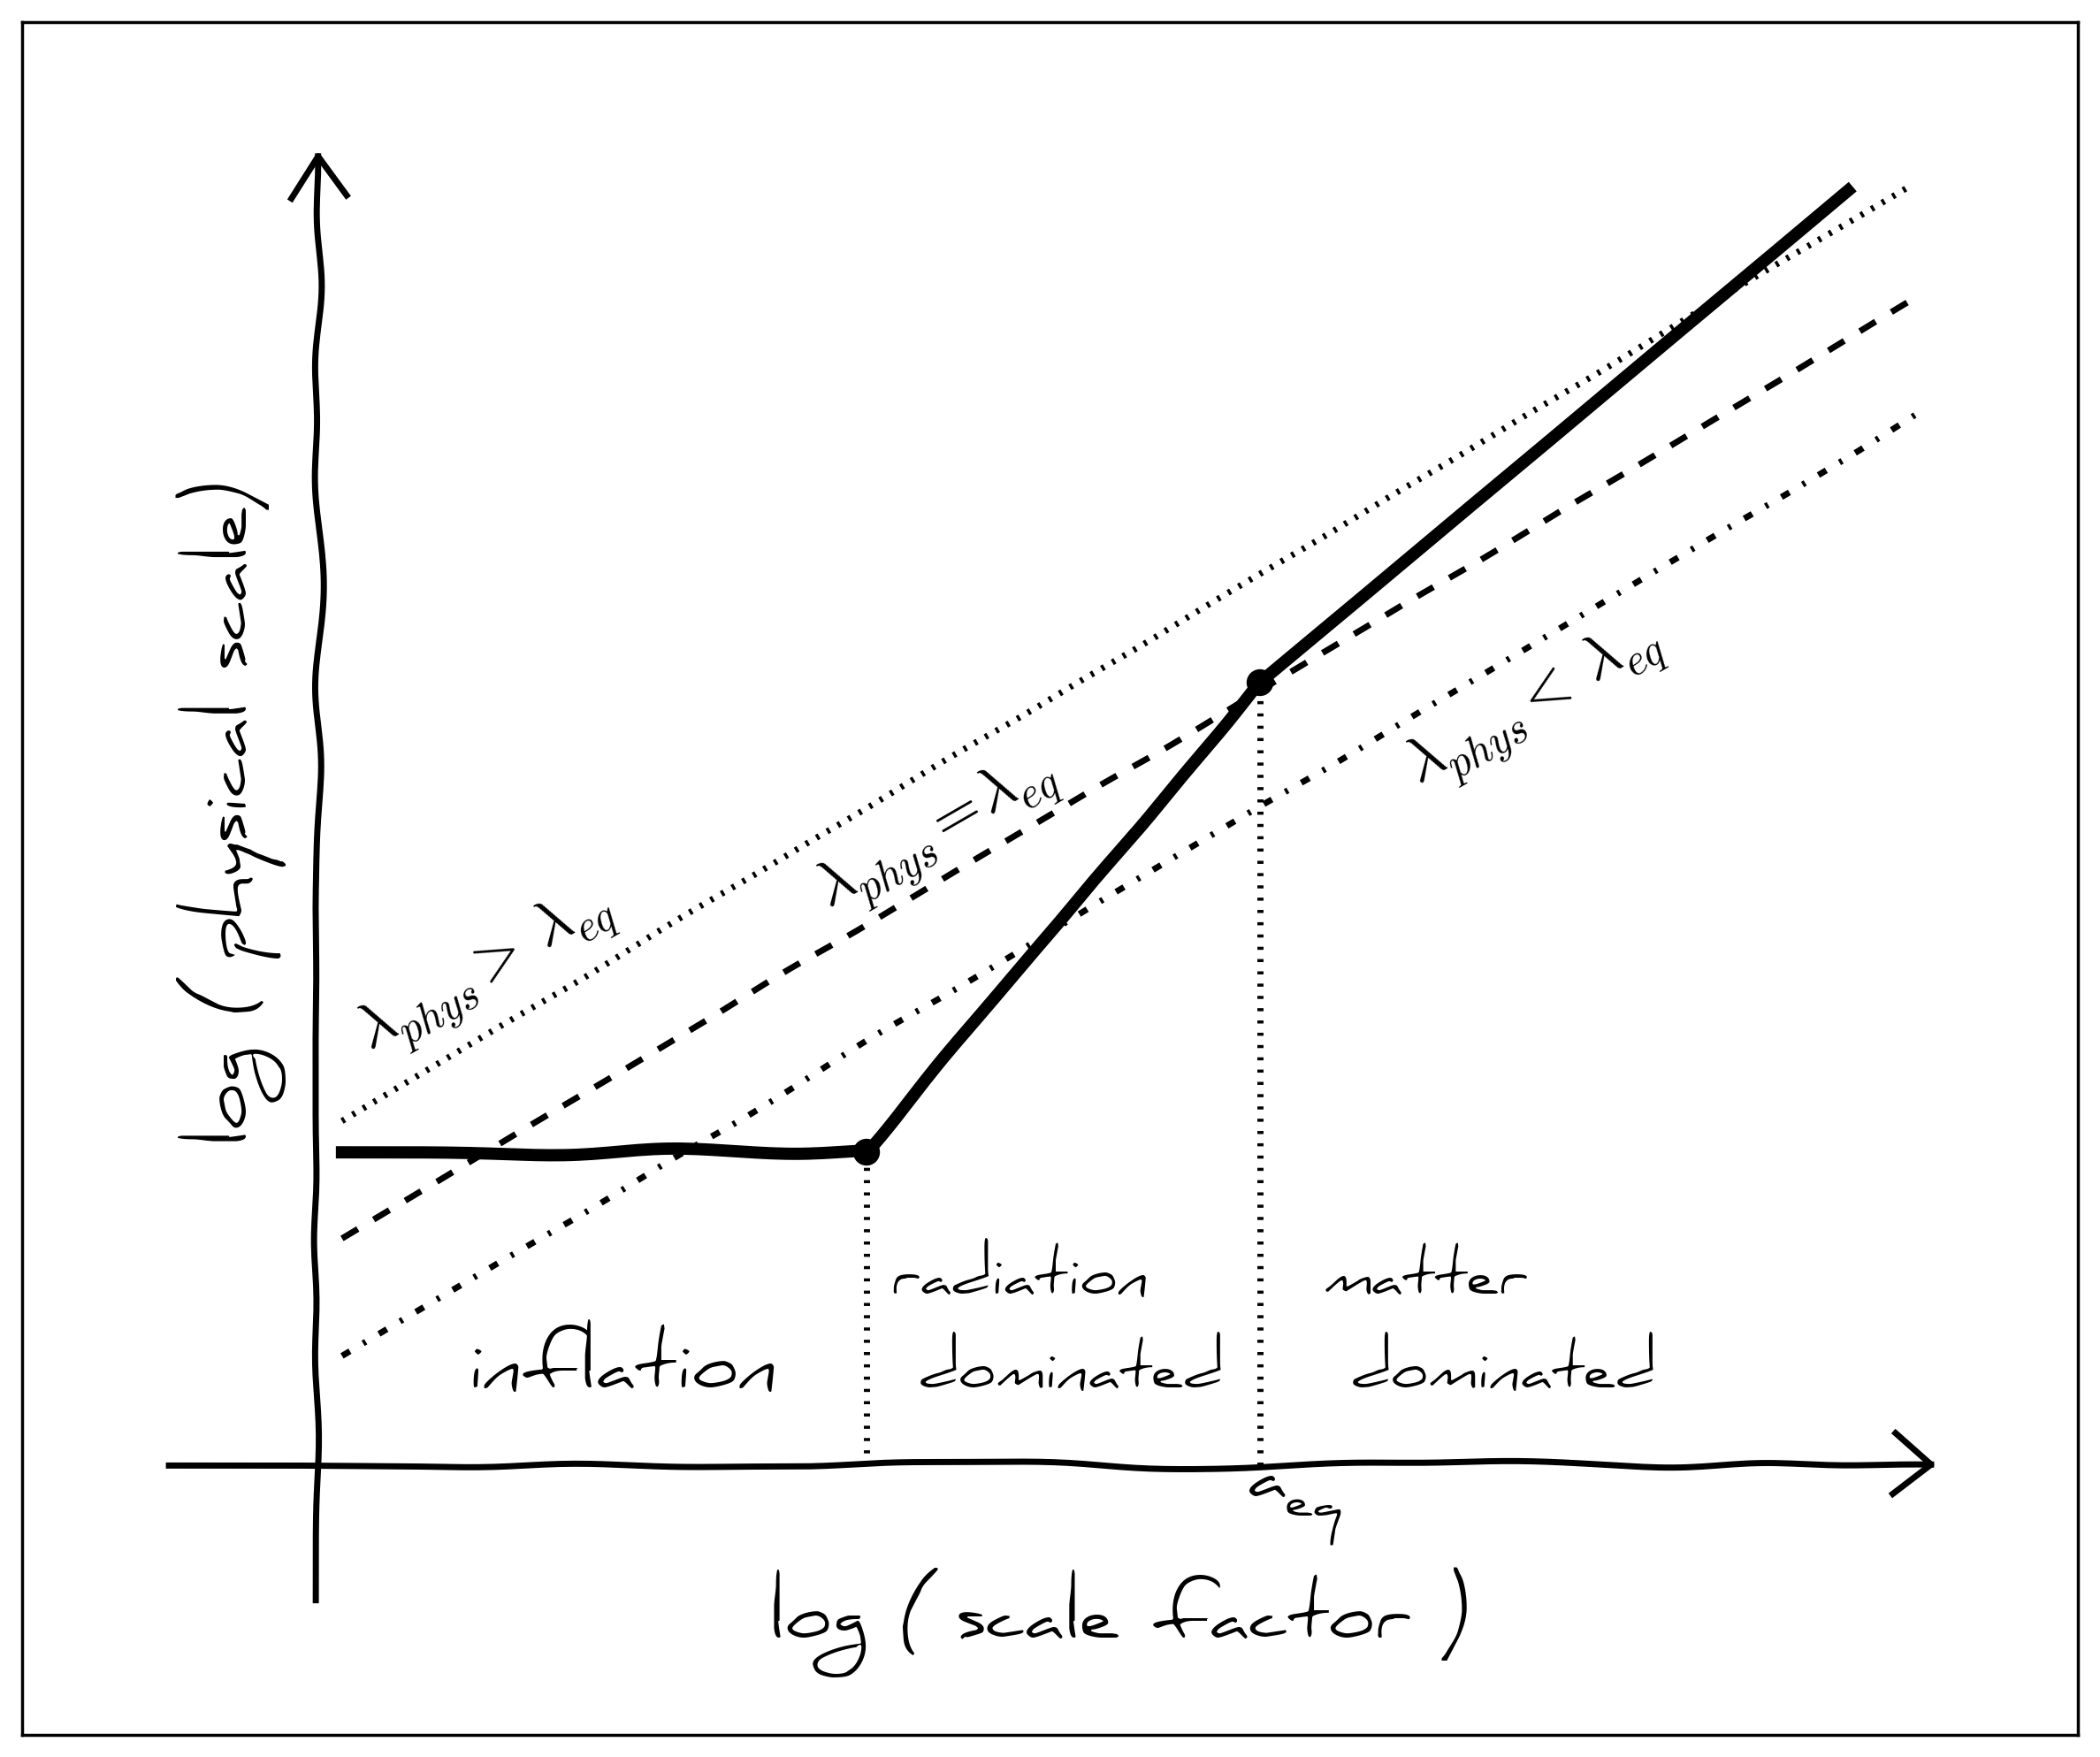
\includegraphics[width=\textwidth]{figs/lifo.png}
\caption{Schematic diagram that illustrates the evolution of the Hubble radius
(Above) The evolution of the Hubble radius (solid line) during inflation (flat), radiation
domination, and matter domination (note inflection). Dashed, dotted, and dot-dashed
lines show the physical length of three constant comoving scales. The scale corresponding
to the current Hubble radius cH−1
0 first “left the horizon” about 60 e-folds before the end
of inflation (open circle).
} \label{fig:lifo}
\end{center}
\end{figure*}

\todo{paragraph about how because D and T depend on cosmological parameters 
    so powerspectrum measurements of the matter density fluctuation can be 
    used a tests of the cosmological models.
}
So powerspectrum measurements of the matter density fluctuations can be compared
to predictions of various cosmological models in order to produce constraints 
on cosmological parameters, better understand dark energy, and test theories of 
gravity. Unfortunately, most of the matter in the Universe is in the form of dark 
matter and does not interact with radiation. 

Observers cannot measure the spatial statistics (or clustering) of dark matter 
directly. Instead, we measure the clustering of galaxies and quasars, which trace
the underlying matter distribution. The smoothed galaxy/quasar density field is 
approximated by a local function of the matter density field
\beq
\delta_g({\bf r}) = F( \delta({\bf r} ). 
\eeq
This function can then be expanded Taylor series,
\beq
\delta_g({\bf r}) = \sum\limits_{k=0}^{\infty} \frac{b_k}{k!} \delta^k. 
\eeq
$b_1$ is referred to as the linear bias factor and $b_0$ is chosen so that
$<\delta_g> = 0$. To linear order, 
\beq
P_g(k) = b_1^2 P(k). 
\eeq
The primary subpopulation of galaxies used so far for LSS studies are luminous 
red galaxies (\todo{Eistenstien apper}). These galaxies have $b_1 > 1$, which 
means they are {\em biased} tracers of the matter distribution (\todo{cite Zehavi 2005, Sheldon 2009, Gastanage 2009}). 
This bias is caused by the fact that luminous galaxies reside in larger potential 
wells, which have stronger clustering properties than than less massive ones (\todo{manera 2010}). 

Based on the simplified derivation of this section, once we have the spatial 
distribution of galaxies or quasars we can derive the clustering of the matter
distribution and then infer cosmological constraints. In practice, however, a
number of factors complicate this procedure. One key complication is redshift-space
distortions, which will be discussed in the following section.

\section{Redshift-Space Distortions} \label{sec:rsd}
Spectroscopic redshifts surveys, such as 2dFGRS, SDSS, and BOSS, have mapped out
millions of distant galaxies. Current surveys such as Extended Baryon Oscillation 
Spectroscopic Survey (eBOSS; \citealt{Dawson:2015aa}), and future surveys such as 
the Dark Energy Survey Instrument (DESI; \citealt{Schlegel:2011aa, Morales:2012aa, Makarem:2014aa}) 
and the Subaru Prime Focus Spectrograph (PFS; \citealt{Takada:2014aa}), will 
continue to map out millions more. These surveys dominate LSS studies and have/will 
been critical for inferring precise cosmological constraints. As their name suggest, 
however, these {\em redshift} surveys do not directly measure the position of 
galaxies, but rather the angular positions (right ascension and declination) and
redshift of galaxies. 

Redshifts from spectroscopic surveys observe the combination of recession 
velocities due to the expansion of the Universe and the peculiar velocities of the galaxies 
\beq
z_{obv} = z_{true} +  \frac{v_{pec}}{c}.
\eeq 
The comoving positions derived from the angular positions and redshifts are then
in {\em redshift-space} and ``distorted'' compared to real-space comoving positions:
\beq
{\bf s} = {\bf x} +  \frac{{\bf v}_{pec} \cdot \hat{n}}{H_0}.
\eeq 
$\hat{n}$ is the unit vector along the line-of-sight. Thankfully, all hope is not 
lost. The peculiar velocities of galaxies should be directly related to the total 
matter distribution, since galaxies can be thought of as test particles in a 
gravitational field. 

\todo{Kaiser 87} derives an approximation for the distortion caused by the coherent 
infall of galaxies onto over dense regions in redshift space. This redshift-space 
distortion (RSD), often referred to as the Kaiser effect, causes overdense regions
to appear squashed along the line of sight in redshift space. Galaxies around an
overdense region closest to the observer (us) are moving towards the center of the 
overdense region, so they appear in redshift-space to be farther away. Galaxies 
on the other side of the overdense region are moving towards it and the observer, 
so they appear closer to us. 

More precisely, the relation between the overdensity field in redshift-space can be 
derived from the continuity equation and the distant observer approximation, 
\beq
\delta^{(s)}({\bf k}) = (1 + f \mu^2) \delta({\bf k}).
\eeq
$f$ here is the growth rate of structure from Eq.~\ref{eq:f_growth} and 
$\mu = {\bf k} \cdot \hat{n} / k$, cosine of the angle between $k$ and 
the line of sight. 

The Kaiser effect can be combined with the galaxy bias model from 
Section~\ref{sec:lss}, in order to express the galaxy overdensity field in 
redshift-space:
\beq
\delta_g^{(s)}({\bf k}) = (b + f \mu^2) \delta({\bf k}).
\eeq
The redshift-space powerspectrum of the galaxy overdensity field can then be
written as 
\beq
P_g^{(s)}(k, \mu) = (b + f \mu^2)^2 P(k).
\eeq
On large scales and with small overdensities, the effect of redshift-space 
distoritons is well described by the Kaiser effect. On small scales with large
overdensities things get a little more complicated. 

The random peculiar velocities of galaxies in gravitationally bound structures 
such as clusters cause their position in redshift-space along the line-of-sight 
to be smeared out to larger scales.  This effect can easily be identified by 
eye in galaxy redshift maps. The elongations of the galaxy positions along the 
line-of-sight look like fingers pointing towards the observer. Hence this 
redshift-space distorion is called the ``fingers-of-god''. Its impact on the 
powerspectrum, is typically quantified using an overall exponential factor such as 
\beq
P_g^{(s)}(k, \mu) \approx e^{-f^2 \sigma_v^2 \mu^2 k^2} (b + f \mu^2)^2 P(k).
\eeq
$\sigma_v$ is a paramter quantifying the strength of the effect and is usually
left as a free parameter. 

The relations that quantify the impact of RSDs reveal another means of measuring 
$f$. Consider the Legendre expansion of $P_g^{(s)}(k, \mu)$, 
\beq
P_g^{(s)}(k, \mu) = \sum\limits_{\ell=0, 2, 4 ...} \mathcal{L}_\ell(\mu) P_g^\ell(k). 
\eeq
Each of the powerspectrum ``multipoles'' of this expansion can be written as 
\beq
P_g^{\ell}(k) = \frac{2 \ell + 1}{2} \int\limits_{-1}^{1} {\rm d}\mu \; P_g^{(s)}(k, \mu) \mathcal{L}_\ell(\mu).
\eeq
The powerspectrum multipoles for $\ell= 0$ (monopole) and $2$ (quadrupole), neglecting 
the figers-of-god which does not significantly impact larger scales, are
\beqa
P_g^0 (k) = (b_1^2 + \frac{2}{3} f b_1 + \frac{1}{5}f^2) P(k) \\
P_g^2 (k) = (\frac{4}{3} f b_1 + \frac{4}{7} f^2) P(k). 
\eeqa
Their ratio 
\beq \label{eq:multipole_ratio}
\frac{P_g^2}{P_g^0} = \frac{\frac{4}{3} f b_1 + \frac{4}{7} f^2}{b_1^2 + \frac{2}{3} f b_1 + \frac{1}{5}f^2},
\eeq
illustrates how the distortions caused by RSDs allow us to extract information of 
$f$ through measurements of the redshift-space galaxy powerspectrum!  

\section{Weighting Neutrinos with Galaxies} \label{sec:mneut}
Beyond providing a way to infer the growth rate of structure, which 
can be used to test GR and modified gravity scenarios, galaxy clustering
also provides a unique window to probe fundamental physics beyond the 
standard model. 
In the derivations of Sections~\ref{sec:lss} and~\ref{sec:rsd} we focused 
on how the density fluctuations of dark matter evolves. Because dark matter 
consistutes majority of the matter in the Universe, this is an excellent 
approximation. However, it negelects some of the more detailed imprints on 
large-scale structure from other matter components-- \emph{i.e.} neutrinos. 
Oscillation and detection experiments have (\emph{very} Nobel Prize in Physics 2015) 
convincingly confirmed {\em not} massless (\todo{Beringer et al. 2012,Lesgourges, 2012, 2013})

In the very early Universe, neutrinos are relativistic and coupled to the 
primordial plamsa. Later they decouple from the plasma, while they are still 
ultra-relativistic and redshift. While they are relativistic, they do not 
contribute to the energy density of matter but instead radiation. Then during 
matter domination, neutrinos eventually become non-relativistic. At this point, 
neutrinos contribute to the matter energy density and act as ``warm/hot'' 
dark matter.

Neutrinos after they decouple from the primoridal plasma constitutes a 
collisionless fluid, where the individual particles free-stream with 
characteristic velocities defined by their thermal velocity. While 
neutrinos are relativistic, their free-streaming scale is simply 
equal to the Hubble radius. But when they become non-relativistic, 
their can be expressed as
\beq
v_{\rm th} \approx 158 (1 + z) \left(\frac{1 {\rm eV}}{m} \right) \; \; {\rm km \; s^{-1}}
\eeq
and the free-streaming scale can be derived in an analogous way as
Jean's length
\beq
\lambda_{\rm FS} = 2 \pi \sqrt{\frac{2}{3}} \left( \frac{v_{\rm th}}{H} \right)
\eeq
or 
\beq \label{eq:kfs}
k_{\rm FS} = \frac{2\pi a}{\lambda_{\rm FS}} \approx  0.82 \frac{\sqrt{\Omega_\Lambda + \Omega_m(1+z)^3}}{(1+z)^2} \left(\frac{m_\nu}{1\;{\rm eV}} \right).
\eeq
$\Omega_\Lambda$ and $\Omega_m$ are the current cosmological constant and matter 
density fractions, respectively.

Neutrinos leave two main imprints on LSS. In the early Universe they contribute
to the radiation energy density. After they become non-relativistic in matter
domiation, they contribute to the matter energy density. As described in 
Section~\ref{sec:lss}, matter-radiation equality marks the turning point in 
suppression of growth of structure, quantified by $T(k)$. The transition of 
neutrinos from radiation to matter impacts $a_{eq}$ and thus shifts the turning 
point of the cold dark matter (CDM) only powerspectrum. 
Even after becoming non-relativistic, neutrinos do not contribute to the
clustering of matter on scale smaller than the free-streaming scale, 
$k_{\rm FS}$ (Eq.~\ref{eq:kfs}). The impact of this scale dependent 
suppression of clustering, can be analytically estimated for the powerspectrum: 
\beq
\frac{\Delta P}{P} = \frac{P^{f_\nu \neq 0} - P^{f_\nu = 0}}{P^{f_\nu = 0}} \approx - 8 f_\nu \;\;\;\; {\rm for}\;\; k \gg k_{\rm FS}.
\eeq
$f_\nu = \Omega_\nu / \Omega_m$.

The total mass of neutrinos (\mneut) dictate the strength of these imprints. 
The broadband shape of the powerspectrum offers a unique opportunity to measure
the extent of these imprints and constrain \mneut. The same tools that we 
use for analyzing RSDs and measuring the growth rate of structure can be used 
to measure \mneut from observations of galaxy surveys.
Based on their forecasts (DESI; \todo{cite}), the next galaxy surveys have the
potential to infer the most stringent constraints 
($\sigma_{\sum m_\nu} \sim 0.03\;{\rm eV}$) on \mneut. Such constraints would 
trump those from particle physics experiments (\todo{Wolf}) and have the potential to distinguish
between the normal or invereted neutrino mass hierarchy and reveal physics
beyond the Standard Model.

\section{Analyzing Galaxy Clustering}
%Beyond the general description and derivation of the redshift-space galaxy powerspectrum, the rest of galaxy clustering analysis in LSS studies follows the standard approach to Bayesian parameter inference. 
The ultimate goal of galaxy clustering analyses is to derive constraints on cosmological 
parameters and models from observed measurements of galaxly clustering -- the probability 
distribution of the cosmological parameters (\emph{e.g.} $f$, \mneut) given observations. 
The standard approach to deriving this {\em posterior} probability distribution is using 
Bayesian parameter inference. Based on Bayes theorem, the posterior probability distribution 
can be expressed as 
\beq
P({\bf \theta}| {\bf D}) = \frac{P({\bf D}|{\bf \theta}) P({\bf \theta})}{P({\bf D})}.
\eeq
${\bf D}$ and ${\bf \theta}$ refer to observations and cosmological parameters, respectively. 
$P({\bf D}|{\bf \theta})$, the probability distribution function for the observation ${\bf D}$ 
given model parameters ${\bf \theta}$ -- {\em i.e. likelihood function}, $\mathcal{L}$. 
$P({\bf \theta})$ is the {\em prior} probability distribution function. Lastly, $P({\bf D})$ 
is the ``evidence'', which for our purposes, is just a normalization factor independent of
${\bf theta}$. More commonly the equation above is more simply written 
\beqa \label{eq:bayes} 
P({\bf \theta}| {\bf D}) &\propto& P({\bf D}|{\bf \theta}) P({\bf \theta}) \\
{\rm posterior} &\propto& {\rm likelihood}\; \times \; {prior}.
\eeqa

In the context of galaxy clustering analyses and LSS cosmology in general, the likelihood 
function is {\em typically} assumed to have Gaussian function form and calculated as 
\beq \label{eq:likelihood}
P({\bf D}|{\bf \theta}) = \mathcal{L} = \frac{1}{(2\pi)^{N_d/2}\; {\rm det}{\bf C}^{1/2}}\; {\rm exp}\left[ -\frac{1}{2} ({\bf D} - F({\bf \theta}))^T {\bf C}^{-1} ({\bf D} - F({\bf \theta}))\right].
\eeq
${\bf D}$ is data from observations with dimension $N_d$. $F({\bf \theta})$ is the model prediction 
of the observable generated from cosmological parameters ${\bf \theta}$. And ${\bf C}$ is 
the covariance matrix. ${\bf D}$ is observed and measured from galaxy surveys. $F({\bf \theta})$
is broadly described by the derivations earlier this section. The covariance matrix ${\bf C}$
can be estimated using a number of different methods. 

Efforts to analytically estimate the covariance matrix from theory have been made in the past
(Hamilton, Rimes Scoccimarro 2006; Sefusatti et al. 2006; Pope Szapudi 2008; de Putter et al. 2012). 
Non-linear evolution, shot-noise, RSDs, and mapping between galaxies and matter, however,
complicate accurate estimations. Jack-knife resampling is another method for estimating 
covariances -- directly from data (Krewski 1981; Shao and Tu 1995). However, the method 
requires a number of arbitrary choices and cannot account for fluctuations on the scale 
of the survey (Norberg 2009). Instead, the latest analysis have estimated the ${\bf C}$ 
from a large number of galaxy mock catalogs generated from $N$-body simulations. For 
accurate estimation, typically, an order of $\sim 1000$ mock galaxy catalogs are used (\todo{Anderson, Beutler, DR13 papers}).
In fact, developing fast and accurate galaxy mock catalogs is a subfield of its own 
(\todo{cite a bunch of mock catalog papers}). 

From ${\bf D}$, $F(\boldsymbol{\theta})$, and ${\bf C}$ we have the likelihood of 
Eq.~\ref{eq:likelihood}. As an added detail, the ${\bf C}$ estimate from above is 
biased depending on factors such as $N_d$ \citep{hartlap2007}. Standard analyses 
include a correction -- the Hartlap factor -- to the covariance matrix estimate. Once the 
likelihood is evaluated, since the prior probability distribution is chosen, the posterior 
probability distribution functions of the cosmological parameters is essentially already 
evaluated. In practice, instead of evaluating the posterior distribution at all points in 
parameter space, the distribution is sampled using a sampler such as a Markov Chain Monte 
Carlo (MCMC) sampler -- \emph{e.g.} $\mathtt{emcee}$ \citep[][]{emcee}.

From the galaxy clustering analysis I generally describe in this chapter, the latest 
galaxy surveys have produced remarkable constraints on cosmological parameters. 
From observations of SDSS and BOSS, measurements of the powerspectrum multipoles 
($\ell = 0, 2,\;{\rm and}\;4$) have yielded a number of constraints on $f\sigma_8$ 
(\todo{cite Oka 2014, Beutler 2017}). Analogous configure-space analyses
have derived similar $f \sigma_8$ constraints (\todo{Reid, Alam:2016}). $\sigma_8$ 
is the amplitude of the powerspectrum on the scale of $8\;h^{-1}{\rm Mpc}$. 
Similar to multipoles, powerspectrum wedges have also been used to derive $f\sigma_8$ 
constraints in both Fourier and configuration-space (\todo{Sanchez2017, Grieb2017}). 
\todo{also cite Samushia2015, Beutler2014, Chuang2014, Sanchez2013, Reid2014, More2015}

The $f \sigma_8$ constraints can then be used to test $\Lambda$CDM cosmology and 
General Relativity through comparisons with cosmological model predictsions from 
Cosmic Microwave Background (CMB) experiments such as WMAP (\todo{cite WMAP look at florian}) or {\em Planck} (\todo{cite planck collaboration}).
The constraints from BOSS are generally consistent $\Lambda$CDM and GR over 
$0.2 < z < 0.75$ (\todo{cite stuff}).  For reference, \todo{cite Beutler} derives 
$f\sigma_8 = 0.482 \pm 0.053, 0.455 \pm 0.050$, and $0.410 \pm 0.042$ for effective redshift 
$z_{\rm eff} = 0.38, 0.51$, and $0.61$ from BOSS. $f \sigma_8$ constraints from 
galaxy powerpsectrum multipole analyses have also been combined with CMB data to 
constrain \mneut (\todo{Beuter:2014 and Gil-Marin:2015}).

%Cosmological measurements such as galaxy clustering statistics are no longer dominated by uncertainties from statistical precision, but from systematic effects of the measurements. This is a result of the millions of redshifts to distant galaxies that have been obtained through redshift surveys such as the 2dF Galaxy Redshift Survey (2dFGRS; \citealt{Colless:1999aa}) and the Sloan Digital Sky Survey III Baryon Oscillation Spectroscopic Survey 
Ongoing and future surveys, such as the Extended Baryon Oscillation Spectroscopic 
Survey (eBOSS; \todo{Dawson:2015aa}), the Dark Energy Survey Instrument 
(DESI; \todo{Schlegel:2011aa, Morales:2012aa, Makarem:2014aa}), 
and the Subaru Prime Focus Spectrograph (PFS; \todo{Takada:2014aa}), will 
continue to collect many more million redshifts and expand the probed cosmic 
volume by an order of magnitude. These observations have the potential to 
produce cosmologicl parameter constraints with unprecedented statistical 
precision. The main challenges now for realizing the full potential of 
these observations are methodological.

%\todo{briefly mention future surveys and how we're no longer statistics dominated but rather  systematic dominated. just the usual postdoc application stuff for motivating my phd.  higher order statistics, systematics, innovative methods for inference}

So far I have mainly focused on LSS analyses using only the two-point
statistic -- \emph{i.e.} the galaxy powerspectrum. Analyses restricted
to just the two-point statistic, however, face a number of limitations. 
The constraints on the growth rate of structure, I quote above, have all 
been constraints on $f \sigma_8$ rather than $f$ alone. The degeneracy 
between $f$ and $\sigma_8$, the amplitude of $P(k)$, cannot be broken 
with $P(k)$ alone. Furthermore, the $P(k)$ multipoles in 
Eq.~\ref{eq:multipole_ratio} demonstrate that $P(k)$ analyses also 
suffer from the degeneracy between $f$ and bias parameters. 

The {\em bispectrum} $B({\bf k})$, three-point statistic of density
fluctuations, can be used to break the degeneracies between $f$, 
$\sigma_8$, and bias parameters.
\todo{Scoccimarro et al. 1998a; Verde et al. 1998; Scoccimarro 2000 see Bernardeau2002 for a review}.
The dependence on triangle configuration in $B(⃗{\bf k})$ 
disentangles contributions from gravitational instability versus 
non-linear biasing of galaxies. Without going into any further detail, 
in Figure\todo{figure} I present the $B({\bf k})$ measurement for 
the BOSS Data Release 12 CMASS (this is not an acronym) galaxy sample 
(left) and a perturbation theory model (right). $P(k)$ and $B({\bf k})$ 
can be jointly analyzed in order to derive constraints explicitly on $f$. 

Before proceeding with any of the above analyses, observational systematic 
effects must be robustly accounted for. Fiber-fed multi-object spectroscopic 
surveys (\emph{e.g.} SDSS, BOSS, eBOSS, DESI, and PFS), typically suffer
from incompleteness from stellar density, incompleteness from seeing, 
fiber collisions, and redshift failures (\todo{Ross:2012, Anderson:2012}) 
If unaccounted, fiber collisions, for instance, prevent surveys from 
collecting a significant fraction redshifts due to physical constraints 
on the focal plane. Their impact on $P(k)$ is well beyond their angular scale 
and restricts analysis on small scales, which has higher signal-to-noise. 
In addition to discarding the statistical gains of these surveys, fiber 
collisions can also bias the constraints on cosmological parameters. 
Fortunately, challenges from observational systematics are often {\em solvable}
\citep[][and \chap{fc}]{Ross:2012aa, Guo:2012aa}.

The likelihood of Eq.~\ref{eq:likelihood}, assumes a Gaussian functional form
-- a standard assumption in LSS analyses. This assumption for LSS with galaxies, 
in detail, cannot be correct due to nonlinear gravitational evolution and 
biasing~\citep{Bernardeau:2002aa}. Furthermore, to capture the sample variance of the data
the likelihood relies on the covariance matrix estimate, which currently 
faces a number of shortcomings. Besides the labor and computational costs 
of the required simulated mock catalogs, mock catalogs are inaccurate on small scales~(see 
\citealt{cosmiccode,nifty} and references therein). Furthermore, using covariance 
matrix estimates rather than the ``true'' covariance matrix \citep{Sellentin:2016a}
along with systematics impact the likelihood in ways difficult to model. 
Evaluating the explicit likelihood, however, is not necessary for inferring
cosmological parameters. Likelihood-free inferences such as Approximate 
Bayesian Computation (ABC) relax these restrictions and make inference 
possible without making any assumptions on the likelihood (\chap{abc}).

As described earlier in this Chapter, galaxies are biased tracers of the 
underlying matter distribution. For more than a decade, halo occupation 
modeling has been the main framework for connecting galaxies
to the dark matter structures underneath in galaxy formation and cosmology
studies (\todo{Yang et al. 2003; Tinker et al. 2005; Zehavi et al. 2005; Porciani  Norberg
2006; van den Bosch et al. 2007; Zheng et al. 2007; Conroy
 Wechsler 2009; Yang et al. 2009; Zehavi et al. 2011;
Guo et al. 2011; Wake et al. 2011; Yang et al. 2011, 2012;
Leauthaud et al. 2012; Rodr´ıguez-Puebla et al. 2012; Tinker
et al. 2013; Cacciato et al. 2013; More et al. 2013;
Guo et al. 2014; Zu Mandelbaum 2015}). The standard halo occupation model
assumes that galaxies reside in dark mater halos and their occupation 
is function of the mass of the halo. However, the clustering of dark 
matter halos, which themselves are tracers of the density field, 
depend on properties beyond their masses. If this effect, coined 
{\em halo assembly bias}, propagates to galaxies, it will induce 
{\em galaxy} assembly bias on standard halo occupaiton model and 
significantly impact galaxy clustering analyses (\todo{Zentner:2014}). 

Beyond their utility as tracers for cosmological analyses, galaxies 
also pose fundamental questions regarding how the early homogenous 
Universe became the heterogenous one today. Observations have now 
firmly established a global view of galaxy properties out to $z\sim1$ 
\citep[\emph{e.g.}][\chap{galenv}]{Blanton:2009aa, Moustakas:2013aa}.
These observations can be positioned in the hierarchical structure 
formation framework in order to constrain key elements of galaxy evolution 
\citep[][\chap{galhalo}]{Wetzel:2013aa}. 

\todo{galaxy-halo connection: 
start by talking about the galaxy-halo model now. Talk about the evidence 
that this simpe model is failing. Then talk about how deviations from this 
model (e.g. assembly bias) impacts the accuracy of mock catalogs and also 
the cosmological constraints we derive. Then talk about how this is important 
for galaxy evolution, which is interesting on its own. Talk about the role 
of galaxy enviornment in their evolution. }

\todo{some summarizing remarks}

\chapname s~\chapalt{fc} and~\chapalt{galenv} have both been refereed and
published in the astronomical literature.
\chapname s~\chapalt{abc} and~\chapalt{galhalo} have been refereed and accepted 
to the \emph{Monthly Notices of the Royal Astronomical Society} and \emph{The Astrophysical Journal},
respectively. All of these \chapname s were co-authored with collaborators but the majority
of the work and writing in each \chapname\ is mine. Below, I describe my contributions to each \chapname:
\begin{enumerate}

{\item 
For \chap{fc}, I developed the idea for the project in collaboration with Roman
Scoccimarro and Michael Blanton. I implemented the project with contributions 
from Roman Scoccimarro. The project utilized simulation data from Jeremy Tinker
and Sergio Rodr\'{i}guez-Torres. I wrote the paper with additions from 
Roman Scoccimarro and edits by Michael Blanton. 
}

{\item 
For \chap{abc}, I developed the idea for the project in collaboration with 
Mohammadjavad Vakili, Andrew Hearin, and David Hogg. I implemented the project 
with Mohammadjavad Vakili and contributions from Andrew Hearin and Kilian Walsh.
The project utilized software written by Andrew Hearin and Duncan Campell. 
I wrote the paper together with Mohammadjavad Vakili with additions from
Andrew Hearin, David Hogg, and Kilian Walsh.
}

{\item 
For \chap{galenv}, I developed the idea for the project in collaboration with 
Michael Blanton. I implemented the project using catalogs constructed by 
John Moustakas from observations made by the PRIMUS collaboration (Alison Coil,
Richard Cool, Daniel Eisenstein, Ramin Skibb, Kenneth Wong, and Guangtun Zhu).
I wrote the paper with additions from Michael Blanton. 
}

{\item 
For \chap{galhalo}, I developed the idea for the project in collaboration with 
Jeremy Tinker. I implemented the project using simulation data from Andrew 
Wetzel. I wrote the paper with comments and edits by Jeremy Tinker and Andrew 
Wetzel. 
}
\end{enumerate}


\chapter{Theory \chaplabel{theory}}

\section{Galaxy Clustering} 

\section{The Galaxy Bispectrum} 

\renewcommand{\chapid}{obvs}

\chapter{The Effect of Fiber Collisions on the Galaxy Power Spectrum Multipoles}

This \paper\ is joint work with Roman~Scoccimarro (NYU), 
Michael~R.~Blanton (NYU), Jeremy~L.~Tinker (NYU), and Sergio Rodr\'{i}guez-Torres 
(Universidad Aut\'{o}noma de Madrid) published in \emph{Monthly Notices of the Royal
Astronomical Society}. 

\newcommand{\beqa}{\begin{eqnarray}}
\newcommand{\eeqa}{\end{eqnarray}}

\newcommand{\lexp}{\mathop{\langle}}
\newcommand{\rexp}{\mathop{\rangle}}
\newcommand{\rexpc}{\mathop{\rangle_c}}
\def\k{{\hbox{\BF k}}}
\def\x{{\hbox{\BF x}}}
\def\r{{\hbox{\BF r}}}
\def\s{{\hbox{\BF s}}}
\def\la{\mathrel{\mathpalette\fun <}}
\def\ga{\mathrel{\mathpalette\fun >}}
\def\fun#1#2{\lower3.6pt\vbox{\baselineskip0pt\lineskip.9pt
\ialign{$\mathsurround=0pt#1\hfill##\hfil$\crcr#2\crcr\sim\crcr}}}

\newcommand{\beq}{\begin{equation}}
\newcommand{\eeq}{\end{equation}}

%\title{The Effect of Fiber Collisions on the Galaxy Power Spectrum Multipoles} 

\section{Chapter Abstract}
\qquad Fiber-fed multi-object spectroscopic surveys, with their ability to collect an unprecedented number of redshifts, currently dominate large-scale structure studies. However, physical constraints limit these surveys from successfully collecting redshifts from galaxies too close to each other on the focal plane. This ultimately leads to significant systematic effects on galaxy clustering measurements. Using simulated mock catalogs, we demonstrate that fiber collisions have a significant impact on the power spectrum, $P(k)$, monopole and quadrupole that exceeds sample variance at scales smaller than $k\sim0.1~h/{\rm Mpc}$.

\qquad We present two methods to account for fiber collisions in the power spectrum. The first, statistically reconstructs the clustering of fiber collided galaxy pairs by modeling the distribution of the line-of-sight displacements between them. It also properly accounts for fiber collisions in the shot-noise correction term of the $P(k)$ estimator. Using this method, we recover the true $P(k)$ monopole of the mock catalogs with residuals of $<0.5\%$ at $k=0.3~h/{\rm Mpc}$ and $<4\%$ at $k=0.83~h/{\rm Mpc}$ -- a significant improvement over existing correction methods. The quadrupole, however, does not improve significantly.

\qquad The second method models the effect of fiber collisions on the power spectrum as a convolution with a configuration space top-hat function that depends on the physical scale of fiber collisions. It directly computes theoretical predictions of the fiber-collided $P(k)$ multipoles and reduces the influence of smaller scales to a set of nuisance parameters. Using this method, we reliably model the effect of fiber collisions on the monopole and quadrupole down to the scale limits of theoretical predictions. The methods we present in this paper will allow us to robustly analyze galaxy power spectrum multipole measurements to much smaller scales than previously possible.


\section{Introduction} 
Cosmological measurements such as galaxy clustering statistics are
no longer dominated by uncertainties from statistical precision, but from 
systematic effects of the measurements. This is a result of the millions of 
redshifts to distant galaxies that have been obtained through redshift surveys
such as the 2dF Galaxy Redshift Survey (2dFGRS; \citealt{Colless:1999aa}) and 
the Sloan Digital Sky Survey III Baryon Oscillation Spectroscopic Survey 
(SDSS-III BOSS; \citealt{Anderson:2012aa, Dawson:2013aa}). Current surveys, 
such as the Extended Baryon Oscillation Spectroscopic Survey (eBOSS; \citealt{Dawson:2015aa}), 
and future surveys such as the Dark Energy Survey Instrument (DESI; \citealt{Schlegel:2011aa, 
Morales:2012aa, Makarem:2014aa}), and the Subaru Prime Focus Spectrograph 
(PFS; \citealt{Takada:2014aa}), 
will continue to collect many more million redshifts, extending our measurements 
to unprecedented statistical precision. These completed and future surveys, all use 
and will use fiber-fed spectrographs. 
%All these surveys, both completed and future,  
%use fiber-fed spectrographs. 

%As of 2016, millions of redshifts to distant galaxies have been obtained 
%through redshift surveys. Cosmological measurements such as galaxy clustering 
%statistics are no longer dominated by uncertainties from statistical precision, 
%but from systematic effects of the measurements. These surveys, such as the 2dF 
%Galaxy Redshift Survey (2dFGRS; \citealt{Colless:1999aa}) and the Sloan Digital 
%Sky Survey III Baryon Oscillation Spectroscopic Survey (SDSS-III BOSS; 
%\citealt{Anderson:2012aa, Dawson:2013aa}), and future surveys, such as the 
%Extended Baryon Oscillation Spectroscopic Survey (eBOSS; \citealt{Dawson:2015aa}), 
%Dark Energy Survey Instrument (DESI; \citealt{Schlegel:2011aa, 
%Morales:2012aa, Makarem:2014aa}), and Subaru Prime Focus Spectrograph (PFS; \citealt{Takada:2014aa}), 
%use fiber-fed spectrographs. 

For each galaxy, a fiber is used to obtain a spectroscopic redshift. However, 
the physical size of the fiber housing and other physical constraints limit 
how well any of these surveys can observe close pairs of galaxies. In the SDSS, 
if two galaxies are located within the fiber collision angular scale from 
one another on the sky, separate fibers cannot be placed adjacently to 
observe them simultaneously 
(\citealt{Yoon:2008aa}). In these situations, only a single redshift 
is measured. With redshifts of galaxies in close angular proximity missing 
from the sample, any clustering statistic probing these scales will be 
systematically affected. 

As our cosmological surveys extend further to higher redshifts, the systematic
effect becomes more severe. The fiber collision angular scale corresponds 
to a larger comoving scale at higher redshift, thereby affecting our measurements on larger 
scales. BOSS, in particular, has an angular fiber collision scale 
of $62"$. This corresponds to $\sim 0.43 \;\mathrm{Mpc}/h$ at the 
center of the survey's redshift range; fiber-collided galaxies 
account for $\sim 5\%$ of the galaxy sample (\citealt{Anderson:2012aa, 
Reid:2012aa, Guo:2012aa}). 
While this may seem like a relatively small fraction of redshifts, its 
effect on clustering measurements such as the power spectrum and bispectrum 
is significant and needs to be accounted for in order to probe mildly non-linear scales. 
Unfortunately, future spectroscopic surveys such 
as DESI, which will use robotic fiber positioner 
technology, will be subject to similar effects. 
In fact, based on the DESI Final Design 
Report\footnote{DESI Final Design Report: \url{http://desi.lbl.gov/tdr/}}, which estimates that 
$\sim 6\%$ of Luminous Red Galaxies and 
$>20\%$ of Emission-Line Galaxies will be fiber-collided, 
fiber collisions will affect a {\em larger} fraction of the target 
sample than in BOSS.
Therefore, 
accounting for the effects of fiber collisions will remain a crucial and 
unavoidable challenge for analyzing clustering measurements. 

%Meanwhile, improvements in our modeling of clustering measurements continue 
%to extend the physical scales we can model. Galaxy power spectrum models
%continue to reliably model higher $k$ domains with improvements in the 
%non-linear regime. In 
%
%For instance, the $\mathtt{RegPT}$ model (\citealt{Taruya:2012aa}), which was used in a 
%recent analysis of power spectrum multipoles by \cite{Beutler:2014aa},
%can reliably probe up to $k = 0.28\;h/\mathrm{Mpc}$ at $z = 0.55$, the center 
%of the BOSS redshift range.  

To correct for fiber collisions, one common approach used in clustering 
measurements is the nearest neighbor method (\citealt{Zehavi:2002aa, Zehavi:2005aa, 
Zehavi:2011aa, Berlind:2006aa, Anderson:2012aa}). For fiber-collided galaxies without 
resolved redshifts, the method assigns the statistical weight of the 
fiber-collided galaxy to its nearest angular neighbor. This provides 
a reasonable correction for the fiber collision effects at scales much 
larger than the fiber collision scales; however the correction falls short 
elsewhere. In fact, as \cite{Zehavi:2005aa} find, 
fiber collisions affect the two-point correlation function (2PCF) 
measurements even on scales significantly larger than the fiber collision 
scale ( $> 1\;\mathrm{Mpc}/h$). 

For power spectrum measurements in BOSS, 
the nearest neighbor method has recently been supplemented with adjustments 
in the constant shot-noise term of the power spectrum estimator to correct 
for fiber collisions~\citep{Beutler:2014aa, Gil-Marin:2014aa, 
Gil-Marin:2016ab, Gil-Marin:2016aa, Beutler:2016aa, Grieb:2016aa}. More specifically, 
methods like the one used in 
\cite{Gil-Marin:2014aa} obtain the value of the shot-noise term from mock catalogs and thus rely entirely on their accuracy to correct for fiber collisions. 
This is concerning since, as we shall demonstrate in detail, fiber 
collisions depend systematically on the small-scale power spectrum, and mock catalogs used for large scale structure analyses are typically 
not based on high resolution N-body simulations. In addition, there is no way to validate and 
calibrate the shot-noise term independently for observations. A more 
reliable approach is to marginalize over the value of the shot-noise 
term, and this is the approach that has recently become more popular
~\citep{Gil-Marin:2016ab, Beutler:2016aa, Grieb:2016aa, Gil-Marin:2016aa}. 
However, adjustments to the shot-noise term are limited to the power spectrum monopole, since higher order multipoles do not have a shot-noise term. However, as we shall discuss in detail below, {\em fiber collisions affect all multipoles in a $k$-dependent way}, not just adding a constant for the monopole power.

\cite{Guo:2012aa}, focusing on SDSS-III BOSS like samples, proposed 
a fiber collision correction method for the 2PCF that is able to reasonably 
correct for fiber collisions above and below the collision scale. 
\cite{Guo:2012aa} estimates the total contribution of fiber-collided galaxies 
to the 2PCF by examining the pair statistics in overlapping tiling regions of 
the survey, where a smaller fraction of galaxies suffer from fiber collisions.
Unfortunately, applying an analogous method in Fourier space proves to be more difficult. 
The \cite{Guo:2012aa} method in Fourier space would involve measuring the power spectra 
for individual overlapping regions. Given the complex geometry of these 
regions, the systematic effect introduced by the window function makes 
measuring the power spectrum at larger scales intractable. 

%Applying an analogous method to Fourier space would first involve taking 
%power spectrum measurements of each overlapping and non-overlapping 
%region individually. Afterwards, the window function of those regions 
%would have to be deconvolved from the measurements in order to model 
%the power spectrum contribution from fiber collided galaxies. \todo{Unfortunately, 
%due to the complex geometry of the overlapping regions, the systematic effects of
%including the window function modeling the }

Meanwhile, galaxy redshift-space power spectrum models from perturbation theory continue to 
reliably model higher $k$ in the weakly non-linear regime
\citep{Taruya:2010aa, Taruya:2014aa, Okumura:2015aa, Beutler:2016aa, Grieb:2016aa, Sanchez:2016aa}.
%\citep{Taruya:2010aa, Sato:2011aa, Taruya:2012aa, Okumura:2012aa, Taruya:2013aa, Taruya:2014aa, Beutler:2014aa, Okumura:2015aa, Beutler:2016aa, Grieb:2016aa, Sanchez:2016aa}.
Recent analyses of galaxy power spectrum 
multipoles (\citealt{Beutler:2014aa, Gil-Marin:2014aa, Gil-Marin:2016ab, Gil-Marin:2016aa, Beutler:2016aa, Grieb:2016aa}) use scales up to $k_{\rm max}=0.15-0.2 h$/Mpc for BOSS galaxies, and this limit will for sure move towards smaller scales in upcoming analyses. As statistical errors decrease the importance of systematics due to fiber collisions plays an increasingly important role. The main goal of this paper is to quantify this systematic effect for the power spectrum multipoles and to provide ways to overcome it; for this purpose we
develop two distinct approaches. 

The first approach improves upon the nearest neighbor method by modeling the 
distribution of the line-of-sight displacement between resolved fiber collided 
galaxies to statistically reconstruct the clustering of fiber-collided galaxies. 
This uses information on resolved fiber collided galaxies that is available from 
the data themselves (e.g. in tiling overlap regions). The difficulty with this 
method is that it works statistically, i.e. we cannot reconstruct the {\em actual} 
galaxy by galaxy line of sight displacement due to collisions. As a result of this, 
while the method works very well to recover the true power spectrum monopole 
from fiber collided galaxy catalogs, it does not work sufficiently well for the 
power spectrum quadrupole which is far more sensitive to the precise structure of ``fingers of god''. 

The second approach addresses the shortcomings of the first one by modeling the effects of fiber collisions on the {\em predictions} instead of trying to undo their effect on the data before computing power spectrum statistics. It approximates the effect of fiber collisions on the 2PCF as 
a 2D top hat function. Then it derives the effect of fiber collisions on the galaxy power spectrum as a 
convolution of the true power spectrum with the top hat function. Therefore the theoretical predictions for the power spectrum are fiber collided and then can be compared  directly to the observed fiber collided power spectrum in clustering analyses. 

This paper is organized as follows. 
In Section \ref{sec:catalog}, we briefly describe the simulated mock catalogs 
with realistic fiber collisions and the power spectrum estimator used throughout 
the paper. We then demonstrate the impact of fiber collisions on power spectrum 
measurements and how the nearest neighbor method does not adequately account 
for fiber collisions in Section \ref{sec:fc_pk}. We present our two methods 
of accounting for fiber collisions along with the results for mock catalogs in 
Section \ref{sec:dlospeak} and Section \ref{sec:fourier}, respectively. Finally 
in Section \ref{sec:summary} we summarize our results and conclude. 

%%%%%%%%%%%%%%%%%%%%%%%%%%%%%%%%%%%%%%%%%%%%%%%%%%%%%%%%%%%%%%%%%%%%%%%%%%%%%%
% Fiber-collided Mock catalogs
%%%%%%%%%%%%%%%%%%%%%%%%%%%%%%%%%%%%%%%%%%%%%%%%%%%%%%%%%%%%%%%%%%%%%%%%%%%%%%
\section{Fiber-collided Mock catalogs} \label{sec:catalog}
For various purposes, such as characterizing the impact of the survey window function on statistics and estimating covariance matrices, simulated mock 
catalogs play a crucial role in interpreting  
clustering measurements of observed galaxies 
\citep[][also see citations in \citealt{Chuang:2015aa}]{ Cole:1998aa, Scoccimarro:2002aa, Anderson:2012aa, Beutler:2014aa, Carretero:2015aa}. 
%\citep{Cole:1998aa, Scoccimarro:2002aa, Yan:2004aa, Anderson:2012aa, Manera:2013aa,  Monaco:2013aa, Beutler:2014aa, Gil-Marin:2014aa, White:2014aa, Manera:2015aa, Tassev:2015aa, Carretero:2015aa, Howlett:2015aa, Izard:2016aa, Chuang:2015aa, Kitaura:2016aa, Munari:2016aa, Sunayama:2016aa}. 
They also provide a means of understanding systematic effects such as  
fiber collisions (\citealt{Guo:2012aa, Manera:2013aa}).
Since systematic effects can be simulated on them, they allow us to test 
how these effects influence clustering measurements and devise correction 
methods that attempt to account for these effects.

A direct way of understanding the effects of fiber collisions on clustering 
statistics in observations is to first apply fiber collisions to mock catalogs
and then compare the clustering statistics obtained from mock catalogs with 
and without the fiber collisions. Correction methods for fiber collisions can 
then be applied to the fiber-collided mocks. The merit of the correction 
method can be assessed by how successfully they reproduce the clustering statistics 
of the original mock catalogs without fiber collisions. The correction 
method can then be applied to the observed data with some assurance that it 
accounts for fiber collisions and improves the clustering measurements. 

When applying the fiber collisions to the mock catalogs, it is essential to 
apply them in the same manner they affect the observations. For BOSS, galaxies
within $62"$ are fiber-collided (\citealt{Anderson:2012aa}). In reality, 
this criteria is further complicated by the tiling scheme of observing 
plates that create overlapping regions, which have a higher success rate in 
resolving galaxy spectra within the fiber collision angular scale (\citealt{
Guo:2012aa, Reid:2012aa}). Furthermore, fiber collisions are only one of the 
systematic effects that influence BOSS data. Systematic effects include the 
unique geometry of the BOSS survey, the variable completeness in different areas  
covered by unique sets of spectroscopic plates, and redshift failures 
(\citealt{Anderson:2012aa, Ross:2012aa}). 

\def \cmasscolor{black}
\def \ldgcolor{blue}
\def \nseriescolor{orange}
\def \qpmcolor{blue}
\def \tmcolor{green}
\def \bmdcolor{red}

% FIGURE %%%%%%
\begin{figure}
\begin{center}
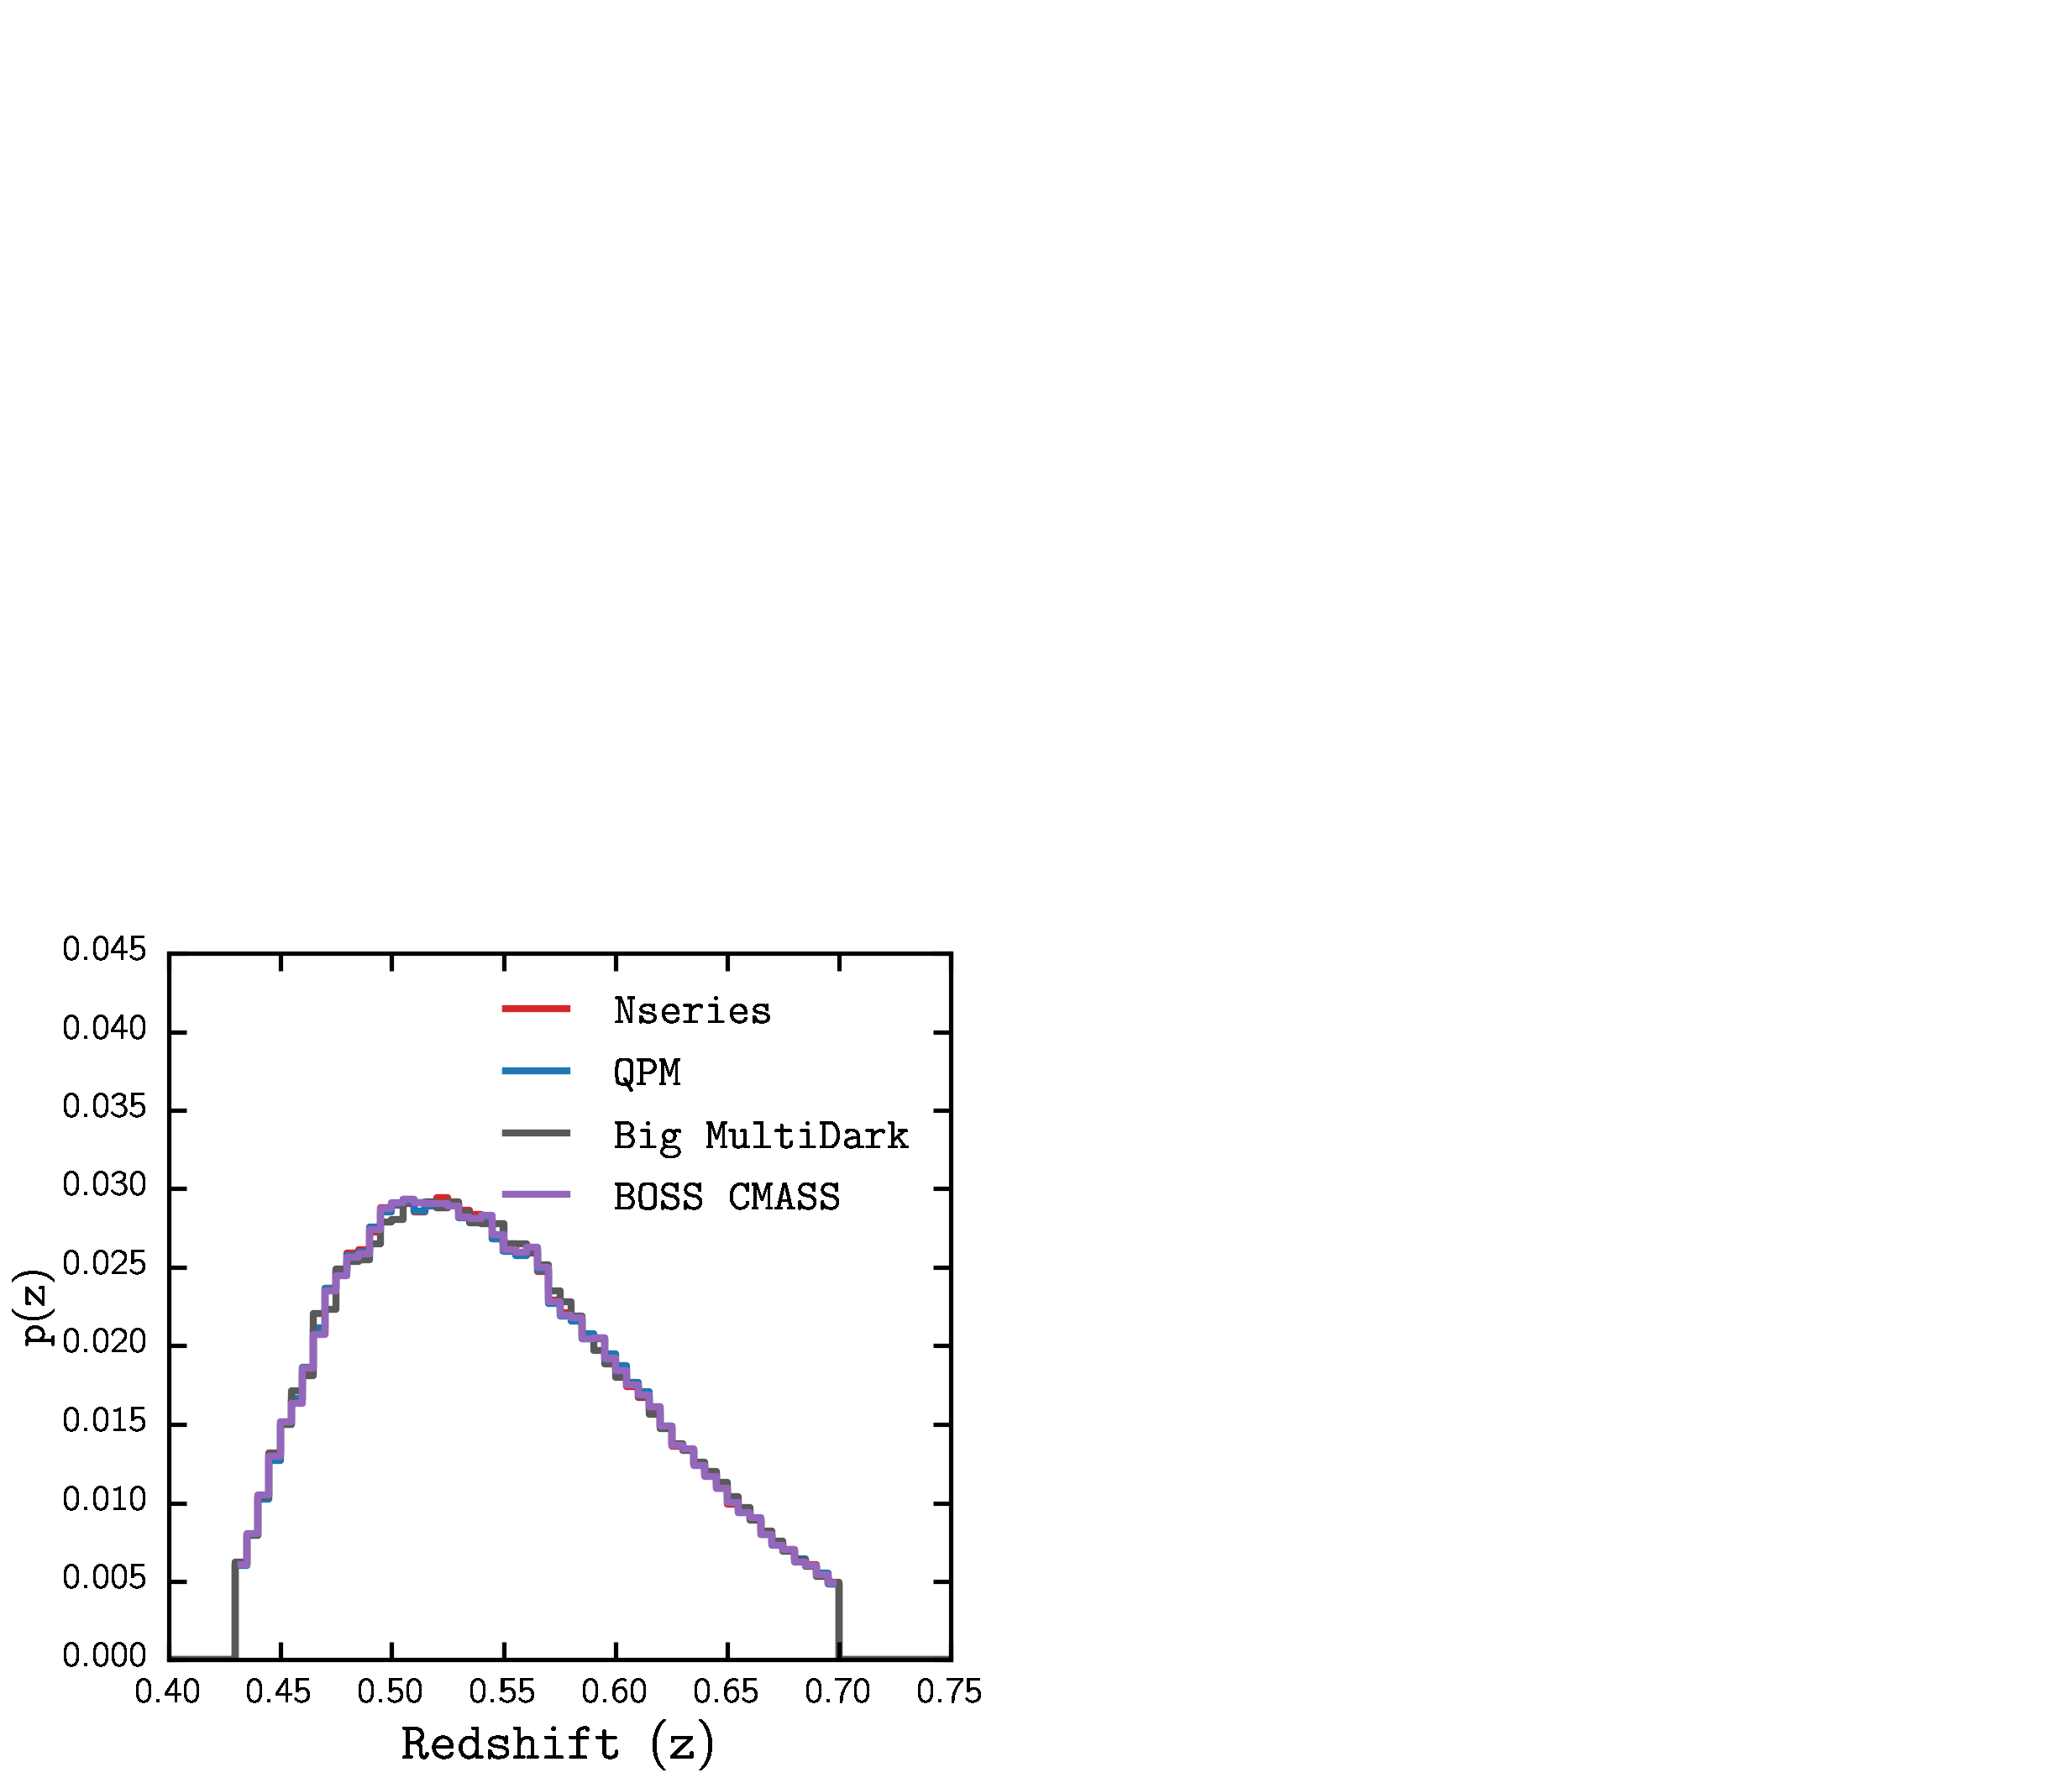
\includegraphics[width=1.\textwidth]{figs/fc/mock_catalog_z_dist.pdf} 
\caption{Normalized galaxy redshift distribution of the Nseries (\nseriescolor), 
QPM (\qpmcolor), and BigMultiDark (\bmdcolor) mock catalogs. The 
normalized redshift distribution of BOSS DR12 CMASS sample galaxies 
is also plotted (\cmasscolor). Each of the distributions were computed
with a bin size of $\Delta z = 0.025$. All of the mock catalogs used 
in this work closely trace the BOSS CMASS redshift distribution.}
\label{fig:zdist}
\end{center}
\end{figure}

Effects of fiber collisions must be understood and interpreted in conjunction 
with the other systematic effects. Therefore, in this paper, we use Quick 
Particle Mesh (\citealt{White:2014aa}), Nseries (Tinker et al. in prep), and 
the BigMultiDark (\citealt{Rodriguez-Torres:2015aa}) mock catalogs, which 
have already been extensively used in interpreting clustering results for  
BOSS and are generated through different prescriptions. Therefore they 
provide a robust sets of data to measure the effects of fiber collisions and 
to test our correction methods. 

The QPM mock galaxy catalogs uses a ``quick particle mesh" method, which uses 
a low resolution particle-mesh N-body solver, with a resolution of 
$2\;\mathrm{Mpc}/h$, to evolve particles within a 
periodic simulation volume. The particles are assigned halo masses in order 
to match the halo mass function and large-scale bias of halos of high resolution 
simulations. Afterwards the HOD parameterization of \cite{Tinker:2012aa} is 
used to populate the halos. The mock galaxy sample is then trimmed to the 
BOSS CMASS survey footprint, downsampled based on angular sky completeness 
(sector completeness) and radial selection. Furthermore, QPM mocks model the 
fiber collisions of the BOSS CMASS sample ($62"$). QPM uses the following 
$\Lambda$CDM cosmology: $\Omega_\mathrm{m} = 0.29$, $\Omega_\Lambda = 0.71$, 
$\sigma_8 = 0.8$, $n_\mathrm{s} = 0.97$ and $h=0.7$. We use 100 realizations 
of the QPM catalog. For a detailed description of the QPM galaxy mock catalogs 
we refer readers to \cite{White:2014aa}. 

Next, the Nseries mock catalogs are created from a series of high-resolution 
N-body simulations. Each mock has the same angular selection function as the 
North Galactic Cap region of the BOSS DR12 large-scale structure sample for 
CMASS galaxies (\citealt{Cuesta:2016aa}). They also reproduce the 
redshift distribution of the BOSS CMASS sample. The Nseries mock catalogs are 
created from seven independent N-body simulations, each of the same cosmology. 
Each simulation box is $2.5\;\mathrm{Gpc}/h$ per side with cosmology: 
$\Omega_\mathrm{m} = 0.286$, $\Omega_\Lambda = 0.714$, $\sigma_8 = 0.82$,
$n_\mathrm{s} = 0.96$ and $h=0.7$. Out of these Nseries box simulations, the 
three orthogonal projections of each box is used to create $84$ mocks.
Each of the cut-out mocks is then passed through the same fiber assignment 
code as the actual BOSS data using the distribution of plates in BOSS. 
Thus, the angular variation of fiber collisions faithfully reproduces 
that of the data, with $\sim 5\%$ of the targets without fibers due to close 
neighbors in regions of the footprint only covered by one tile. 

%%%%%%%%%%%%%%%%%%%%%%%%%%%%%%%%%%%%%%%%%%%%%%%%%%%%%%%%%%%%%%%%%%%%%%%%%%%%%%
% P(k) plot for mocks and BOSS --------------------------------------------------
\begin{figure*}
\begin{center}
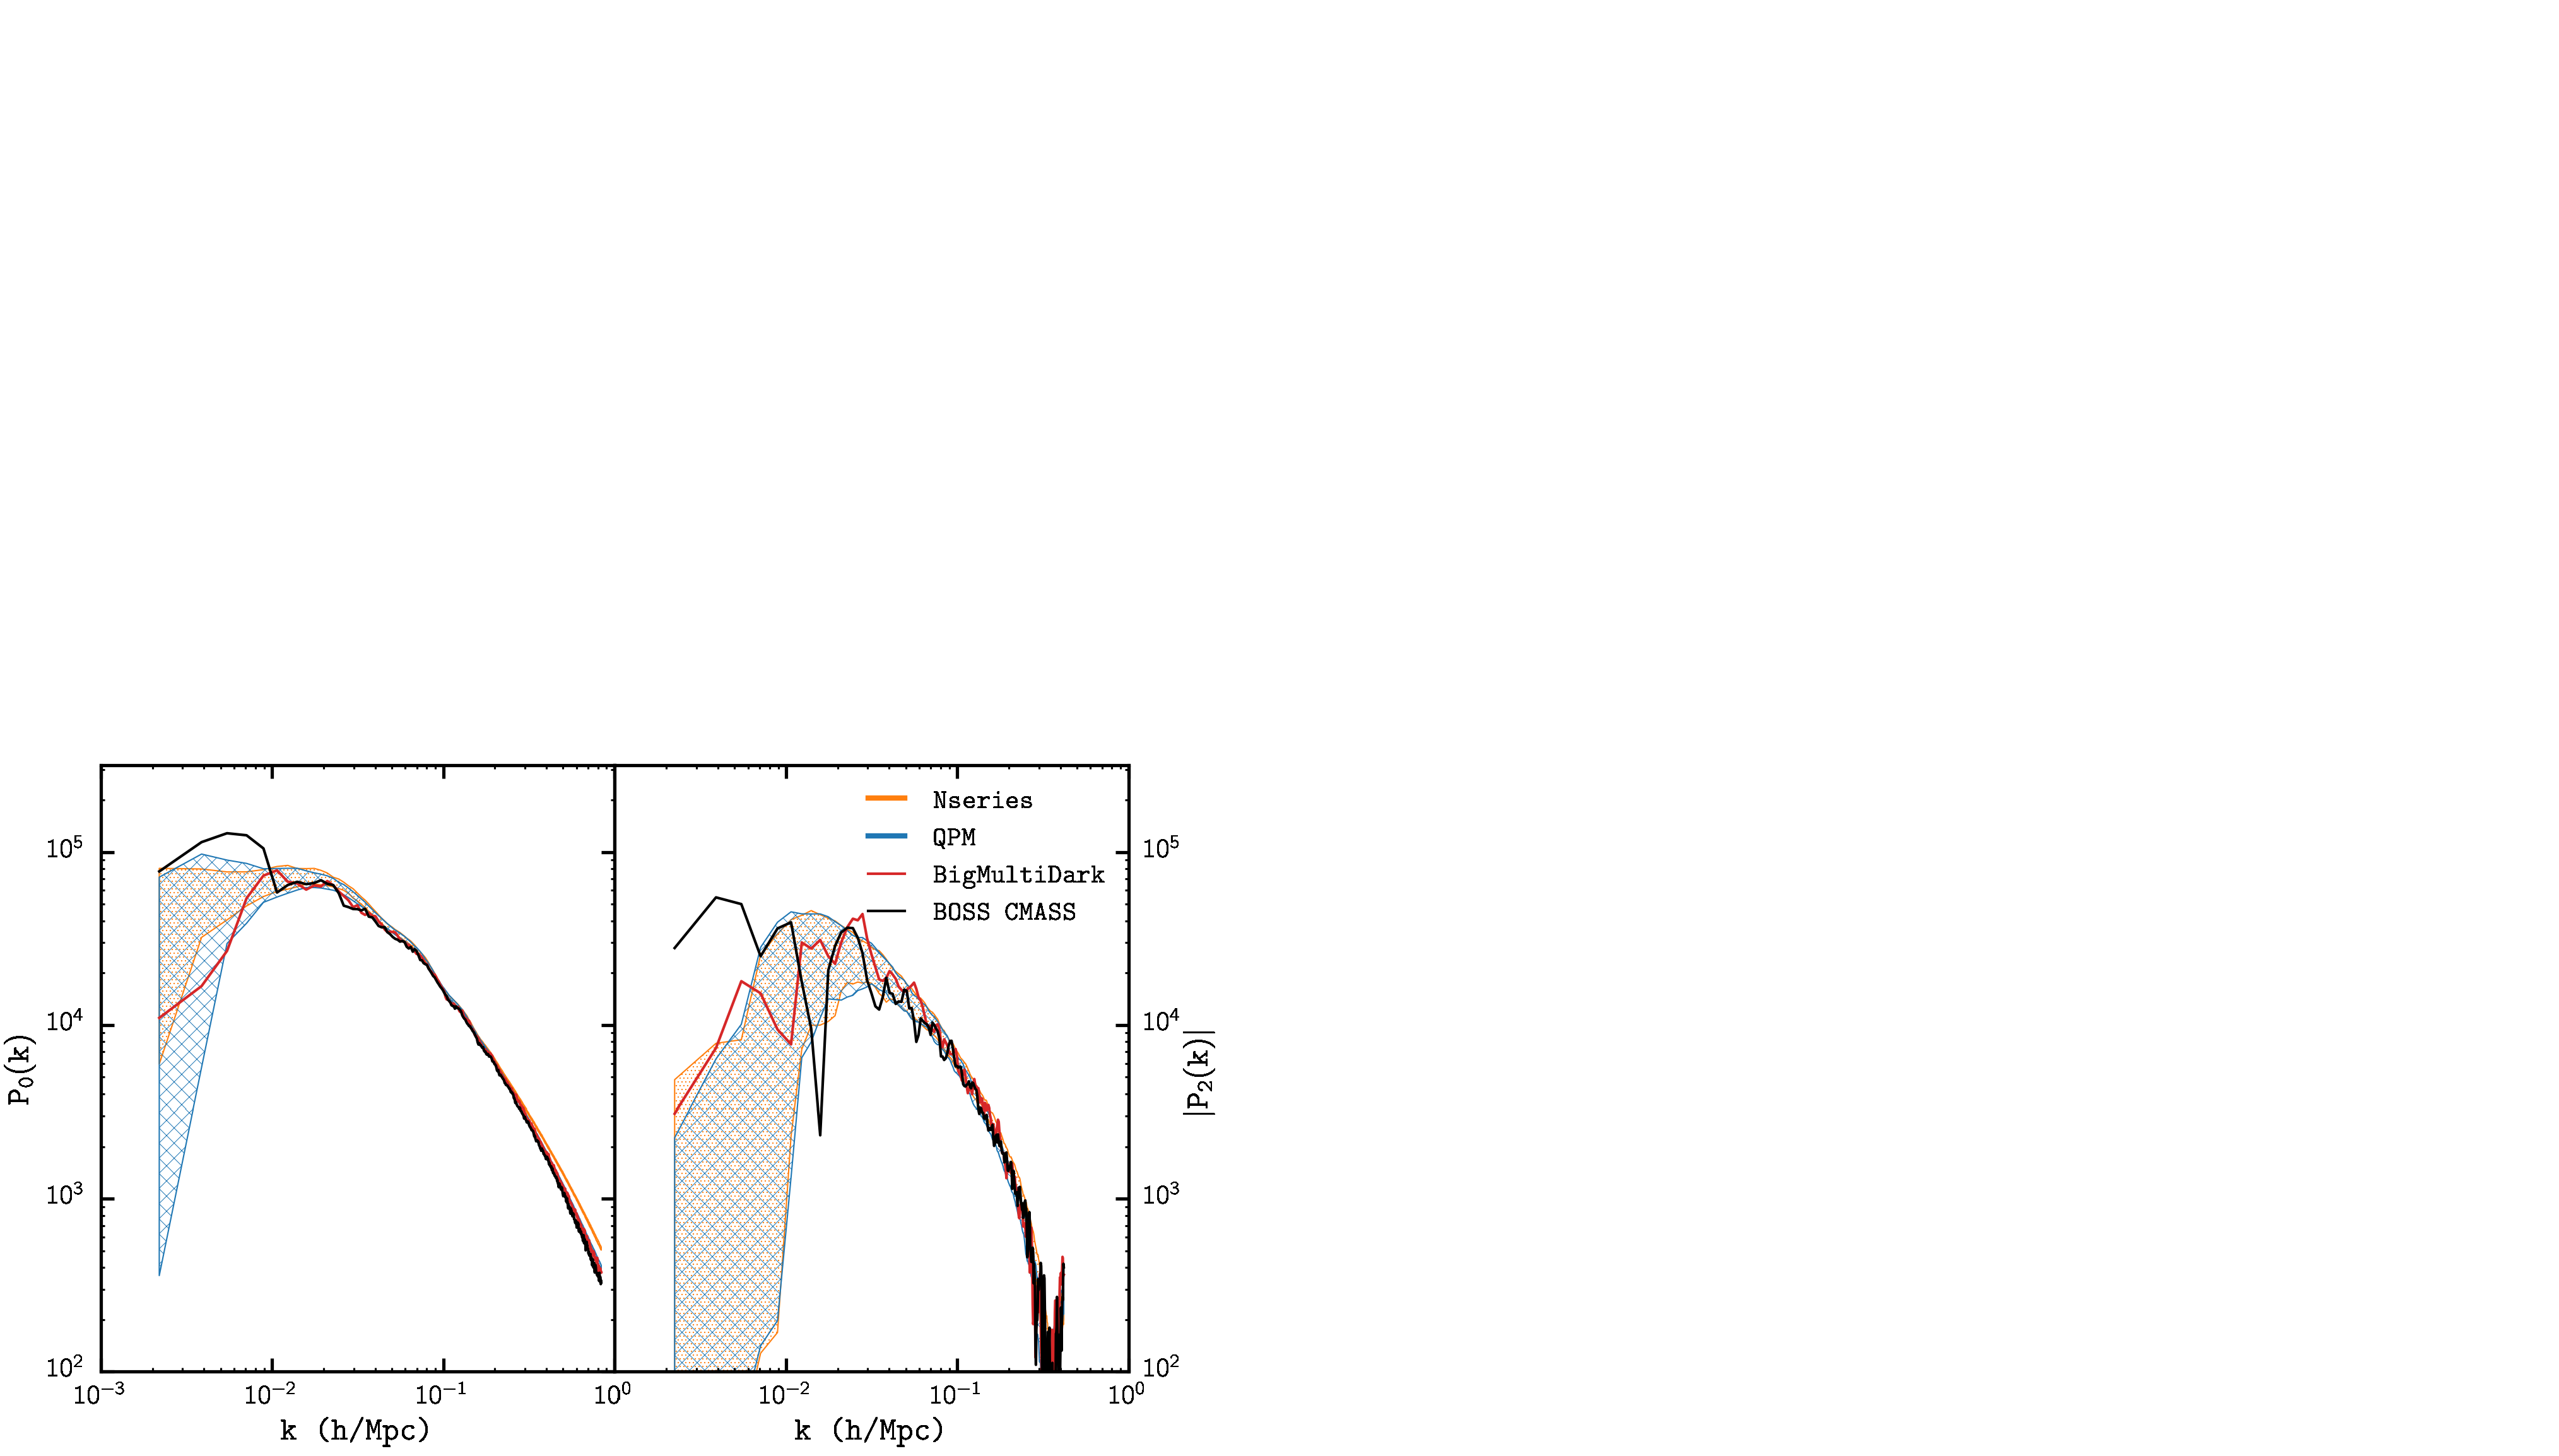
\includegraphics[width=1.\textwidth]{figs/fc/mock_catalog_Plk.pdf} 
\caption{
Power spectrum monopole $P_0(k)$ and 
quadrupole $|P_2(k)|$ measurements for the Nseries (\nseriescolor), 
QPM (\qpmcolor), and BigMultiDark (\bmdcolor) mock catalogs 
(Section \ref{sec:catalog}). The $P_l(k)$ measurements 
for the Nseries and QPM mock catalogs are averaged over the
multiple mock realizations and the width of the power spectra represents 
the sample variance ($\sigma_l(k)$; Eq.~\ref{eq:pk_var}) of the realizations. 
For the quadrupole, we plot the $|{P_2(k)}|$ instead of 
${P_2(k)}$ because the measurement becomes negative for 
$k \gtrsim 0.35\;h/\mathrm{Mpc}$. For comparison, we also include the monopole and 
quadrupole power spectra of the BOSS DR12 CMASS sample, which are calculated 
using the same estimator but with statistical weights described in Eq.~(\ref{eq:weight}). 
While fiber collisions are inevitably included in the BOSS CMASS power spectra, 
they are {\it not} yet applied to the mock catalogs power spectra measurements above. } 
\label{fig:mockpk}
\end{center}
\end{figure*}
%%%%%%%%%%%%%%%%%%%%%%%%%%%%%%%%%%%%%%%%%%%%%%%%%%%%%%%%%%%%%%%%%%%%%%%%%%%%%%

Finally the BigMultiDark galaxy mock catalog is generated using the 
BigMultiDark Planck (BigMDPL), one of the MultiDark3 N-body simulations 
(\citealt{Klypin:2014aa}). BigMDPL uses a GADGET-2 code (\citealt{Springel:2005ab})
in a cubic box of $2.5\;h^{-1}\mathrm{Gpc}$ sides with $3840^3$ dark matter 
particles and a mass resolution of $2.4\times 10^{10} h^{-1}M_\odot$. 
As the name suggests, BigMDPL uses Planck cosmological parameters in a flat $\Lambda$CDM cosmology: 
$\Omega_m = 0.307$, $\Omega_B = 0.048$, $\Omega_\lambda = 0.693$, $\sigma_8 = 0.829$, 
$n_s = 0.96$ and $h = 0.678$. 

From the BigMDPL N-body simulation, \cite{Rodriguez-Torres:2015aa} uses 
the $\mathtt{RockStar}$ (Robust Overdensity Calculation using K-Space Topologically 
Adaptive Refinement) halo finder (\citealt{Behroozi:2013aa}) to obtain 
a dark matter halo catalog. Afterwards, they use the 
SUrvey GenerAtoR code ($\mathtt{SUGAR}$) to generate a galaxy catalog from the halo 
catalog. $\mathtt{SUGAR}$ uses halo abundance matching with an intrinsic scatter 
on the stellar mass function of the Portsmouth SED-fit DR12 stellar mass
catalog (\citealt{Maraston:2013aa}) to populate the dark matter halos with  
galaxies. \cite{Rodriguez-Torres:2015aa} then model fiber collisions using 
\cite{Guo:2012aa} in order to reproduce the effect of fiber collisions on 
the observed BOSS galaxies. For any further details on the BigMultiDark 
galaxy mock catalog, we refer readers to \cite{Rodriguez-Torres:2015aa}.

In Figure \ref{fig:zdist}, we plot the normalized redshift distribution of the 
Nseries (\nseriescolor), QPM (\qpmcolor), and BigMultiDark (\bmdcolor) 
mock catalogs along with the redshift distribution of the BOSS DR12 
CMASS sample galaxies. All of these mock catalogs were constructed
for the BOSS analysis and their redshift distributions closely 
trace the observed BOSS distribution.


%%%%%%%%%%%%%%%%%%%%%%%%%%%%%%%%%%%%%%%%%%%%%%%%%%%%%%%%%%%%%%%%%%%%%%%%%%%%%%
% Powerspectrum Estimator
%%%%%%%%%%%%%%%%%%%%%%%%%%%%%%%%%%%%%%%%%%%%%%%%%%%%%%%%%%%%%%%%%%%%%%%%%%%%%%
\subsection{Power Spectrum Estimator} \label{sec:pk_est}
In this paper, out of the many possible clustering measurements, we focus on the 
galaxy power spectrum and its monopole and quadrupole in redshift space. 
Throughout the paper, unless specified, when we measure the 
power spectrum we use the estimator described in \cite{Scoccimarro:2015aa}, 
which accounts for radial redshift space distortions (see also \citealt{Bianchi:2015aa}). 
In this estimator, galaxies are interpolated and Fast Fourier 
transformed as discussed in \cite{Sefusatti:2016aa}. 
Since the algorithm is efficient, it makes power spectrum computations 
for large number of mock realizations tractable.

To summarize the method, we calculate the 
monopole component of the power spectrum using: 
\begin{equation}\label{eq:roman_p0k}
\widehat{P_0}(k) = \frac{1}{I_{22}} \left[ \int \frac{d\Omega_k}{4 \pi} |F_0({\bf k})|^2 - N_0 \right]
\end{equation}
where 
\begin{equation}
F_0({\bf k}) = \left( \sum_{j = 1}^{N_g} - \alpha \sum_{j=1}^{N_r} \right) w_j\;e^{i {\bf k}\cdot{\bf x}_j}
\end{equation}
with normalization constant
\begin{equation} \label{eq:i22}
I_{22} = \alpha \sum^{N_r}_{j=1} \bar{n}({\bf x}_j)w_j^2
\end{equation}
and shot noise term following from the estimator is \citep{Scoccimarro:2015aa}
\begin{equation} \label{eq:roman_shotnoise}
N_0 = \left( \sum_{j = 1}^{N_g} + \alpha^2 \sum_{j=1}^{N_r} \right) w_j^2, 
\end{equation}
which represents the constant shot noise contribution to the power due to 
the discrete density field of our galaxies and random catalog. Here $\alpha$ is the ratio of the 
number of galaxies ($N_g$) over the number of synthetic random galaxies 
($N_r$), $\bar{n}({\bf x})$ is the mean density of the galaxies at position 
${\bf x}$, and $w_j$ is weight of each object, which includes the minimum 
variance weight from \cite{Feldman:1994aa}: 
\begin{equation}
w_{\mathrm{FKP}} ({\bf x}_j) = \frac{1}{1+\bar{n}({\bf x}_j) P_0}
\end{equation}
where $P_0$ is the power spectrum amplitude at which the error is minimized. 
We use $P_0 = 20000\; \mathrm{Mpc}^3/h^3$ for our analysis, which corresponds 
to $k \sim 0.1\; h/\mathrm{Mpc}$. We note that the shot noise term in 
Eq.~(\ref{eq:roman_shotnoise}) differs from the standard shot noise term from
\cite{Feldman:1994aa}. The difference between various shot noise expressions used in the literature  
will be discussed in detail in Section \ref{sec:shotnoise}. 

For the quadrupole, we have 
\begin{equation}\label{eq:roman_p2k}
\widehat{P_2}(k) = \frac{5}{I_{22}} \int \frac{d\Omega_k}{4 \pi} F_2({\bf k}) F_0^*({\bf k})
\end{equation}
where 
\begin{equation}
F_2({\bf k}) = \frac{3}{2}\hat{k}_a\hat{k}_b Q^{ab}({\bf k}) - \frac{1}{2} F_0({\bf k})
\end{equation}
with 
\begin{equation}
Q^{ab}({\bf k}) = \left( \sum_{j = 1}^{N_g} - \alpha \sum_{j=1}^{N_r} \right) \hat{x}_j^a\hat{x}_j^b w_j \;e^{i {\bf k}\cdot{\bf x}_j}
\end{equation}

In Figure \ref{fig:mockpk}, we plot the  power spectrum monopole and quadrupole, ${P_0(k)}$ 
and $|{P_2(k)}|$, measured using Eq.~(\ref{eq:roman_p0k}) and Eq.~(\ref{eq:roman_p2k}), respectively, for the Nseries, QPM, and BigMultiDark 
mock catalogs. We plot $|{P_2(K)}|$ because the power spectrum quadruple 
becomes negative for $k \gtrsim 0.35\;h/\mathrm{Mpc}$. ${P_0(k)}$ and
$|{P_2(k)}|$ are averaged over the $84$ and $100$ realizations for
Nseries and QPM. We note that fiber collisions are not applied to these mock 
catalogs. Without fiber collisions, the weights of the objects are equivalent 
to the FKP weights, $w_j = w_{j,\mathrm{FKP}}$. 

We also plot the $P_0(k)$ and $P_2(k)$ of the BOSS Data Release 12 CMASS 
data (\cmasscolor) in Figure \ref{fig:mockpk}. For BOSS DR12 CMASS, 
systematic weights are assigned to the galaxies in order to account for 
sector completeness, redshift failures, and fiber collisions. Each galaxy 
has a statistical weight determined by, 
\begin{equation} \label{eq:weight}
w_{j, \mathrm{tot}} = w_{j, \mathrm{sys}} (w_{j, \mathrm{rf}} + w_{j, \mathrm{fc}} -1), 
\end{equation} 
(\citealt{Anderson:2012aa, Ross:2012aa, Beutler:2014aa}), which are included in the 
final object weight $w_j$ along with $w_{j, \mathrm{FKP}}$. In this formula, $w_{j,\mathrm{rf}}$ is a weight that accounts for redshift failures and $w_{j,\mathrm{fc}}$
is the fiber collision weight determined by the nearest angular neighbor method, which we
later discuss in Section \ref{sec:fc_pk}. The statistical 
weights are also included in $\alpha = \sum_{j=1}^{N_g} w_\mathrm{tot} / N_r$. 
We note that fiber collisions are inevitably included in the CMASS $P_l(k)$.
However they are not yet included in the $P_l(k)$ of the mock catalogs in Figure \ref{fig:mockpk}.

For the mock catalogs with multiple realizations (QPM and Nseries), we 
compute the sample variance of the power spectrum
\begin{equation} \label{eq:pk_var}
\sigma_l (k)= \sqrt{\frac{1}{N_\mathrm{mocks}-1} \sum\limits_{i=1}^{N_\mathrm{mocks}} (P^i_l(k)- \langle{P_l(k)}\rangle)^2 \ }. 
\end{equation}
$N_\mathrm{mock}$ is the number of mock realizations (84 for Nseries and 100 for 
QPM) and $P^i_l(k)$ is the power spectrum for each realization. $\sigma_l(k)$ is 
represented in Figure \ref{fig:mockpk} by the width of the shaded regions. 
%%%%%%%%%%%%%%%%%%%%%%%%%%%%%%%%%%%%%%%%%%%%%%%%%%%%%%%%%%%%%%%%%%%%%%%%%%%%%%
% NN P_l(k) Residual figures 
%%%%%%%%%%%%%%%%%%%%%%%%%%%%%%%%%%%%%%%%%%%%%%%%%%%%%%%%%%%%%%%%%%%%%%%%%%%%%%
\begin{figure*}
\begin{center}
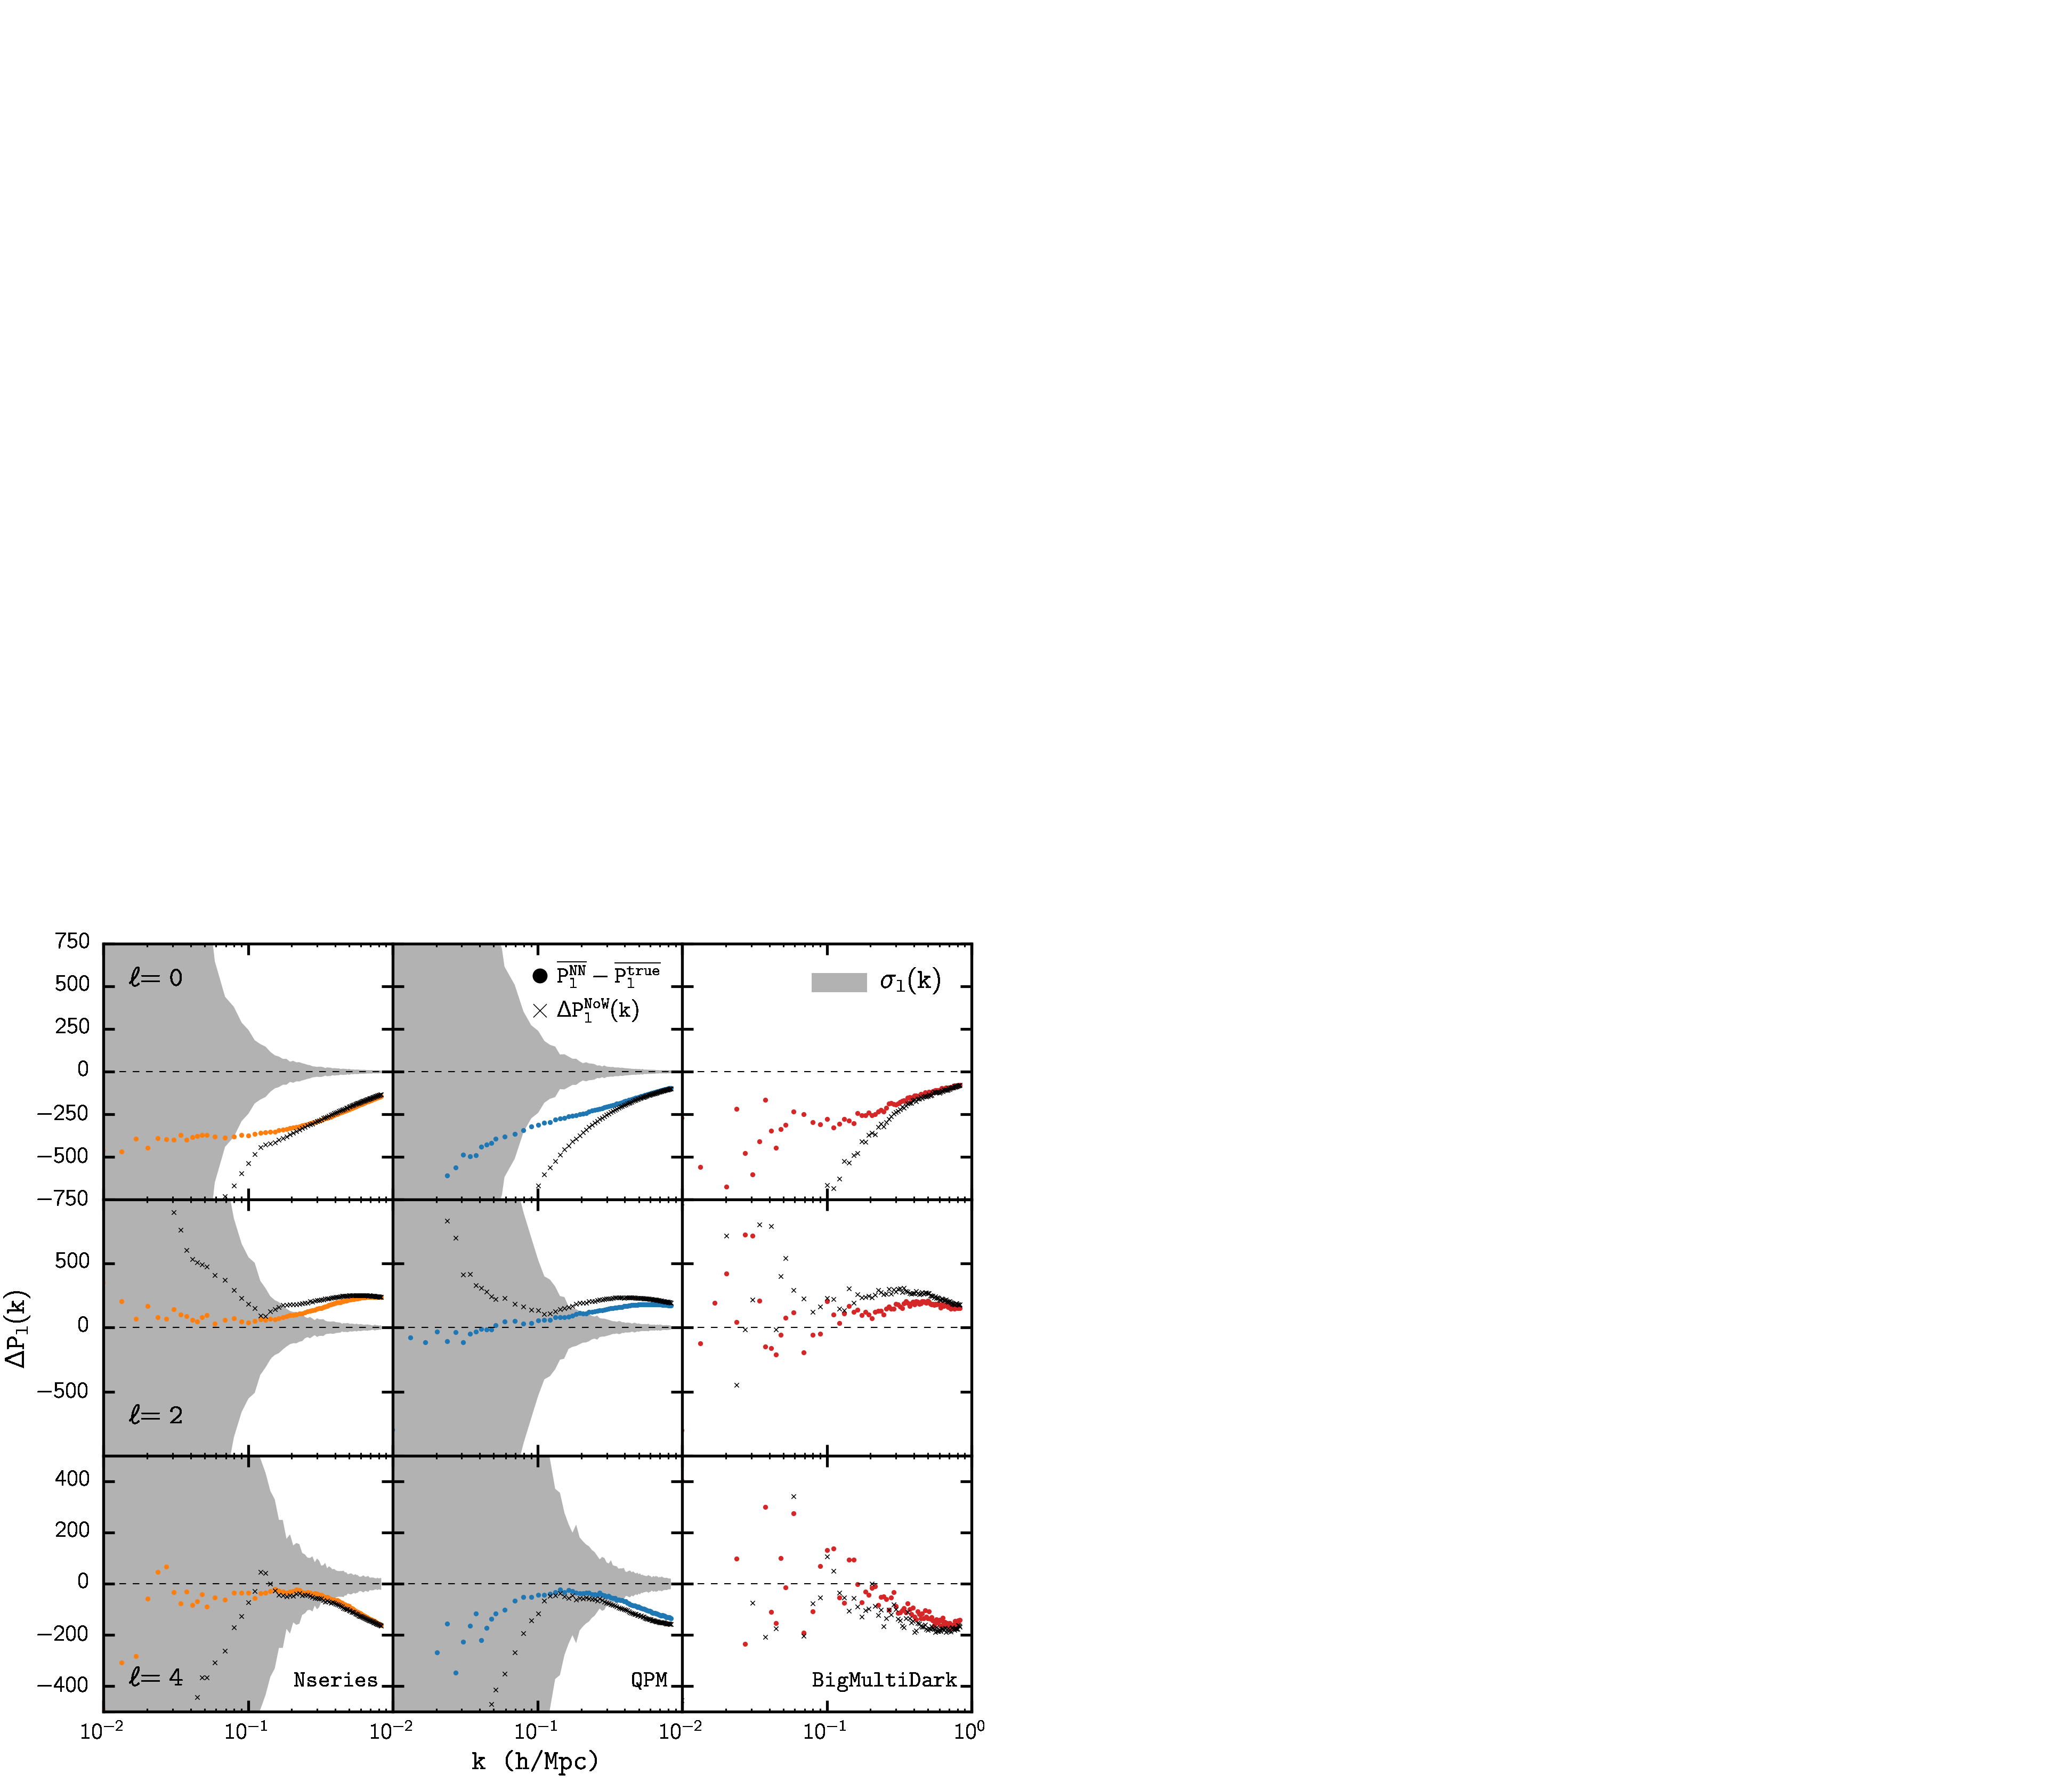
\includegraphics[width=1.\textwidth]{figs/fc/mock_catalog_NN_true_P024k_resid_rebin6x.pdf} 
\caption{The fiber collision power spectrum residual, 
$(P_l^\mathrm{NN}-P_l^\mathrm{true})$ 
(Section \ref{sec:fc_pk}), for the monopole (top), quadrupole 
(middle), and hexadecapole (bottom) of the Nseries (left), QPM (middle), and 
BigMultiDark (right) mock catalogs. For the Nseries and QPM mocks, 
we plot the sample variances $\sigma_l(k)$ (grey shaded region) of 
$P_l^\mathrm{true}(k)$ for comparison. The power spectrum residual for the 
NN method is an improvement over the residual with no correction 
($\Delta P_l^\mathrm{NoW}(k)$; x) at most scales probed. 
However, we highlight that at $k > 0.1 \;h/\mathrm{Mpc}$ and 
$k > 0.2\;h/\mathrm{Mpc}$, for the monopole and quadrupole 
respectively, the residuals from fiber collision surpass the sample 
variance. 
At smaller scales, NN method does not sufficiently account for 
the effects of fiber collisions in $P_l(k)$ measurements.}
\label{fig:fc_pk}
\end{center}
\end{figure*}

\begin{figure}
\begin{center}
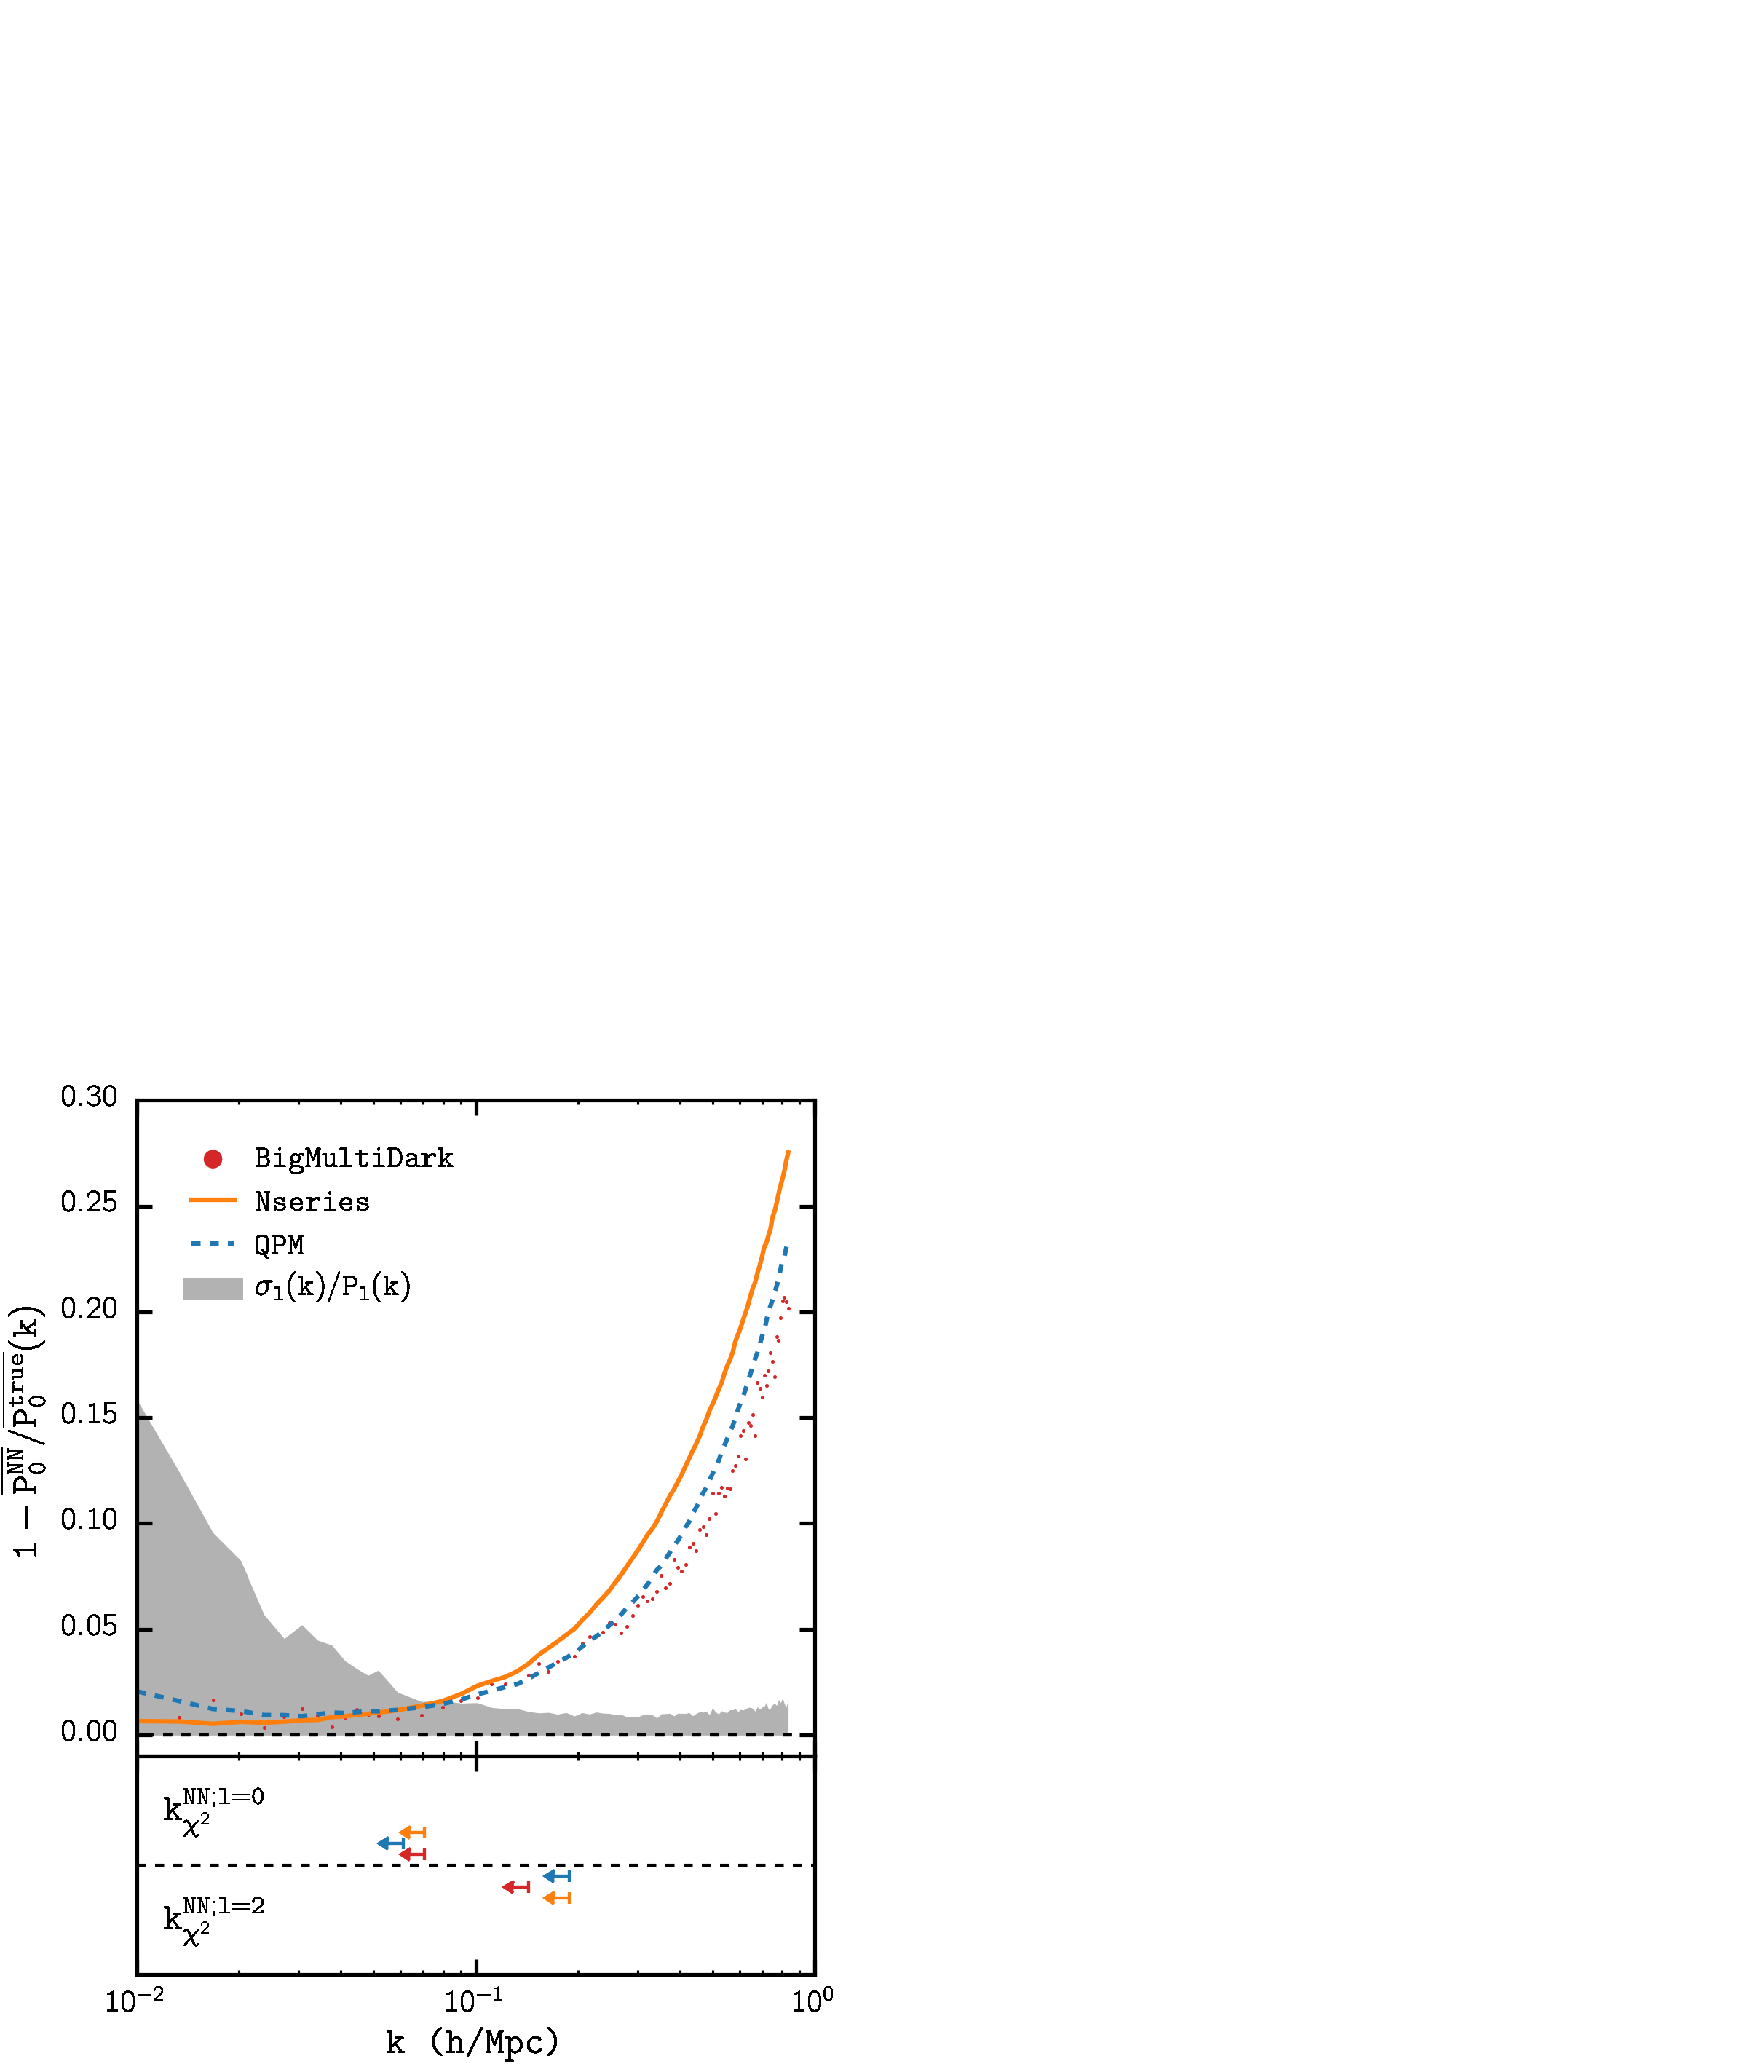
\includegraphics[width=1.\textwidth]{figs/fc/mock_catalog_NN_true_P0k_norm_resid_rebin6x.pdf} 
\caption{{\it Top Panel}: The normalized residuals, 
$1 - \overline{P_0^\mathrm{NN}}/\overline{P_0^\mathrm{true}}(k)$, 
of the NN method for the Nseries (\nseriescolor), 
QPM (\qpmcolor), and BigMultiDark (\bmdcolor) power spectrum monopole. 
We also plot the normalized sample variance $\sigma_0(k) / P_0(k)$ 
(gray shaded region) of the Nseries mocks for comparison.
The QPM $\sigma_0(k) / P_0(k)$ is effectively the same as the Nseries 
$\sigma_0(k)/P_0(k)$, so we do not included in the figure. 
The comparison reveals that the effect of fiber collisions not only 
biases the power spectrum beyond sample variance at $k \gtrsim 0.1 \;h/\mathrm{Mpc}$, 
but that the effect increases relative to sample variance at smaller scales. At 
$k = 0.2\;h/\mathrm{Mpc}$,  
the normalized residual is greater than $4$ times the normalized sample variance.
{\it Bottom Panel}: We mark $k_{\chi^2}$ where $\Delta \chi^2(k_{\chi^2}) = 1$ (Eq.~\ref{eq:chisquared}) for the NN method. $k^\mathrm{NN}_{\chi^2}$ is a conservative 
scale limit of the NN method. Arrows above the dashed 
line mark $k_{\chi^2}$ for the monopole while the arrows below the dashed line mark
$k_{\chi^2}$ for the quadrupole. The color of the arrows indicate the mock catalog: 
Nseries (\nseriescolor), QPM (\qpmcolor), and BigMultiDark (\bmdcolor). Averaged
over the three mock catalogs, we get $k^\mathrm{NN}_{\chi^2} = 0.068$ and $0.17 \;h/\mathrm{Mpc}$.
for the monopole and quadrupole respectively.}
\label{fig:NN_norm_resid}
\end{center}
\end{figure}
%%%%%%%%%%%%%%%%%%%%%%%%%%%%%%%%%%%%%%%%%%%%%%%%%%%%%%%%%%%%%%%%%%%%%%%%%%%%%%
% fiber collision Correction Method
%%%%%%%%%%%%%%%%%%%%%%%%%%%%%%%%%%%%%%%%%%%%%%%%%%%%%%%%%%%%%%%%%%%%%%%%%%%%%%
\section{Fiber Collision Methods} \label{sec:fc_corr}
%%%%%%%%%%%%%%%%%%%%%%%%%%%%%%%%%%%%%%%%%%%%%%%%%%%%%%%%%%%%%%%%%%%%%%%%%%%%%%
% Effects of Fiber Collision on the Power Spectrum 
%%%%%%%%%%%%%%%%%%%%%%%%%%%%%%%%%%%%%%%%%%%%%%%%%%%%%%%%%%%%%%%%%%%%%%%%%%%%%%
\subsection{Nearest Angular Neighbor Method (NN)} \label{sec:fc_pk}
A common approach to accounting for fiber collisions in clustering measurements has been 
to use the nearest angular neighbor method (\citealt{Zehavi:2002aa, Zehavi:2005aa, 
Berlind:2006aa, Zehavi:2011aa, Anderson:2012aa}),
hereafter NN method. For galaxies without resolved spectroscopic redshifts due to fiber 
collisions, the entire statistical weight of the galaxy is assigned to its nearest angular 
neighbor with resolved redshift. 
According to \cite{Zehavi:2002aa}, this method 
effectively assumes that all galaxies within the angular fiber collision scale ($< 62"$ for BOSS) are correlated with one another. 
In the context of the halo model, the NN method assumes that 
galaxies within the fiber collision angular scale reside in the same halo 
so displacing one of the galaxies and placing it on top of the other does 
not significantly impact clustering statistics. % change it so that it sounds like we're quoting other people's work.
This is a reasonable assumption  
for the 2PCF and the power spectrum on scales far greater than fiber collisions.  

One consequence of this method is that galaxies coincidentally within the angular 
fiber collision scale (hereafter referred to as ``chance 
alignments") are incorrectly assumed to be gravitationally correlated and 
within the same halo. So when the statistical weight of the collided galaxy
is added to its nearest angular neighbor, the collided galaxy is in fact 
displaced significantly from its true radial position. This displacement can even 
be on the scale of the survey depth, which corresponds to $\sim500\;\mathrm{Mpc}$
for BOSS. Furthermore, even for fiber collided galaxies that reside in the 
same gravitationally bound structures such as groups or clusters, up-weighting 
the nearest neighbor disregards the line-of-sight displacements within these 
structures. 

To precisely quantify the effect of fiber collisions on the power spectrum, 
we compare the power spectrum measurements of the NN weighted fiber collided
mock catalogs $P_l^\mathrm{NN}$ to the power spectrum measurements of 
the mock catalogs without fiber collisions, the ``true'' power spectrum 
$P_l^\mathrm{true}$. Specifically, in Figure \ref{fig:fc_pk}, we 
plot the power spectrum residual $(P_l^\mathrm{NN} - P_l^\mathrm{true})$ as a function of $k$. 
The power spectrum estimators Eq.~(\ref{eq:roman_p0k}) and~(\ref{eq:roman_p2k})  
are used to calculate the monopole (top) and quadrupole (center) respectively. 
We include measurements of the sample 
variance, $\sigma_l(k)$, for the Nseries and QPM mock catalogs (Eq.~\ref{eq:pk_var}). 
We also include the power spectrum residual $\Delta P_l^\mathrm{NoW}(k) = 
P_l^\mathrm{NoW}(k) - P_l^\mathrm{true}(k)$ (dashed), where $P_l^\mathrm{NoW}(k)$ is the 
power spectrum of the fiber collided mock catalogs with {\em no} NN weights,
with the collided galaxies removed from the sample. 
In this paper we focus on the monopole and quadrupole, 
however for reference, we also include the effect of fiber collisions on the power spectrum hexadecapole (bottom).

As both $P_l(k)$ and $\sigma_l(k)$ vary significantly over the probed $k$ range, the significance 
of the discrepancies between $P^\mathrm{NN}_l(k)$ and $P^\mathrm{true}_l(k)$ 
are not adequately portrayed in Figure \ref{fig:fc_pk}, especially for the monopole. 
Therefore, to compare $P_0^\mathrm{NN}$ and $P_0^\mathrm{true}$ over a wide $k$ 
range and to especially highlight the discrepancies at small scales, in 
Figure \ref{fig:NN_norm_resid}, we compare the normalized monopole residuals, 
$1 - P_0^\mathrm{NN}/P_0^\mathrm{true}$, to the normalized sample variance,
$\sigma_0(k)/P_0^\mathrm{true}$. 
% and plot the normalized residual rather than the  $P_l^\mathrm{NN} - P_l^\mathrm{true}$  because $P_l(k)$ spans over three orders of magnitude over the $k$ range probed in our measurement. For instance, although $P_l^\mathrm{NN} - P_l^\mathrm{true}$  decreases at small scales, $P_l(k)$ decreases as well; so as the normalized residuals  highlight, the discrepancy is more significant at small scales.  

For the monopole, Figure \ref{fig:fc_pk} demonstrates that while the 
NN method (circles) provides an overall improvement over applying no correction (crosses)
at most scales, fiber collisions still significantly bias the corrected 
power spectrum at all scales. The effect also has a significant $k$ 
dependence, which implies that an adjusted 
constant shot noise term alone is insufficient in accounting for the deviation. 
Even at $k \approx 0.1\;h/\mathrm{Mpc}$, the effect of 
fiber collisions in the NN method alarmingly surpasses sample variance. 
While the amplitude of the residual decreases as $k$ increases, Figure
\ref{fig:NN_norm_resid} reveals that as a fraction of 
$P_0^\mathrm{true}(k)$, the discrepancy is in fact increasing. 
In other words, the NN method becomes less effective at correcting for 
fiber collisions on smaller scales, as expected. At the smallest scales probed 
($k = 0.83\;h/\mathrm{Mpc}$), the $P_0^\mathrm{NN}(k)$ underestimates the 
true power spectrum monopole by over $20\%$. 
%More importantly, at the scale limits of 
%current power specturm monopole models ($k\sim 0.3\;h/\mathrm{Mpc}$; 
%\todo{CITECITE}), the average normalized residual of the NN method 
%is $9.8\%$, which is over six times the normalized cosmic variance, $1.5\%$. 

For the quadrupole, the NN method improves the power spectrum residuals over 
no correction. However, even with the NN method, the effect of fiber collisions begins 
to significantly grow at $k=0.1\;h/\mathrm{Mpc}$ and becomes comparable to 
the sample variance at $k \sim 0.2\;h/\mathrm{Mpc}$. For $k > 0.2\;h/\mathrm{Mpc}$, 
the effect continues to increase and quickly overtakes the decreasing 
sample variance. At the smallest scales measured ($k = 0.83 \;h/\mathrm{Mpc}$) the 
residual is over eight times the sample variance.

Recently power spectrum analyses have measured the power spectrum using a wide range of 
$k$ bins: for example, \cite{Anderson:2012aa} use $\Delta k = 0.04 \;h/\mathrm{Mpc}$ and \cite{Beutler:2014aa} and \cite{Grieb:2016aa} use 
$\Delta k = 0.005\;h/\mathrm{Mpc}$. Here, we use $\Delta k = 0.01\;h/\mathrm{Mpc}$, 
which is within this general range, in agreement with~\cite{Beutler:2016aa} and \cite{Gil-Marin:2016ab}. Sample variance measured with larger $\Delta k$ 
is smaller; so a straight comparison in Figure \ref{fig:fc_pk} between the power spectrum residuals (symbols) 
and the sample variance (shaded region) has a significant dependence on 
the choice of $\Delta k$. What is independent of binning is a cumulative $\chi^2$ as a function of $k$, and thus we define a $k$ scale limit $k_{\chi^2}$  
so that $\Delta  \chi^2(k_{\chi^2}) = 1$, where 
\beq \label{eq:chisquared}
\Delta \chi^2(k') = \sum\limits_{i,j < N_k} 
\left[P^\mathrm{NN}_{l,i} - P^\mathrm{true}_{l,i}\right] C^{-1}_{l;\; i,j}
\left[P^\mathrm{NN}_{l,j} - P^\mathrm{true}_{l,j}\right]
\eeq
where $N_k$ is the number of bins where $k < k'$ and $C^{-1}_{l; i,j}$ are the elements of the
inverse covariance matrix for $P_l^\mathrm{true}(k)$. The elements of the covariance matrix 
$\mathbf{C}_l$ are computed as 
\beq
\mathrm{C}_{l;\; i,j} = \frac{1}{N_{\mathrm{mocks}}-1}\sum_{k=1}^{N_{\mathrm{mocks}}}
\Big[P^{(k)}_{l;\;i}-\overline{P}_{l;\;i}\Big]
\Big[P^{(k)}_{l;\;j}-\overline{P}_{l;\;j}\Big]
\nonumber
\eeq
for the Nseries and QPM mocks. For BigMD, which only has one realization, we use the
covariance matrix of the Nseries realizations.  In the lower panel of Figure \ref{fig:NN_norm_resid}, 
we mark the monopole and quadrupole $k^\mathrm{NN}_{\chi^2}$ for the mock 
catalogs using the NN method. Arrows above the dashed line mark the monopole 
$k^\mathrm{NN}_{\chi^2}$ for Nseries (\nseriescolor), QPM (\qpmcolor) and 
BigMultiDark (\bmdcolor) catalogs. Similarly, the arrows below the dashed line 
mark the quadrupole $k^\mathrm{NN}_{\chi^2}$ for the mock catalogs. 
Averaged over the three mock catalogs, we get $k^\mathrm{NN}_{\chi^2} = 0.068 
\;\mathrm{and}\; 0.17\;h/\mathrm{Mpc}$ for the monopole and quadrupole respectively.
% Because of the fine binning we use, the sample variance is overestimated in comparison 
% to the sample variance used in typical analyses. List the delta k bin sizes we use and 
% the one used in other studies. As a result, we define a more conservative metric k_chi^2
% which is independent of the binning. 
% k_chi^2 definitely reveals that both the monopole and quadrupole are no sufficiently corrected from just the NN method. 

At $k = 0.2\;h/\mathrm{Mpc}$, the fiber collision residual for 
the monopole is over four times sample variance with average normalized 
residual of $4.4\%$ compared to the $0.9\%$ normalized sample variance. 
Moreover, we find that $k_{\chi^2} = 0.068\;h/\mathrm{Mpc}$, which is well below the maximum wavenumbers used typically in analyses. 
For the quadrupole, the fiber collision residual is approximately equivalent to 
sample variance at $k = 0.2\;h/\mathrm{Mpc}$ and $k_{\chi^2} = 0.17\;h/\mathrm{Mpc}$, but it quickly deteriorates with increasing $k$. 
Therefore for theoretical predictions that attempt to go beyond these scales, the effects of 
fiber collisions undoubtedly dominate the sample variance for both the power 
spectrum monopole and quadrupole and the NN method proves to be insufficient. In order to 
correct for this effect,  we next present our first approach: the `line-of-sight 
reconstruction' method.
%%%%%%%%%%%%%%%%%%%%%%%%%%%%%%%%%%%%%%%%%%%%%%%%%%%%%%%%%%%%%%%%%%%%%%%%%%%%%%
% DLOS Distribution Plot 
%%%%%%%%%%%%%%%%%%%%%%%%%%%%%%%%%%%%%%%%%%%%%%%%%%%%%%%%%%%%%%%%%%%%%%%%%%%%%%
\begin{figure*}
\begin{center}
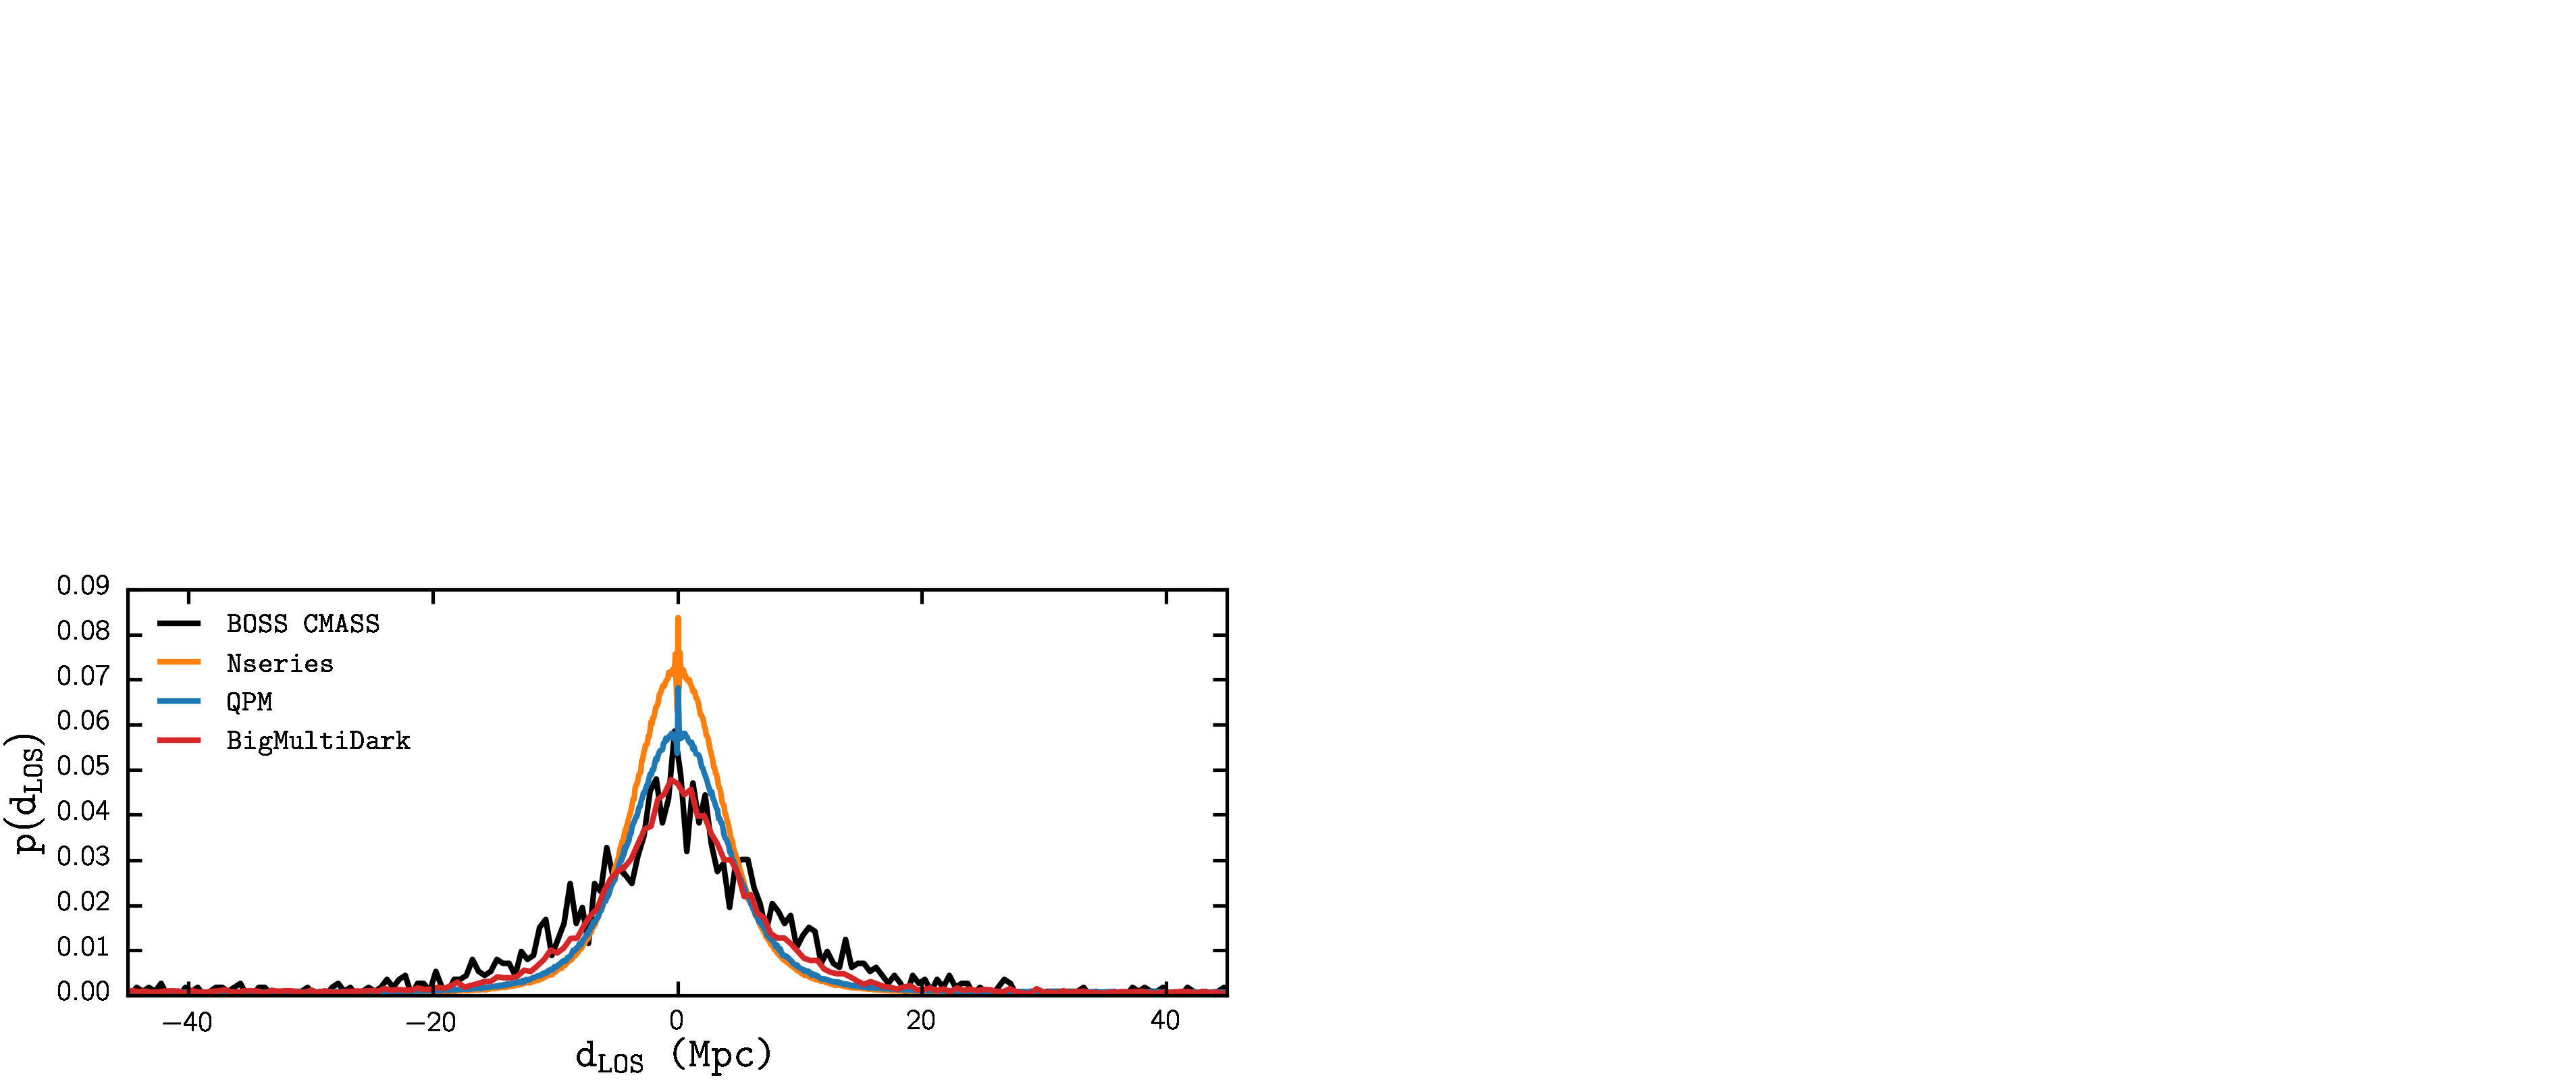
\includegraphics[width=1.\textwidth]{figs/fc/mock_catalog_dlos.pdf}
\caption{
Normalized distribution of $d_{\mathrm{LOS}}$ for Nseries
(\nseriescolor), QPM (\qpmcolor), and BigMultiDark (\tmcolor) 
mock catalogs. The normalized $d_{\mathrm{LOS}}$ distribution of 
BOSS DR12 is also plotted (\cmasscolor). The mock catalog distributions 
have bin sizes of $\Delta d = 0.2\, \mathrm{Mpc}$, while the CMASS distribution has
a bin size of $\Delta d = 0.5\, \mathrm{Mpc}$. The distribution extends beyond 
the range of the above plot to $\sim \pm 500 \; \mathrm{Mpc}$. 
In the discussion of Section \ref{sec:dlospeak}, we focus mainly 
on the peak of the distribution at roughly
$-20 \; \mathrm{Mpc} < d_\mathrm{LOS} < 20 \;\mathrm{Mpc}$.} 
\label{fig:d_los}
\end{center}
\end{figure*}
%%%%%%%%%%%%%%%%%%%%%%%%%%%%%%%%%%%%%%%%%%%%%%%%%%%%%%%%%%%%%%%%%%%%%%%%%%%%%%
% DLOSPEAK METHOD 
%%%%%%%%%%%%%%%%%%%%%%%%%%%%%%%%%%%%%%%%%%%%%%%%%%%%%%%%%%%%%%%%%%%%%%%%%%%%%%
\subsection{Line-of-Sight Reconstruction Method} \label{sec:dlospeak}
% LOS DISPLACEMENT %%%%
\subsubsection{Line-of-Sight Displacement of Fiber Collided Pairs} \label{sec:dlos}
It is impossible to determine definitively from observed galaxy data whether 
individual fiber collided galaxies without resolved spectroscopic redshifts 
are correlated or chance alignments. However, the line-of-sight displacement of 
fiber collided galaxy pairs with resolved redshifts make it possible to model 
the overall impact fiber collisions have on displacing galaxies.

For the BOSS galaxy catalog, fiber collided pairs with resolved spectroscopic 
redshifts are mainly located in the overlapping regions (Section \ref{sec:catalog}).
For the simulated mock catalogs, fiber collisions are post-processed after 
the galaxy positions are generated. Therefore, 
all galaxies in fiber collided pairs have resolved redshifts. From these resolved 
redshifts we calculate the comoving line-of-sight displacement ($d_{\mathrm{LOS}}$) 
by taking the difference between the line-of-sight comoving distance of the 
resolved redshifts: 
\begin{equation}
d_{\mathrm{LOS}} = D_{\mathrm{C}} (z_1) - D_{\mathrm{C}} (z_2). 
\end{equation}
$D_{\mathrm{C}}(z)$ here is the line-of-sight comoving distance at $z$ 
(\citealt{Hogg:1999aa}), and $z_1$ and $z_2$ represent the resolved redshifts 
of the two galaxies in the fiber collided pair.

The normalized distributions of the calculated $d_\mathrm{LOS}$ for all
resolved fiber collided pairs are presented in Figure \ref{fig:d_los}
for Nseries (\nseriescolor), QPM (\qpmcolor), BigMultiDark (\bmdcolor), and BOSS DR12 
(\cmasscolor). The $d_{\mathrm{LOS}}$ distributions for all catalogs 
consist of two components: a peak roughly within the range $-20\;\mathrm{Mpc} 
< d_{\mathrm{LOS}} < 20\;\mathrm{Mpc}$ and a flat component (hereafter ``tail" component) 
outside the peak that extends to $d_{\mathrm{LOS}} \sim \pm 500 \;\mathrm{Mpc}$. The 
entire range of the distribution is not displayed in Figure \ref{fig:d_los}. 
For BOSS, as mentioned above, the $d_\mathrm{LOS}$ distribution only reflects the 
$d_\mathrm{LOS}$ values from galaxy pairs within the fiber collision angular scale 
with resolved spectroscopic redshifts, mostly from overlapping regions of the survey.

Galaxies within the same halo, due to their gravitational interactions at halo-scales, 
are more likely to be in close angular proximity with each other. These galaxies in 
over-dense regions cause the peak in the $d_{\mathrm{LOS}}$ distribution. The ``tail" 
component consists of chance aligned galaxy pairs that happen to be in close angular 
proximity in the sky. 

Focusing on the peak of the distribution, we note that it closely traces 
a Gaussian functional form. Therefore, we fit
\begin{equation} \label{eq:peak} 
p(d_{\mathrm{LOS}}) = A \; e^{-{d_{\mathrm{LOS}}^2}/{2\sigma_\mathrm{LOS}^2}}
\end{equation}
for an analytic prescription of the $d_{\mathrm{LOS}}$ distribution peak as a 
function of $d_\mathrm{LOS}$ for each of the mock catalogs. We list the 
best-fit $\sigma_\mathrm{LOS}$ obtained by fitting Eq.~(\ref{eq:peak}) to the 
$d_{\mathrm{LOS}}$ distribution peak using 
MPFIT (\citealt{Markwardt:2009aa}) in Table \ref{tab:mpfit}. The parameter values
in Table \ref{tab:mpfit} and Figure \ref{fig:d_los} illustrate that the 
$d_{\mathrm{LOS}}$ distributions for the mock catalogs closely trace 
the BOSS DR12 distribution, which encourages our use of these mock 
catalogs in our investigation.  
%%%%%%%%%%%%%%%%%%%%%%%%%%%%%%%%%%%%%%%%%%%%%%%%%%%%%%%%%%%%%%%%%%%%%%%%%%%%%%
% DLOS Peak Best-fit Table 
%%%%%%%%%%%%%%%%%%%%%%%%%%%%%%%%%%%%%%%%%%%%%%%%%%%%%%%%%%%%%%%%%%%%%%%%%%%%%%
\begin{table} 
\caption{$d_{\mathrm{LOS}}$ Distribution Best-fit Parameters} \label{tab:mpfit}
\begin{spacing}{1.5}
\begin{center}
\leavevmode
\begin{tabular}{ccc} \hline \hline
Catalog &$\sigma_\mathrm{LOS}$ ($\mathrm{Mpc}$) & $f_{\mathrm{peak}}$\\ \hline
Nseries&3.88&0.69\\
QPM&4.35&0.62\\
BigMultiDark&5.47&0.60\\ 
CMASS&6.56&0.70\\ \hline
\end{tabular} \par
%\begin{tabular}{ccc} \hline \hline
%Catalog &$\sigma$ ($\mathrm{Mpc}$) & $f_{\mathrm{peak}}$\\ \hline
%Nseries  & 6.85  & 0.71 \\ 
%QPM        & 4.98  & 0.65 \\ 
%Big Multidark    & 5.38  & 0.57 \\ 
%\end{tabular} \par
\end{center}
\end{spacing}
%    \bigskip 
{\bf Notes}: Best-fit parameter $\sigma_\mathrm{LOS}$ (Eq.~\ref{eq:peak}) and peak fraction $f_{\mathrm{peak}}$ (Eq.~\ref{eq:fpeak}) for the $d_{\mathrm{LOS}}$ distributions in Figure \ref{fig:d_los}. 
\smallskip
\end{table}
%%%%%%%%%%%%%%%%%%%%%%%%%%%%%%%%%%%%%%%%%%%%%%%%%%%%%%%%%%%%%%%%%%%%%%%%%%%%%%
%%%%%%%%%%%%%%%%%%%%%%%%%%%%%%%%%%%%%%%%%%%%%%%%%%%%%%%%%%%%%%%%%%%%%%%%%%%%%%

Using the best-fit to the peak of the $d_{\mathrm{LOS}}$ distribution, 
we estimate the fraction of collided pairs that are within the peak as 
the ratio of pairs with $|d_\mathrm{LOS}| < 3\sigma_\mathrm{LOS}$ 
over the total number of pairs:  
\begin{equation} \label{eq:fpeak}
f_{\mathrm{peak}} = \frac{\sum\limits_{|d_\mathrm{LOS}| < 3 \sigma_\mathrm{LOS}} p(d_{\mathrm{LOS}})}{N_{\mathrm{pairs}}}, 
\end{equation}
where $N_{\mathrm{pairs}}$ is the total number of fiber collided pairs. 
$f_\mathrm{peak}$ roughly corresponds to the fraction of galaxy pairs that are 
correlated. The $f_{\mathrm{peak}}$ values calculated for the mock catalogs are
listed in Table \ref{tab:mpfit}. They are consistent with the BOSS DR12 $f_\mathrm{peak}$. 

For the NN method of the previous section to be entirely correct, 
the $d_{\mathrm{LOS}}$ distribution in Figure \ref{fig:d_los} would 
have to be a delta function, which is clearly not the case. By simply 
incorporating the peak of the $d_{\mathrm{LOS}}$ distribution, we 
can significantly improve clustering statistics on small scales. Rather 
than placing the fiber collided galaxy on top of its nearest angular 
neighbor as the NN correction does, placing the fiber collided galaxy at a 
line-of-sight displacement, sampled from the peak of the $d_{\mathrm{LOS}}$
distribution, away from its nearest neighbor better reconstructs the 
galaxy clustering on small scales. 

%%%%%%%%%% KEY paragraph %%%%%%%% at the end we use SOME of the LOS info, not all! 
% Note that to  reconstruct the full $d_{\mathrm{LOS}}$ distribution, one would have to sample from it (obtained from overlap tiling regions) to assign redshifts of the collided galaxies. However, here is where one runs into a difficulty: on an object by object basis one does not know a priori if it is physically associated with the colliding galaxy (belonging to a peak) or a chance alignment (belonging to the tail). Therefore, undoing the delta function LOS distribution (given by the NN method) into the correct LOS distribution will make significant mistakes (in object by object basis) particularly for the  fraction $(1-f_\mathrm{peak})$ of collided galaxies that are deemed to be in the tail of the distribution. As a result, it is more accurate to displace only $f_\mathrm{peak}$ of the collided pairs, the fraction that is deemed to be correlated, while the other $(1-f_\mathrm{peak})$ pairs should retain their NN weights. Mistakes will still happen, but for pairs that are physical and are assigned NN weights, we are overestimating the small-scale power, while for chance alignment pairs that are assigned  

% one should not mistake tail objects by uncorrelated, they are approx uncorrelated to the galaxy they collide with, but they are correlated with others, so putting something random is not a good idea after all. NN uses all the positions that are already in the mix, so correlations are preserved up to weights which can be corrected.


Only $f_\mathrm{peak}$ of the 
collided pairs should be displaced, since only $f_\mathrm{peak}$ of the fiber 
collided pairs are correlated. Meanwhile, the other $(1-f_\mathrm{peak})$ pairs 
should retain their NN weights since they are uncorrelated. Displacing these galaxies as well according to the tail piece of the $d_{\mathrm{LOS}}$ distribution is not desirable because  in an object by object basis we do not know which galaxies should actually be in the tail of the distribution, thus we will be making large mistakes in $d_{\mathrm{LOS}}$ galaxy by galaxy. In addition, it is difficult to incorporate that these galaxies should be correlated with others and ignoring this modifies large-scale power. In our approach, the remaining $(1 - f_\mathrm{peak})$ fiber collided pairs are thus kept with their NN weights, and this is reflected in the shot noise correction of our estimator (Eq.~\ref{eq:roman_shotnoise}), which in turn makes connection to previous methods in the literature as we now discuss.

%%%%%%%%%%%%%%%%%%%%%%%%%%%%%%%%%%%%%%%%%%%%%%%%%%%%%%%%%%%%%%%%%%%%%%%%%%%%%%
% SHOT NOISE CORRECTION 
%%%%%%%%%%%%%%%%%%%%%%%%%%%%%%%%%%%%%%%%%%%%%%%%%%%%%%%%%%%%%%%%%%%%%%%%%%%%%%

% People dicuss shot noise correction in the context of FOurier space thinking that adjusting the shot noise is enough to correct fiber collisions, but of course this is not true. First, if this were true the 2pt function would show no correction; second, fiber collisions would only affect the power spectrum monopole. None of these things is the case. Nevertheless since this has received significant attention in the literature we discuss it in detail in this section. 

\subsubsection{Shot Noise Corrections} \label{sec:shotnoise} 
Measurements of the power spectrum are made on observations of discrete 
distributions of galaxies rather than continuous density fields. The 
discreteness contributes to the power spectrum. In order to correct for 
this contribution, galaxies are assumed to be Poisson samplings of the 
underlying distribution and a shot noise correction term 
is included in the power spectrum estimator \citep{Peebles:1980aa, Feldman:1994aa}. 

The expectation value of the shot noise term takes the following form \citep{Feldman:1994aa},
\begin{equation} \label{eq:integral_shotnoise}
P_\mathrm{shot} = \frac{ (1+\alpha) \int d^3r \;\bar{n}({\bf r})w^2({\bf r})}{\int\limits^{ } d^3r \;\bar{n}^2({\bf r})w^2({\bf r})}. 
\end{equation}

\noindent Note that for the case of uniform weights ($w={\rm const.}$), 
constant number density and no random catalog this reduces to the standard 
shot-noise Poisson correction $P_\mathrm{shot} =\bar{n}^{-1}$. 
In practice the integrals in Eq.~(\ref{eq:integral_shotnoise}) can be 
written as discrete sums over the synthetic random catalog 
\citep{Feldman:1994aa}. $\int d^3r \; \bar{n}({\bf r}) ...$ 
is computed as $\alpha \sum_{\mathrm{ran}}...$. Then the shot noise term 
becomes, 
\begin{equation} \label{eq:fkp_shotnoise}
P^\mathrm{FKP}_\mathrm{shot} = \frac{(1+\alpha) \alpha \sum\limits_{\mathrm{random}} w_\mathrm{FKP}^2({\bf r})}{\alpha \sum\limits_{\mathrm{random}}^{ } \bar{n}({\bf r})\; w_\mathrm{FKP}^2({\bf r})}.
\end{equation} 
This however, represents the expectation value of the shot noise, not the actual value 
(\citealt{Hamilton:1997aa}) since all quantities involved are mean values (calculated through the random catalog). To use the full information provided by the data, the shot noise of the galaxies should be computed from the actual galaxy weights, not the randoms. This simply corresponds to taking the self-pairs in the power spectrum estimator, Eq.~(\ref{eq:roman_p0k}), which leads to Eq.~(\ref{eq:roman_shotnoise}) and we can rewrite here as,

\beqa \label{eq:ourshot}
P^\mathrm{Hahn+}_\mathrm{shot} &=& \frac{\sum\limits_{\mathrm{galaxy}} w^2_\mathrm{FKP}({\bf r})\, w^2_\mathrm{tot}({\bf r}) + \alpha^2 \sum\limits_{\mathrm{random}} w_\mathrm{FKP}^2({\bf r})}{\alpha \sum\limits^{ }_{\mathrm{random}} \bar{n}({\bf r})\, w_\mathrm{FKP}^2({\bf r})}\nonumber  \\ & & 
\eeqa
where $\alpha = (\sum_\mathrm{gal} w_\mathrm{tot} )/N_r$. 
We emphasize that this is {\em the} shot noise of the estimator. 
In other words, if one takes the limit $k \to \infty$, the 
estimator in Eq.~(\ref{eq:roman_p0k}) will approach this 
value if no shot-noise subtraction is applied. The systematic 
effects from completeness, redshift failures and fiber collisions are accounted for through $w_\mathrm{tot}$ of the observed galaxies. In our case, $w_\mathrm{tot}=w_\mathrm{sys}$ for the resolved $f_\mathrm{peak}$ fraction of galaxies that have been displaced away from their NN positions, while $w_\mathrm{tot}>w_\mathrm{sys}$ for the $(1-f_\mathrm{peak})$ fraction of galaxies that are deemed to be in the tail of the LOS distribution and are described by NN weights of the galaxies they collided with. 


% now connect to the literature...
% people had tried to model the effects of fc's by adjusting shot noise as a way to describe the large-scale effects of fc's
% problem: is not just a constant, does nothing for quad, does nothing for xi, the true constant depends on small scale power as we shall see so it's hard to hack it this way.

Recent work in the literature of power spectrum analysis modeled the effect of fiber collisions by solely modifying the shot noise term for the NN method \citep{Beutler:2014aa, Gil-Marin:2014aa}. 
This assumes that the effect of fiber collisions beyond NN weights is to alter the large-scale effective shot noise, and therefore that only the power spectrum monopole is affected since the quadrupole is free of shot noise. 
\cite{Beutler:2014aa} supplements the NN method with a shot noise correction term given by,
\begin{equation} \label{eq:florian}
P^\mathrm{B2014}_\mathrm{shot} = \frac{\sum\limits_{\mathrm{galaxy}} w^2_\mathrm{FKP}w_\mathrm{tot}({\bf r})w_\mathrm{sys}({\bf r}) + 
\alpha^2 \sum\limits_{\mathrm{random}} w_\mathrm{FKP}^2({\bf r})}
{\alpha \sum\limits_{\mathrm{random}}^{ } \bar{n} \; w_\mathrm{FKP}^2({\bf r})}.
\end{equation}
Note that in the first term of the numerator in this equation $w_\mathrm{fc}$ is only 
included in $w_\mathrm{tot}$ as it does not enter in $w_\mathrm{sys}$. 
We note that beyond their choice of Eq.~(\ref{eq:florian}) 
for the shot noise correction term, \cite{Beutler:2014aa} marginalizes over 
a constant stochasticity term in their analysis \citep[see Eq.~40 in][]{Beutler:2014aa}.
Thus, the impact of this particular choice is not straightforward. 
%It is also worth noting that \cite{Beutler:2014aa} ends up marginalizing over the value of the shot noise in their analysis, thus the impact of this particular choice is not straightforward.


Meanwhile, \cite{Gil-Marin:2014aa} constructs $P_\mathrm{shot}$ using two separate 
components: one for ``true pairs'' and the other for ``false pairs". 
The shot-noise contribution to the power from ``true pairs'' is the same as 
Eq.~(\ref{eq:florian}) while the ``false pairs'' shot-noise contribution is 
(same as Eq.~\ref{eq:ourshot}), 
\begin{equation} \label{eq:gm_falsepairs}
P^\mathrm{False}_\mathrm{shot} = \frac{\sum\limits_{\mathrm{galaxy}} w^2_\mathrm{FKP}w^2_\mathrm{tot}({\bf r}) + 
\alpha^2 \sum\limits_{\mathrm{random}} w_\mathrm{FKP}^2({\bf r})}
{\alpha \sum\limits^{ }_{\mathrm{random}} \bar{n} \; w_\mathrm{FKP}^2({\bf r})}.
\end{equation}
\cite{Gil-Marin:2014aa} calculates the total $P_\mathrm{shot}$ as the 
weighted combination of $P^\mathrm{True}_\mathrm{shot}$ and
$P^\mathrm{False}_\mathrm{shot}$: 
\begin{equation} \label{eq:gm_shot}
P^\mathrm{GM2014}_\mathrm{shot} = (1- x_\mathrm{PS}) P^\mathrm{True}_\mathrm{shot} +
x_\mathrm{PS}\, P^\mathrm{False}_\mathrm{shot}
\end{equation}
In their analysis, \cite{Gil-Marin:2014aa} use $x_\mathrm{PS} = 0.58$, 
which they infer by measuring the difference between 
the true and the fiber-collided power spectrum monopole in the $\mathtt{PTHalos}$ 
galaxy mock catalogs (\citealt{Manera:2013aa}). Unfortunately, since the true 
power spectrum is the measurement we are trying to recover from the observations, the 
$x_\mathrm{PS}$ parameter cannot be inferred or validated from the actual 
BOSS observations. Moreover, one might worry about relying $\mathtt{PTHalos}$ or similar methods that are not based on 
high resolution N-body simulations, to extract corrections for fiber collisions that depend on small-scale power. An extension of this approach is used in recent BOSS analyses  \citep{Beutler:2016aa,Grieb:2016aa,Gil-Marin:2016aa} where Eq.~(\ref{eq:gm_shot}) is used and is supplemented with a marginalization over the shot noise value. However, as we discussed above, this has no effect in the quadrupole power spectrum, which remains the same as in the NN method.

At this point it is worth casting our ``line-of-sight reconstruction" (LRec) 
method in similar language to the methods we just discussed. We treat the 
``true pairs" (what we called peak-pairs) by displacing them according to 
the peak LOS distribution, which modifies all the power spectrum multipoles, 
and use the NN method for the ``false pairs" (pairs in the tail of the LOS 
distribution). Our shot noise correction is not adjusted, rather it is the 
true shot noise from the estimator. 
%, although note that because a fraction $f_{\rm peak}$ pairs have been resolved, the weights for all such pairs is $w_\mathrm{fc}=1$, which of course will be reflected in a lower shot noise value. 
We now discuss the implementation and performance of our  LRec fiber collision method. 


%%%%%%%%%%%%%%%%%%%%%%%%%%%%%%%%%%%%%%%%%%%%%%%%%%%%%%%%%%%%%%%%%%%%%%%%%%%%%%%%%%%%
% dLOS Peak Correction P(k) Ratio Figure 
%%%%%%%%%%%%%%%%%%%%%%%%%%%%%%%%%%%%%%%%%%%%%%%%%%%%%%%%%%%%%%%%%%%%%%%%%%%%%%%%%%%%
\begin{figure*}
\begin{center}
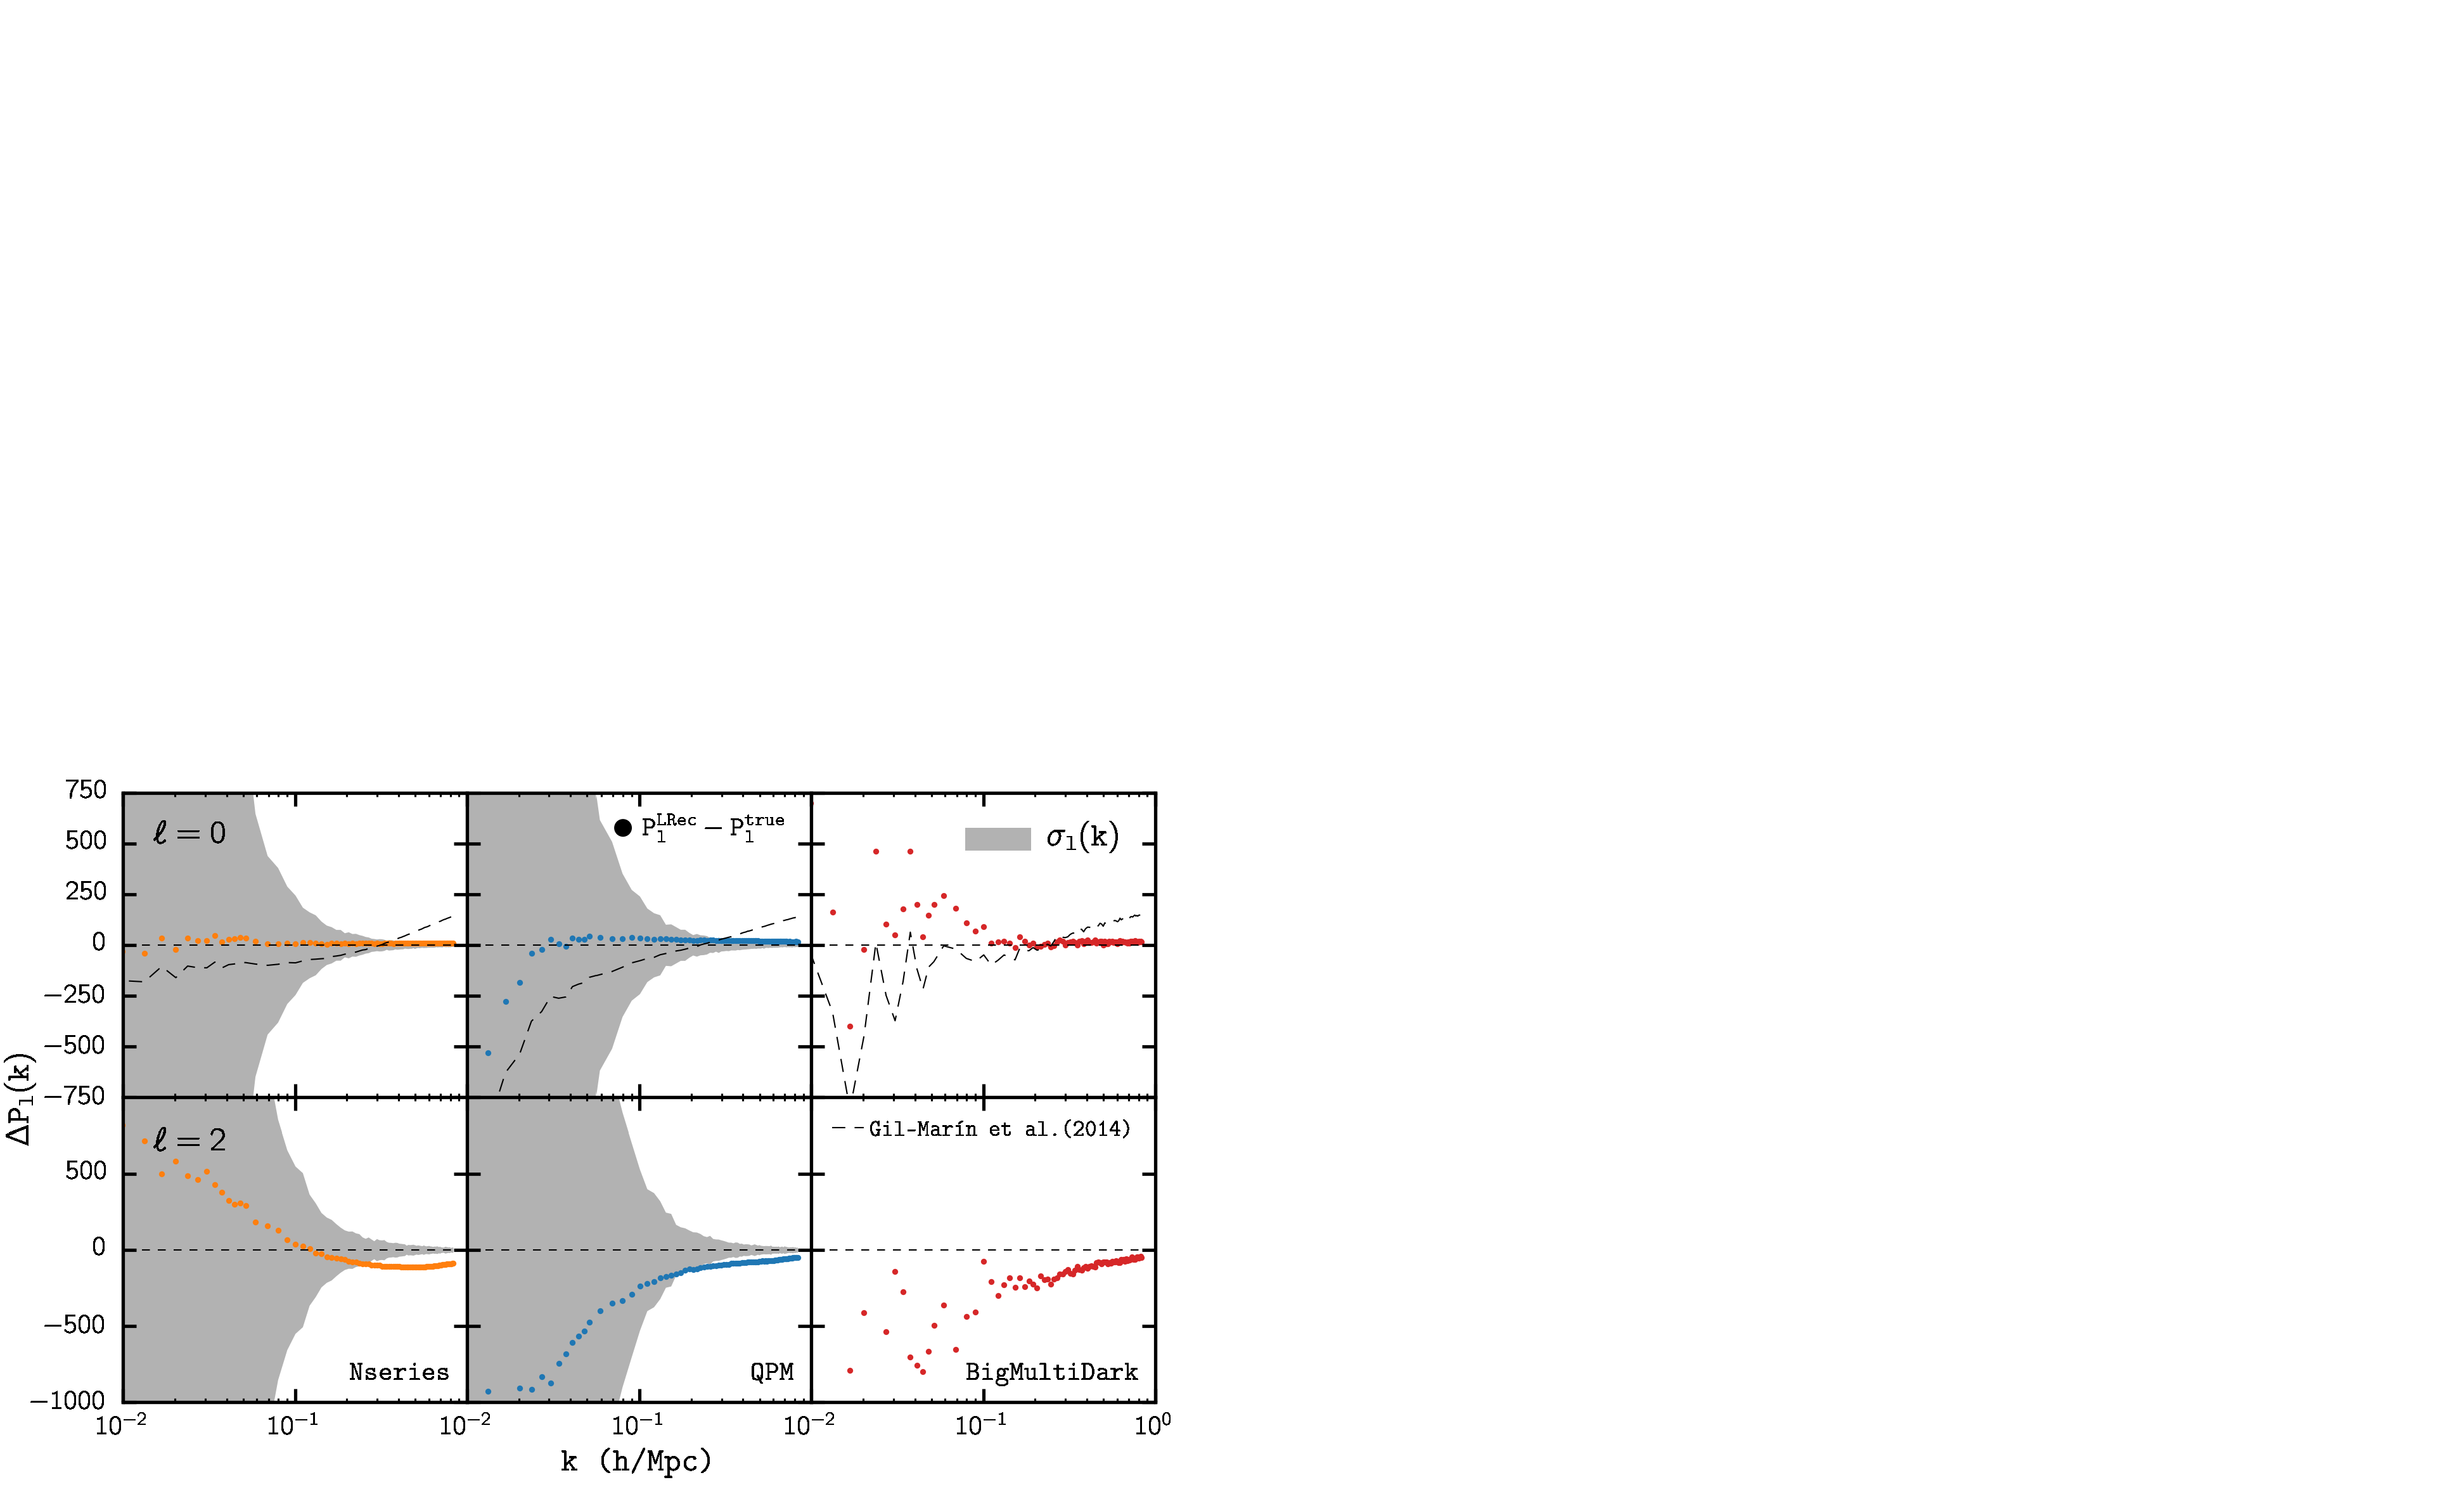
\includegraphics[width=1.\textwidth]{figs/fc/mock_catalog_dlospeak_true_Plk_resid_floran_offset250_0_rebin6x.pdf} 
\caption{The power spectrum residual of the line-of-sight reconstruction (LRec) 
method (Section \ref{sec:dlospeak}), 
$\Delta P_\ell \equiv P_l^\mathrm{LRec} -P_l^\mathrm{true}$, 
for the monopole (top) and quadrupole (bottom) power spectra of the 
Nseries (left), QPM (middle), and BigMultiDark (right) mock catalogs. 
We again plot the Nseries and QPM sample variances, $\sigma_l(k)$.
The residuals for the monopole show good agreement between 
$P_0^\mathrm{LRec}$ and $P_0^\mathrm{true}$ for the entire $k$ range. 
For the quadrupole, while the LOS Reconstruction method improves the residuals 
compared to the NN method at small scales ($k > 0.2\;h/\mathrm{Mpc}$), 
the residuals remain comparable to sample variance at $k=0.2\;h/\mathrm{Mpc}$.
In the top panels, we include the residuals from the fiber collision 
correction method of \cite{Gil-Marin:2014aa} (dashed). 
As the \cite{Gil-Marin:2014aa} method supplements 
the NN method with adjustments to the constant shot noise term of the estimator, 
it fails to correct for the $k$ dependence of the effect and is insufficient 
in accounting for fiber collisions at small scales. 
We do not include the correction method of \cite{Beutler:2014aa} because they 
marginalize over a constant stochasticity term in their analysis so the effect 
of their correction on $P(k)$ is not straightforward.}
%so we plot the correction from Eq.~(\ref{eq:florian}) offset by $-250$ to match 
%low-$k$ residuals on the left panel.}} 
\label{fig:peaksn}
\end{center}
\end{figure*}

\begin{figure}
\begin{center}
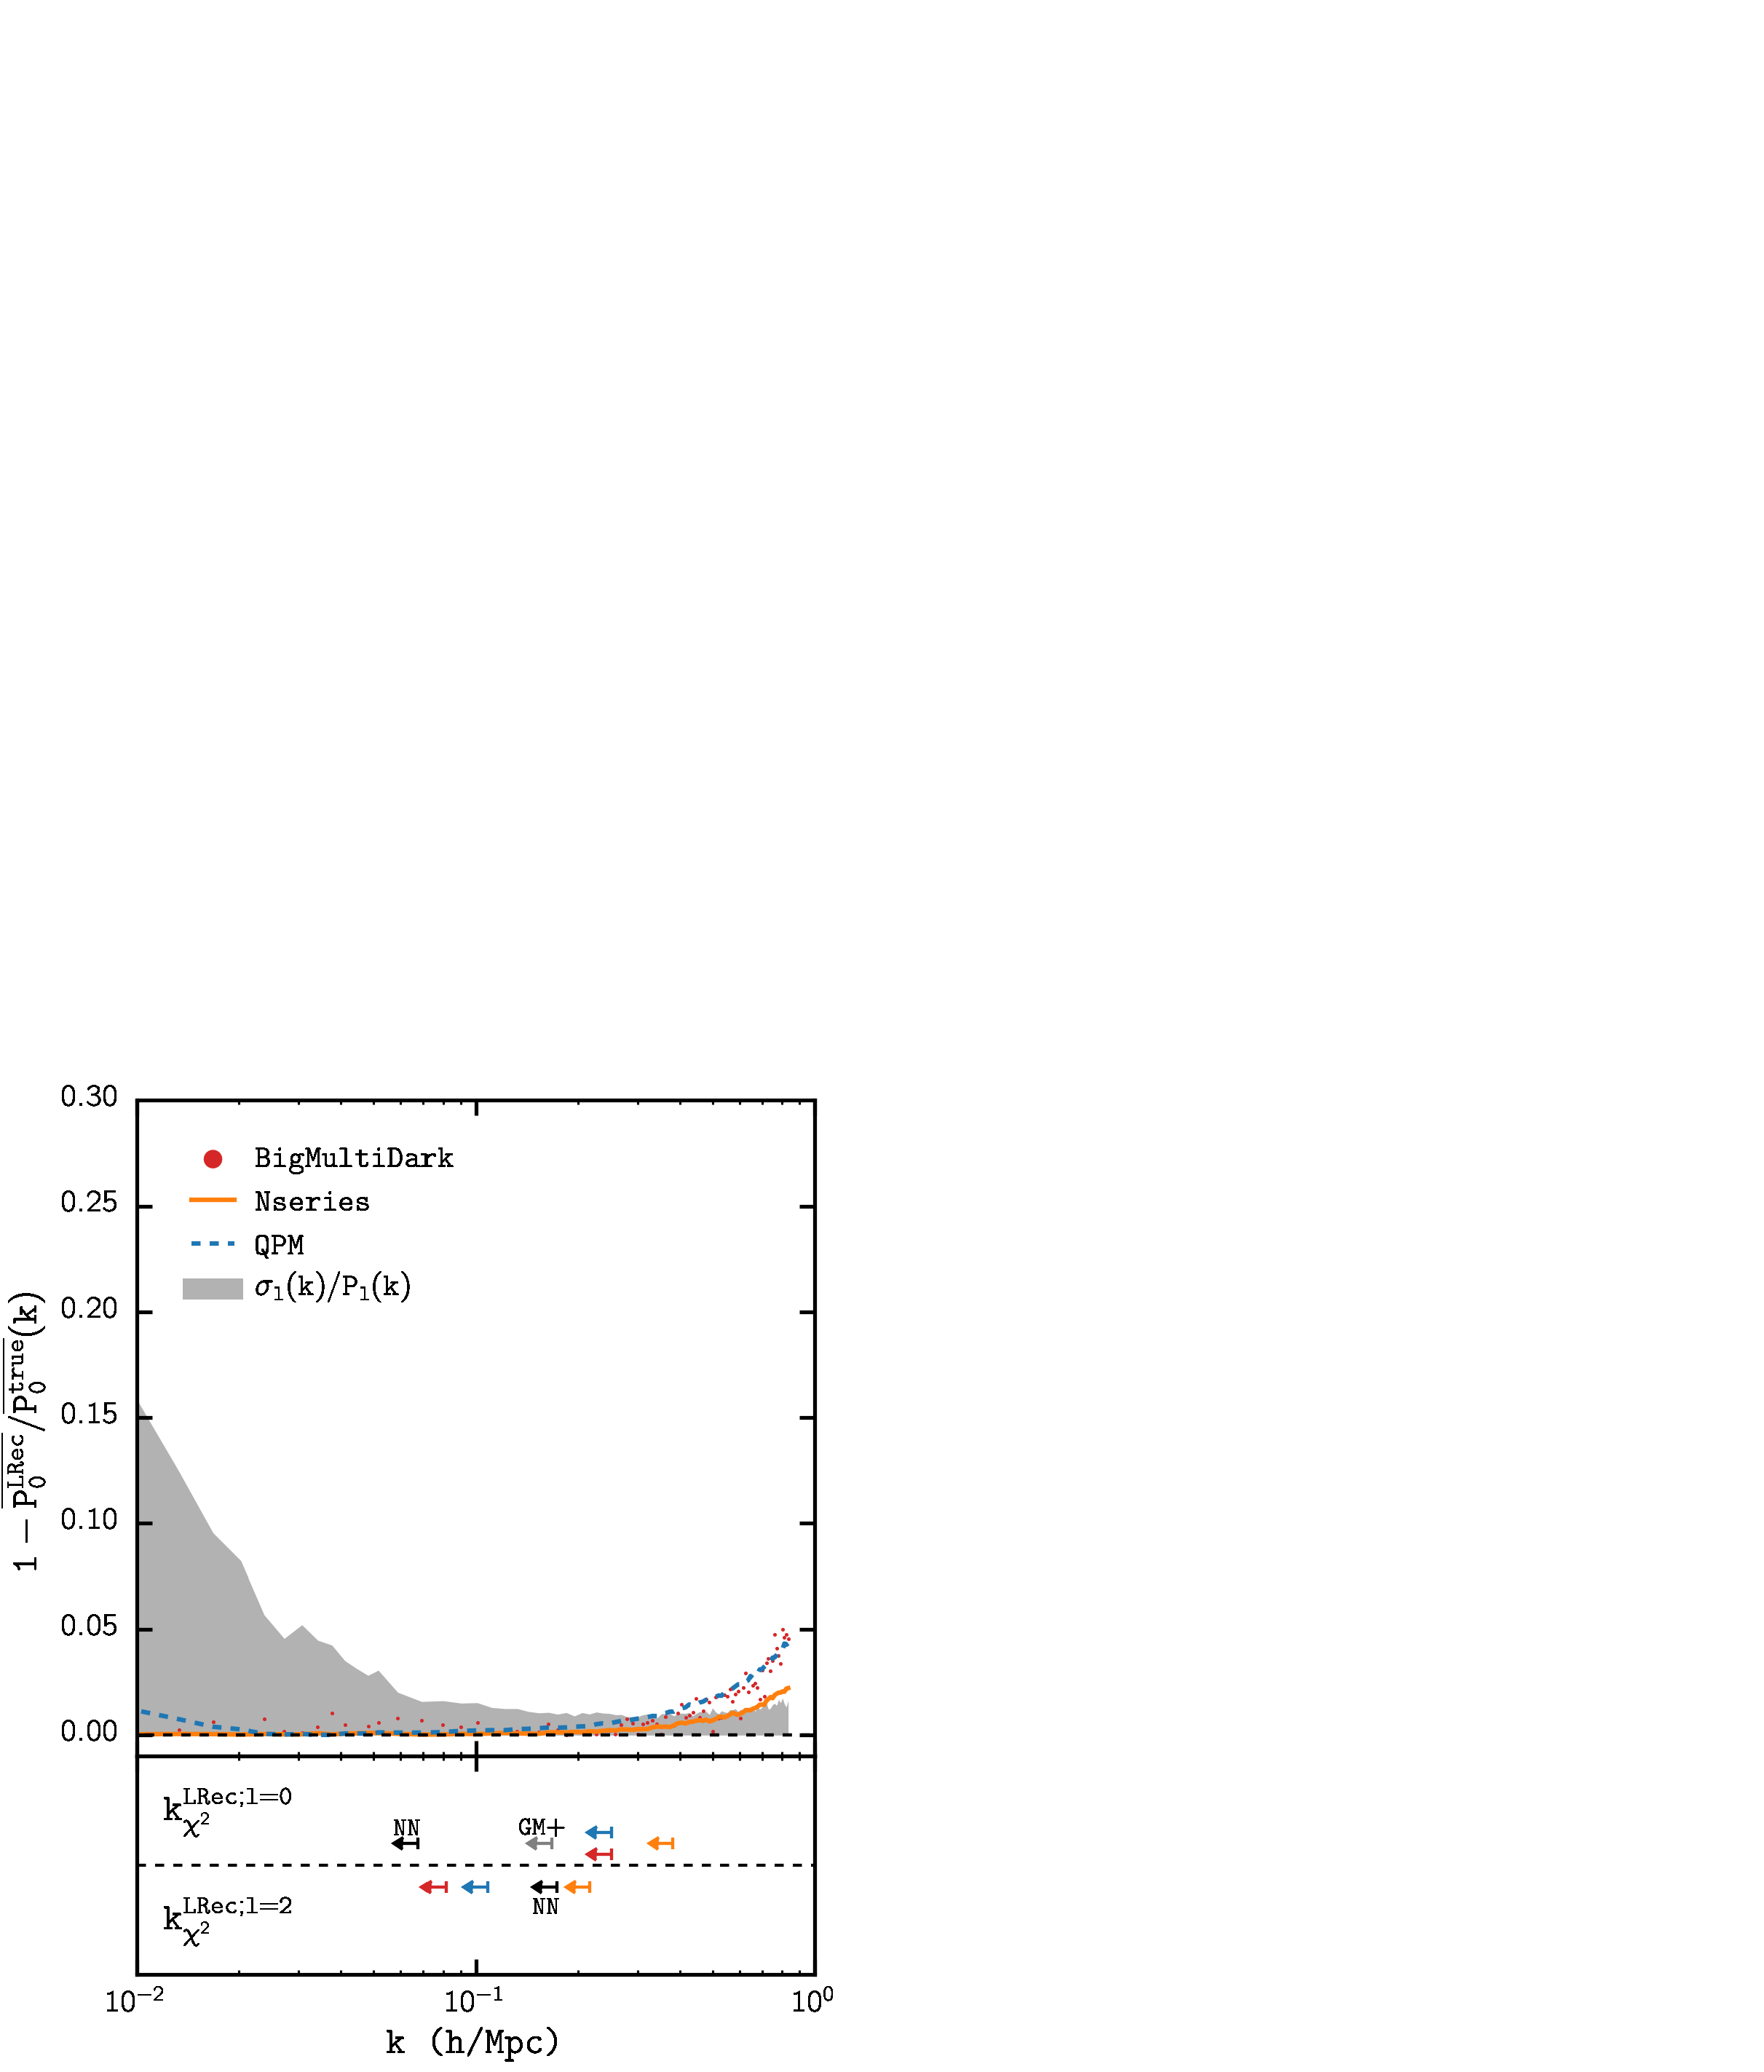
\includegraphics[width=1.\textwidth]{figs/fc/mock_catalog_dlospeak_true_P0k_norm_resid_rebin6x.pdf} 
\caption{{\it Top Panel}: The normalized residual, 
$1 - P_l^\mathrm{LRec}/P_l^\mathrm{true}$, 
for the Nseries (\nseriescolor), QPM (\qpmcolor), and BigMultiDark (\bmdcolor)
monopole power spectra. The normalized sample variance $\sigma_l / P_l(k)$ 
(gray shaded region) of the Nseries mocks is plotted for comparison. At 
$k = 0.1 \;h/\mathrm{Mpc}$, where the NN method residuals exceeds sample 
variance, the average normalized residual for the LRec method is $0.25\%$ 
compared to $1.5\%$ normalized sample variance. In fact, the average 
residual stays below the sample variance until $k = 0.53\;h/\mathrm{Mpc}$.
{\it Bottom Panel}: We mark $k^\mathrm{LRec}_{\chi^2}$ for the monopole (arrows above the 
dashed line) and quadrupole (arrows below the dashed line). 
The average $k^\mathrm{LRec}_{\chi^2}$ for the mock catalogs
are $0.29$ and $0.14\;h/\mathrm{Mpc}$ for the monopole and quadrupole respectively. 
For comparison, we mark $k^\mathrm{NN}_{\chi^2}$ (black) from Section \ref{sec:fc_pk}. 
We also include $k_{\chi^2}$ of the \cite{Gil-Marin:2014aa} correction method (gray) for 
the monopole. The LOS reconstruction method significantly 
extends $k_{\chi^2}$ beyond that of the NN method and \cite{Gil-Marin:2014aa} for $l=0$. 
However, it does not improve $k_{\chi^2}$ for the quadrupole. 
} 
\label{fig:dlospeak_norm_resid}
\end{center}
\end{figure}
%%%%%%%%%%%%%%%%%%%%%%%%%%%%%%%%%%%%%%%%%%%%%%%%%%%%%%%%%%%%%%%%%%%%%%%%%%%%%%%%%%%%
% Correction Method in Practice 
%%%%%%%%%%%%%%%%%%%%%%%%%%%%%%%%%%%%%%%%%%%%%%%%%%%%%%%%%%%%%%%%%%%%%%%%%%%%%%%%%%%%
\subsubsection{In Practice}
We first begin with fiber collided mock catalogs with the NN 
fiber collision weights that accurately simulate the effects of 
fiber collisions on the actual BOSS observations. From this catalog, we
construct the $d_\mathrm{LOS}$ distribution, as described in Section 
\ref{sec:dlos} and fit for the best-fit parameters $\sigma_\mathrm{LOS}$ 
and $f_\mathrm{peak}$ of Eq.~(\ref{eq:peak}).

We select $f_\mathrm{peak}$ of the fiber collided galaxy pairs in the catalog 
and designate them as correlated pairs that lie within the peak of the 
$d_\mathrm{LOS}$ distribution. We refer to these fiber collided pairs as 
``peak-assigned". At this point, each of these pairs, based on their NN 
weights, consist of the ``nearest-neighbor" galaxy with $w_\mathrm{fc} > 1$ 
and the ``collided" galaxy with $w_\mathrm{fc} = 0$. We discard the collided galaxy
since the redshifts of collided galaxies are not known in actual observations. 

Next for each of the nearest-neighbor galaxies in peak-assigned pairs, we 
place a new galaxy with $w_\mathrm{fc} = 1$ at a displacement $d_\mathrm{peak}$ 
away from it along the line-of-sight but at the same angular position. The $d_\mathrm{peak}$ 
value is sampled from a Gaussian with best-fit $\sigma_\mathrm{LOS}$ from 
Table \ref{tab:mpfit}. The $w_\mathrm{fc}$ of the ``nearest-neighbor" galaxy 
is then reduced by $1$. This process is repeated, in the cases of triplets 
or higher with $w_{\rm fc} > 2$, until all the nearest-neighbor galaxy in 
peak-assigned pairs have $w_\mathrm{fc}=1$. The resulting {\em total} catalog will have fewer 
galaxies with $w_\mathrm{fc} > 1$ compared to the initial fiber collided catalog.
However, the total statistical weight ($\sum_\mathrm{gal} w_\mathrm{tot}$) of 
the catalog, being equal to the total number of galaxies before the collisions
are applied, is conserved. 
%\todo{I'm confused by this explanation, at the end of the day $w_{fc}=1$ for all, right?}

Now that we have the ``LOS reconstructed" mock catalog, we measure its power 
spectrum monopole and quadrupole ($P^\mathrm{LRec}_l$). In Figure 
\ref{fig:peaksn} we present the power spectrum residual, 
$(P^\mathrm{LRec}_l-P^\mathrm{true}_l)$,  
for $l = 0$ and $2$ of the LOS Reconstruction method power spectrum averaged over all the available realizations. 
We again include the Nseries and QPM sample variance, $\sigma_l(k)$ 
(grey shaded region) for comparison.  In Figure \ref{fig:dlospeak_norm_resid}, 
we normalize both the residuals and the sample variance by $P_0^\mathrm{true}$ 
to better compare $P_0^\mathrm{LRec}$ and $P_0^\mathrm{true}$ at different scales 
and to highlight the small scales. 

For the monopole, at the scale where $P^\mathrm{NN}_0$ deviates from 
$P^\mathrm{true}_0$ by more than the sample variance ($k \sim 0.1\;h/\mathrm{Mpc}$), 
Figure \ref{fig:peaksn} shows that the LOS reconstructed residual is well within the 
sample variance, $P^\mathrm{LRec}_0 - P^\mathrm{true}_0 < 0.17\, \sigma_0$. 
Even at the smallest scales measured for our monopole measurements 
($k = 0.83\;h/\mathrm{Mpc}$), well beyond the scales that can be predicted from current models based on perturbation theory, the normalized residuals for 
the LOS reconstructed method remains at $3.7\%$. At $k \sim 0.2\;h/\mathrm{Mpc}$, the average normalized 
residual is $0.19\%$ compared to the $0.9\%$ normalized sample variance. 
When we calculate the $k_{\chi^2}$ of the LOS reconstruction method for 
the three mock catalogs, as we did for the NN method in Section \ref{sec:fc_pk}, 
we get the average $k_{\chi^2}^\mathrm{LRec} = 0.29\;h/\mathrm{Mpc}$ for the monopole. 
For each of the mocks, we mark $k_{\chi^2}^{\mathrm{LRec};\;l=0}$ in the lower panel 
of Figure \ref{fig:dlospeak_norm_resid} above the dashed horizontal line. 


For the monopole, we also include residuals from the 
fiber collision correction method of \cite{Gil-Marin:2014aa} (dashed) in 
Figure~\ref{fig:peaksn}.
\cite{Gil-Marin:2014aa} corrects for fiber collisions by adjusting the 
constant shot noise term in the estimator in addition to the NN method 
(Section \ref{sec:shotnoise}).
However, as the NN method power spectrum residuals reveal in 
Figure \ref{fig:fc_pk}, the effect is $k$ dependent, especially 
at $k > 0.1 \;h/\mathrm{Mpc}$. 
So while this correction can reduce the residuals 
to within sample variance on large scales, it fails to account for 
the $k$ dependence, which quickly goes on to dominate sample variance 
at smaller scales, $k > 0.1 \;h/\mathrm{Mpc}$.

We also calculate $k_{\chi^2}$ for the \cite{Gil-Marin:2014aa} 
correction method using the mock catalogs, 
$k_{\chi^2}^\mathrm{GM+} = 0.17 \;h/\mathrm{Mpc}$ (gray arrow; Figure \ref{fig:dlospeak_norm_resid}), 
which is significantly lower than that of the LOS Reconstruction method. 
The LOS reconstruction method better accounts for fiber collisions at all 
scales. Furthermore, as already discussed, the \cite{Gil-Marin:2014aa} 
method does {\em not} provide corrections for the power spectrum 
quadrupole or higher multipoles, thus Figure~\ref{fig:fc_pk} still applies for $\ell=2$.

We note that the correction method of \cite{Beutler:2014aa} 
is not included in Figure~\ref{fig:peaksn}. Instead of using 
a fixed value for the constant shot noise as \cite{Gil-Marin:2014aa} does, 
\cite{Beutler:2014aa} includes a constant `stochasticity term', $N$, 
in their analysis (see Eq. 40 of \citealt{Beutler:2014aa}). This $N$ is 
within the exponential factor that models the Finger-of-God effect, so their 
correction is $k$ dependent and impacts the multipoles beyond the monopole.
However because \cite{Beutler:2014aa} marginalizes over $N$, the effect 
of this correction is not straightforward. When we use the best-fit parameter 
values from \cite{Beutler:2014aa}, we find that the correction actually 
{\em increases} the effect of fiber collisions on both the monopole 
and quadrupole. This however, neglects the impact of stochastic bias 
in the $P(k)$ model. Nevertheless, we also find that no value of $N$ in the 
\cite{Beutler:2014aa} correction can simultaneously 
account for the effect of fiber collisions in both the monopole and quadrupole.

%For the monopole, we also include the residuals from the 
%fiber collision correction methods of \cite{Beutler:2014aa} (pluses) and 
%\cite{Gil-Marin:2014aa} (dashed) in Figure \ref{fig:peaksn}. 
%Both these analyses correct for fiber collisions by adjusting the constant 
%shot noise term in the estimator in addition to the NN method (Section \ref{sec:shotnoise}).
%However, as the NN method power spectrum residuals reveal in Figure \ref{fig:fc_pk},
%the effect has a $k$ dependence, especially at $k > 0.1 \;h/\mathrm{Mpc}$.  
%So while these corrections can reduce the residuals to within sample variance 
%at large scales, they fail to account for the $k$ dependence, 
%which quickly goes on to dominate sample variance at smaller scales, 
%$k > 0.1 \;h/\mathrm{Mpc}$.  

%We note that instead of using a fixed value for the constant shot noise
%as \cite{Gil-Marin:2014aa} does, \cite{Beutler:2014aa} marginalize over 
%the constant term in their analysis. To  reflect this,
%we offset the power spectrum residual we get using Eq.~(\ref{eq:florian}) 
%by $-250$ in Figure \ref{fig:peaksn} to force agreement at $k\to 0$ 
%in the Nseries case. For simplicity, we only calculate $k_{\chi^2}$ 
%for the \cite{Gil-Marin:2014aa} correction method using the mock catalogs: 
%$k_{\chi^2}^\mathrm{GM+} = 0.17 \;h/\mathrm{Mpc}$ (gray arrow; Figure \ref{fig:dlospeak_norm_resid}), 
%which is significantly lower than that of the LOS Reconstruction method. 
%Compared to either method, the LOS reconstruction 
%method better accounts for fiber collisions at all scales. 
%{\color{red} \bf Furthermore, as already discussed, 
%the \cite{Gil-Marin:2014aa} method does not provide corrections for the power 
%spectrum quadrupole or higher multipoles, thus Figure~\ref{fig:fc_pk} 
%still applies for $\ell=2$.}

From Figure~\ref{fig:peaksn} we see that for the quadrupole, the LOS reconstruction method does not 
sufficiently improve corrections for fiber collisions compared to the NN method.
The residuals for $k > 0.2\;h/\mathrm{Mpc}$ are improved compared to Figure~\ref{fig:fc_pk}; however, they 
still exceed the sample variance. Unfortunately, these improvements on small scales
come at the cost of increased residuals on large scales. In the $k_{\chi^2}$ marked 
in Figure \ref{fig:dlospeak_norm_resid} (below the dashed line), we see that the
increased residuals at large scales actually make the average $k_{\chi^2}^\mathrm{NN} > 
k_{\chi^2}^\mathrm{LRec} = 0.14\;h/\mathrm{Mpc}$ for the quadrupole, although there is significant dispersion between the different simulations with Nseries showing improvements when compared to the NN method while the other two showing worse performance. Consequently, neither the LOS reconstruction method nor the NN method sufficiently 
account for fiber collisions in the power spectrum quadrupole. 

The shortcomings of the LOS reconstruction method for the quadrupole compared 
to the monopole does not come as a surprise since the quadrupole is more 
sensitive to getting the correct LOS displacements galaxy by galaxy 
(not just statistically), as these modify the fingers-of-god effect. 
In order to make further progress with this method one would have to 
determine for each galaxy the most likely halo in which it lives 
(this could be nearby or a distant, chance alignment), determine its 
velocity dispersion and then assign a LOS displacement consistent 
with the dispersion and the observed LOS distribution. 

Let us now discuss a few attempts that we have implemented along these lines. 
The first is incorporating more information about the fiber collided pairs 
in order to better classify 
correlated and chance alignment pairs. For example, information about 
larger scale galaxy environment in the form of the $N^{th}$ nearest neighbor 
distance ($d_{nNN}$), can be included to parameterize the $\sigma_\mathrm{LOS}$ 
and $f_\mathrm{peak}$ (Table \ref{tab:mpfit}) as a function of $d_{nNN}$. 
The $d_{nNN}$ in this case is the distance of the $n^{th}$ nearest 
neighbor of the nearest-neighbor galaxy within the fiber collided pair.  
Another way the LOS reconstructed method can be improved is by utilizing 
the photometric redshifts of the collided galaxies to improve the 
correlated/change alignment pair classification. 

We explored the LOS reconstructed method with both of these improvements 
on the mock catalogs. We find that there is indeed a significant correlation 
between $d_{nNN}$ and the parameters $\sigma_\mathrm{LOS}$ and 
$f_\mathrm{peak}$, which can be exploited. Also, photometric redshifts assigned 
to collided galaxies based on the 
$|z_\mathrm{spec} - z_\mathrm{photo}|/(1 + z_\mathrm{spec})$
of actual BOSS photometric redshift catalogs improves classification of 
correlated versus chance alignment fiber collided pairs, as well. These 
improvements bring the normalized residuals of the monopole to $\sim 1\%$
at $k = 0.83\;h/\mathrm{Mpc}$. However, the improvement in the fiber collision 
correction for the quadrupole is marginal; the effect of fiber collisions 
at $k = 0.2\;h/\mathrm{Mpc}$ is still comparable to the sample variance. So 
even with these improvements the LOS reconstructed method is insufficient. 

Furthermore, for the Nseries mocks, we find that if we use the LOS reconstructed method with 
perfectly classified correlated and chance alignment pairs, the 
residual is roughly half the sample variance at $k \sim 0.2\;h/\mathrm{Mpc}$
and greater than sample variance at $k > 0.35\;h/\mathrm{Mpc}$.
The displacement of the collided galaxy by $d_\mathrm{LOS}$ sampled from Eq.~(\ref{eq:peak}) 
alone causes the power spectrum quadrupole to deviate from the true value
at small scales. A method such as the LOS reconstructed method for the quadrupole 
would require more sophisticated modeling of the fiber collided galaxy pairs that capture the displacements in an object by object basis. 

As a result of the shortcomings of the LOS reconstructed method for the power spectrum 
quadrupole, we now present a complementary approach in dealing with fiber collision 
in power spectrum multipole analyses, which rather than attempting to correct the 
data before making measurements, computes theoretical predictions of the fiber-collided 
power spectrum multipoles. 

%%%%%%%%%%%%%%%%%%%%%%%%%%%%%%%%%%%%%%%%%%%%%%%%%%%%%%%%%%%%%%%%%%%%%%%%%%%%%%%%
% 2PCF Ratio, tophat figure
%%%%%%%%%%%%%%%%%%%%%%%%%%%%%%%%%%%%%%%%%%%%%%%%%%%%%%%%%%%%%%%%%%%%%%%%%%%%%%%%
\begin{figure*}
\begin{center}
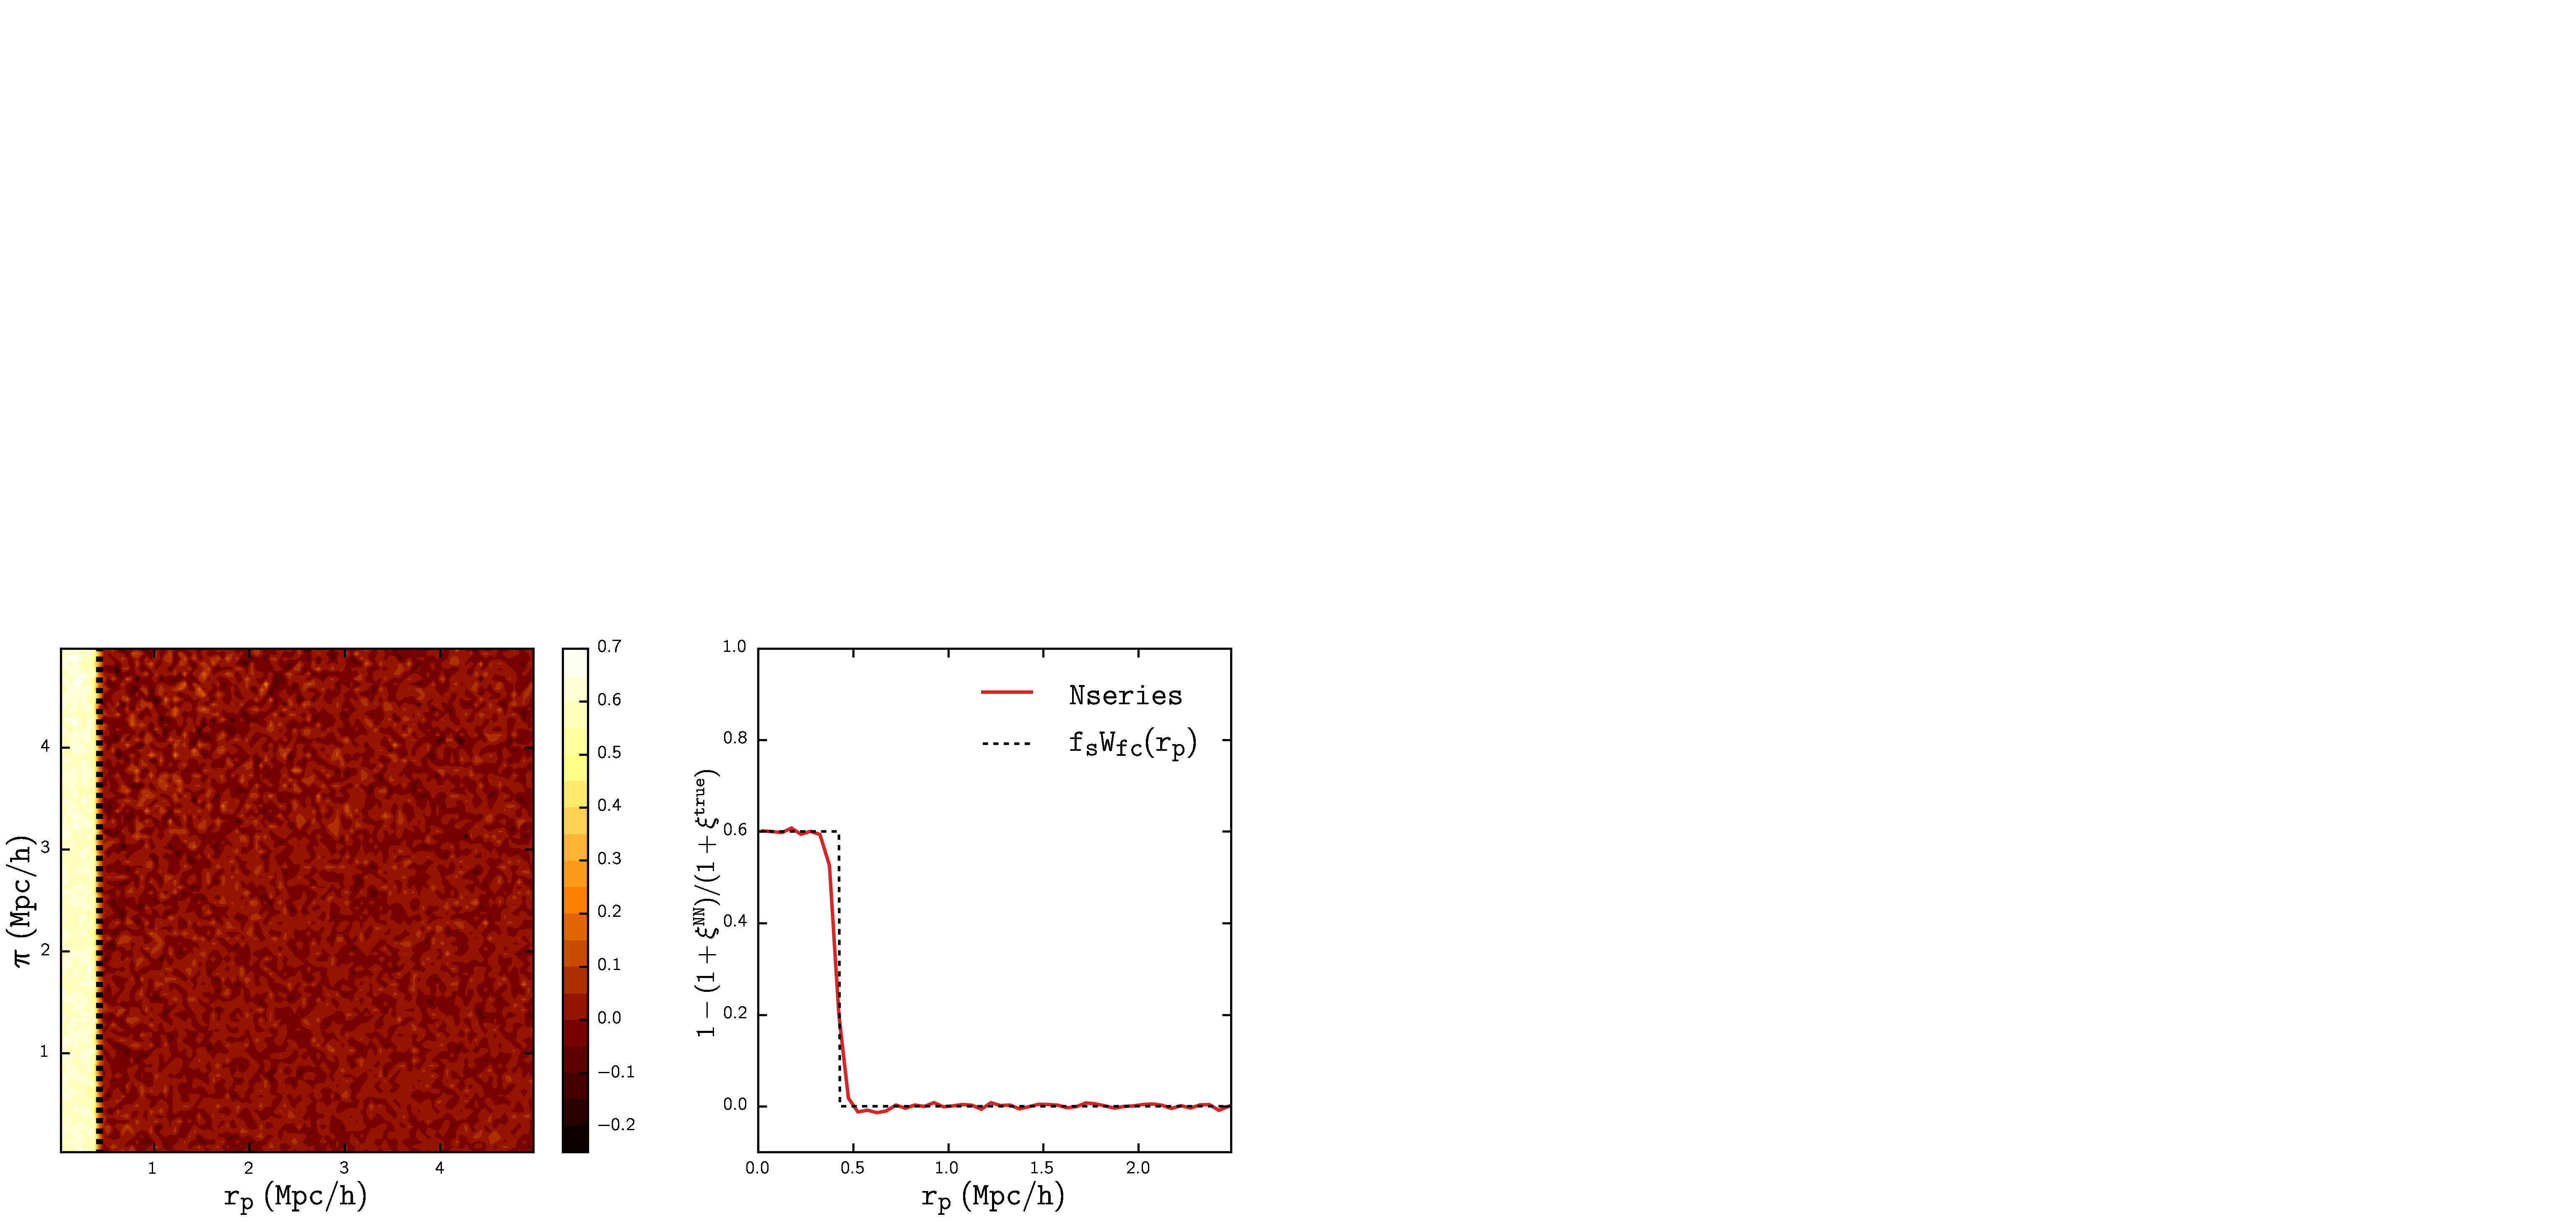
\includegraphics[width=1.\textwidth]{figs/fc/2pcf_Nseries_upweighted_5mocks_5x5_tophat.pdf} 
\caption{$1 - (1 + \xi^\mathrm{NN})/(1+\xi^\mathrm{true})$ as a 
function of transverse displacement, $r_p$, and line-of-sight 
displacement $\pi$ (left). The color bar represents the value of this quantity. Note there is no detectable dependence on $\pi$.
The dashed vertical line (black) represents the constant 
$r_p = D_\mathrm{fc}(z=0.55)$ (Section \ref{sec:fourier}). 
We also plot $1 - (1 + \xi^\mathrm{NN})/(1+\xi^\mathrm{true})$
projected along $\pi$ (right). In the left panel, the $r_p = D_\mathrm{fc}(z=0.55)$ 
vertical line and the sharp cut-off of the contour show good agreement with the expected characteristic scale. 
In the right panel, the projected $1 - (1 + \xi^\mathrm{NN})/(1+\xi^\mathrm{true})$
is in good agreement with $f_s W_\mathrm{fc}(r_p)$. The agreement in both panels
justify the characterization of the effect of fiber collisions on the 2PCF in 
Eq.~(\ref{eq:tophat_2pcf}).}
\label{fig:2pcf_tophat}
\end{center}
\end{figure*}
%%%%%%%%%%%%%%%%%%%%%%%%%%%%%%%%%%%%%%%%%%%%%%%%%%%%%%%%%%%%%%%%%%%%%%%%%%%%%%%%
% Fourier Tophat Method 
%%%%%%%%%%%%%%%%%%%%%%%%%%%%%%%%%%%%%%%%%%%%%%%%%%%%%%%%%%%%%%%%%%%%%%%%%%%%%%%%
\subsection{Effective Window Method} \label{sec:fourier}
The LOS Reconstruction method corrects for fiber collisions in the observed galaxy positions 
in order to estimate the systematics-free true power 
spectrum. In power spectrum analyses, this true power spectrum estimate
can be compared to model power spectrum for cosmological parameter inference. 
Alternatively, however, the observed fiber collided power spectrum can be 
compared to the model power spectrum with the effect of fiber collisions imposed 
on it. This is the approach we follow from now on.

We proceed as follows. In Section \ref{sec:tophat_theory} we find that the effect of fiber collisions 
on the two-point correlation function can be well approximated by a simple 
analytic expression. Using this, we accurately estimate the 
effect of fiber collisions on the power spectrum in Fourier space. The effect 
is a function of the true power spectrum and depends significantly on the 
power spectrum at small scales, which cannot reliably be modeled from first principles. As a result, in Section~\ref{sec:tophat_practice}, we 
present a practical approach to circumvent this issue and account for the effect of fiber collisions in 
power spectrum analyses. 

\subsubsection{In Theory} \label{sec:tophat_theory}
In the BOSS galaxy catalog, which spans the redshifts $0.43 < z < 0.7$, 
the comoving distance of the $62"$ fiber collision angular scale 
($D_\mathrm{fc}$) ranges from $0.35\;\mathrm{Mpc}$ to $0.52\;\mathrm{Mpc}$. 
Given the relatively small variation in $D_\mathrm{fc}$, we assume 
that throughout the survey redshift the physical scale remains
constant as $D_\mathrm{fc}(z \sim 0.55) = 0.43 \mathrm{Mpc}$, at the median 
redshift of the survey. If the physical scale of fiber collisions is constant, 
fiber collisions will affect the two-dimensional configuration space two-point 
correlation function, $\xi(r_p, \pi)$, through its effect on galaxy pairs with 
transverse separations $r_p < D_\mathrm{fc}$. As no pairs will be found 
below this characteristic scale, $\xi(r_p, \pi)$ will be -1 
for $r_p < D_\mathrm{fc}$, and note that  the same is true for the two-point function in the NN method (since small-$r_p$ pairs are collapsed into zero separation described by weights). On the other hand, at large scales we can approximate $\xi(r_p, \pi)$ by the NN method which preserves the large-scale angular correlation function, thus 
the effect of fiber collisions on $\xi(r_p, \pi)$ can be analytically characterized by  the following relation between the true and the NN two-point functions,
\begin{equation} \label{eq:tophat_2pcf}
\frac{1 + \xi^\mathrm{NN}(r_p, \pi)}{1 + \xi^\mathrm{true}(r_p, \pi)} =1 -  f_s W_\mathrm{fc}(r_p)
\end{equation}
where $W_\mathrm{fc}(r_p)$ represents the top-hat function
\begin{spacing}{1.5}
\begin{equation} \label{eq:tophat}
W_\mathrm{fc}(r_p) = 
\begin{cases}
1 & \text{if}\ r_p < D_\mathrm{fc} \\
0 & \text{otherwise}
\end{cases}
\end{equation}
\end{spacing}
\noindent and $f_s$ represents the fraction of the survey area affected by fiber 
collisions. Note in Eq.~(\ref{eq:tophat_2pcf}) we have assumed that we can linearly superpose the contributions to the two-point function from regions with and without collisions, and a key property of Eq.~(\ref{eq:tophat_2pcf}) is that its right hand side does not depend on $\pi$, something we test explicitly below. 
In the BOSS, $f_s$ is precisely known because 
it corresponds to the fraction of the survey geometry that suffers from 
fiber collisions. These are the regions that do not have overlapped tiling 
(Section \ref{sec:catalog}). For BOSS DR12 $f_s = 0.6$. 

We measure $\xi^\mathrm{NN}$ and $\xi^\mathrm{true}$ for the Nseries 
mock catalogs using the $\mathtt{CUTE}$ software (\citealt{Alonso:2012aa}), which 
uses the standard \cite{Landy:1993aa} estimator. $\xi^\mathrm{NN}$ 
is calculated from the NN fiber collided Nseries mocks while 
$\xi^\mathrm{true}$ is calculated from the Nseries mocks without fiber 
collisions. Using the measured $\xi^\mathrm{NN}$ and $\xi^\mathrm{true}$, 
we plot 
$1- (1+\xi^\mathrm{NN})/(1 + \xi^\mathrm{true})$ averaged over realizations as 
a function of $r_p$ and $\pi$ (left) and its projection 
along $\pi$ (right) in Figure \ref{fig:2pcf_tophat}. The dashed vertical 
line (black; left) marking $r_p = D_\mathrm{fs}(z=0.55)$ and $f_s W_\mathrm{fc}(r_p)$ 
(black dashed; right) are plotted for comparison. The agreement 
between the $\xi(r_p, \pi)$ contours and the $r_p = D_\mathrm{fc}(z=0.55)$ 
cutoff along with the agreement between the projection and 
$f_s W_\mathrm{fc}(r_p)$ justify our assumption of a constant physical 
fiber collision scale. The exact survey tiling of the BOSS sample is 
imposed on the Nseries mocks, so we expect Figure \ref{fig:2pcf_tophat} 
to hold for the BOSS observations. The left panel illustrates 
the $\pi$-independence of the left hand side of Eq.~(\ref{eq:tophat_2pcf}). 
The right panel demonstrates that 
$1- (1+{\xi^\mathrm{NN}})/(1 + {\xi^\mathrm{true}})$ projected
along $\pi$ agrees remarkably well with a top-hat function. 

In principle, however,
$W_\mathrm{fc}$ is not necessarily a top-hat function. In fact,
in eBOSS, due to the complex targeting scheme involving ``knock-outs'' from 
higher priority targeting samples, $W_\mathrm{fc}$ will not be top-hat function 
(Zhai et al. in prep). However, these complications are not present in our implementation of collisions; the reason for the deviations from a top-hat function here can be thought as arising from a sum of top-hats of slightly different radii along the line of sight (for fixed angular scale) weighted by the probability of collisions at each depth, leading to a smoother transition than a sharp top-hat function. In principle, our formalism  can be improved by including this numerical profile rather than a top-hat, as we shall mention below (see discussion after Eq.~\ref{DeltaPell2}). 


With the confirmation of Eq.~(\ref{eq:tophat_2pcf}), we solve for $\xi^\mathrm{NN}$   
:
\beqa
\xi^\mathrm{NN}(r_p, \pi) &=& \xi^\mathrm{true}(r_p, \pi) - f_s W_\mathrm{fc}(r_p)\ (1 + \xi^\mathrm{true}(r_p, \pi)),
\nonumber \\ & & 
\eeqa

and to get an expression for the power spectrum, we Fourier transform to get 
\beqa 
\label{eq:tophat_pk}
\Delta P({\bf k}) &\equiv& P^\mathrm{NN}({\bf k}) - P^\mathrm{true}({\bf k})  \nonumber \\ & & 
= - f_s\, {W_\mathrm{fc}}({\bf k})- f_s \int {\mathrm{d}^3q\over (2\pi)^3} P({\bf q})\, {W_\mathrm{fc}}({\bf k} - {\bf q}). \nonumber \\ & & 
\eeqa
We see that the effect of fiber collisions on the true power spectrum 
can be characterized by two terms: Fourier transform of the 
top-hat function (corresponding to chance collisions) 
and the power spectrum convolved with the top-hat function (corresponding to 
physically correlated pairs). We refer to these two terms as $\Delta P^\mathrm{uncorr}$ and 
$\Delta P^\mathrm{corr}$ respectively. Note that none of these terms is independent of $k$.

%%%%%%%%%%%%%%%%%%%%%%%%%%%%%%%%%%%%%%%%%%%%%%%%%%%%%%%%%%%%%%%%%%%%%%%%%%%%%%%%
% Del P comparison figure  
%%%%%%%%%%%%%%%%%%%%%%%%%%%%%%%%%%%%%%%%%%%%%%%%%%%%%%%%%%%%%%%%%%%%%%%%%%%%%%%%
\begin{figure*}
\begin{center}
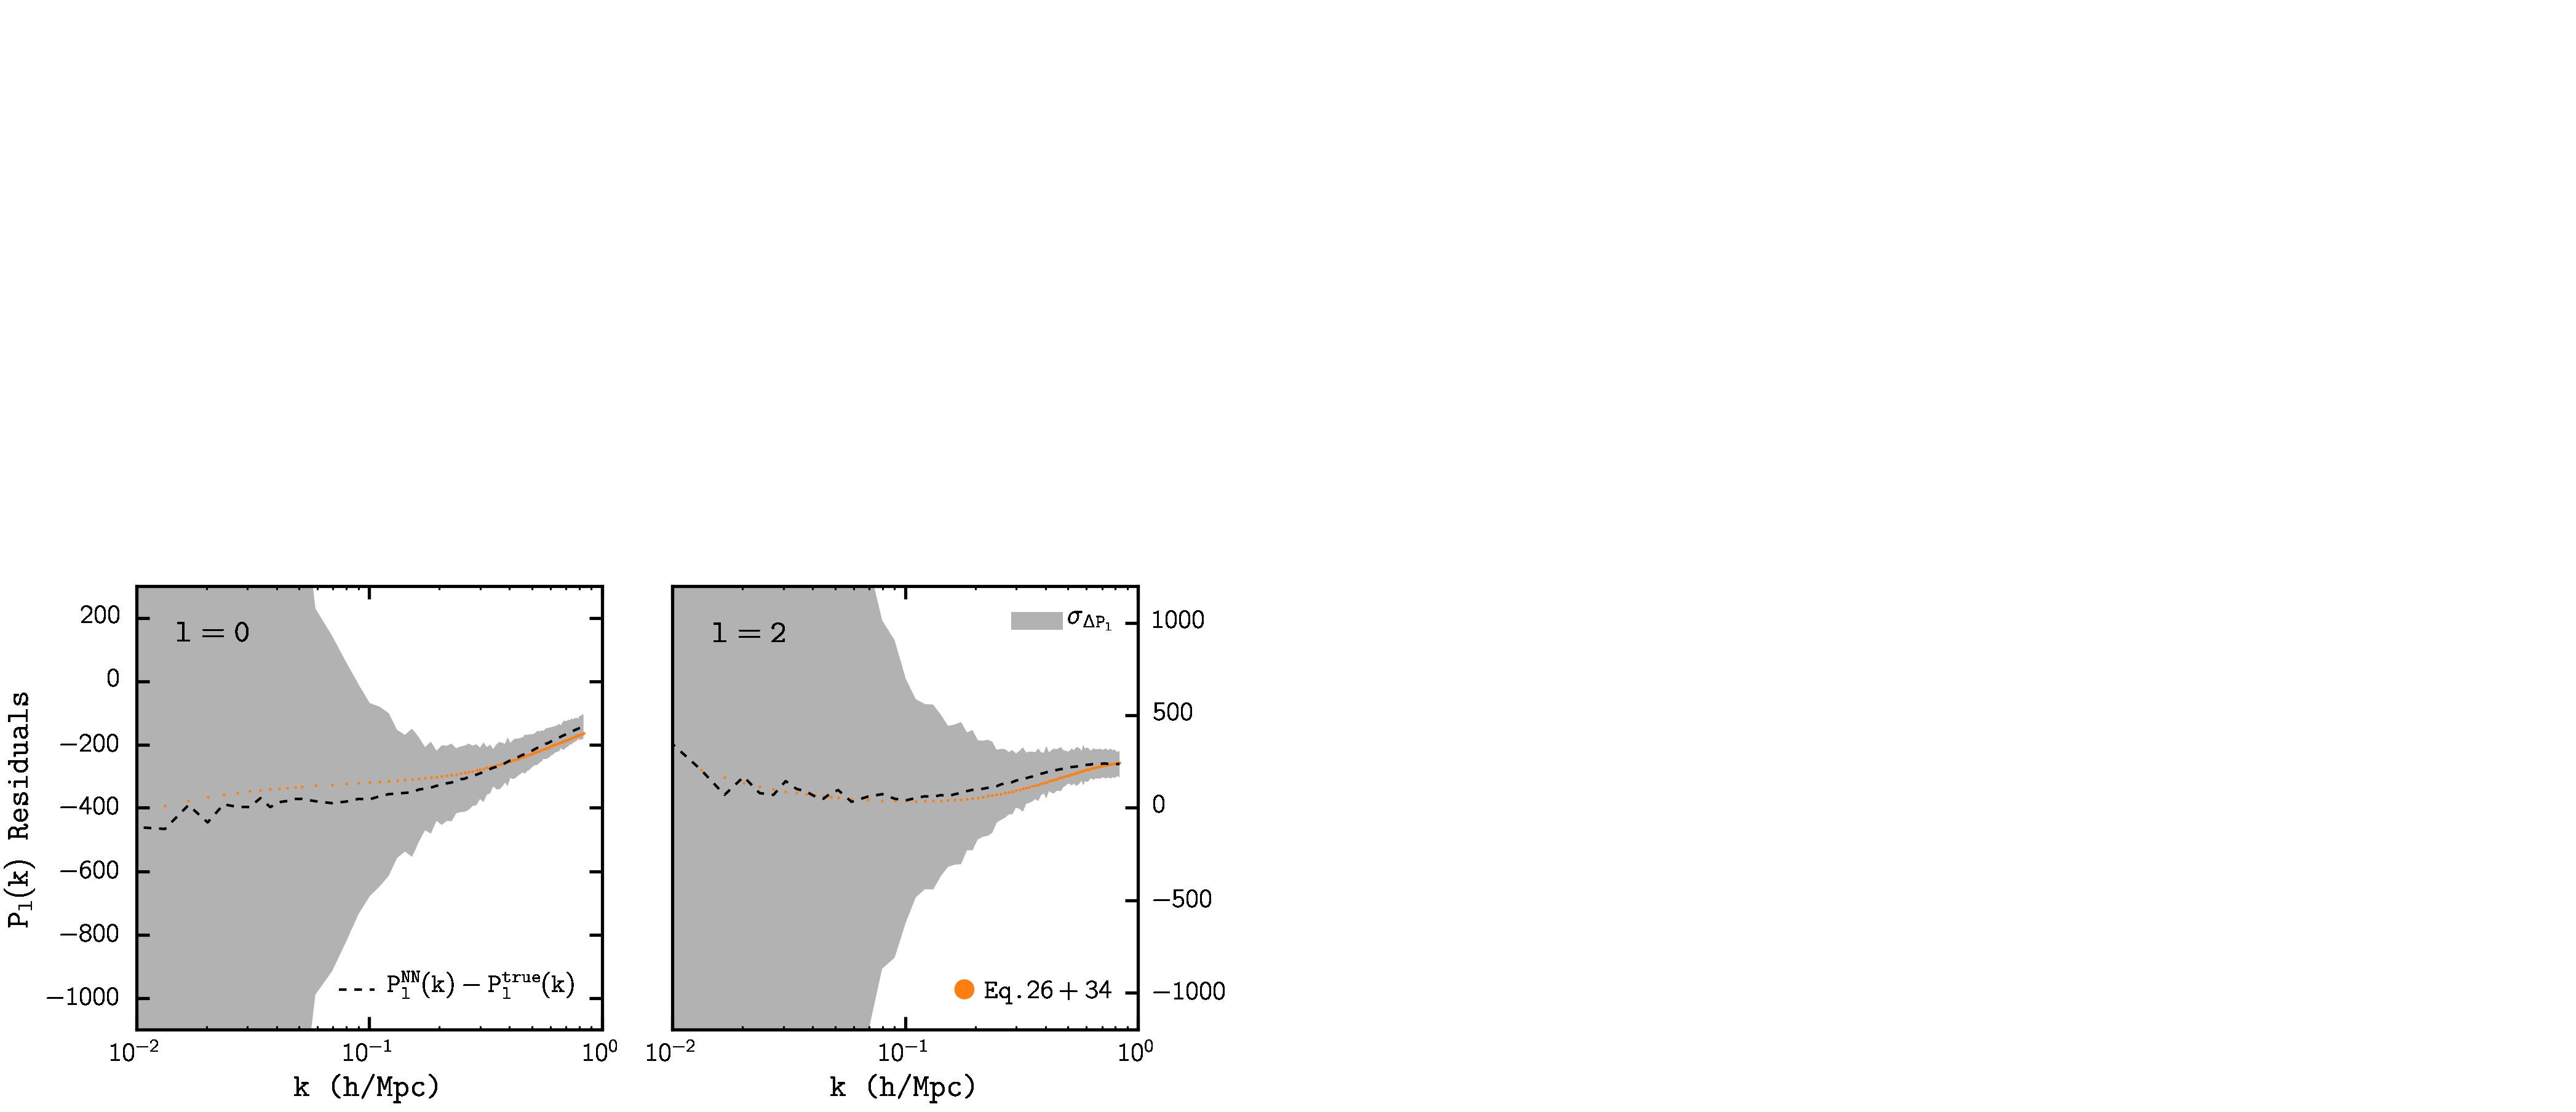
\includegraphics[width=1.\textwidth]{figs/fc/mock_catalog_tophatconv_upw_delPlk_rebin6x.pdf}
\caption{Comparison of the power spectrum residuals from NN-corrected fiber collisions 
$\Delta P_l = P_l^\mathrm{NN} - P_l^\mathrm{true}$ (dashed black) with 
the $\Delta P_l$ from the effective window method obtained by adding Eqs.~(\ref{DeltaPellUC}) and~(\ref{DeltaPell2}) (\nseriescolor) for the monopole (left)
and quadrupole (right). The standard deviation of the power spectrum residual, 
$\sigma_{\Delta P_l}$, for the Nseries mock catalogs is shaded in gray.}
\label{fig:delP}
\end{center}
\end{figure*}
%%%%%%%%%%%%%%%%%%%%%%%%%%%%%%%%%%%%%%%%%%%%%%%%%%%%%%%%%%%%%%%%%%%%%%%%%%%%%%%%


The first term, $\Delta P^\mathrm{uncorr}$, can be easily obtained:
\begin{align} \label{eq:delp_uncorr}
\Delta P^\mathrm{uncorr} &=  - f_s\, \widehat{W_\mathrm{fc}}({\bf k}) = 
-f_s \int e^{i {\bf k} \cdot {\bf r}} \: W_\mathrm{fc}({\bf r}) \, d^3{r} \nonumber \\
& = -f_s \ 2 \pi \delta_D(k_\parallel) \; \pi D_\mathrm{fc}^2 \; W_\mathrm{2D}(k_\perp D_\mathrm{fc}). 
\end{align}
where $W_\mathrm{2D}(x) \equiv 2 J_1(x)/x$ is the top-hat function in 2D (a cylinder), and 
$J_1$ is a Bessel function of the first kind and of order $1$. The multipole 
contributions of Eq.~(\ref{eq:delp_uncorr}) are then 
\beqa
\Delta P^\mathrm{uncorr}_l(k) & = & -f_s \  (2l+1) \mathcal{L}_l(0) \,  {(\pi D_\mathrm{fc})^2 \over k} \;  W_\mathrm{2D}(k D_\mathrm{fc}),
\nonumber \\ & & 
\label{DeltaPellUC}
\eeqa
where ${\cal L}_l$ are the Legendre polynomials. The $k^{-1}$ prefactor here, arising from the delta function in Eq.~(\ref{eq:delp_uncorr}) is an approximation for scales smaller than the survey size, since the delta function follows from assuming we can integrate up to infinity along the line of sight in Eq.~(\ref{eq:delp_uncorr}).
Equation~(\ref{DeltaPellUC}) gives a correction that alternates in sign as a function of multipole $l$.
Note that since for practical purposes $k D_\mathrm{fc} \ll 1$, we can expand 
\beqa
\Delta P^\mathrm{uncorr}_l(k)  &= & -f_s \pi D_\mathrm{fc}^2  \,  \Big({2\pi \over k}\Big) \ {(2l+1) \over 2}\, \mathcal{L}_l(0) \nonumber \\
& & \times \Big(1 - \frac{(k D_\mathrm{fc})^2}{8} + \ldots \Big),
\label{DeltaPuncorrexp}
\eeqa
% note  the leading order term is independent of type of window assumed!
and for scales involved in typical analysis the first term suffices, which means that the uncorrelated piece of fiber collisions decays as $k^{-1}$ across the relevant range of scales. The magnitude of this uncorrelated  effect (chance collisions) is small, given by the effective survey area affected by fiber collisions $f_s \pi D_\mathrm{fc}^2$ times the wavelength of perturbations $2\pi/k$.

For the correlated piece $\Delta P^\mathrm{corr}$, we see from Eqs.~(\ref{eq:tophat_pk}) and~(\ref{eq:delp_uncorr})  that we need $W_\mathrm{2D}(|{\bf k}_\perp -{\bf q}_\perp| D_\mathrm{fc})$ for which we can use the addition theorem for 2D top-hat functions~\citep{Bernardeau:2002aa},
\beqa
W_\mathrm{2D}(|{\bf k}_\perp -{\bf q}_\perp| D_\mathrm{fc}) &=& \sum_{k=0} (k+1)\, U_k(\hat{k}_\perp\cdot \hat{q}_\perp) \nonumber
\\ & & W_\mathrm{2D}^{(k/2)}(k_\perp D_\mathrm{fc}) \,
W_\mathrm{2D}^{(k/2)}(q_\perp D_\mathrm{fc}) \nonumber \\ & & 
\label{ADDtheo}
\eeqa
where the $U_k$'s are the Chebyshev polynomials and $W_\mathrm{2D}^{(k/2)}(x) \equiv 2J_{k+1}(x)/x$. Now, again, as we are interested in scales for which $k D_\mathrm{fc} \ll 1$ is an excellent approximation, dropping ${\cal O}(k_\perp D_\mathrm{fc})^2$ we can just use the $k=0$ term in this expression. This gives us $W_\mathrm{2D}(|{\bf k}_\perp -{\bf q}_\perp| D_\mathrm{fc}) \approx W_\mathrm{2D}( q_\perp D_\mathrm{fc})$ as expected and leads to,
\beqa
\Delta P^\mathrm{corr}({\bf k}) &\approx& -{f_s \pi D_\mathrm{fc}^2}\int {d^2q_\perp\over (2\pi)^2} \, P(k_\parallel,q_\perp) \, W_\mathrm{2D}( q_\perp D_\mathrm{fc}) \nonumber \\ & &  \label{eq:delp_corr}
\eeqa
This is a simple result, showing that the correlated effect of fiber collisions is  proportional to the effective survey area affected by fiber collisions and to the  integral of the power spectrum over 2D modes perpendicular to the line of sight smoothed at the fiber collision scale. 
The multipole components of Eq.~(\ref{eq:delp_corr}) are, after expanding $P(k_\parallel,q_\perp)$ in multipoles,
\beq
\Delta P^\mathrm{corr}_l(k) \approx -\frac{f_s D_\mathrm{fc}^2}{2} \sum_{l'=0}^\infty \int_0^\infty q dq P_{l'}(q) \, f_{l l'}(k,q), 
\label{DeltaPell}
\eeq
where, again neglecting ${\cal O}(k D_\mathrm{fc})^2$,
\beqa
f_{ll'}(k,q) &\equiv &
\Big(\frac{2l+1}{2}\Big) \int_{\mathrm{max}(-1,-q/k)}^{\mathrm{min}(1,q/k)} d\mu  \, {\cal L}_l(\mu)\, {\cal L}_{l'}(k\mu/q) \nonumber \\ & &
\  \ \ \ \ \ \ \ \ \ \ \ \ \times \ W_\mathrm{2D}( q\, D_\mathrm{fc})
\label{fellellp}
\eeqa
This has a simple expression for $l=l'$,
\beq
f_{ll}(k,q) = f_*(k,q)\, W_\mathrm{2D}( q\, D_\mathrm{fc})\, \Big(\frac{k_<}{k_>}\Big)^l
\label{fdiag}
\eeq
where $f_*(k,q)=q/k$ for $q\leq k$ and unity otherwise, and $k_>=\mathrm{max}(k,q)$ and $k_<=\mathrm{min}(k,q)$. On the other hand, off the diagonal we have ($l \neq l'$)
\beq
f_{ll'}(k,q) = f_*(k,q)\, W_\mathrm{2D}( q\, D_\mathrm{fc})\, \Big(\frac{2l+1}{2}\Big) \,H_{l_>l_<}\Big(\frac{k_<}{k_>}\Big),
\label{foffdiag}
\eeq
where $l_{>}=\mathrm{max}(l,l')$ and similarly $l_<$, and  $H_{l_>l_<}(x)$ is a polynomial of degree $l_>$ which vanishes unless $l$ and $k$ are both larger or  smaller than $l'$ and $q$ respectively. The first few polynomials are listed in the Appendix~\ref{chap:append1}. Since $f_{l>l'}(k<q) = f_{l<l'}(k>q)=0$ it is convenient to split the integrals depending on whether $q$ is larger or smaller than $k$, which leads to
\beqa
\Delta P^\mathrm{corr}_l(k) &\approx & -\frac{f_s D_\mathrm{fc}^2}{2} \Bigg[\,
\sum_{l'\leq l} \int_0^k q dq \, P_{l'}(q) \, f_{l l'}(q\leq k) \nonumber \\ & & + 
\sum_{l'\geq l} \int_k^\infty q dq\, P_{l'}(q) \, f_{l l'}(q\geq k) \Bigg],
\label{DeltaPell2}
\eeqa
which shows that the change of power spectrum multipole $l$ due to correlated 
fiber collisions comes from long modes of lower multipoles ($l'\leq l$) and 
short modes of higher multipoles ($l'\geq l$). Going back to the results 
displayed in Figure~\ref{fig:2pcf_tophat}, we can now formulate how our results 
change if we use the observed numerical profile in the right panel of 
Figure~\ref{fig:2pcf_tophat} (red line) instead of the top-hat (black dashed). 
One can check that to leading order in $k D_\mathrm{fc}$, which is all we are using in this paper, our expression for the uncorrelated and correlated change in power are valid as long as we replace the 2D top-hat by the numerical profile in Eq.~(\ref{fellellp}), and redefine the scale $D_\mathrm{fc}$ that appears in Eqs.~(\ref{DeltaPuncorrexp}) and~(\ref{DeltaPell}) from the area of the numerical profile, that is 
\beq
\int d^2r_\perp \, W_\mathrm{2D}({\bf r}_\perp) \equiv \pi\, D_\mathrm{fc}^2
\label{redefDfc}
\eeq

%
%\begin{align} \label{eq:delp_corr}
%\Delta P^\mathrm{corr}  
%&= -4 \pi^3 f_s D_\mathrm{fc}^2 \int P(k_\parallel \hat{e}_\parallel + q_\perp \hat{e}_\perp) \times \nonumber \\
%& \qquad \frac{J_1(D_\mathrm{fc}(k_\perp - q_\perp))}{D_\mathrm{fc}(k_\perp - q_\perp)}
%\;\frac{\mathrm{d}^3q}{(2\pi)^3} \nonumber \\
%&= - \frac{f_s D_\mathrm{fc}^2}{2} \int q_\perp P(k_\parallel \hat{e}_\parallel + q_\perp \hat{e}_\perp) \times \nonumber \\
%& \qquad W_\mathrm{1D} \left(k_\perp D_\mathrm{fc}, \; q_\perp D_\mathrm{fc} \right) \; \mathrm{d}q_\perp
%\end{align}
%where 
%\begin{align} \label{eq:w1d}
%W_\mathrm{1D}(x, \; y) = 
%\int\limits_{0}^{2\pi} \frac{J_1(\sqrt{x^2 + y^2 - 2 x y\;cos \phi})}
%{\sqrt{x^2 + y^2 - 2 x y\;cos \phi}}\; \frac{\mathrm{d}\phi}{2\pi}.
%\end{align}
%The multipole components of Eq. \ref{eq:delp_corr} are 
%\begin{align}
%\Delta P^\mathrm{corr}_l(k) &= -\frac{f_s D_\mathrm{fc}^2}{2} \; 
%\left(\frac{2l+1}{2} \right)  \bigg[
%\int\limits_{-1}^{1} \mathrm{d}\mu\;\mathcal{L}_l(\mu) 
%\int\limits_{0}^{\infty} q_\perp\mathrm{d}q_\perp \nonumber \\
%& P(k\mu\;\hat{e}_\parallel + q_\perp \hat{e}_\perp) \;
%W_\mathrm{1D} \left(k\sqrt{1 - \mu^2} D_\mathrm{fc}, 
%\; q_\perp D_\mathrm{fc} \right) \; 
%\bigg]
%\end{align}
%
%\noindent Since $q = \sqrt{k^2\mu^2+q_\perp^2}$, the integral can be rearranged to  
%\begin{align} \label{eq:pkmu_delpcorr}
%\Delta P^\mathrm{corr}_l(k) 
%&= -\frac{f_s D_\mathrm{fc}^2}{2} \; \left(\frac{2l+1}{2} \right)\bigg[
%\int\limits_{0}^{\infty} q\; \mathrm{d}q
%\int\limits_{\mathtt{max}(-1, \frac{q}{k})}^{\mathtt{min}(1, \frac{q}{k})} \mathrm{d}\mu \; \mathcal{L}_l(\mu) \times \nonumber \\ 
%& P(q, \frac{k\mu}{q})\; W_\mathrm{1D} \left(k D_\mathrm{fc} \sqrt{1 - \mu^2}, 
%\; q D_\mathrm{fc} \sqrt{1 - \frac{k^2\mu^2}{q^2}} \right)\bigg]
%\end{align} 
%From $P(k, \mu)$, we can calulate both $\Delta P_l^\mathrm{corr}$ and 
%$\Delta P_l^\mathrm{uncorr}$. In other words, we can model the effect of 
%fiber collisions on the power spectrum monopole and quadrupole from $P(k, \mu)$. 

                                                                                                                                                                                                                                                                            %%%%%%%%%%%%%%%%%%%%%%%%%%%%%%%%%%%%%%%%%%%%%%%%%%%%%%%%%%%%%%%%%%%%%%%%%%%%%%%%
                                                                                                                                                                                                                                                                            % Del P Untrusted comparison figure  
                                                                                                                                                                                                                                                                            %%%%%%%%%%%%%%%%%%%%%%%%%%%%%%%%%%%%%%%%%%%%%%%%%%%%%%%%%%%%%%%%%%%%%%%%%%%%%%%%
\begin{figure*}
\begin{center}
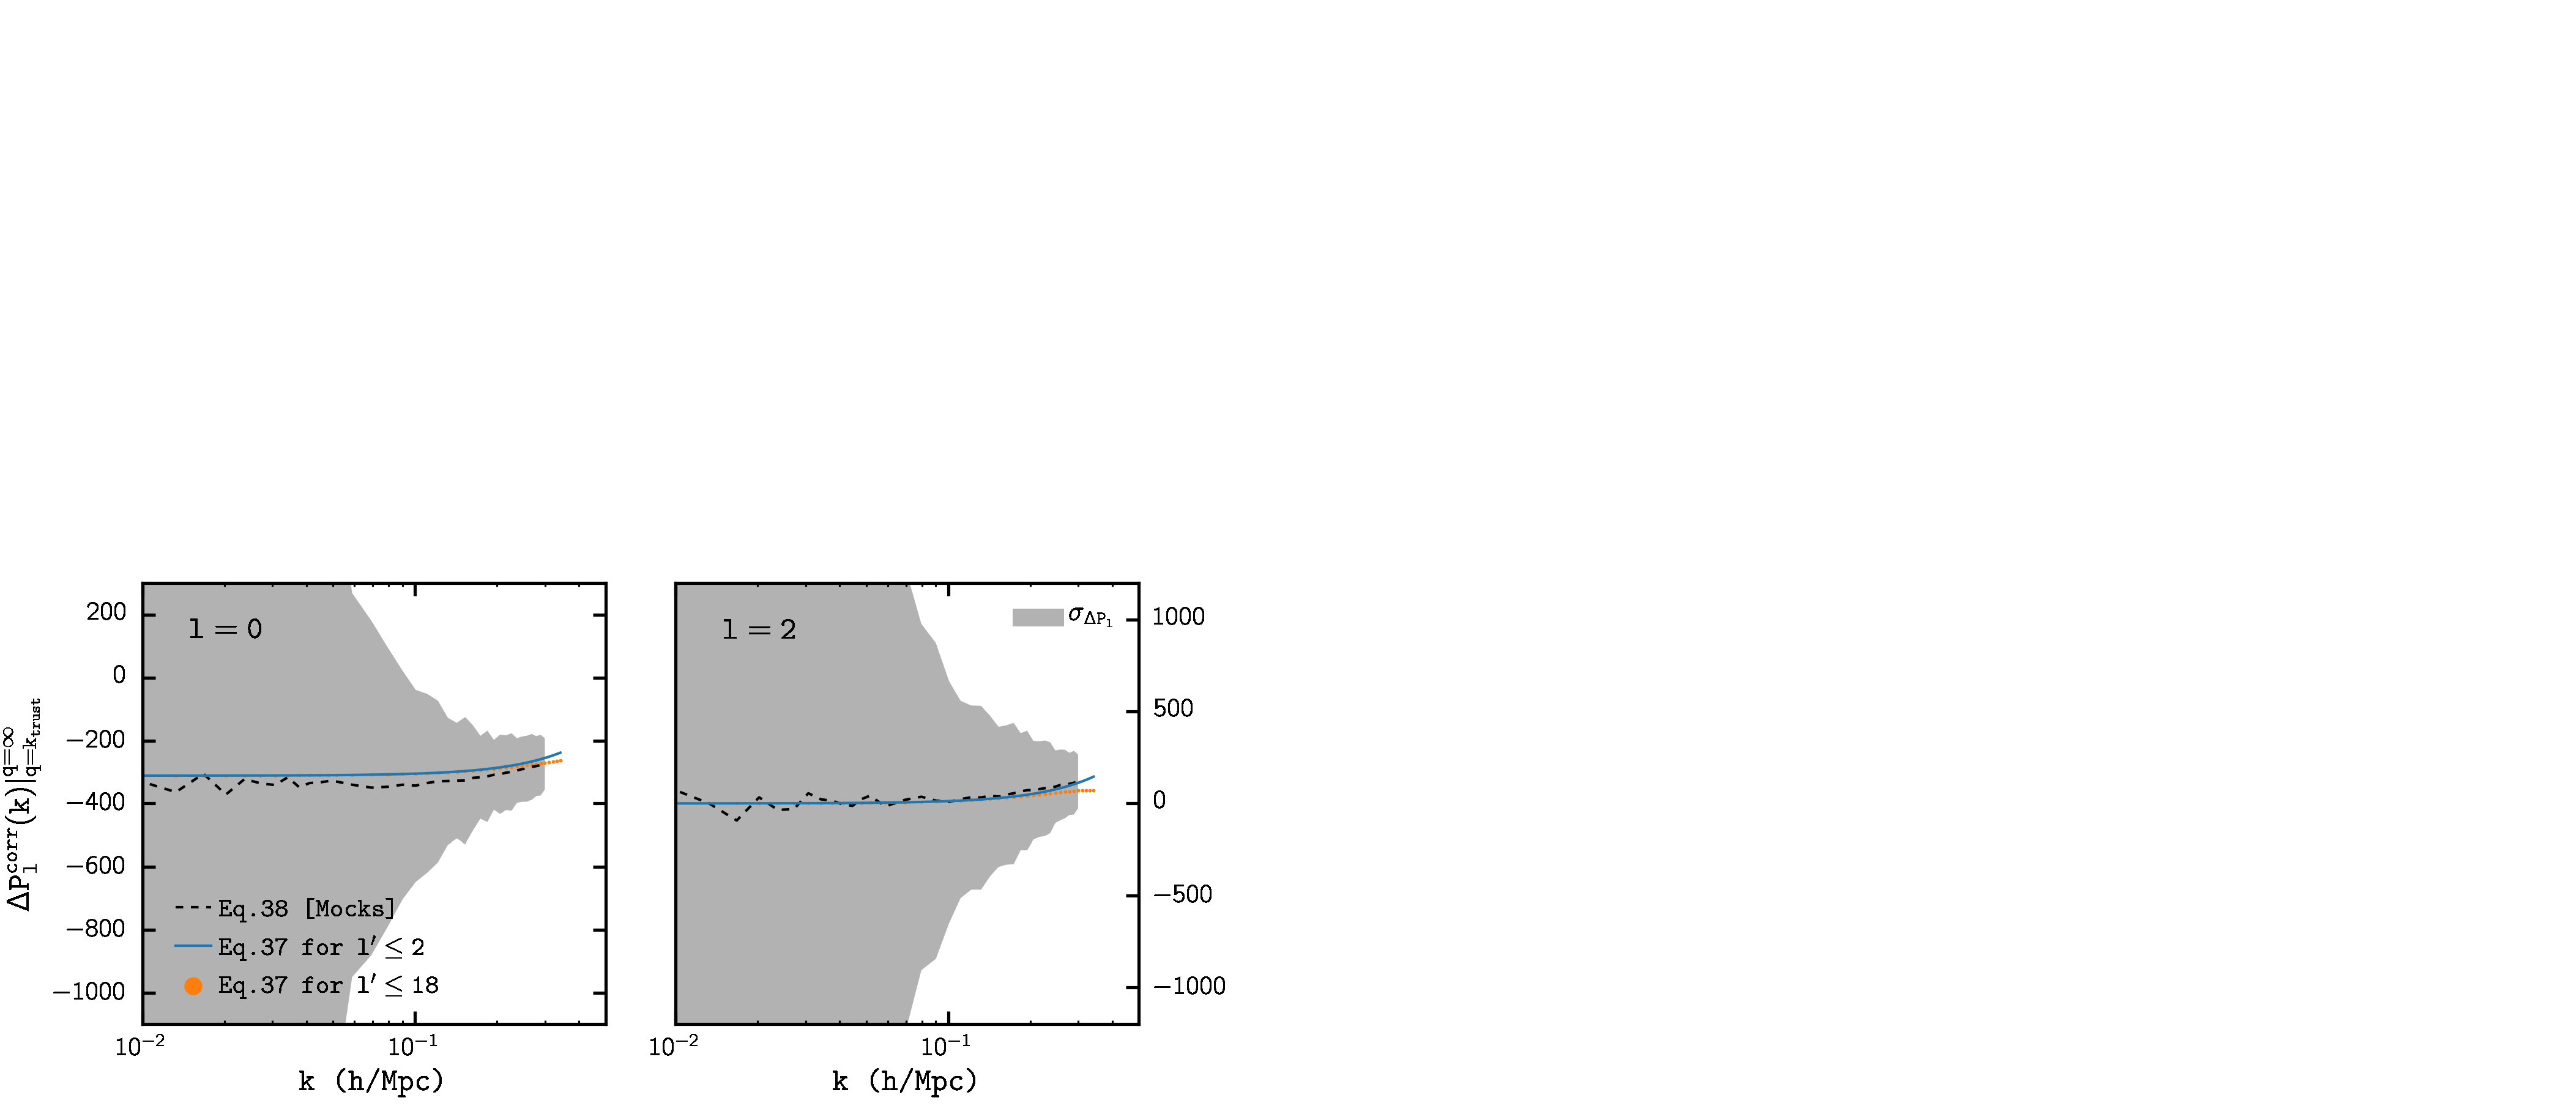
\includegraphics[width=1.\textwidth]{figs/fc/mock_catalog_tophatconv_delPlk_untrusted_18_rebin6x.pdf}
\caption{Comparison of the correlated power spectrum residuals from unreliable modes obtained from mocks (dashed), Eq.~(\ref{eq:delp_untrust_nseries}), 
to the polynomial approximation of  
Eq.~(\ref{eq:delp_poly}) for $l' \leq 18$ (orange). The left and right panels
correspond to $l = 0$ and $2$ respectively. The gray shaded region is the 
standard deviation for the Nseries $(P_l^\mathrm{NN} - P_l^\mathrm{true})$.  
We also include Eq.~(\ref{eq:delp_poly}) evaluated only for $l' \leq 2$ (blue). 
The agreement between Eq.~(\ref{eq:delp_poly}) for $l' \leq 2$ and Eq.~(\ref{eq:delp_untrust_nseries}) demonstrate that while higher orders of $l'$ are 
necessary to properly model $\Delta P_l^\mathrm(k)$ at higher $k$ values, 
for $k < k_\mathrm{trust}$ ($0.3\;h/\mathrm{Mpc}$ above) $l' \leq 2 $ are 
sufficient.}
\label{fig:delP_untrust}
\end{center}
\end{figure*}
%%%%%%%%%%%%%%%%%%%%%%%%%%%%%%%%%%%%%%%%%%%%%%%%%%%%%%%%%%%%%%%%%%%%%%%%%%%%%%%%


We now proceed to testing these results, for which we need the true power spectrum multipoles down to small scales to feed into Eq.~(\ref{DeltaPell2}). Unfortunately, in the nonlinear regime the multipole expansion is not very efficient (in the sense that the amplitude of multipoles does not decrease sharply with increasing multipole), so a large number of multipoles $l'$ is required to capture the contribution from small scale modes.  Measuring multipoles higher than the hexadecapole for realistic survey geometries  using our estimator becomes expensive due to the number of 
Fast Fourier Transforms (FFTs) that needs to be computed, and even for the most efficient version of the multipole estimators that requires only 7 FFTs one would worry about increased cosmic variance (see discussion in \citealt{Scoccimarro:2015aa}). 

A more efficient approach is to use the Nseries simulation boxes to test Eqs.~(\ref{eq:delp_uncorr}) and~(\ref{DeltaPell2}). The Nseries simulation boxes are the 
original simulations where the Nseries mocks were 
cut out from (Section \ref{sec:catalog}). Since the Nseries mocks 
are cut outs of the boxes, 
discrepancies in their power spectra are caused by the BOSS survey 
geometry and occur mainly at the largest scales, $k < 0.05\;h/\mathrm{Mpc}$ \citep{Beutler:2014aa,Grieb:2016aa}. 
At smaller scales, the difference between the power spectrum monopole, 
quadrupole and hexadecapole of Nseries mocks versus the Nseries boxes are 
negligible. 
Therefore, we calculate the $P_{l'}(q)$ from the Nseries simulation box, 
using periodic boundary conditions, which only requires one FFT and go up to $q = 43.5\;h/\mathrm{Mpc}$ and $l'=18$ to compute the corrections predicted by  Eq.~(\ref{DeltaPell2}).  

In Figure \ref{fig:delP}, we compare $\Delta P_l = \Delta P_l^\mathrm{corr} + 
\Delta P_l^\mathrm{uncorr}$ calculated from the Nseries Box power spectrum multipoles using Eqs.~(\ref{eq:delp_uncorr}) and~(\ref{DeltaPell2}) (\nseriescolor) to the Nseries mock catalogs power spectrum residuals, $\Delta P_l = P_l^\mathrm{NN} - P_l^\mathrm{true}$ (dashed). 
The left panel compares the monopoles ($l = 0$) while the right panel compares 
the quadrupoles ($l=2$). We also include in the gray shaded 
region, the standard deviation of Nseries mock catalogs power spectrum residuals,
$\sigma_{\Delta P_l}$. For both the monopole and quadrupole, the predictions (orange) agree with the measured residuals from NN-corrected fiber collisions (dashed black) well within the errors throughout the probed $k$ range up to $k=0.83\;h/\mathrm{Mpc}$. At low-$k$, the downturn (upturn) in the monopole (quadrupole) is due to the contribution of the $k^{-1}$ uncorrelated piece. 
The overall quality of the  agreement demonstrates that the effective window method can be used to robustly 
estimate the effect of fiber collisions on $P_l(k)$. Furthermore, with its
excellent performance for the quadrupole, the effective window approach 
provides an improvement over the LOS reconstruction method (Section
\ref{sec:dlospeak}). 

%%%%%%%%%%%%%%%%%%%%%%%%%%%%%%%%%%%%%%%%%%%%%%%%%%%%%%%%%%%%%%%%%%%%%%%%%%%%%%%%
% Tophat Convolution in Practice
%%%%%%%%%%%%%%%%%%%%%%%%%%%%%%%%%%%%%%%%%%%%%%%%%%%%%%%%%%%%%%%%%%%%%%%%%%%%%%%%
\subsubsection{In Practice} \label{sec:tophat_practice}
There are, however, practical limitations to the effective window model 
as it described above. The 
$\Delta P^\mathrm{corr}_l$ calculations in 
Eq.~(\ref{DeltaPell2}) involves integrating the power spectrum over the $q$
range of $0$ to $\infty$. While this integral converges for $q \approx10\;h/\mathrm{Mpc}$ 
for both monopole and quadrupole, in practice one cannot compute reliably the power spectrum multipoles down to these scales. We now 
discuss a way to overcome this issue.

Let $k_\mathrm{trust}$ represent the scale up to which we can calculate reliably power 
spectrum multipoles. We therefore split the second term in Eq.~(\ref{DeltaPell2}) 
into a reliable piece (integration from $k$ to $k_\mathrm{trust}$) and an 
unreliable piece (integration from $k_\mathrm{trust}$ to $\infty$), so schematically
\beq \label{eq:delp_split}
\Delta P^\mathrm{corr}_l =  \Delta P^\mathrm{corr}_l \bigg|_{q=0}^{q=k_\mathrm{trust}} +  
\Delta P^\mathrm{corr}_l \bigg|_{q=k_\mathrm{trust}}^{q=\infty}.
\eeq
The first term can be reliably calculated from first principles 
since it involves modes from $q=0$ to $q=k_\mathrm{trust}$ and corresponds to  the first term  plus the reliable piece of the second term in Eq.~(\ref{DeltaPell2}). Now, the key fact is that because the second term in Eq.~(\ref{eq:delp_split}) only depends on $k$ through $f_{l l'}(q\geq k)$, from Eqs.~(\ref{fdiag}-\ref{foffdiag}) it follows that the $k$-dependence of the unreliable term is simply a polynomial in $k$,

\begin{align} \label{eq:delp_poly}
\Delta P^\mathrm{corr}_l \bigg|_{q=k_\mathrm{trust}}^{q=\infty} &= 
\sum\limits_{n= 0, 2, 4 ... } C_{l,n}\;k^{n}. 
\end{align}
The coefficients of the polynomial, $C_{l, n}$, are obtained by collecting powers of $k$ from the sum over the $H$-polynomial contributions to the second term in Eq.~(\ref{DeltaPell2}). How important are these unreliable contributions? In order to test this, in Figure \ref{fig:delP_untrust} 
we calculate $C_{l, n}$ from the $P_{l'}(q)$ multipoles measured 
from the Nseries simulation boxes (blue and orange for terms up 
                                                                                                                                                                                                                                                                            to $l'=2$ and $18$ respectively) and compare to (black dashed)
\beq \label{eq:delp_untrust_nseries}
    \Delta P_l^\mathrm{Nseries}(k) - \Delta P^\mathrm{uncorr}_l(k) - 
    \Delta P^\mathrm{corr}_l(k) \bigg|^{q=k_\mathrm{trust}}_{q=0}
\eeq  
where $\Delta P_l^\mathrm{Nseries}$ is the power spectrum 
residual $P_l^\mathrm{NN}- P_l^\mathrm{true}$ for the Nseries mocks (Figure \ref{fig:delP}). We once again include the standard deviation 
of the power spectrum residual in shaded gray. The agreement 
between Eq.~(\ref{eq:delp_poly}) and Eq.~(\ref{eq:delp_untrust_nseries}) 
is more or less equivalent to the agreement seen in Figure~\ref{fig:delP}, which includes uncorrelated and reliable correlated contributions as well; this 
should of course not come as a surprise.

More importantly, when we examine the contribution to 
$\Delta P^\mathrm{corr}_l |_{k_\mathrm{trust}}^\infty$ from each individual 
$l'$ order term of the Eq.~(\ref{eq:delp_poly}) polynomial, we find that the
main contributors at $k < k_\mathrm{trust} \sim 0.3\; h/\mathrm{Mpc}$ are 
the $l' \leq 2$ order terms. In fact, the higher order ($l' > 2$) terms of the 
polynomial contribute at higher $k$. For instance, the $l' = 4, 6,$ and $ 8$ terms 
only begin to significantly contribute at scales of $k > 0.3, \; 0.45$, and 
$0.6\;h/\mathrm{Mpc}$ respectively, which is not surprising since higher $k$ powers come together with increasing inverse powers of $q$ and thus suppress the value of the coefficients that result from integrating over small-scale modes. Hence, when we plot Eq.~(\ref{eq:delp_poly})  
for just $l' \leq 2$ (blue) in Figure~\ref{fig:delP_untrust}, we find that 
it is in good agreement with both Eq.~(\ref{eq:delp_poly}) for $l' \leq 18$ 
and Eq.~(\ref{eq:delp_untrust_nseries}). We also note that for $l = 2$, 
$C_{2, l'=0} = 0$ so the main contribution to 
$\Delta P^\mathrm{corr}_2(k < k_\mathrm{trust}) |_{k_\mathrm{trust}}^\infty$ 
comes solely from the $l' = 2$ term of the polynomial. 

To use the effective window method for cosmological inference, we can 
utilize the fact that Eq.~(\ref{eq:delp_poly}) with only $l' \leq 2$ terms 
provides an accurate estimate of the unreliable correlated change in power (Figure~\ref{fig:delP_untrust}). In cosmological analyses, the coefficients $C_{l, 0}$ and $C_{l, 2}$
can be nuisance parameters with priors obtained from  
mock catalogs. More specifically, for the quadrupole, since $C_{2, 0} = 0$
only one nuisance parameter is necessary. Meanwhile 
for the monopole, a constant shot noise term is typically already included as
a nuisance parameter in the analysis (\citealt{Beutler:2014aa,Beutler:2016aa,Grieb:2016aa,Gil-Marin:2016aa}) so there is 
also only one extra nuisance parameter for $l=0$. Therefore, 
by adding $C_{l, 2}$ as nuisance parameters to cosmological inference 
analyses of the power spectrum multipoles, we can use the effective window 
method to robustly marginalize over the effects of fiber collision for the 
entire $k$ range of power spectrum models based on perturbation theory. 

%\todo{ May be Fig.10 shows that the extra $k^2$ terms are not needed? They look like small contributions, most $k^2$ dependence seems to be from the reliable correlated piece. Can we just calculate $k_{\chi^2}$ for the CM (convolution method) without the $k^2$ terms but correct $k^0$ shot noise? It'd be nice to see what $k_{\chi^2}$ is for the CM and put this method in the same footing as NN and LRec.}
%%%%%%%%%%%%%%%%%%%%%%%%%%%%%%%%%%%%%%%%%%%%%%%%%%%%%%%%%%%%%%%%%%%%%%%%%%%%%%%%
% Summary and Discussion  
%%%%%%%%%%%%%%%%%%%%%%%%%%%%%%%%%%%%%%%%%%%%%%%%%%%%%%%%%%%%%%%%%%%%%%%%%%%%%%%%
\section{Summary and Conclusions} \label{sec:summary}
Using simulated mock catalogs designed specifically for interpreting BOSS 
clustering measurements with realistically imposed fiber collisions, we 
demonstrate that the Nearest Neighbor method (NN), most common used for dealing 
with fiber collisions, is insufficient in accounting for the effect of 
fiber collisions on the galaxy power spectrum monopole and quadrupole.  
Although fiber collisions have little significant effect on 
the power spectrum at large scales, their effect quickly overtakes sample 
variance on scales smaller than $k \approx 0.1 \;h/\mathrm{Mpc}$. At  $k \sim 0.3 \;h/\mathrm{Mpc}$
fiber collisions have over a $7.3\%$ and $73\%$ 
impact on the power spectrum monopole and quadrupole, respectively. The 
effect is equivalent to $7.3$ and $2.5$ times the sample variance of CMASS for 
$\delta k \approx 0.01\;h/\mathrm{Mpc}$, leading to a binning-independent scale of validity of the NN method of 
$k_{\chi^2}=0.068\;h/\mathrm{Mpc}$ for the monopole and $k_{\chi^2}=0.17\;h/\mathrm{Mpc}$ for the 
quadrupole (see bottom panel of Figure~\ref{fig:dlospeak_norm_resid}).  
Consequently at these scales, measurements of the power spectrum becomes 
dominated by the systematic effects of fiber collisions. 

Some recent methods (\citealt{Beutler:2014aa,Gil-Marin:2014aa,Beutler:2016aa,Grieb:2016aa,Gil-Marin:2016aa}) have supplemented
the NN method with adjustments to the constant shot noise term in the power spectrum 
estimator. While these methods improve the overall residual for the monopole, e.g. $k_{\chi^2}=0.17\;h/\mathrm{Mpc}$ for the method by \cite{Gil-Marin:2014aa}, they fail to account for the $k$-dependence of the systematic effect on smaller 
scales. Furthermore, since the quadrupole does not have a shot 
noise term, these methods provide no improvements for $l \geq 2$. 

In this paper, we first model the distribution of the line-of-sight displacement between 
fiber collided pairs using  mock catalogs. From the model, we statistically reconstruct the 
clustering of fiber collided galaxies that reside in the same halo. This, combined with the actual shot noise subtraction   
of the power spectrum estimator that accounts for chance alignments, 
leads to our LOS Reconstruction method that recovers very well the true power 
spectrum monopole from fiber collided data. As an added advantage, the method 
only relies on parameters ($\sigma_\mathrm{LOS}$ and $f_\mathrm{peak}$) 
measured from the actual observations. This makes the performance of the method 
independent from the accuracy of the mock catalogs, which are known to be unreliable 
at small scales. 

Using the LOS Reconstruction method, we can recover the true power 
spectrum monopole to scales well beyond previous methods. The LOS Reconstruction monopole power spectrum residuals remain within sample 
variance until $k \sim 0.53\;h/\mathrm{Mpc}$ and $k_{\chi^2}$ extends to  
$0.29\;h/\mathrm{Mpc}$. However, for the power spectrum quadrupole
at $k = 0.2\;h/\mathrm{Mpc}$,
the LOS Reconstruction method only reduces the discrepancy between the 
fiber collided $P_2(k)$ and the true $P_2(k)$ to roughly the sample variance. 
Therefore, the true monopole power spectrum estimate from 
the LOS reconstruction method can be compared to the systematics free predicted  
power spectrum monopole to infer the cosmological parameters of interest without 
biases from fiber collisions, but for the quadrupole power spectrum the method is not a substantial improvement over previous methods. We trace this problem  to the fact that the quadrupole is more sensitive to the object by object finger of god effect, while the LOS reconstruction works only statistically starting from the distribution of close pairs. 

To improve on the LOS reconstruction results we develop the effective window method which, rather than attempting to correct the data before making measurements, computes theoretical predictions of the fiber-collided power spectrum multipoles.
In this approach, we approximate the effect that 
fiber collisions have on the two-dimensional configuration space two-point 
correlation function of the NN method as a scaled top-hat function. 
Then the effect of fiber collisions can be written as the sum of two contributions: 1) that of uncorrelated chance collisions, with an amplitude proportional to the 
the effective survey area affected by fiber collisions times the wavelength of perturbations, and 2) that of correlated collisions, which is also proportional to the effective survey area affected by fiber collisions and to the integral of the power spectrum over 2D modes perpendicular to the line of sight smoothed at the fiber collision scale.

Using high resolution mock catalogs, we demonstrate that our  analytic prescription 
accurately models the power spectrum residuals from the NN method to within sample variance of BOSS volumes  
at $k < 0.83\;h/\mathrm{Mpc}$ for both the monopole and quadrupole when the true power spectrum is known down to small scales from simulations, allowing to compute the fiber-collided predictions. Since typically we do not have fast reliable ways of computing the small scale power spectrum, we develop a practical approach when the power spectrum predictions are reliable up to some scale $k_\mathrm{trust}$. We split the contributions of the correlated fiber collisions effect into a  piece that can be calculated reliably as it depends on large-scale modes, and an unreliable piece that depends on modes that are not under control. We show that the latter piece can be written as polynomials in $k$, and demonstrate that for scales up to $k \sim 0.3\;h/\mathrm{Mpc}$, the unreliable contribution can be accurately estimated by a quadratic  polynomial in $k$. In principle, this method can be applied to larger $k_\mathrm{trust}$ than used here as a reasonable example ($k_\mathrm{trust} = 0.3\;h/\mathrm{Mpc}$). 

Therefore, using the effective window method we can model the fiber collided power 
spectrum as the systematics-free  power spectrum plus three contributions due to  
fiber collisions: an uncorrelated piece (independent of the model power spectrum), a calculable piece (which involves integrating the model power spectrum over 2D long-wavelength modes perpendicular to the line of sight), and an unreliable contribution that is a quadratic polynomial, $C_{l,0} + C_{l,2}\, k^2$. 
While the precise values of $C_{l, n}$ cannot be robustly predicted in practice 
because of its dependence on small scale power, the coefficients 
can be treated as nuisance parameters in the analysis. Typically a constant shot 
noise term is already included as a nuisance parameter, while the constant contribution vanishes for higher multipoles, therefore only one extra parameter 
per multipole is required (the $k^2$ corrections). For cosmological parameter inference, the fiber collided model power spectrum 
can be compared directly to the observed fiber 
collided power spectrum. Then by marginalizing over these free coefficients, we marginalize 
over the effect of small-scale power induced fiber collisions on the power spectrum, which allows us to robustly 
infer the cosmological parameters of interest.

The fiber collision correction methods we present will enable us to robustly 
account for the effects of fiber collisions in galaxy clustering analyses 
to the smallest scales allowed by theoretical predictions. They can also be extended to 
future surveys such as eBOSS  or any other large fiber-fed 
surveys that suffer from systematic effects of fiber collisions. Our fiber
collision correction method can also be extended to higher order clustering 
statistics such as bispectrum (Hahn et al., in prep.). We will use the methods 
presented in this paper to analyze the galaxy power spectrum and bispectrum 
multipoles in future work.

\section*{Acknowledgements}
CHH and MRB were supported by NSF-AST-1109432 and NSF-AST-1211644.
SRT is grateful for support from the Campus de Excelencia Internacional UAM/CSIC.
We thank A. I. Malz, Mohammadjavad Vakili, Johan Comparat and particularly 
David W. Hogg for helpful discussions. CHH also thanks the Instituto 
de F\'{i}sica Teo\'{o}rica (UAM/CSIC) and 
particularly Francisco Prada for their hospitality during his summer 
visit, where part of this work was completed.

\chapter{Parameter Inference \chaplabel{inference}}

\section{Standard Analysis}

\section{Covariance Matrix Estimation} % mock catalog calibration stuff

\seciton{Beyond Standard Inference} % ABC paper

%internal short cuts
\def \HgA {H$\gamma_A$}
\def \Hbp {H$\beta ^\prime$}
\def \lowenvthresh {0.0}
\def \highenvthresh {3.0}
\def \apradius{2.5}
\def \apheight{35}

\chapter{PRIMUS: Effects of Galaxy Environment on the Quiescent Fraction Evolution at \lowercase{\textit{z}}$<0.8$ \chaplabel{galenv}}


This \paper\ is joint work with Michael~R.~Blanton (NYU), John~Moustakas (Siena College), 
Alison~L.~Coil (UCSD), Richard J.~Cool (University of Arizona), Daniel J.~Eisenstein (Harvard),
Ramin A.~Skibb (UCSD), Kenneth C.~Wong (University of Arizona), and Guangtun~Zhu (Johns Hopkins Unviersity)
published in \emph{The Astrophysical Jounral} as \cite{Hahn:2015aa}. 

%%%%%%%%%%%%%%%%%%%%%%%%%%%%%%%%%%%%%%%%%%%%%%%%%%%%%%%%%%%%%%%%%%%%%%%%%%%%%%%%%%%%
% ABSTRACT
%%%%%%%%%%%%%%%%%%%%%%%%%%%%%%%%%%%%%%%%%%%%%%%%%%%%%%%%%%%%%%%%%%%%%%%%%%%%%%%%%%%%
\section{Chapter Abstract}
We investigate the effects of galaxy environment on the evolution of
the quiescent fraction ($f_{\mathrm{Q}}$) from $z =0.8 $ to $ 0.0$ using
spectroscopic redshifts and multi-wavelength imaging data from the
PRIsm MUlti-object Survey (PRIMUS) and the Sloan Digitial Sky Survey
(SDSS). Our stellar mass limited galaxy sample consists of $\sim
14,000$ PRIMUS galaxies within $z = 0.2-0.8$ and $\sim 64,000$ SDSS
galaxies within $z = 0.05-0.12$. We classify the galaxies as quiescent
or star-forming based on an evolving specific star formation cut, and
as low or high density environments based on fixed cylindrical
aperture environment measurements on a volume-limited environment
defining population. For quiescent and
star-forming galaxies in low or high density environments, we examine
the evolution of their stellar mass function (SMF). Then using the
SMFs we compute $f_{\mathrm{Q}}(\mathcal{M}_{*})$ and quantify its
evolution within our redshift range. We find that the quiescent
fraction is higher at higher masses and in denser environments. The
quiescent fraction rises with cosmic time for all masses and
environments. At a fiducial mass of $10^{10.5}M_\odot$, from $z\sim
0.7$ to $0.1$, the quiescent fraction rises by $15\%$ at the
lowest environments and by $25\%$ at the highest environments we measure.
These results suggest that for a minority of galaxies their cessation
of star formation is due to external influences on
them. In other words, in the recent Universe a substantial fraction of the
galaxies that cease forming stars do so due to internal processes.

%%%%%%%%%%%%%%%%%%%%%%%%%%%%%%%%%%%%%%%%%%%%%%%%%%%%%%%%%%%%%%%%%%%%%%%%%%%%%%%%%%%%
% INTRODUCTION
%%%%%%%%%%%%%%%%%%%%%%%%%%%%%%%%%%%%%%%%%%%%%%%%%%%%%%%%%%%%%%%%%%%%%%%%%%%%%%%%%%%%
\section{Introduction}
Galaxies, in their detailed properties, carry the imprints of their surroundings, with a strong dependence of the quiescent fraction of galaxies on their local environment (e.g. \citealt{hubble36a, oemler74a, dressler80a, hermit96a, guzzo97a}; for a recent review see \citealt{blanton09a}).  The strength of this dependence is itself a strongly decreasing function of galaxy stellar mass; at the extreme, the lowest mass ($<10^{9}$ $M_\odot$) galaxies end their star formation only in dense regions, and never in isolation (\citealt{geha12a}). These effects also vary with redshift at least in the densest clusters, as observed in the changing fraction of late-type spirals relative to the field, found in studies of the morphology-density relation (\citealt{dressler84a, Fasano:2000aa, Smith:2005aa, desai07a}). Clearly understanding the properties of galaxies in the present-day universe requires a careful investigation of the role of environment, and how that role changes over time.

%Moreover, at $z < 1$ lower star-formation rate early-type galaxies are found populating the denser regions (\citealt{cooper08a, patel09a, kovac10a}). 

Nevertheless, the evolution of the role of environment is a relatively subtle effect and must be interpreted within the context of the evolving galaxy population. For instance, the most dramatic change in galaxy properties during the past eight billion years has been the remarkable decline in the star-formation rate of galaxies in the Universe (\citealt{hopkins06a}). This decline appears dominated by decreases in the rates of star-formation of individual galaxies (\citealt{Noeske:2007aa}). There is evidence that a large fraction of the decline is associated with strongly infrared-emitting starbursts (\citealt{bell05a, magnelli09a}). As \cite{cooper08a} and others have pointed out, because the environmental dependence of total star-formation rates at fixed redshift is relatively small, environmental effects are unlikely to cause the overall star-formation rate decline.

During this period, the major classes of galaxies that we observe today have already been firmly in place (\citealt{bundy06a, borch06a, taylor09a, Moustakas:2013aa}). Though not as dramatic as the history of galaxies prior to $z \sim 1$, detailed observations of the stellar mass function find significant evolution of the galaxy population with the decline in the number density of massive star-forming galaxies accompanied by an increase in the number density of quiescent galaxies (\citealt{Blanton:2006ab, bundy06a,  borch06a, Moustakas:2013aa}). \cite{Moustakas:2013aa}, for instance, find that since $z \sim 1.0$ the $\sim 50\%$ decline in the number density of massive star-forming galaxies ($\mathcal{M}_{*} > 10^{11} \mathcal{M}_{\odot}$) is complemented by the rise in number density of intermediate-mass quiescent galaxies ($\mathcal{M}_{*} \approx 10^{9.5} - 10^{10}\mathcal{M}_{\odot}$), by a factor of $ 2-3$, and massive quiescent galaxies ($\mathcal{M}_{*} > 10^{11} \mathcal{M}_{\odot}$ ), by $\sim 20\%$. On the color-magnitude diagram, this corresponds to the doubling of the red sequence over this period (\citealt{Bell:2004aa, borch06a, Faber:2007aa}). These changes in galaxy population are likely a result of physical processes that cause the cessation of star-formation in star-forming galaxies. 

Of the numerous mechanisms that have been proposed to explain this cessation, favored models suggest that internal processes such as supernovae or active galactic nuclei heat the gas within the galaxy, which consequently suppresses the cold gas supply used for star-formation (\citealt{Keres:2005aa, Croton:2006aa, Dekel:2008aa}). Other models propose that environment dependent external processes such as ram-pressure stripping (\citealt{Gunn:1972aa, Bekki:2009aa}), strangulation (\citealt{Larson:1980aa, Balogh:2000aa}), or harassment (\citealt{Moore:1998aa}) contribute to the cessation. 

Observations such as \cite{Weinmann:2006aa} and \cite{Peng:2010aa} credit some of these proposed internal processes for the cessation of star-formation, especially in massive galaxies. Meanwhile, observations of galaxy properties such as color and morphology correlating with environment suggest that environment may play a role in ceasing star-formation (\citealt{blanton09a} and references therein). However, it remains to be determined whether the environmental trends in galaxy properties reflect the direct effect of external environment on the galaxies' evolution (e.g. ram pressure, tidal forces, mergers) or reflect statistical differences in the histories of galaxies in different environments (e.g. an earlier formation time in dense regions).

%However, it remains to be discerned whether these trends reflect the underlying differences among galaxy populations in different environments or if they are in fact effects of environment dependent external processes, which cause galaxies that would otherwise continue forming stars to cease their star-formation. 

%Similarly, a number of observations support the existence of environment dependent external processes (\citealt{Iovino:2010aa, geha12a, Kovac:2014aa}). \cite{Peng:2010aa} and others further argue that internal and external processes both contribute to the cessation of star-formation with internal processes more dominant in massive galaxies and external processes dominating the less massive regime. While discrepancies persist between theoretical models and observations, a large number of observations suggest that environment plays a significant role in ceasing star-formation. 

%Some of these proposed internal processes have received observational support. \cite{Weinmann:2006aa} and \cite{Peng:2010aa}, for example, credit internal processes for quenching star-formation, especially in massive galaxies. 

%Nevertheless, the evolution of the role of environment is a relatively subtle effect and difficult to study.  Although the history of galaxies prior to $z\sim 1$ appears to have been one of rapid assembly, since that time the galaxy population has continued to evolve, but less dramatically. Although there are detectable changes in the population, the major classes of galaxies existed at $z\sim 1$, in roughly the same relative numbers as today (\citealt{bundy06a, borch06a, taylor09a, Moustakas:2013aa}). Furthermore, at those redshifts we can also detect the dependence of galaxy properties on environment, with lower star-formation rate early-type galaxies populating the denser regions (\citealt{cooper08a, patel09a, kovac10a}).

%The most dramatic change in galaxy properties during the past eight billion years has been a remarkable decline in the star-formation rate of galaxies in the Universe (\citealt{hopkins06a}). This decline  appears dominated by decreases in the rates of star-formation of individual galaxi es (\citealt{Noeske:2007aa}). There is evidence that a large fraction of the decline is associated with strongly infrared-emitting starbursts (\citealt{bell05a, magnelli09a}). The decline does not appear to be due to a complete cessation of star formation for a large fraction of the star-forming population, as reflected in observations of the stellar mass function of quiescent and star-forming galaxies (\citealt{Blanton:2006aa, bundy06a,   borch06a, Moustakas:2013aa}).  These findings leave little room for the participation of environmentally-driven cessation of star formation in the global census of star-formation.  As \cite{cooper08a} and others have pointed out, because the environmental dependence of total star-formation rates at fixed redshift is relatively small, environmentally effects are unlikely to cause the overall star-formation rate decline.

%Thus, the impact of environment on galaxy formation has to be interpreted on top of the background of the build up of the red sequence during the overall decline in star-formation rate affecting galaxies in all environments. The most straightforward investigation would be to directly determine the star-forming properties of galaxies as a function of environment, stellar mass and redshift in a single, consistently analyzed data set. 

In this paper we take the most straightforward investigation
by directly determining the star-forming properties of galaxies
as a function of environment, stellar mass and redshift in a single,
consistently analyzed data set. This analysis can reveal how galaxies
end their star formation over time, quantitatively establish the
contribution of environmental effects to the overall trends, and
reveal whether those trends happen equally in all environments.
However, such an analysis has not been done previously due to the lack
of sufficiently large samples. In this paper, we apply this approach
using the PRIism MUlti-object Survey (PRIMUS; \citealt{Coil:2011aa},
\citealt{Cool:2013aa}), the largest available redshift survey covering
the epochs between $0<z<1$.

In Section \ref{sec:sample} we present a brief description of the
PRIMUS and SDSS data, our mass complete sample construction, and
galaxy environment measurements. After dividing our galaxy sample into
subsamples of star-forming or quiescent and high or low density
environments, we compute and examine the evolution of the stellar mass
functions for our subsamples in Section \ref{sec:smf}. In
Section \ref{sec:qf_const}, we calculate the quiescent fraction,
analyze the evolution of the quiescent fraction, quantify the effects
of environment on the quiescent fraction evolution, and discuss the
implications of our quiescent fraction results on the cessation of
star-formation in galaxies. Finally in Section \ref{sec:summary} we
summarize our results.

Throughout the paper we assume a cosmology with $\Omega_{m} = 0.3,
\Omega_{\Lambda} = 0.7$, and $H_0 = 70 \: \mathrm{km} \; \mathrm{s}^{-1}
\mathrm{Mpc}^{-1}$. All magnitudes are AB-relative. 

%%%%%%%%%%%%%%%%%%%%%%%%%%%%%%%%%%%%%%%%%%%%%%%%%%%%%%%%%%%%%%%%%%%%%%%%%%%%%%%%%%%%
% SAMPLE SELECTION
%%%%%%%%%%%%%%%%%%%%%%%%%%%%%%%%%%%%%%%%%%%%%%%%%%%%%%%%%%%%%%%%%%%%%%%%%%%%%%%%%%%%
\section{Sample Selection} \label{sec:sample}
We are interested in quantifying the effects of galaxy environment on
the evolution of the quiescent fraction over the redshift range $0 < z < 1$. For our analysis, we require a sample with sufficient depth and high quality spectroscopic redshift to probe the redshift range and to robustly measure galaxy environment. PRIMUS with its $\sim 120,000$ spectroscopic redshifts provides a large data set at intermediate redshifts for our analysis. In addition, we anchor our analysis with a low redshift sample derived from the Sloan Digital Sky Survey (\citealt{York:2000aa}). 

In Section \ref{sec:primus} and Section \ref{sec:sdss} we provide a
brief summary of the PRIMUS and SDSS data used for our sample
selection. In Section \ref{sec:target} we define our stellar mass complete galaxy sample.  
Then, in Section \ref{sec:sfq}, we classify the sample galaxies as quiescent or star-forming. 
We calculate the environment
using a volume-limited Environment Defining Population in Section
\ref{sec:environment}.  Finally, in Section \ref{sec:edgeeffect}, we
account for edge effects in the surveys.

\begin{figure*}
\begin{center}
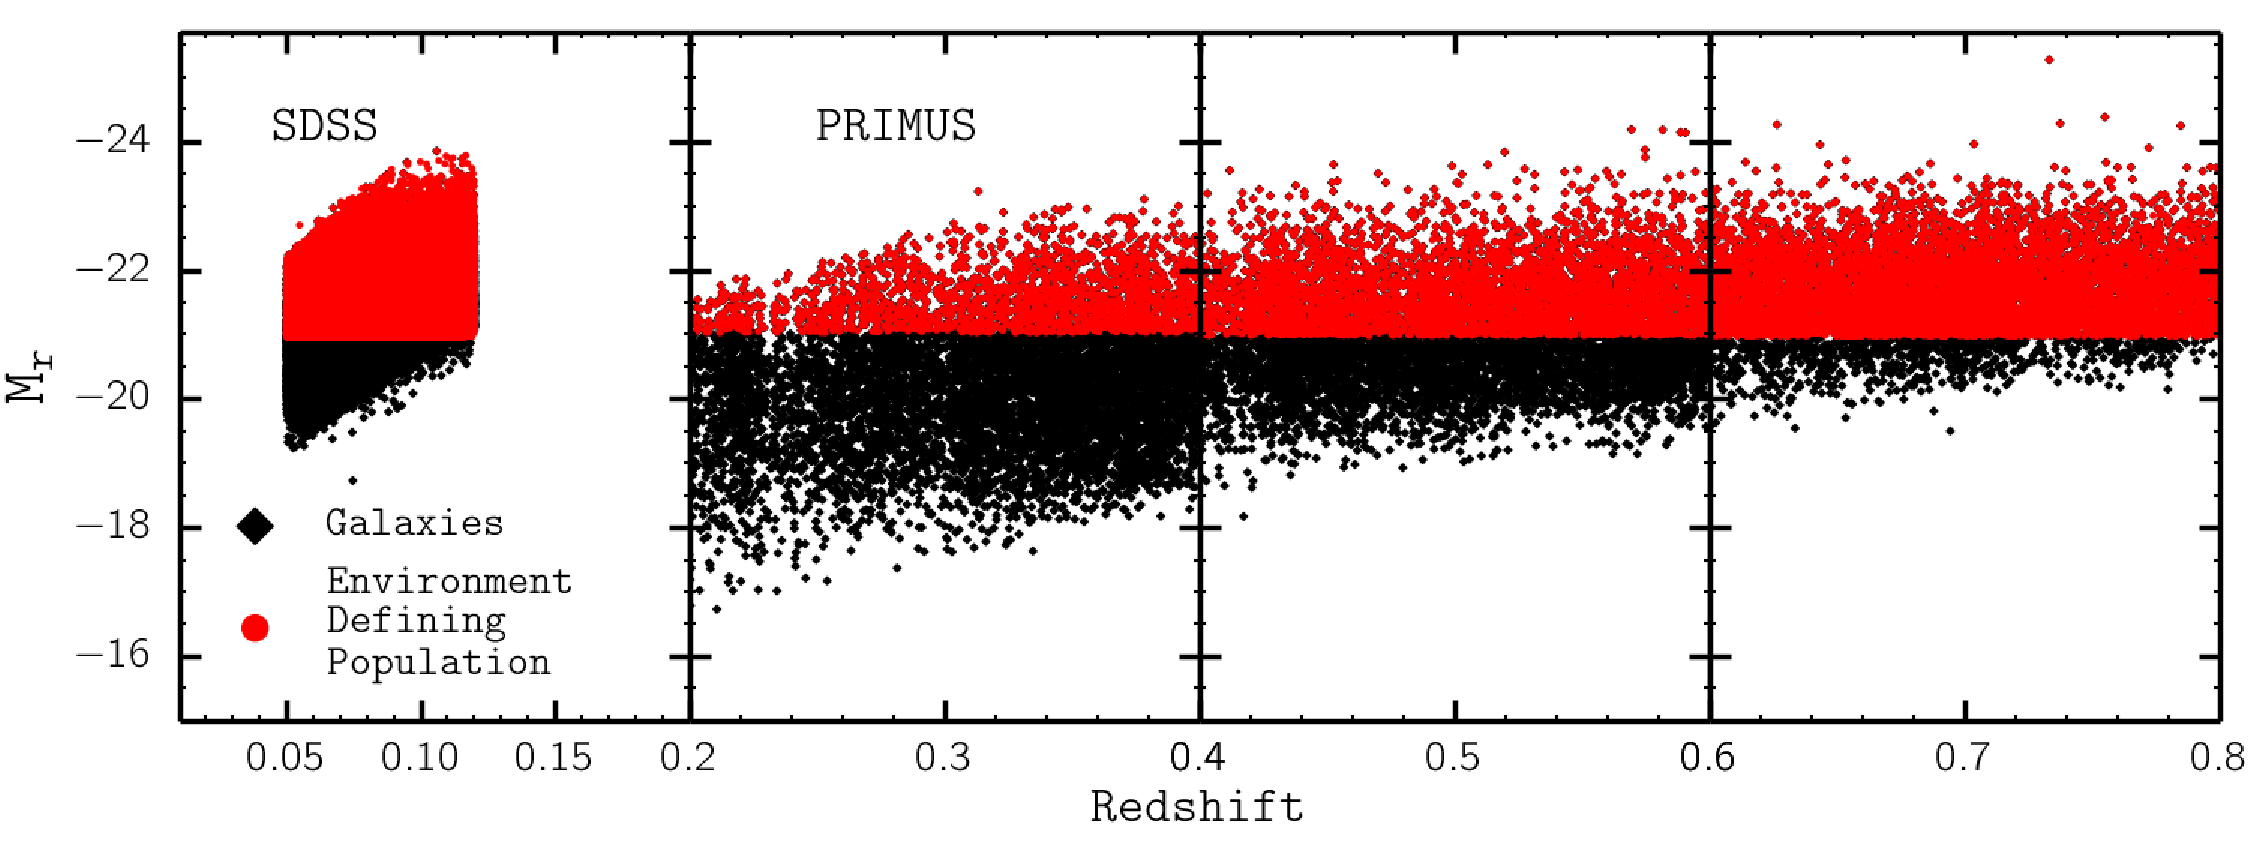
\includegraphics[width=\textwidth]{figs/qfenv/fig1.pdf}
\caption{Absolute magnitude $M_{r}$ versus redshift for our mass complete galaxy sample (black squares) with the Environment Defining Population (red circles) plotted on top. Both samples are divided into redshift bins: $z = 0.05-0.12$, $0.2-0.4$, $0.4-0.6$, and $0.6-0.8$ (panels left to right). The lowest redshift bin ($z \approx 0.05-0.12$; leftmost panel) contain our galaxy sample and EDP selected from SDSS. The rest contain galaxies and EDP selected from PRIMUS. The redshift limits for the lowest redshift bin are empirically selected based on the bright and faint limits of SDSS galaxies. Stellar mass completeness limits, described in Section \ref{sec:target}, are imposed on the galaxy population. Meanwhile, $M_{r}$ limits are applied to the EDP such that the number density in each panel are equivalent (Section \ref{sec:environment}).} \label{fig:targetEDP}
\end{center}
\end{figure*}
%%%%%%%%%%%%%%%%%%%%%%%%%%%%%%%%%%%%%%%%%%%%%%%%%%%%%%%%%%%%%%%%%%%%%%%%%%%%%%%%%%%%
% PRIMUS
%%%%%%%%%%%%%%%%%%%%%%%%%%%%%%%%%%%%%%%%%%%%%%%%%%%%%%%%%%%%%%%%%%%%%%%%%%%%%%%%%%%%
\subsection{PRIMUS} \label{sec:primus}
At intermediate redshifts we use multiwavelength imaging and
spectroscopic redshifts from PRIMUS, a faint galaxy survey with $\sim
120,000$ redshifts ($\sigma_z/(1+z) \approx 0.5 \%$) within the range
$z \approx 0-1.2$. The survey was conducted using the IMACS
spectrograph on the Magellan I Baade $6.5$-m telescope with a slitmask and low dispersion prism. For details on the PRIMUS observation methods such as survey design, targeting, and data summary, we refer readers to \cite{Coil:2011aa}. For details on redshift fitting, redshift precision and survey completeness we refer readers to \cite{Cool:2013aa}.

While the PRIMUS survey targeted seven distinct extragalactic deep fields for a total of $\sim 9 \; \mathrm{deg}^2$, we restrict our sample to five fields that have $GALEX$ and {\em Spitzer}/IRAC imaging for a total of $\sim 5.5 \; \mathrm{deg}^2$ (similar to the sample selection in \citealt{Moustakas:2013aa}). Four of these fields are a part of the {\em Spitzer} Wide-area Infrared Extragalactic Survey (SWIRE\footnote{http://swire.ipac.caltech.edu/swire/swire.html}): the European Large Area ISO Survey - South $1$ field (ELAIS-S1\footnote{http://dipastro.pd.astro.it/esis}), the Chandra Deep Field South SWIRE field (CDFS), and the XMM Large Scale Structure Survey field (XMM-LSS). The XMM-LSS consists of two separate but spatially adjacent fields: the Subaru/XMM-Newton DEEP Survey field (XMM-SXDS\footnote{http://www.naoj.org/cience/SubaruProject/SDS}) and the Canadian-France-Hawaii Telescope Legacy Survey field (XMM-CFHTLS\footnote{http://www.cfht.hawaii.edu/Science/CFHLS}). Our fifth and final field is the Cosmic Evolution Survey (COSMOS\footnote{http://cosmos.astro.caltech.edu}) field. For all of our fields we have near-UV (NUV) and far-UV (FUV) photometry from the {\em GALEX} Deep Imaging Survey (DIS; \citealt{Martin:2005aa, Morrissey:2005aa}) as well as ground-based optical and {\em Spitzer}/IRAC mid-infrared photometric catalogs. \cite{Moustakas:2013aa} provides detailed descriptions of integrated flux calculations in the photometric bands for each of our fields. Furthermore, we derive the {\em K-corrections} from the photometry using \texttt{K-correct} (v4.2; \citealt{Blanton:2007aa}). 

Finally, using the spectroscopic redshift and broad wavelength photometry we apply \texttt{iSEDfit}, a Bayesian SED modeling code, to calculate stellar masses and star formation rates (SFRs) for our sample galaxies (\citealt{Moustakas:2013aa}). \texttt{iSEDfit} uses the redshift and the observed photometry of the galaxies to determine the statistical likelihood of a large ensemble of generated model SEDs. The model SEDs are generated using Flexible Stellar Population Synthesis (FSPS) models (\citealt{Conroy:2010aa}) based on the \cite{Chabrier:2003aa} IMF, along with a time dependent dust attenuation curve of \cite{Charlot:2000aa} and other prior parameters discussed in Section 4.1 and Appendix A of \cite{Moustakas:2013aa}. For details on the effects of prior parameter choices of iSEDfit on physical properties of galaxies we refer readers to the Appendix of \cite{Moustakas:2013aa}. For the observed photometry, we use the {\em GALEX} FUV and NUV, the two shortest IRAC bands at $3.6$ and $4.5 \mu \mathrm{m}$ (the two longer-wavelength IRAC channels are excluded because \texttt{iSEDfit} does not model hot dust or polycyclic aromatic hydrocarbons emission lines), and the optical bands. 

%%%%%%%%%%%%%%%%%%%%%%%%%%%%%%%%%%%%%%%%%%%%%%%%%%%%%%%%%%%%%%%%%%%%%%%%%%%%%%%%%%%%
% SDSS-GALEX
%%%%%%%%%%%%%%%%%%%%%%%%%%%%%%%%%%%%%%%%%%%%%%%%%%%%%%%%%%%%%%%%%%%%%%%%%%%%%%%%%%%%
\subsection{SDSS-GALEX} \label{sec:sdss}
At low redshifts, we use spectroscopic redshifts and $ugriz$ photometry from the SDSS Data Release 7 (DR7; \citealt{Abazajian:2009aa}). More specifically we select galaxies from the New York University Value-Added Galaxy Catalog (hereafter VAGC) that satisfy the main sample criterion and have galaxy extinction corrected Petrosian magnitudes $14.5 < r < 17.6$ and spectroscopic redshifts within $0.01 < z < 0.2$ (\citealt{Blanton:2005aa}). We further restrict the VAGC sample to only galaxies with medium depth observations with total exposure time greater than $1 \; \mathrm{ks}$ from {\em GALEX} Release 6. This leaves $167,727$ galaxies. 

Next, we use the MAST/CasJobs\footnote{http://galex.stsci.edu/casjobs} interface and a $4''$ diameter search radius, to obtain the NUV and FUV photometry for the SDSS-{\em GALEX} galaxies. For optical photometry, we use the $ugriz$ bands from the SDSS \texttt{model} magnitudes scaled to the $r$-band \texttt{cmodel} magnitude. These photometric bands are then supplemented with integrated $JHK_s$ magnitudes from the 2MASS Extended Source Catalog (XSC; \citealt{Jarrett:2000aa}) and with photometry at $3.4$ and $4.6 \mu \mathrm{m}$ from the WISE All-Sky Data Release\footnote{http://wise2.ipac.caltech.edu/docs/release/allsky}. Further details regarding the SDSS-{\em GALEX} sample photometry can be found in Section 2.4 of \cite{Moustakas:2013aa}. As previously done on the PRIMUS data in Section \ref{sec:primus}, we use \texttt{iSEDfit} to obtain the stellar masses and star formation rates for the SDSS-{\em GALEX} sample. 

The SDSS-{\em GALEX} data discussed above is derived from the NYU-VAGC
based on SDSS Data Release 7, using the standard SDSS photometric
measurements. Several investigators have found that the background
subtraction techniques used in the standard photometric catalogs
introduce a size dependent bias in the galaxy fluxes and consequently
stellar masses (\citealt{West:2005aa, Blanton:2005ab, Lauer:2007aa, Bernardi:2007aa,
  Hyde:2009aa, West:2010aa}).

In order to quantify the effects of these photometric underestimations
in our analysis, we tried replacing our SDSS fluxes in the $ugriz$
band with $ugriz$ fluxes from the NASA-Sloan Atlas (NSA) catalog,
which incorporate the improved background subtraction presented in
\cite{Blanton:2011aa} and uses single-Seric fit fluxes rather than the
standard SDSS \texttt{cmodel} fluxes. Using the ratio of the
luminosity derived from the improved photometry over the luminosity
derived from the standard NYU-VAGC photometry, we apply a preliminary
correction to the stellar mass values obtained from \texttt{iSEDfit}
assuming a consistent mass-to-light ratio. This mass correction leads
to a significant increase in the stellar mass function for
$\mathcal{M} > 10^{11} \mathcal{M}_{\odot}$; however, the effect of
the mass correction was negligible for the quiescent fraction
evolution results. As a result, for the results presented here we use
the standard SDSS fluxes and we do not discuss the issues with
photometric measurements any further in this paper. We note that a
thorough investigation of these issues to understand their effect on
the stellar mass function requires a reanalysis of both the SDSS
photometry and the deeper photometry used for PRIMUS targeting.

%%%%%%%%%%%%%%%%%%%%%%%%%%%%%%%%%%%%%%%%%%%%%%%%%%%%%%%%%%%%%%%%%%%%%%%%%%%%%%%%%%%%
% GALAXY SAMPLE
%%%%%%%%%%%%%%%%%%%%%%%%%%%%%%%%%%%%%%%%%%%%%%%%%%%%%%%%%%%%%%%%%%%%%%%%%%%%%%%%%%%%
\begin{table*} 
  \caption{Galaxy Subsamples}
  \label{tab:subsample}
  \begin{center}
    \leavevmode
    \begin{tabular}{ccccccc} \hline \hline              
     &\multicolumn{1}{c}{$n_{\mathrm{env}}$}        & \multicolumn{2}{c}{$N_{\mathrm{gal}}$}  & \multicolumn{2}{c}{$\mathcal{M}_{\mathrm{lim}}$} & $M_{\mathrm{r}, lim}$ \\ 
    & & Quiescent & Star-Forming & Quiescent & Star-Forming &  \\ \hline 
$0.05 < z < 0.12$ & $n_{\mathrm{env}} = \lowenvthresh $ & 6533 & 7508 & $10^{10.2} \mathcal{M}_{\odot}$ & $10^{10.2} \mathcal{M}_{\odot}$ & -20.95 \\
               & $n_{\mathrm{env}} > \highenvthresh $ &14673 & 9717 &                          \\ 
                              & all          &$33553$                       & $29864$                          \\ \hline
$0.2 < z < 0.4$      &$n_{\mathrm{env}} = \lowenvthresh $           &363                    &1231 & $10^{9.8} \mathcal{M}_{\odot}$ & $10^{9.8} \mathcal{M}_{\odot}$ &-21.03 \\
               &$n_{\mathrm{env}} > \highenvthresh $            &379                    &756                           \\
               & all                & $1086$                      & $2879$                          \\ \hline
$0.4 < z < 0.6$      &$n_{\mathrm{env}} = \lowenvthresh $           &536                       &1498 & $10^{10.3} \mathcal{M}_{\odot}$ & $10^{10.3} \mathcal{M}_{\odot}$ & -20.98 \\
               &$n_{\mathrm{env}} > \highenvthresh $            &490                       &854                           \\
               & all               & $1560$                      & $3577$                          \\ \hline
$0.6 < z < 0.8$      &$n_{\mathrm{env}} = \lowenvthresh $           &567                       &1254  & $10^{10.7} \mathcal{M}_{\odot}$ & $10^{10.6} \mathcal{M}_{\odot}$ & -20.97 \\
               &$n_{\mathrm{env}} > \highenvthresh $            &498                       &671                           \\
               & all              & $1668$                      & $2964$                          \\ \hline
Total &      & \multicolumn{2}{c}{77151} & \\ \hline
  \multicolumn{4}{l}{}                                             \\       
    \end{tabular} \par
    \end{center}
%    \bigskip 
    {\bf Notes}: Number of galaxies ($N_{\mathrm{gal}}$) in the mass complete subsamples within the edges of the survey (Section \ref{sec:sample}). The subsamples are classified based on environment ($n_{\mathrm{env}}$) and star formation rate (star-forming or quiescent). The lowest redshift bin is derived from SDSS; the rest are from PRIMUS. We also list the stellar mass completeness limit, $\mathcal{M}_{\mathrm{lim}}$, for our sample along with the $r$-band absolute magnitude limits, $M_{\mathrm{r}, lim}$, for the Environment Defining Population. 
    \bigskip
\end{table*}

\subsection{Stellar Mass Complete Galaxy Sample} \label{sec:target} 
From the low redshift SDSS-{\em GALEX} and intermediate redshift
PRIMUS data we define our mass complete galaxy
sample. We begin by imposing the parent sample selection criteria from
\cite{Moustakas:2013aa}. More specifically, we take the statistically
complete {\em primary} sample from the PRIMUS data
(\citealt{Coil:2011aa}) and impose magnitude limits on optical
selection bands as specified in \cite{Moustakas:2013aa} Table 1. These
limits are in different optical selection bands and have distinct
values for the five PRIMUS target fields. We then exclude stars and
broad-line AGN to only select objects spectroscopically classified as
galaxies, with high-quality spectroscopic redshifts ($Q \geq
3$). Lastly, we impose a redshift range of $ 0.2 < z < 0.8$ for the
PRIMUS galaxy sample, where $ z > 0.2$ is selected due to limitations
from sample variance and $ z < 0.8$ is selected due to the lack of
sufficient statistics in subsamples defined below.

For the PRIMUS objects that meet the above criteria, we assign statistical weights (described in \citealt{Coil:2011aa} and \citealt{Cool:2013aa}) in order to correct for targeting incompleteness and redshift failures. The statistical weight, $w_i$, for each galaxy is given by
\begin{equation}
w_{i} = (f_{\mathrm{target}} \times f_{\mathrm{collision}} \times f_{\mathrm{success}})^{-1},
\end{equation}
as in Equation (1) in \cite{Moustakas:2013aa}. 

Since we are ultimately interested in a mass complete galaxy sample to
derive SMFs and QFs, next we impose stellar mass completeness limits
to our galaxy sample.
Stellar mass completeness limits for a magnitude-limited survey such as PRIMUS are functions of redshift, the apparent magnitude limit of the survey, and the typical stellar mass-to-light ratio of galaxies near the flux limit. We use the same procedure as \cite{Moustakas:2013aa}, which follows \cite{Pozzetti:2010aa}, to empircally determine the stellar mass completeness limits. For each of the target galaxies we compute $\mathcal{M}_{\mathrm{lim}}$ using $\log \; \mathcal{M}_{\mathrm{lim}} = \log \; \mathcal{M} + 0.4\;(m - m_{\mathrm{lim}})$, where $\mathcal{M}$ is the stellar mass of the galaxy in $\mathcal{M_{\odot}}$, $\mathcal{M}_{\mathrm{lim}}$ is the stellar mass of each galaxy if its magnitude was equal to the survey magnitude limit, $m$ is the observed apparent magnitude in the selection band, and $m_{\mathrm{lim}}$ is the magnitude limit for our five fields. We construct a cumulative distribution of $\mathcal{M}_{\mathrm{lim}}$ for the $15\%$ faintest galaxies in $\Delta z=0.04$ bins. In each of these redshift bins, we calculate the minimum stellar mass that includes $95 \%$ of the galaxies. Separately for quiescent and star-forming galaxies, we fit quadratic polynomials to the minimum stellar masses versus redshift (star-forming or quiescent classification is described in the following section). Finally, we use the polynomials to obtain the minimum stellar masses at the center of redshift bins, $0.2-0.4$, $0.4-0.6$, and $0.6-0.8$, which are then used as PRIMUS stellar mass completeness limits.

For the low redshift portion of our galaxy sample, we start by limiting the SDSS-{\em GALEX} data to objects within $0.05 < z < 0.12$, a redshift range later imposed on the volume-limited Environment Defining Population (Section \ref{sec:environment}). To account for the targeting incompleteness of the SDSS-{\em GALEX} sample, we use the statistical weight estimates provided by the NYU-VAGC catalog. Furthermore, we determine a uniform stellar mass completeness limit of $10^{10.2} \mathcal{M}_{\odot}$ above the stellar mass-to-light ratio completeness limit of the SDSS-{\em GALEX} data within the imposed redshift limits (\citealt{Blanton:2005ab, Baldry:2008aa, Moustakas:2013aa}). We then apply this mass limit in order to obtain our mass-complete galaxy sample at low redshift. 

We now have a stellar mass complete sample derived from SDSS-{\em
  GALEX} and PRIMUS data. Since our sample is derived from two
different surveys, we account for the disparity in the redshift
uncertainty. While PRIMUS provides a large number of redshifts out to
$z = 1$, due to its use of a low dispersion prism, the redshift
uncertainties are significantly larger ($\sigma_{z}/(1+z) \approx 0.5
\%$) than the uncertainties of the SDSS redshifts. In order to have
comparable environment measures throughout our redshift range, we
apply PRIMUS redshift uncertainties to our galaxy sample selected from
SDSS-{\em GALEX}. For each SDSS-{\em GALEX} galaxy, we adjust its
redshift by randomly sampling a Gaussian distribution with standard
deviation $\sigma = 0.005 (1+z_\mathrm{SDSS})$, where
$z_\mathrm{SDSS}$ is the SDSS redshift of the galaxy.

%We present the absolute magnitude ($M_{r}$) versus redshift for the galaxy sample (black squares) in Figure \ref{fig:targetEDP}. The left-most panel corresponds to the sample derived from the SDSS-{\em GALEX} data and the rest correspond to the target sample derived from the PRIMUS data divided in bins with $\Delta z \sim 0.2$. 
%%%%%%%%%%%%%%%%%%%%%%%%%%%%%%%%%%%%%%%%%%%%%%%%%%%%%%%%%%%%%%%%%%%%%%%%%%%%%%%%%%%%
% CLASSIFYING QUIESCENT AND STAR-FORMING GALAXIES
%%%%%%%%%%%%%%%%%%%%%%%%%%%%%%%%%%%%%%%%%%%%%%%%%%%%%%%%%%%%%%%%%%%%%%%%%%%%%%%%%%%%
\subsection{Classifying Quiescent and Star-Forming Galaxies} \label{sec:sfq}
We now classify our mass complete galaxy sample into quiescent or star-forming using an evolving cut based on specific star-formation rate utilized in \cite{Moustakas:2013aa} Section 3.2. This classification method uses the star-forming (SF) sequence, which is the correlation between star-formation rate (SFR) and stellar mass in star-forming galaxies observed at least until $z \sim 2$ (\citealt{Noeske:2007aa, Williams:2009aa, Karim:2011aa}). The PRIMUS sample displays a well-defined SF sequence within the redshift range of our galaxy sample. Using the power-law slope for the SF sequence from \cite{Salim:2007aa} (SFR $\propto \mathcal{M}^{0.65}$) and the minimum of the quiescent/star-forming bimodality, determined empirically, we obtain the following equation to classify the target galaxies (Equation 2 in \citealt{Moustakas:2013aa}):
\begin{equation} \label{eq:qsfclass} 
\mathrm{log}(\mathrm{SFR}_{\mathrm{min}}) = -0.49 + 0.64 \mathrm{log}(\mathcal{M} - 10) +1.07(z-0.1), 
\end{equation} 
where $\mathcal{M}$ is the stellar mass of the galaxy. If the target galaxy SFR and stellar mass lie above Equation \ref{eq:qsfclass} we classify it as star-forming; if below, as quiescent (\citealt{Moustakas:2013aa} Figure 1.).
%%%%%%%%%%%%%%%%%%%%%%%%%%%%%%%%%%%%%%%%%%%%%%%%%%%%%%%%%%%%%%%%%%%%%%%%%%%%%%%%%%%%
% GALAXY ENVIRONMENT
%%%%%%%%%%%%%%%%%%%%%%%%%%%%%%%%%%%%%%%%%%%%%%%%%%%%%%%%%%%%%%%%%%%%%%%%%%%%%%%%%%%%
\begin{figure}
\begin{center}
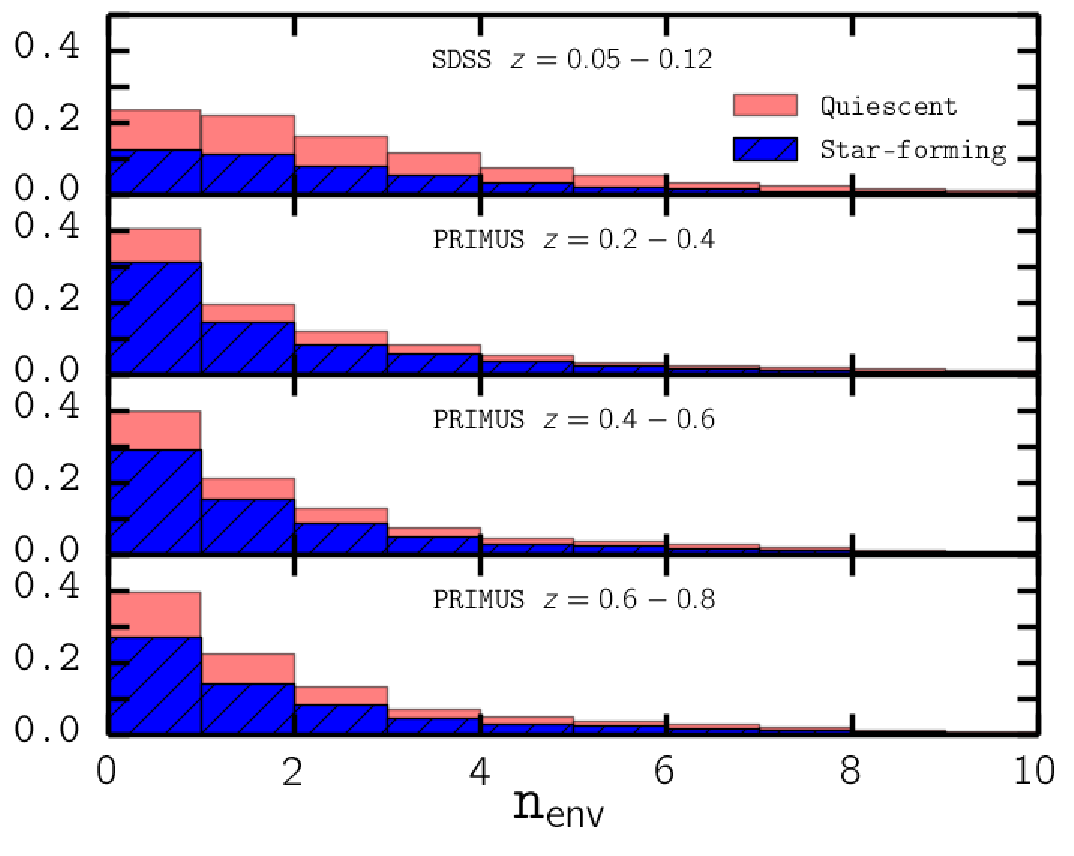
\includegraphics[width=\textwidth]{figs/qfenv/fig2.pdf}
\caption{Normalized distribution of environment measurements ($n_{\mathrm{env}}$) for our mass complete galaxy sample within the survey edges. A fixed cylindrical aperture of $R_{\mathrm{ap}} =\apradius\;\mathrm{Mpc}$ and $H_{\mathrm{ap}} = \apheight\; \mathrm{Mpc}$ is used to measure environment. The star-forming galaxies contribution to the distribution is colored in blue and diagonally patterned. The contribution from quiescent galaxies is colored in red. Galaxies with $n_{\mathrm{env}} = 0.0$ are in low density environments and galaxies with $n_{\mathrm{env}} > 3.0$ are in high density environment. We note that the significant difference among the SDSS distribution and the PRIMUS distributions above is due to the different stellar mass completeness limits imposed on each redshift bin of our galaxy sample.}      \label{fig:envcount}
 %\caption{Normalized distribution of environment measurements ($n_{\mathrm{env}}$) for our mass complete galaxy sample within the edges. The star-forming galaxies contribution to the distribution is colored blue and diagonally patterned. The contribution from quiescent galaxies is colored in red. Each redshift panel is divided into three sections by the environment classification cutoffs (black veritcal lines): low density environment $n_{\mathrm{env}} < 0.5$ and high density environment $n_{\mathrm{env}} > 3.0$. The percentages of the redshift bin contained in the environment classifications are presented above the distribution. For example at $0.2 < z < 0.4$, $\apheight.0 \%$ of galaxies in the redshift bin are in low density environments while $35.0\%$ of galaxies in the redshift bin are in high density environments. We note that the significant difference between the SDSS distribution and the PRIMUS distribution above is due to the difference in stellar mass completeness limit imposed in our galaxy sample.}      \label{fig:envcount}
\end{center}
\end{figure}

\subsection{Galaxy Environment} \label{sec:environment}
We define the environment of a galaxy as the number of neighboring Environment Defining Population galaxies (defined below) within a fixed aperture centered around it. We use fixed aperture measurements in order to quantify galaxy environment with an aperture sufficiently large to encompass massive halos (\citealt{Muldrew:2012aa, Skibba:2013aa}).
%We use a fixed aperture measurement of environment in order to probe environment on the halo scale, as \cite{Muldrew:2012aa} finds in their comparison of different environment definition using simulations.

For our aperture, we use a cylinder of dimensions: $R_{\mathrm{ap}} = \apradius\;
\mathrm{Mpc}$ and $H_{\mathrm{ap}} = \apheight\; \mathrm{Mpc}$. We note that $H_\mathrm{ap}$ is the full height of the cylinder and $R_\mathrm{ap}$ 
and $H_\mathrm{ap}$ are comoving distances. We use a
cylindrical aperture to account for the PRIMUS redshift
errors and redshift space distortions (i.e. ``Finger of God"
effect). As \cite{Cooper:2005aa} and \cite{Gallazzi:2009aa} find, 
$\pm 1000 \; \mathrm{km} \;\mathrm{s^{-1}}$ optimally reduces the effects of redshift space
distortions. The PRIMUS redshift uncertainty at $z \sim 0.7$
corresponds to $\sigma_z < 0.01$, so our choice of $\apheight\;
\mathrm{Mpc}$ for the aperture height accounts for both of these effects. Our choice of
cylinder radius was motivated by scale dependence analyses in the
literature (\citealt{Blanton:2006ab, Wilman:2010aa, Muldrew:2012aa}),
which suggest that galactic properties such as color and quiescent
fractions are most strongly dependent on scales $< 2$ Mpc, around the
host dark matter halo sizes.

% Not sure we need to note this detail; the anticorrelation is small.
%\cite{Wilman:2010aa}, which uses environment defined by annuli of
%different radii, find positive correlation for quiescent fraction and
%color on scales $< 1 \; \mathrm{Mpc}$ and anti-correlation on scales $> 3
%\; \mathrm{Mpc}$. Our choice of $2 \mathrm{Mpc}/h$ provides sufficient sample
%size of galaxies in dense environments, for robust statistics, while
%tracing galactic properties within the halo scale.

Before we measure the environment for our galaxy sample, we first
construct a volume limited Environment Defining Population (EDP) with
absolute magnitude cut-offs ($M_{r}$) in redshift bins with $\Delta z
\sim 0.2$. The $M_{r}$ cut-offs for the EDP are selected such that the
cumulative number density over $M_{r}$ for all redshift bins are
equal.  We make this choice in order to construct an EDP that contains
similar galaxy populations through the redshift range (i.e. accounts
for the progenitor bias). In their analysis of this method,
\cite{Behroozi:2013aa} and \cite{Leja:2013aa} find that although it
does not precisely account for the scatter in mass accretion or
galaxy-galaxy mergers, it provides a reasonable means to compare
galaxy populations over a wide range of cosmic time.

In constructing the PRIMUS EDP we use the same PRIMUS data used to select our galaxy sample (described in Section \ref{sec:target}). We again restrict the PRIMUS galaxies to $0.2 < z < 0.8$ and divide them into bins of $\Delta z = 0.2$. Before we consider the cumulative number densities in the redshift bins, we first determine the $M_r$ limit for the highest redshift bin ($z = 0.6-0.8$) by examining the $M_{r}$ distribution with bin size $\Delta M_{r} = 0.25$ and select $M_{r,\mathrm{lim}}$ near the peak of the distribution where bins with $M_{r} > M_{r,\mathrm{lim}}$ have fewer galaxies than the bin at $M_{r, \mathrm{lim}}$. We conservatively choose $M_{r, \mathrm{lim}}(0.6 < z < 0.8)$ to be $M_{r} = -20.97$. Then for the lower redshift bins, we impose absolute magnitude limits ($M_{r,\mathrm{lim}}$) such that the cumulative number density, calculated with the galaxy statistical weights, of the bin ordered by $M_{r}$ is equal to the cumulative number density of the highest redshift bin with $M_{r, \mathrm{lim}}(0.6 < z < 0.8) = -20.97$. 

For the SDSS EDP, we do not use the SDSS-{\em GALEX} parent data,
which is limited to the combined angular selection window of the
VAGC and {\em GALEX} (Section \ref{sec:sdss}). Instead, since FUV, NUV
values are not necessary for the EDP, we extend the parent data of the
SDSS EDP to the entire NYU-VAGC, including galaxies outside of the
{\em GALEX} window function. Furthermore, we impose a redshift range
of $0.05-0.12$ on the SDSS EDP. This redshift range was determined to
account for the lack of faint galaxies at $z \sim 0.2$ and the lack of
bright galaxies at $z \sim 0.01$ in the VAGC. As with the PRIMUS
redshift bins, we determine the SDSS EDP $M_{r, \mathrm{lim}}$ by matching
the cumulative number density of the highest redshift bin. For
redshift bins $z = 0.05-0.12$, $0.2-0.4$, $0.4-0.6$, $0.6-0.8$ we get
$M_{r,\mathrm{lim}} = -20.95$, $-21.03$, $-20.98$ and $-20.97$,
respectively. These absolute magnitude limits are illustrated in
Figure \ref{fig:targetEDP}, where we present the absolute magnitude ($M_{r}$) versus redshift for the galaxy sample (black squares) ad the EDP (red circles). 
The left-most panel corresponds to the samples derived from the SDSS-{\em GALEX} data while the rest correspond to samples derived from the PRIMUS data divided in bins with $\Delta z \sim 0.2$. 
Figure \ref{fig:targetEDP} shows clear $M_r$ cutoffs in the
$M_{r}$ distribution versus redshift for the EDP on top
of our galaxy sample.

For our SDSS-{\em GALEX} galaxy sample, in Section \ref{sec:target}, we apply PRIMUS redshift errors in order to establish a consistent measurement of environment throughout our redshift range. We appropriately apply equivalent redshift adjustments for the SDSS EDP. For the SDSS EDP galaxies that are also contained within the SDSS-{\em GALEX} sample, we adjust the redshift by an identical amount. For the rest, we apply the same redshift adjustment procedure described in Section \ref{sec:target} in order to obtain PRIMUS level redshift uncertainties. 

Finally, we measure the environment for each galaxy in our galaxy
sample by counting the number of EDP galaxies, $n_{\mathrm{env}}$, with RA,
Dec, and $z$ within our cylindrical aperture centered around
it. $n_{\mathrm{env}}$ accounts for the statistical weights of the EDP
galaxies. 
For our galaxy sample, the expected $n_{\mathrm{env}}$ given the uniform number density in 
each of our EDP redshift bin and volume of our cylindrical aperture is $\langle n_{\mathrm{env}} \rangle = 1.3$. 
Once we obtain environment measurements for all the galaxies
in our galaxy sample, we classify galaxies with $n_{\mathrm{env}} = 0.0$
to be in ``low" environment densities and galaxies with $n_{\mathrm{env}} > 3$
to be in ``high" environment densities. The high environment cutoff was
selected in order to reduce contamination from galaxies in low
environment densities while maintaining sufficient statistics. In
Section \ref{sec:env_qf_evol} we will also explore higher density
cutoffs for $n_{\mathrm{env}}$.

The analysis we describe below uses a fixed cylindrical aperture with
dimensions $R_{\mathrm{ap}} = \apradius \; \mathrm{Mpc}$ and $H_{\mathrm{ap}} = \apheight
\;\mathrm{Mpc}$ to measure environment. The same analysis was
extended for varying aperture dimensions $R_{\mathrm{ap}} = 1.5, \: \apradius, \:3.0 \:
\mathrm{Mpc}$ and $H_{\mathrm{ap}} = \apheight, \; 70 \;\mathrm{Mpc}$ with adjusted environment classifications. 
The results obtained from using different apertures and
environment classifications are qualitatively consistent with the results presented below.  

%%%%%%%%%%%%%%%%%%%%%%%%%%%%%%%%%%%%%%%%%%%%%%%%%%%%%%%%%%%%%%%%%%%%%%%%%%%%%%%%%%%%
% EDGE EFFECTS
%%%%%%%%%%%%%%%%%%%%%%%%%%%%%%%%%%%%%%%%%%%%%%%%%%%%%%%%%%%%%%%%%%%%%%%%%%%%%%%%%%%%
\subsection{Edge Effects} \label{sec:edgeeffect}
One of the challenges in obtaining accurate galaxy environments using a fixed aperture method is accounting for the edges of the survey. For galaxies located near the edge of the survey, part of the fixed aperture encompassing it will lie outside the survey regions. In this scenario, $n_{env}$ only reflects the fraction of the environment within the survey geometry.

To account for these edge effects, we use a Monte Carlo method to impose edge cutoffs on our galaxy sample. First, using \texttt{ransack} from \cite{Swanson:2008aa}, we construct a random sample of  $N_{\mathrm{ransack}} = 1,000,000$ points with RA and Dec randomly selected within the window function of the EDP (SDSS EDP and PRIMUS EDP separately). We then compute the angular separation, $\theta_{i, \mathrm{ap}}$ that corresponds to $R_{\mathrm{ap}}$ (Section \ref{sec:environment}) at the redshift of each sample galaxy $i$. For each sample galaxy we count the number of \texttt{ransack} points within $\theta_{i, \mathrm{ap}}$ of the galaxy: $n_{i,\mathrm{ransack}}$. Afterwards, we compare $n_{i,\mathrm{ransack}}$ to the expected value computed from the angular area of the environment defining aperture and the EDP window function: 
\begin{equation} \label{eq:ransack}
\langle n_{\mathrm{ransack}}\rangle_{i} = \frac{N_{\mathrm{ransack}}}{A_{\mathrm{EDP}}}\times {\pi \theta_{i, \mathrm{ap}}^2} \times f_{\mathrm{thresh}}. 
\end{equation} 
$A_{\mathrm{EDP}}$ is the total angular area of the EDP window function and $f_{\mathrm{thresh}}$ is the fractional threshold for the edge effect cut-off. For $R_{\mathrm{ap}}= \apradius \;\mathrm{Mpc}$, we use $f_{\mathrm{thresh}} = 0.75$. If $n_{i, \mathrm{ransack}} > \langle n_{\mathrm{ransack}} \rangle_i$ then galaxy $i$ remains in our sample; otherwise, it is discarded. Once the edge effect cuts are applied, we are left with the final galaxy sample. For our SDSS-{\em GALEX} galaxy sample, $\sim 12 \%$ of galaxies are removed from the edge effect cuts. For our PRIMUS galaxy sample, $\sim 40 \%$ of galaxies are removed from the edge effect cuts. 

In Figure \ref{fig:envcount} we present the distribution of environment measurements ($n_{\mathrm{env}}$) for our final galaxy sample in redshift bins: $z = 0.05 - 0.12$, $0.2 - 0.4$, $0.4-0.6$, and $0.6-0.8$. The quiescent galaxy contributions are colored in red while the star-forming galaxy contributions are colored in blue and patterned. We classify galaxies with $n_{\mathrm{env}} = 0.0$ to be in low density environments and galaxies with $n_{\mathrm{env}} > 3.0$ to be in high density environments. 

Although we imposed PRIMUS redshift errors on our SDSS galaxies to consistently measure environment throughout our entire sample, we note a significant discrepancy between the $n_{\mathrm{env}}$ distributions of the SDSS and PRIMUS samples. For example, in each of the PRIMUS redshift bins, $\sim 40 \%$ of galaxies in the redshift bin are in low density environments and roughly $30 \%$ are in high density environments. In contrast, in the SDSS redshift bin, $\sim 20 \%$ of galaxies in the redshift bin are in low density environments and $\sim 35 \%$ are in high density environments. We remind the reader that this is mainly due to the varying stellar mass-completeness limits imposed on our galaxy sample for each redshift bins and does not affect our results. 
\begin{figure*}
\begin{center}
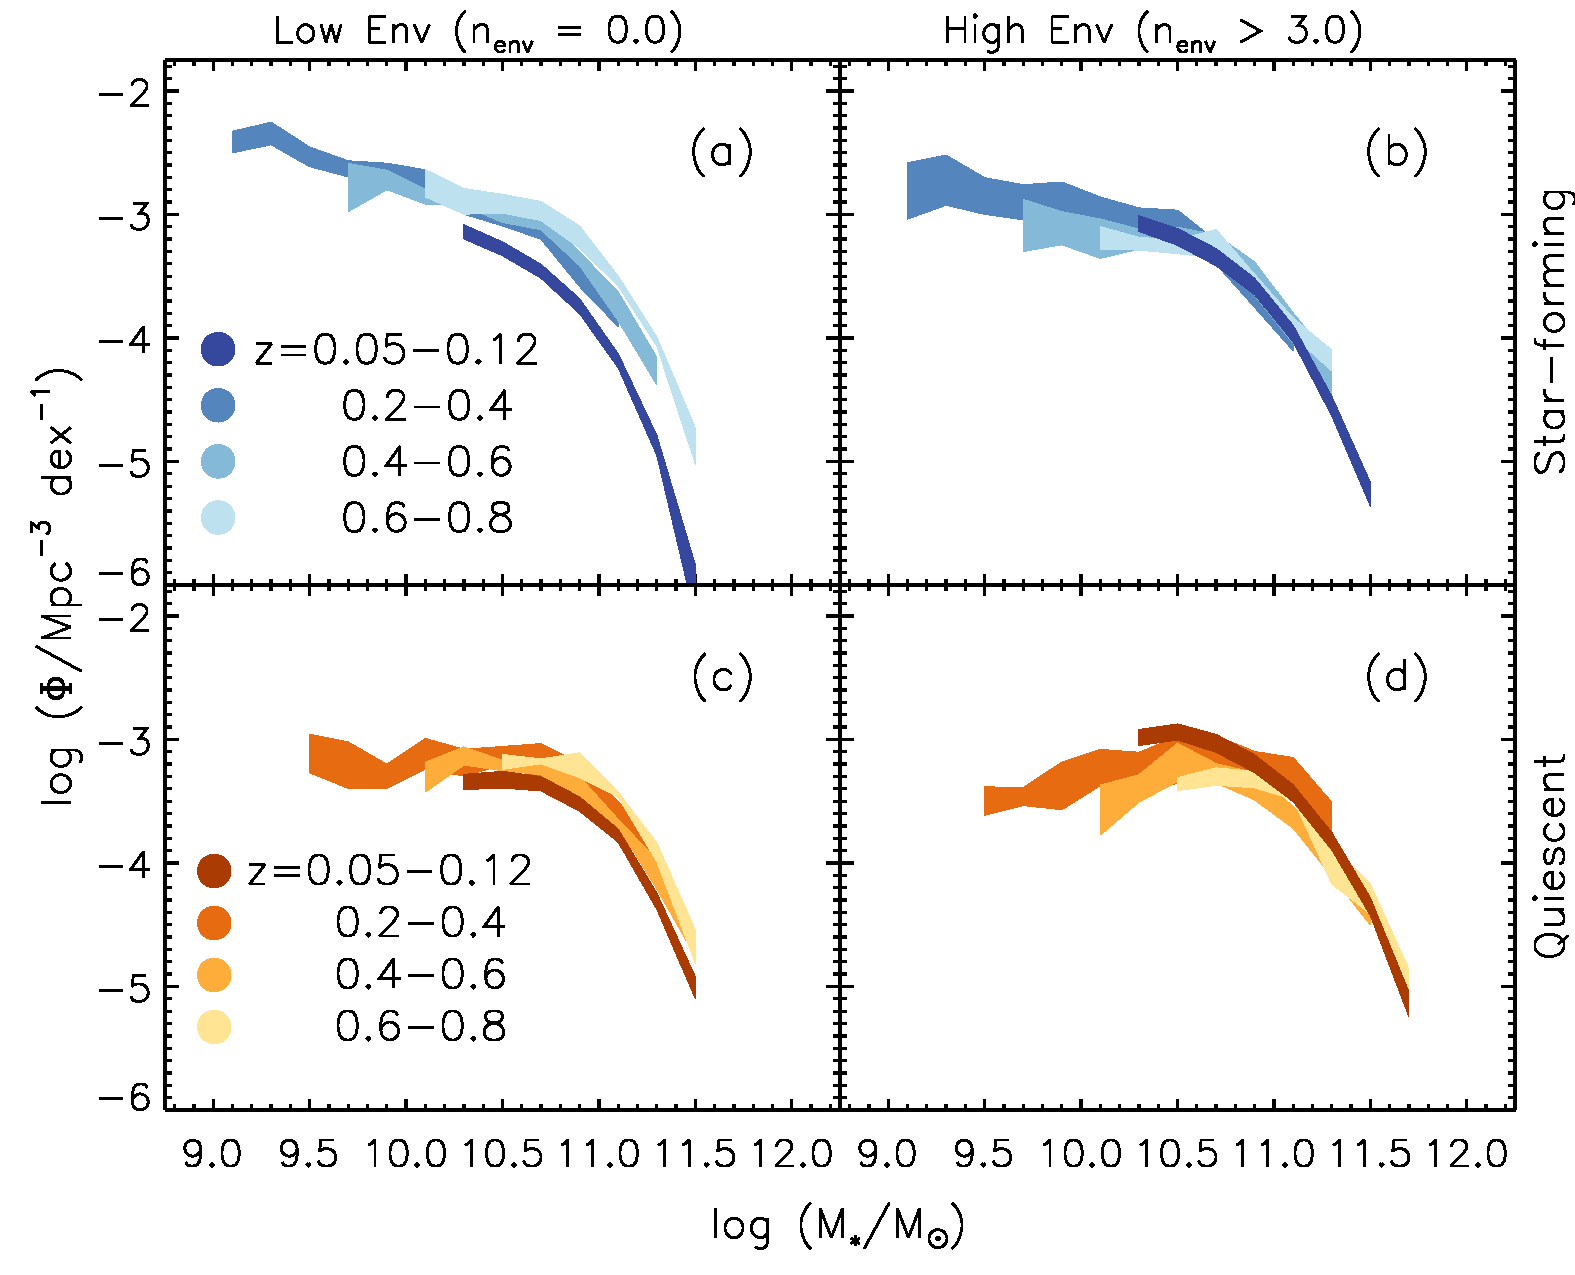
\includegraphics[width=\textwidth]{figs/qfenv/fig3.pdf}
     \caption{Evolution of stellar mass functions of star-forming (top) and quiescent (bottom) galaxies in 
low (left) and high (right) density environments throughout the redshift range
$z=0$--$0.8$. The environment of each galaxy  
was calculated using a cylindrical aperture size of $R=\apradius \: \mathrm{Mpc}$ and $H=\apheight \: \mathrm{Mpc}$ and classified as low environment when $n_{\mathrm{env}} = 0.0$ and as high environment when $n_{\mathrm{env}} > 3.0$. The SMFs use mass bins of 
width $\Delta \mathrm{log}(\mathcal{M}/\mathcal{M}_{\odot})=0.2$. In each panel we use shades of blue 
(star-forming) and orange (quiescent) to represent the SMF at different redshift, higher redshifts being
progressively lighter.}      \label{fig:smf}
\end{center}
\end{figure*}
%%%%%%%%%%%%%%%%%%%%%%%%%%%%%%%%%%%%%%%%%%%%%%%%%%%%%%%%%%%%%%%%%%%%%%%%%%%%%%%%%%%%
% STELLAR MASS FUNCTION
%%%%%%%%%%%%%%%%%%%%%%%%%%%%%%%%%%%%%%%%%%%%%%%%%%%%%%%%%%%%%%%%%%%%%%%%%%%%%%%%%%%%
\section{Results: Stellar Mass Function} \label{sec:smf}
Our galaxy sample has so far been classified into quiescent or
star-forming and low or high density environments. We further divide
these subsamples into redshift bins: $0.05-0.12$, $0.2-0.4$,
$0.4-0.6$, and $0.6-0.8$ for a total of 16 subsamples. In Section \ref{sec:smfcalc}, we calculate the SMF for each of these subsamples. Then we examine the evolution of active and quiescent subsample SMFs in different environments in Section \ref{sec:smfevol}.  
%%%%%%%%%%%%%%%%%%%%%%%%%%%%%%%%%%%%%%%%%%%%%%%%%%%%%%%%%%%%%%%%%%%%%%%%%%%%%%%%%%%%
% STELLAR MASS FUNCTION CALCULATIONS
%%%%%%%%%%%%%%%%%%%%%%%%%%%%%%%%%%%%%%%%%%%%%%%%%%%%%%%%%%%%%%%%%%%%%%%%%%%%%%%%%%%%
\subsection{Stellar Mass Function Calculations} \label{sec:smfcalc} 
To calculate the SMFs we employ a non-parametric $1/{V_{\mathrm{max}}}$ estimator commonly used for galaxy luminosity functions and stellar mass functions in order to account for Malmquist bias, as done in \cite{Moustakas:2013aa} and discussed in the review \cite{Johnston:2011aa}. The differential SMF is given by the following equation:
\begin{equation} \label{eq:phi}
\Phi(\mathrm{log}\: \mathcal{M}) \Delta(\mathrm{log} \:\mathcal{M}) = \sum\limits_{i=1}^{N} \frac{w_i}{V_{\mathrm{max,avail},i}}. 
\end{equation}
$w_i$ is the statistical weight of galaxy $i$ and $\Phi(\mathrm{log}\:
\mathcal{M}) \Delta(\mathrm{log}\: \mathcal{M})$ is the number of galaxies
($N$) per unit volume within the stellar mass range $[\mathrm{log}
  \mathcal{M},\: \mathrm{log} \mathcal{M}+\Delta(\mathrm{log}\mathcal{M})]$. The equation above is the same as Equation 3 in \cite{Moustakas:2013aa} except that we use $V_{\mathrm{max,avail}}$ instead than $V_{\mathrm{max}}$, to account for the edge effects of the survey discussed in Section \ref{sec:edgeeffect}. 

$V_{\mathrm{max},i}$ is the maximum cosmological volume where it is
possible to observe galaxy $i$ given the apparent magnitude limits of
the survey. However in Section \ref{sec:edgeeffect} we remove galaxies
that lie on the survey edges from our sample. In doing so, we reduce the
maximum cosmological volume where a galaxy can be observed, thereby
reducing the fraction of $V_{\mathrm{max},i}$ that is actually available
in the sample. We introduce the term $V_{\mathrm{max,avail},i}$ to express
the maximum volume accounting for the survey edge effects.

To calculate $V_{\mathrm{max,avail},i}$, we use a similar Monte Carlo
method as the edge effect cutoffs in Section
\ref{sec:edgeeffect}. First, we generate a sample of points with
random RA, Dec within the window function of our galaxy sample
(SDSS-{\em GALEX} window function and the five PRIMUS fields) and
random $z$ within the redshift range. These points are not to be
confused with the \texttt{ransack} sample in Section
\ref{sec:edgeeffect}. We apply the edge effect cuts on these random
points as we did for our galaxy sample using the same method as in
Section \ref{sec:edgeeffect}. Within redshift bins of $\Delta z \sim
0.01$, we calculate the fraction of the random points that remain in
the bin after the edge effect cuts over the total number of random
points in the bin: $f_{\mathrm{edge}}$. We then apply this factor to
compute $V_{\mathrm{max,avail}} = V_{\mathrm{max}} \times f_{\mathrm{edge}}$. The
$V_{\mathrm{max}}$ values in the equation above are computed following the
method described in \cite{Moustakas:2013aa} Section 4.2 with the same
redshift-dependent $K$-correction from the observed SED and luminosity
evolution model.

To calculate the uncertainty of the SMFs from the sample variance, we use a standard jackknife technique (following \citealt{Moustakas:2013aa}). For the PRIMUS galaxies, we calculate SMFs after excluding one of the five target fields at a time. For the SDSS target galaxies we divide the field into a 12 $\times$ 9 rectangular RA and Dec grid and calculate the SMFs after excluding one grid at a time. From the calculated SMFs we calculate the uncertainty: 
\begin{equation}
\sigma^j = \sqrt{\frac{N-1}{N} \sum\limits_{k=1}^{M} (\Phi^j_k - \langle \Phi^j \rangle)^2}
\end{equation} 
$N$ in this equation is the number of jackknife SMFs in the stellar mass bin. $\langle \Phi^j \rangle$ is the mean number density of galaxies in each stellar mass bin for all of the jackknife $\Phi^j$s. 

\subsection{Evolution of the Stellar Mass Function in Different Environments} \label{sec:smfevol}
In Figure \ref{fig:smf}, we present the SMFs of the quiescent/star-forming (orange/blue, bottom/top panels) and high/low density environment (left/right panels) subsamples. The redshift evolution of the SMFs in each of these panels are indicated by a darker shade for lower redshift bins. The width of the SMFs represent the sample variance uncertainties derived in Section \ref{sec:smfcalc}.

While a detailed comparison of the SMFs in each panel for different
epochs is complicated by the different stellar mass completeness limits, we present some notable trends in each panel. In panel (a), star-forming galaxies in low density environments, we find a significant decrease in the high mass end of the SMF ($\mathcal{M} > 10^{10.75} \mathcal{M}_{\odot}$) over cosmic time. Meanwhile at lower masses ($\mathcal{M} < 10^{10.5} \mathcal{M}_{\odot}$), we observe no noticeable trend in the SMF. In panel (b), star-forming galaxies in high density environments, we do not observe any clear trends above the knee of the SMF ($\mathcal{M} \sim 10^{10.7} \mathcal{M}_{\odot}$) but an increase in SMF below the knee. For the quiescent population in low density environment, panel (c), we observe a potential decrease at higher masses ($\mathcal{M} > 10^{10.7} \mathcal{M}_{\odot}$). Lastly for the quiescent population in high density environments, panel (d), we find significant increase in $\Phi$ for lower masses but little trend at higher masses. 
%do not notice any clear SMF evolution throughout the mass range. 

%In comparison to results from DEEP2 (\citealt{bundy06a}) and zCOSMOS (\citealt{Bolzonella:2010aa}), some of the noted trends are not immediately evident. However, this is mostly due to the conflicting mass limits proposed in each study. In addition, only part of the redshift range probed by \cite{bundy06a} overlap with our results. Overall, we find that the trends we note in the SMF evolution above are in good agreement with \cite{bundy06a} and \cite{Bolzonella:2010aa}. 

\begin{figure*}
\begin{center}
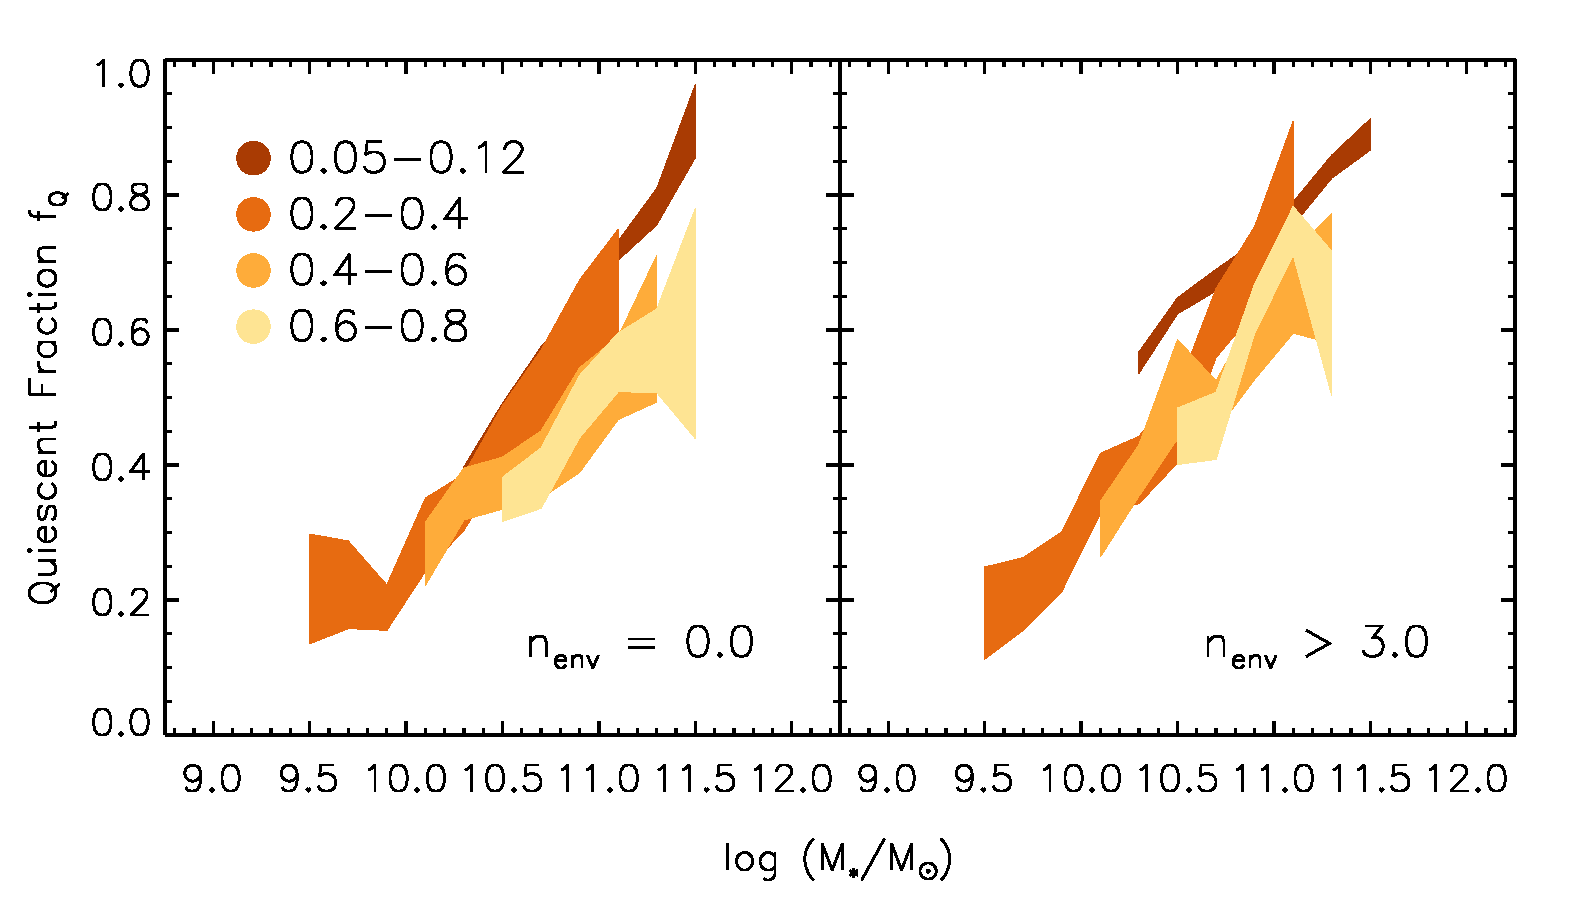
\includegraphics[width=\textwidth]{figs/qfenv/fig4.pdf}
\caption{Evolution of the quiescent fraction $f_{\mathrm{Q}}$ for
  galaxies in low (left) and high (right) density
  environments for $z < 0.8$. $f_{\mathrm{Q}}$s were calculated
  using the SMFs in Figure \ref{fig:smf}, as described in Section \ref{sec:qfevol}. Darker shading indicates lower redshift and the width represents the standard jackknife uncertainty.}         
\label{fig:qf}
\end{center}
\end{figure*}

Observing the evolutionary trends in SMF for each of these
sub-populations provides a narrative of the different galaxy
evolutionary tracks involving environment and the end of star
formation. For example, the decrease in the massive star-forming
galaxies in low density environments over cosmic time can be
attributed to the transition of those galaxies to any of the other
panels. The star-forming galaxies in low density environments that
have ended star formation over time are possibly responsible
for the increase of the quiescent, low density environment SMF over
time. The star-forming galaxies that fall into higher density
environments explain the increase in the star-forming high density
environment SMF below the knee. Finally, star-forming galaxies in high
density environments that have ended their star-formation,
quiescent galaxies that have transitioned from low to high density
environments, and star-forming galaxies in low density environments
that end their star-formation while infalling to high density
environments all contribute to the overall increase of the high
environment quiescent SMF.

In addition to the evolution over cosmic time, we observe noticeable
trends when we compare the SMFs for star-forming and quiescent
galaxies between the two environments. Comparison of the SMFs in low
versus high density environments reveal a noticeable relation between
mass and density, with SMFs in high density environments having more
massive galaxies, especially evident in our lowest redshift bin. 
We further confirm this trend when we compare the
%massive galaxies. We further confirm this trend w hen we compare the
median mass between the two environments to find that the median mass
for galaxies in high density environments is significantly greater
than in low density environments. The relationship between mass and
environment observed in our SMFs reflects the well-established
mass-density relation and observed mass segregation with environment
in the literature (\citealt{norberg02a, zehavi02a, Blanton:2005ab,
  bundy06a, Scodeggio:2009aa, Bolzonella:2010aa}).

While our mass complete subsample coupled with robust environment
measurements allows us to compare SMF evolution for each of our
subsamples out to $z=0.8$, we caution readers regarding the
photometric biases affecting the SDSS imaging (and perhaps the other
imaging sources) and reserve detailed analysis of the SMFs for 
future investigation.

%%%%%%%%%%%%%%%%%%%%%%%%%%%%%%%%%%%%%%%%%%%%%%%%%%%%%%%%%%%%%%%%%%%%%%%%%%%%%%%%%%%%
% QUIESCENT FRACTION
%%%%%%%%%%%%%%%%%%%%%%%%%%%%%%%%%%%%%%%%%%%%%%%%%%%%%%%%%%%%%%%%%%%%%%%%%%%%%%%%%%%%
\section{Results: Quiescent Fraction} \label{sec:qf_const}
The SMFs calculated in the previous section illustrate the stellar
mass distribution of our galaxy population and its evolution over
cosmic time. In this section, using the SMFs of our subsamples, we
compare the quiescent and the star-forming populations by calculating
the fraction of galaxies that have ended their star-formation, the quiescent fraction. 

While the fractional relation of the star-forming and quiescent
populations has been investigated in the past, with limited
statistics, disentangling the environmental effects from underlying
correlations among observable galaxy properties such as the color-mass
or mass-density relations (\citealt{Cooper:2010aa}) remains a 
challenge. With the better statistics available from SDSS and
PRIMUS, we evaluate the quiescent fraction in bins of stellar mass,
redshift, and environment in Section \ref{sec:qfevol}. By analyzing
the quiescent fraction with respect to these properties, in Section
\ref{sec:env_qf_evol} we explicitly compare the quiescent fraction
evolution in low and high density environments. Our comparison reveal
the subtle environmental effects on the quiescent fraction
evolution. Furthermore, by quantifying this environmental effect, we
are able constrain the role of environmental effects on how galaxies
end their star formation.
%With the sufficient statistics available from SDSS and PRIMUS, we evaluate the quiescent fraction in bins of stellar mass and redshift for low and high density environments (Section \ref{sec:qfevol}). More specifically, by analyzing the quiescent fraction with respect to mass, redshift, and environment we are able to compare the quiescent fraction evolution in low and high density environments. Through this comparison, in Section \ref{sec:env_qf_evol}, we reveal the subtle environmental effects in quenching star formation that are often obscured by the underlying correlations among galactic properties such as color-mass and mass-density relations (\citealt{Cooper:2010aa}). Furthermore by quantifying the environmental effects of star-formation quenching, we are able to provide constraints on the various proposed environmental quenching mechanisms, such as strangulation and ram-pressure stripping (\citealt{McCarthy:2008aa}).
%%%%%%%%%%%%%%%%%%%%%%%%%%%%%%%%%%%%%%%%%%%%%%%%%%%%%%%%%%%%%%%%%%%%%%%%%%%%%%%%%%%%
% EVOLUTION OF THE QUIESCENT FRACTION
%%%%%%%%%%%%%%%%%%%%%%%%%%%%%%%%%%%%%%%%%%%%%%%%%%%%%%%%%%%%%%%%%%%%%%%%%%%%%%%%%%%%
\subsection{Evolution of the Quiescent Fraction} \label{sec:qfevol}
From the SMF number densities ($\Phi$) computed in the previous section, the quiescent fraction is computed as follows, 
\begin{equation}
f_{\mathrm{Q}} ( \mathcal{M}_{*}, z)= \frac{\Phi_{Q}}{\Phi_{SF}+\Phi_{Q}}.
\end{equation}
$\Phi_{Q}$ and $\Phi_{SF}$ are the total number of galaxies per unit
volume in stellar mass bin of $\Delta(\mathrm{log} \: \mathcal{M}) = 0.20
\: \mathrm{dex}$ for the quiescent and star-forming subsamples,
respectively (Equation \ref{eq:phi}). We compute $f_{\mathrm{Q}}$ for high
and low density environments for all redshift bins as plotted in
Figure \ref{fig:qf}, which shows the evolution of $f_{\mathrm{Q}}$ for
high (right panel) and low (left panel) density environments. As in
Figure \ref{fig:smf}, the evolution of the quiescent fraction over
cosmic time is represented in the shading (darker with lower redshift)
and the uncertainty is represented by the width. For the uncertainty
in the quiescent fraction, we use the standard jackknife technique,
following the same steps as for the SMF uncertainty in Section \ref{sec:smfcalc}. 

Most noticeably in Figure \ref{fig:qf}, we find $f_{\mathrm{Q}}$ increases
monotonically as a function of mass at all redshifts and
environments. In other words, for galaxies in any environment since $ z \sim 0.8$, galaxies with higher
masses are more likely to have ceased their star-formation. With the roughly linear correlation between galaxy SFR to galaxy color and morphology, we find that this trend reflects the well established color-mass and morphology-mass relations: more massive galaxies are more likely to be red or early-type (\citealt{blanton09a}). 

Focusing on the redshift evolution of $f_{\mathrm{Q}}$, we find that for
both environments $f_{\mathrm{Q}}$ increases as redshift decreases. For
high density environments, this is analogous to the Butcher-Oemler
Effect (\citealt{Butcher:1984aa}), which states that galaxy
populations in groups or clusters have higher $f_{\mathrm{blue}}$ 
(lower $f_{\mathrm{Q}}$) at higher redshift. This evolution occurs with
roughly the same amplitude in low environments as well.

In addition, when we compare the stellar masses at which $f_{\mathrm{Q}} =
0.5$ for each subsample, the so-called $\mathcal{M}_{50-50}$, we find
that this quantity decreases over cosmic time. This corresponds to the
well-known mass-downsizing pattern found by previous investigators
(e.g. \citealt{bundy06a}). Furthermore, the mass-downsizing trend
observed in each of our environment subsample is qualitatively
consistent with the trend observed in zCOSMOS Redshift Survey for
isolated and group galaxies (\citealt{Iovino:2010aa}).

%Remark on how the M_{50-50}? is lower for high environment f_{Q}, and that it generally increases with redshift. A trend also observed in the t_{5050} considerations.

Finally, we compare between our low and high density environment
$f_{\mathrm{Q}}$s at each redshift bin interval. For our lowest redshift
bin, we find that $f_{\mathrm{Q}}$ at low density environments ranges from
$\sim 0.4$ to $\sim 0.9$ for $10^{10.2} \mathcal{M}_{\odot} <
\mathcal{M}_{*} < 10^{11.5} \mathcal{M}_{\odot}$. Over the same mass
range, $f_{\mathrm{Q}}$ at high density environment ranges from $\sim
0.55$ to $\sim 0.9$. For our SDSS sample, $f_{\mathrm{Q}}$ in
high density environments is notably higher. 

For our PRIMUS sample at $z \sim 0.3$, over $10^{9.5} \mathcal{M}_{\odot} < \mathcal{M}_{*} < 10^{11} \mathcal{M}_{\odot}$ $f_{\mathrm{Q}}$ ranges from $\sim 0.2$ to $\sim 0.65$ for low density environment, while at high density environment $f_{\mathrm{Q}}$ ranges from $\sim 0.2$ to $\sim 0.8$. Similarly, at $z \sim 0.5$, over $10^{10} \mathcal{M}_{\odot} < \mathcal{M}_{*} < 10^{11.2} \mathcal{M}_{\odot}$ $f_{\mathrm{Q}}$ ranges from $\sim 0.3$ to $\sim 0.6$ for low density environment and $f_{\mathrm{Q}}$ ranges from $\sim 0.3$ to $\sim 0.7$ for high density environments. Finally in our highest redshift bin $z \sim 0.7$, over the mass range $10^{10.5} \mathcal{M}_{\odot} < \mathcal{M}_{*} < 10^{11.5} \mathcal{M}_{\odot}$, $f_{\mathrm{Q}}$ ranges from $\sim 0.35$ to $\sim 0.6$ for low density and $\sim 0.45$ to $\sim 0.8$ for high density. For the entire redshift range of our sample, $f_{\mathrm{Q}}$ in high density environment is higher than $f_{\mathrm{Q}}$ in low density environments. 

We note that for $\mathcal{M}_* < 10^{10} \mathcal{M}_{\odot}$ at $z \sim 0.3$, we find no significant difference between $f_\mathrm{Q}$ in low and high density environments. Similar quiescent/red fraction studies (e.g. \citealt{Baldry:2006aa, Cucciati:2010aa}) find, at these redshifts and mass range, a greater environment dependence in $f_\mathrm{Q}$. Our classification of star-forming/quiescent galaxies may contribute to this discrepancy with other quiescent fraction studies. We also note that for $\mathcal{M}_* < 10^{10} \mathcal{M}_{\odot}$ at $z \sim 0.3$, only three of the five PRIMUS fields used in our analysis (XMM-SXDS, XMM-CFHTLS, and COSMOS; see Section \ref{sec:primus}) contribute galaxies to our sample. As a result our jack-knife method, which calculates uncertainty by excluding one PRIMUS field at a time, may underestimate the uncertainty thereby making an accurate comparison difficult at low masses. For our analysis, we focus on $\mathcal{M}_* > 10^{10} \mathcal{M}_\odot$.

While there is a significant difference in $f_{\mathrm{Q}}$ between the
environments, since the difference is observed from our highest
redshift bin, it is not necessarily a result of environment dependent
mechanisms for ending star formation. In order to isolate any
environmental dependence, in the following section we quantitatively
compare the evolution of the quiescent fraction between the different
environments.

\begin{figure}
\begin{center}
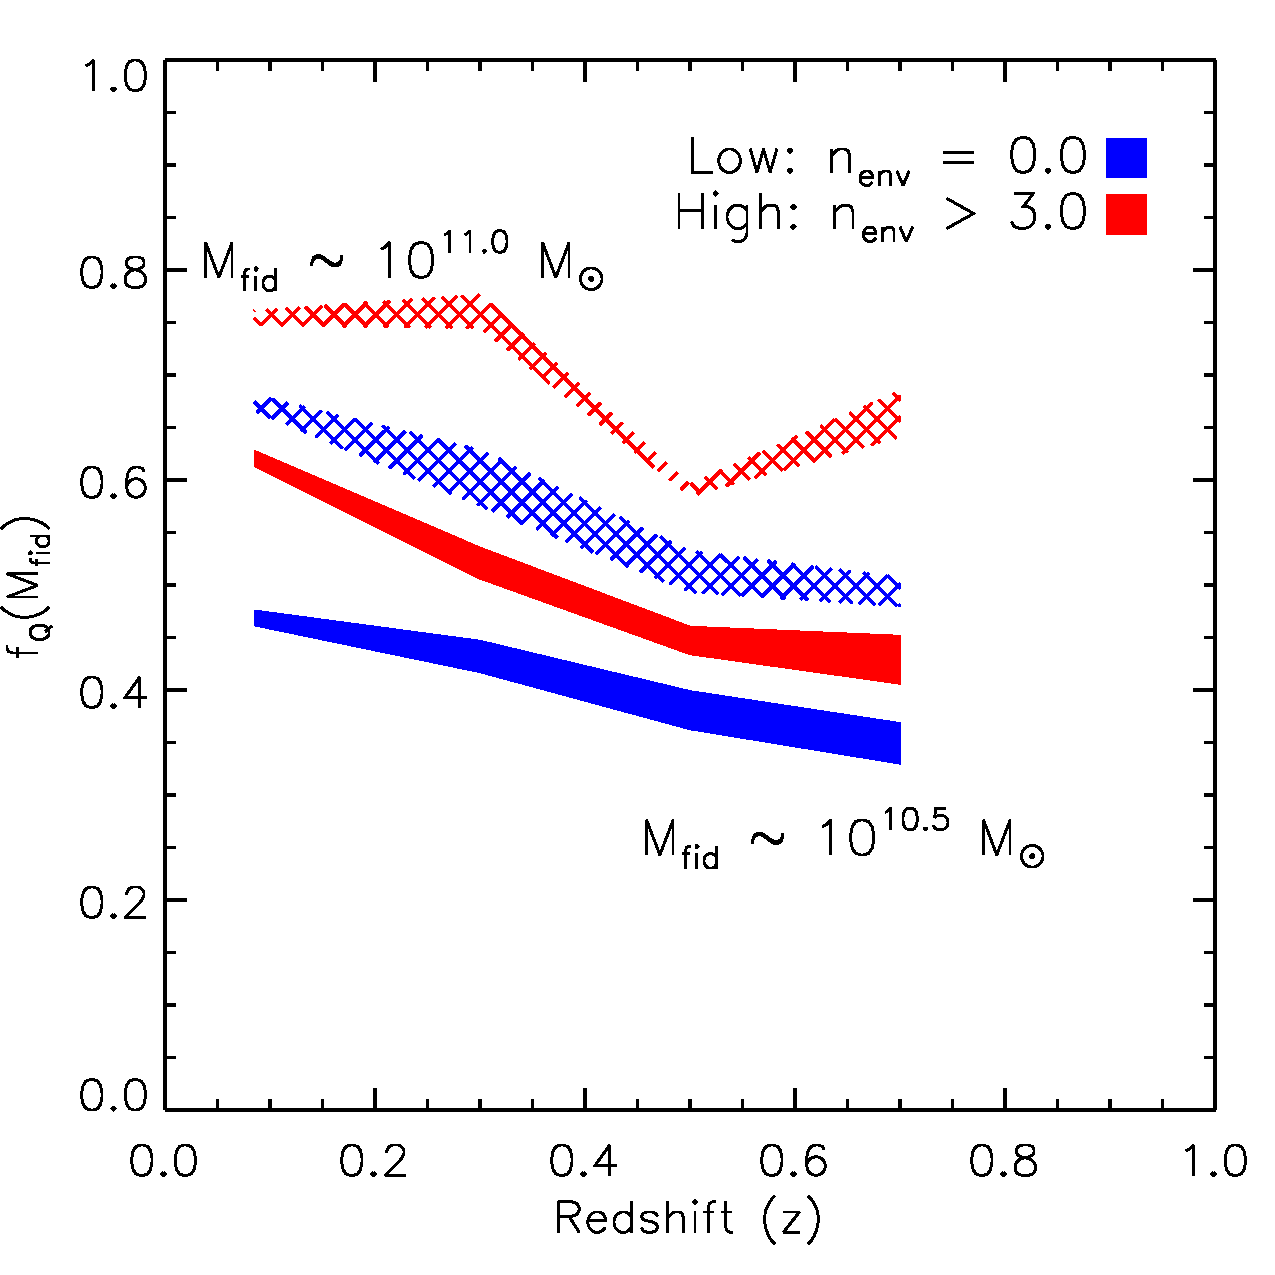
\includegraphics[width=\textwidth]{figs/qfenv/fig5.pdf}
\caption{The evolution of the quiescent fraction at fiducial
  mass, $f_{Q}(\mathcal{M}_{\mathrm{fid}})$, for low (blue) and
  high (red) density environments within the redshift range $z
  = 0.0 - 0.8$. We present the $f_{Q}(\mathcal{M}_{\mathrm{fid}})$
  evolution for $\mathcal{M}_{\mathrm{fid}} = 10^{10.5}
  \mathcal{M}_\odot$ (solid fill) and $10^{11}
  \mathcal{M}_\odot$ (patterned fill) with the uncertainty of
  the best-fit parameter $b$ in Equation \ref{eq:qffit}
  represented by the width of the line. While the high density $f_{\mathrm{Q}}(\mathcal{M}_{\mathrm{fid}})$ is greater than low density environment $f_{\mathrm{Q}}(\mathcal{M}_{\mathrm{fid}})$ over the entire redshift range of our sample, there is a significant increase in $f_{\mathrm{Q}}(\mathcal{M}_{\mathrm{fid}})$ over cosmic time for both environments. For the environment cut-offs ($n_{\mathrm{env}} =0.0 $ for low and $n_{\mathrm{env}} > 3.0$ for high), there is no significant difference in the slope of the evolution between the environments.}         \label{fig:qffit}
\end{center}
\end{figure}

\begin{table} 
  \caption{Best Fit Parameters for $f_{\mathrm{Q}}(\mathcal{M}_{*})$ Fit}
  \label{tab:bestfitparam}
  \begin{center}
    \leavevmode
    \begin{tabular}{clcc} \hline \hline              
    $z_1 < z < z_2$ &Environment        &a  &b  \\ \hline 
$0.05 < z< 0.12$ &$n_{\mathrm{env}} = \lowenvthresh$ & $0.410 \pm 0.018$ & $0.469 \pm 0.007$ \\
               &$n_{\mathrm{env}} > \highenvthresh$ & $0.270 \pm 0.016$ & $0.620 \pm 0.008$ \\ 
                              &               &                       &                           \\ \hline   
$0.2 < z <0.4$ & $n_{\mathrm{env}} = \lowenvthresh$ & $0.340 \pm 0.032$ & $0.432 \pm 0.015$ \\
               &$n_{\mathrm{env}} > \highenvthresh$ & $0.432 \pm 0.018$ & $0.544 \pm 0.010$ \\
               &               &                       &                           \\ \hline
$0.4 < z < 0.6$      &$n_{\mathrm{env}} = \lowenvthresh$ & $0.263 \pm 0.038$ & $0.381 \pm 0.018$ \\
               &$n_{\mathrm{env}} > \highenvthresh$ & $0.289 \pm 0.018$ & $0.446 \pm 0.013$ \\
               &               &                       &                           \\ \hline
$0.6 < z < 0.8$      &$n_{\mathrm{env}} = \lowenvthresh$ & $0.284 \pm 0.036$ & $0.352 \pm 0.019$ \\
               &$n_{\mathrm{env}} > \highenvthresh$            & $0.468 \pm 0.065$ & $0.429 \pm 0.023$ \\
               &               &                       &                           \\ \hline
  \multicolumn{4}{l}{}                                             \\       
    \end{tabular} \par
    \end{center}
%    \bigskip 
    {\bf Notes}: Best fit parameters in Equation \ref{eq:qffit} for each subsample $f_{\mathrm{Q}}(\mathcal{M}_{*})$ in Figure \ref{fig:qf} for $\mathcal{M}_{\mathrm{fid}} = 10^{10.5} \mathcal{M}_{\odot}$.
\end{table}

%%%%%%%%%%%%%%%%%%%%%%%%%%%%%%%%%%%%%%%%%%%%%%%%%%%%%%%%%%%%%%%%%%%%%%%%%%%%%%%%%%%%
% ENVIRONMENTAL EFFECTS ON THE QUIESCENT FRACTION EVOLUTION
%%%%%%%%%%%%%%%%%%%%%%%%%%%%%%%%%%%%%%%%%%%%%%%%%%%%%%%%%%%%%%%%%%%%%%%%%%%%%%%%%%%%
\subsection{Environmental Effects on the Quiescent Fraction Evolution} \label{sec:env_qf_evol}
In order to more quantitatively compare the $f_{\mathrm{Q}}$ evolution for different epochs and environments, we fit $f_{\mathrm{Q}}$ for each subsample to a power-law parameterization as a function of stellar mass, 
\begin{equation} \label{eq:qffit}
f_{\mathrm{Q}}(\mathcal{M}_{*}) = a \: \mathrm{log} \; \left(\frac{ \mathcal{M}_{*}}{\mathcal{M}_{\mathrm{fid}}} \right)+b,
\end{equation}
where $a$ and $b$ are best-fit parameters using {\em MPFIT} (\citealt{Markwardt:2009aa}) and $\mathcal{M}_{\mathrm{fid}}$ represents the empirically selected fiducial mass within the stellar mass limits where there is a sufficiently large number of galaxies. We primarily focus on $\mathcal{M}_{\mathrm{fid}} = 10^{10.5} \: \mathcal{M}_{\odot}$. 

In Figure \ref{fig:qffit} we present the evolution of
$f_{\mathrm{Q}}(\mathcal{M}_{\mathrm{fid}})$ from $z \sim 0.7$ to $\sim 0.1$
at low (blue) and high (red) density environments for
$\mathcal{M}_{\mathrm{fid}} = 10^{10.5} \: \mathcal{M}_{\odot}$ (solid
fill) and $10^{11} \: \mathcal{M}_{\odot}$ (pattern fill). The width
of the evolution represents the uncertainty derived from {\em
  MPFIT}. As noted earlier in Section \ref{sec:qfevol}, $f_{\mathrm{Q}}$
in high density environments is significantly greater than
$f_{\mathrm{Q}}$ in low density environments for both fiducial mass
choices. Throughout our sample's redshift range
$f_{\mathrm{Q}}(\mathcal{M}_{\mathrm{fid}})_{\mathrm{high}} -
f_{\mathrm{Q}}(\mathcal{M}_{\mathrm{fid}})_{\mathrm{low}} \sim 0.1$.

In addition, the $f_{\mathrm{Q}}(\mathcal{M}_{\mathrm{fid}})$
evolution illustrates that the quiescent fraction in low density
environment increases over cosmic time:
$f_{\mathrm{Q}}(\mathcal{M}_{\mathrm{fid}}, z \sim 0.1) -
f_{\mathrm{Q}}(\mathcal{M}_{\mathrm{fid}}, z \sim 0.7) \sim 0.1$. This
significant quiescent fraction evolution for low density environments
suggests that internal mechanisms, independent of environment, are
responsible for a significant amount of star-formation cessation. Meanwhile, the $f_{\mathrm{Q}}(\mathcal{M}_{\mathrm{fid}})$ evolution in high density environment ($f_{\mathrm{Q}}(\mathcal{M}_{\mathrm{fid}}, z \sim 0.1) - f_{\mathrm{Q}}(\mathcal{M}_{\mathrm{fid}}, z \sim 0.7) \sim 0.12$) shows little additional evolution.

When we increase our choice of $\mathcal{M}_{\mathrm{fid}}$ to $10^{11}
\mathcal{M}_\odot$, aside from an overall shift in
$f_{\mathrm{Q}}(\mathcal{M}_{\mathrm{fid}})$ by $\sim 0.2$, we observe the
same evolutionary trends. $f_{\mathrm{Q}}(\mathcal{M}_{\mathrm{fid}} =
10^{11}\mathcal{M}_{\odot})$ for both low and high density
environments each increase by $\sim 0.2$ from at all redshifts we
study. Increasing the fiducial mass to $10^{11}
\mathcal{M}_{\odot}$ does not significantly alter the evolutionary
trends in either environment. Although the varying stellar mass
completeness at each redshift bin limits the masses we probe for the
$f_{\mathrm{Q}}$ evolution, our $f_{\mathrm{Q}}$ evolution exhibits little
mass dependence.

However, the uncertainties in the PRIMUS redshifts may contaminate 
our fixed aperture measurements of galaxy environment. Consequently, we consider in Figure
\ref{fig:qffit_comp} more stringent high density environment
classifications, extending the cut off to $n_{\mathrm{env}} > 5$ and
$7$ (specified in the top right legend and represented by the color of
the shading). Aside from the increase in uncertainties that accompany
the decrease in sample size of the purer high environment sample, we
find an extension of the $f_{\mathrm{Q}}$ difference between the
environments we stated earlier. A more stringent high environment
classification significantly increases the overall
$f_{\mathrm{Q}}(\mathcal{M}_{\mathrm{fid}})$, which rises monotonically with
the $n_{\mathrm{env}}$ limit.

More importantly, a purer high environment classification reveals a
more significant environment dependence on the $f_{\mathrm{Q}}$
evolution. While the difference between the $f_{\mathrm{Q}}$ evolution in
low and high density environment is negligible for the $n_{\mathrm{env}} >
3$ cut-off, there is a notable difference in $f_{\mathrm{Q}}$
evolution between our highest cut-off $n_{\mathrm{env}} > 7$ and our low
density environment. $f_{\mathrm{Q}}(\mathcal{M}_{\mathrm{fid}}, z
\sim 0.1) - f_{\mathrm{Q}}(\mathcal{M}_{\mathrm{fid}}, z \sim 0.7)
\sim 0.25$ for $n_{\mathrm{env}} > 7$ versus
$f_{\mathrm{Q}}(\mathcal{M}_{\mathrm{fid}}, z \sim 0.1) -
f_{\mathrm{Q}}(\mathcal{M}_{\mathrm{fid}}, z \sim 0.7) \sim 0.1$ for
low density environment. In addition to the
environment independent internal mechanisms that can explain the
$f_{\mathrm{Q}}$ evolution in low density environments, there may be other
environment dependent mechanisms that can account for the moderate
environment dependence of the $f_{\mathrm{Q}}$ evolution. Our measured
difference in the $f_{\mathrm{Q}}$ evolution between environments provides
an important constraint for any environmental models for ending star
formation.

\def \iovinopanel {b}
\def \kovacpanel {b}
\def \pengpanel {c}
\begin{figure*}
\begin{center}
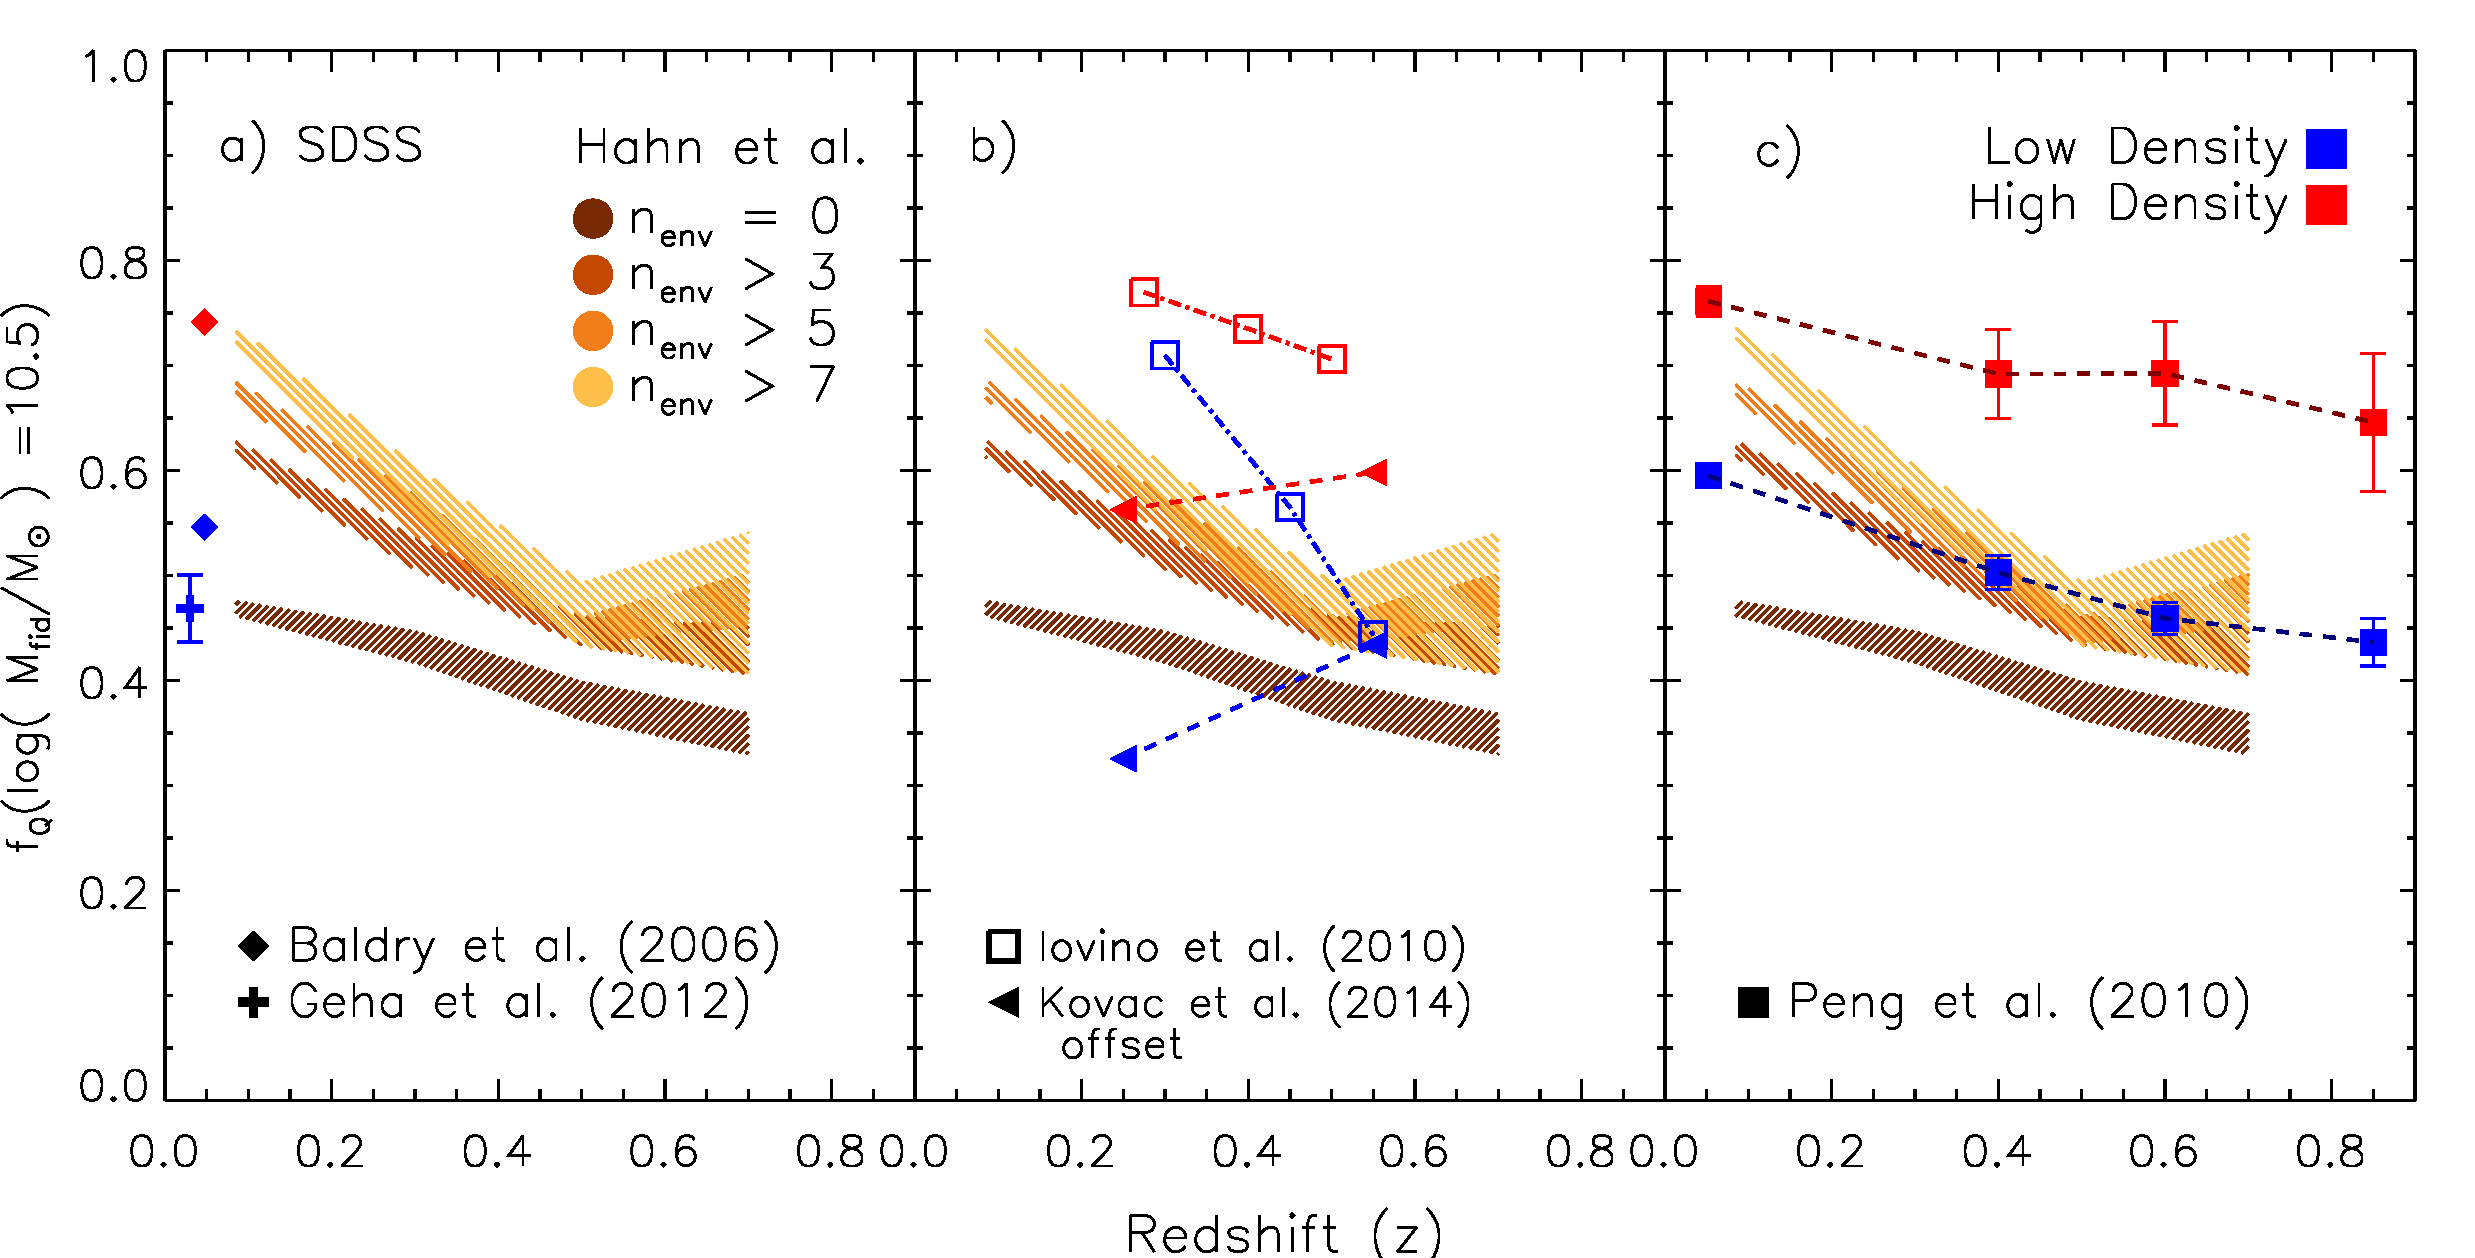
\includegraphics[width=\textwidth]{figs/qfenv/fig6.pdf}
\caption{$f_{\mathrm{Q}}(\mathcal{M}_{\mathrm{fid}}=10^{10.5} \mathcal{M}_\odot)$ evolution compared to $f_{\mathrm{red}}(\mathcal{M}_{*} \sim 10^{10.5} \; \mathcal{M}_{\odot})$ in the literature: \cite{Baldry:2006aa} (diamond) and \cite{geha12a} (cross) from SDSS (panel a), \cite{Iovino:2010aa} (empty square) and \cite{Kovac:2014aa} (triangle) from zCOSMOS (panel \kovacpanel), and \cite{Peng:2010aa} from both SDSS and zCOSMOS (panel \pengpanel). The $f_{\mathrm{red}}$ values from \cite{Iovino:2010aa}, \cite{Kovac:2014aa}, \cite{Baldry:2006aa}, and \cite{Peng:2010aa} are calculated from the best-fit parameterizations presented in the respective works. High density environment is represented in red and low density environment is represented in blue. The $f_{\mathrm{Q}}$ value from \cite{geha12a} is the $f_{\mathrm{Q}}$ value at $\mathcal{M} = 10^{10.55} \mathcal{M}_{\odot}$. Uncertainties in the \cite{Iovino:2010aa} best-fit $f_{\mathrm{red}}$ is omitted due to insufficient information on the cross correlation terms of the fit parameters. For \cite{Kovac:2014aa} we apply the offset between the color-based and SFR-based galaxy classification in order to plot the $f_{\mathrm{Q}}$ estimates. We also plot the $f_{\mathrm{Q}}(\mathcal{M}_{\mathrm{fid}} = 10^{10.5} \mathcal{M}_\odot)$ evolution of our sample with varying environment cut-offs specified on the top right. As in Figure \ref{fig:qffit} the width of the $f_{\mathrm{Q}}(\mathcal{M}_{\mathrm{fid}} = 10^{10.5} \mathcal{M}_\odot)$ evolution represent the uncertainty in the best-fit parameters of Equation \ref{eq:qffit}.}         \label{fig:qffit_comp}
\end{center}
\end{figure*}

%%%%%%%%%%%%%%%%%%%%%%%%%%%%%%%%%%%%%%%%%%%%%%%%%%%%%%%%%%%%%%%%%%%%%%%%%%%%%%%%%%%%
% COMPARISON TO LITERATURE
%%%%%%%%%%%%%%%%%%%%%%%%%%%%%%%%%%%%%%%%%%%%%%%%%%%%%%%%%%%%%%%%%%%%%%%%%%%%%%%%%%%%
\subsection{Comparison to Literature}
Although a direct comparison with other results is difficult due to
our sample specific methodology, a number of results from the literature have investigated the quiescent fraction in comparable fashions. In this section we compare our $f_{\mathrm{Q}}$ results from above to a number of these results, specifically from SDSS and zCOSMOS, with similarly defined samples and analogous environment classifications. 

In Figure \ref{fig:qffit_comp}, we plot  best-fit parameterization of
$f_{\mathrm{red}}$ for high and low density environment from SDSS (panel a), zCOSMOS (panel \iovinopanel), and \cite{Peng:2010aa} (filled square; panel d) from both surveys. 
%$f_{\mathrm{red}}$ for high and low density environment from SDSS (panel a), \cite{Baldry:2006aa} (diamond) and \cite{geha12a} (cross), zCOSMOS (panel b),
%\cite{Iovino:2010aa} (empty square) and \cite{Kovac:2014aa} (triangle), and \cite{Peng:2010aa} (filled square; panel c) from both surveys. From
From \cite{Iovino:2010aa} (empty square; panel \iovinopanel), we calculate $f_{\mathrm{red}} = 1-f_{\mathrm{blue}}$
using the best-fit $f_{\mathrm{blue}}$ from the mass bin $\mathcal{M} =
10^{10.3} - 10^{10.8} \mathcal{M}_{\odot}$. From \cite{Kovac:2014aa} (triangle; panel \kovacpanel)
we plot an estimated $f_{\mathrm{Q}}$ by applying the residual between SFR
based and color based galaxy classifications to the best-fit
$f_{\mathrm{red}}$ at $\mathcal{M} = 10^{10.5} \mathcal{M}_{\odot}$ for
low ($\delta = 0.0$) and high density environments ($\delta =
1.5$). Similarly, from \cite{Baldry:2006aa} (diamond; panel a) we plot $f_{\mathrm{Q}}$
derived from the best-fit $f_{\mathrm{red}}$ at $\mathcal{M} = 10^{10.5}
\mathcal{M}_{\odot}$ for low ($\delta = 0.0$) and high density
environment ($\delta = 1.0$). For \cite{geha12a} (cross; panel a), we plot $f_{\mathrm{Q}}$
for their isolated galaxy sample in their mass bin closest to $10^{10.5} \mathcal{M}_{\odot}$, $\mathcal{M} = 10^{10.55} \mathcal{M}_{\odot}$. Finally for \cite{Peng:2010aa} (square; panel \pengpanel), we plot the parameterized $f_{\mathrm{red}}$ at $\mathcal{M} = 10^{10.5} \mathcal{M}_{\odot}$ using their best-fit parameters for low ($\delta =0.0$) and high ($\delta = 1.4$) density environments. 

For our lowest redshift bin SDSS sample, we find that our $f_{\mathrm{Q}}$
for low and high environments are consistent with other SDSS
$f_{\mathrm{Q}}$ (or $f_{\mathrm{red}}$) measurements as a function of
environment. For example, \cite{Baldry:2006aa} uses projected neighbor
density environment measures ($\mathrm{log} \; \Sigma$) to obtain
$f_{\mathrm{Q}}(\mathcal{M})$ for a range of environmental
densities. Although the different environment measurements make direct
comparisons difficult, in their corresponding higher environments
($\mathrm{log} \; \Sigma > 0.2$ in \citealt{Baldry:2006aa})
$f_{\mathrm{Q}}(\mathcal{M} \sim 10^{10.2} \mathcal{M}_{\odot}) \sim 0.6$
and $f_{\mathrm{Q}}(\mathcal{M} \sim 10^{11.5} \mathcal{M}_{\odot}) \sim
0.9$, which is in agreement with our high density
environment. Likewise, for lower environments ($\mathrm{log} \; \Sigma <
-0.4$ in \citealt{Baldry:2006aa}) $f_{\mathrm{Q}}(\mathcal{M} \sim
10^{10.2} \mathcal{M}_{\odot}) \sim 0.4$ and $f_{\mathrm{Q}}(\mathcal{M}
\sim 10^{11.5} \mathcal{M}_{\odot}) \sim 0.8$, which also agree with
our low density environment $f_{\mathrm{Q}}$. The \cite{Baldry:2006aa}
points (diamond) in Figure \ref{fig:qffit_comp} reflect this
agreement.

More recently, \cite{Tinker:2011aa}, using a group-finding algorithm on the SDSS DR7, presents the relationship between $f_{\mathrm{Q}}$ and overdensity for galaxies within the mass range $\mathrm{log} \; \mathcal{M} = [9.8, 10.1]$. The \cite{Tinker:2011aa} $f_{\mathrm{Q}}$ at the lowest and highest overdensities, $f_{\mathrm{Q}} \sim 0.4$ and $f_{\mathrm{Q}} \sim 0.6$ respectively, are consistent with our $f_{\mathrm{Q}}$ for low and high density environment at the lower mass limit ($\mathrm{log} \; \mathcal{M} \sim 10.2$). 

A modified \cite{Tinker:2011aa} sample is used in \cite{geha12a} to
obtain $f_{\mathrm{Q}}$ for isolated galaxies over a wider mass range
($10^{7.4} \mathcal{M}_\odot$ to $10^{11.2}
\mathcal{M}_{\odot}$). Although \cite{geha12a} probe a slightly lower
redshift range ($ z \le 0.06$), their $f_{\mathrm{Q}}$ is consistent with
our low density sample. Within the overlapping mass range, at the low
mass end \cite{geha12a} find $f_{\mathrm{Q}}(\mathcal{M}_{*} \sim
10^{10.2} \mathcal{M}_{\odot}) \sim 0.3$ and at the high mass end they
find $f_{\mathrm{Q}}(\mathcal{M}_{*} \sim 10^{11.2} \mathcal{M}_{\odot})
\sim 0.8$. Both of these values agree with our lowest redshift
$f_{\mathrm{Q}}$ results in low density environment. Figure
\ref{fig:qffit_comp} illustrates the $f_{\mathrm{Q}}$ agreement for
$\mathcal{M}_{*} = 10^{10.5} \mathcal{M}_{\odot}$.

%\cite{Peng:2010aa} computes the comoving density field for the SDSS DR7 and zCOSMOS galaxies in order to calculate $f_{\mathrm{red}}$ as a function of mass and environment. If we compare our $f_{\mathrm{Q}}$ to the best-fit parameterization $f_{\mathrm{red}}$ for their SDSS subsample we find that 

For $z > 0.2$, we compare our PRIMUS $f_{\mathrm{Q}}$ results to the $f_{\mathrm{red}}$ (or $1-f_{\mathrm{blue}}$) results from the zCOSMOS Redshift Survey (\citealt{Iovino:2010aa, Kovac:2014aa}), which covers a similar redshift range as PRIMUS. \cite{Iovino:2010aa}, and \cite{Kovac:2014aa} using a mass-complete galaxy sample derived from zCOSMOS and a group catalog, 3D local density contrast, and overdensity environment measurements, respectively, compare $f_{\mathrm{red}}$ with respect to environment. The $f_{\mathrm{blue}}$ for group and isolated galaxies from \cite{Iovino:2010aa} are generally inconsistent with our $1-f_{\mathrm{Q}}$ for high and low density environments. 

Similarly, $f_{\mathrm{red}}$ for high and low overdensities in
\cite{Kovac:2014aa} are  greater overall than the PRIMUS $f_{\mathrm{Q}}$
values in high and low density environments. However,
\cite{Kovac:2014aa} points out that there is a significant difference
between classifying the quiescent population using color and SFR due to dust-reddening in star-forming galaxies. For their lower redshift bin ($0.1 < z < 0.4$) \cite{Kovac:2014aa} find that their $f_{\mathrm{Q}}$ defined by color is greater than $f_{\mathrm{Q}}$ defined by SFR by roughly $0.2$. While for their higher redshift bin ($0.4 < z < 0.7$) the difference is $0.15-0.19$. Although \cite{Kovac:2014aa} does not elaborate on how the galaxy classification discrepancy applies to the different environments, if we simply account for the difference uniformly for $f_{\mathrm{red}}$ at all environments, the \cite{Kovac:2014aa} results in their lower redshift bin are roughly consistent with our $f_{\mathrm{Q}}$ at high and low density environments. Even accounting for the dust-reddening of $f_{\mathrm{red}}$, \cite{Kovac:2014aa} finds a significantly higher $f_{\mathrm{Q}}$ in their higher redshift bin. 

In Figure \ref{fig:qf}, the $f_{\mathrm{Q}}$ evolution with respect to
mass reveals, qualitatively, little mass dependence in the
evolution. Moreover, in Figure \ref{fig:qffit}, we illustrated that
adjusting the fiducial mass only shifted the overall
$f_{\mathrm{Q}}(\mathcal{M}_{\mathrm{fid}})$, but did not change the
$f_{\mathrm{Q}}$ evolutionary trend. The consistency in the $f_{\mathrm{Q}}$
evolutionary trends over change in fiducial mass suggests that
$f_{\mathrm{Q}}$ evolution exhibit little mass dependence within the 
mass range probed in our analysis. In contrast to
the weak mass dependence we observe in our results,
\cite{Iovino:2010aa} find significantly different $f_{\mathrm{Q}}$
evolution at $\mathcal{M} \sim 10^{11} \mathcal{M}_{\odot}$ and
$\mathcal{M} \sim 10^{10.5} \mathcal{M}_{\odot}$, for both group and
isolated galaxies. In fact at their highest mass bin ($10^{10.9} -
10^{11.4} \mathcal{M}_{\odot}$), \cite{Iovino:2010aa} find no evolution
for both environments: constant $f_{\mathrm{blue}} \sim 0.1$ over $z =
0.3 - 0.8$ for both group and isolated galaxy populations.

Meanwhile in their mass bin most comparable to $\mathcal{M}_{\mathrm{fid}}
\sim 10^{10.5} \mathcal{M}_{\odot}$ ($10^{10.3} \mathcal{M}_{\odot} -
10^{10.8} \mathcal{M}_{\odot}$), \cite{Iovino:2010aa} finds that
$f_{\mathrm{blue}}$ evolves by $\sim 0.1$ from $z = 0.5$ to $0.25$ for
group galaxies and by $\sim 0.3$ from $z=0.55$ to $0.3$ for isolated
galaxies as presented in panel (\iovinopanel) of Figure \ref{fig:qffit_comp}. Altogether, with
mass bins beyond the fiducial masses we explore, \cite{Iovino:2010aa}
find a strong mass dependence with $f_{\mathrm{Q}}$ evolving significantly
more in lower mass bins. While our sample from PRIMUS provides larger
statistics than zCOSMOS, the mass-completeness limits we impose on our
sample limits the mass range we probe (e.g. $\mathcal{M} > 10^{10.5}
\mathcal{M}_{\odot}$ for our $z \sim 0.7$ bin). Consequently our
results cannot rule out mass dependence in the $f_{\mathrm{Q}}$ evolution
at lower masses.

In Figure \ref{fig:qffit} and Figure \ref{fig:qffit_comp} we
quantified that throughout our redshift range, high density
environments have a significantly greater
$f_{\mathrm{Q}}(\mathcal{M}_{\mathrm{fid}})$ than the low density
environments. This finding is in agreement with the zCOSMOS results
from \cite{Cucciati:2010aa} and \cite{Kovac:2014aa}. As illustrated in
panel (\kovacpanel) of Figure \ref{fig:qffit_comp}, \cite{Kovac:2014aa} finds $f_{\mathrm{Q}}$ in high density environment
significantly greater than $f_{\mathrm{Q}}$ at low density
environment. Moreover, since galaxy color serves as a proxy for SFR,
our results support the existence of the color-density relation
(\citealt{Cucciati:2010aa, Cooper:2010aa}) and is not consistent with
the color-density relation being merely a reflection of the
mass-density relationship, as \cite{Scodeggio:2009aa} suggest it is
based on the Vimos VLT Deep Survey ($0.2 < z< 1.4$).

% Purposely not mentioning the lack of morphology-density relation for M>10^10.5Msun galaxies as argued in Tasca et al. 2009 in order to not bring up morphology. 

In Section \ref{sec:env_qf_evol}, we showed that $f_{\mathrm{Q}}$ in
low density environments evolves over cosmic time. From this trend we
deduce that internal, environment independent, mechanisms contribute
to ending star-formation in galaxy evolution. \cite{Iovino:2010aa}
from zCOSMOS, plotted in Figure \ref{fig:qffit_comp}  panel (\iovinopanel), also find that
$f_{\mathrm{Q}}$ in low density environment increases with decreasing redshift. On the other hand \cite{Kovac:2014aa}, also from zCOSMOS, presents that $f_{\mathrm{Q}}$ in low density environment decreases over cosmic time. While the uncertainties for the parameterized $f_{\mathrm{Q}}$ are not listed, and thus not shown in Figure \ref{fig:qffit_comp}, once they are accounted for, \cite{Kovac:2014aa} find no significant $f_{\mathrm{Q}}$ evolution over cosmic time. However, once we account for the dust-reddening of the $f_{\mathrm{red}}$, we find a more significant decrease over cosmic time (Figure \ref{fig:qffit_comp} panel \kovacpanel).

Furthermore, in Section \ref{sec:env_qf_evol}, our comparison of the
$f_{\mathrm{Q}}$ evolution between the lowest density environment and the
highest density environment revealed a modicum of evidence for the
existence of environment dependent mechanisms. The same comparison
with zCOSMOS results (\citealt{Iovino:2010aa, Kovac:2014aa}) present
trends inconsistent with our findings. First, comparing the high (red)
and low (blue) density environments for \cite{Iovino:2010aa} in Figure
\ref{fig:qffit_comp} shows that there are indeed pronounced
discrepancies between the $f_{\mathrm{Q}}$ evolution in different
environments. Group galaxies in \cite{Iovino:2010aa} have higher
overall $f_{\mathrm{Q}}$ than isolated galaxies. However, unlike our
results, which find a greater $f_{\mathrm{Q}}$ evolution at higher density
environments, $f_\mathrm{Q}$ in \cite{Iovino:2010aa} shows the opposite environment
dependence that there is a significantly greater $f_{\mathrm{Q}}$
evolution for isolated galaxies. Once the large uncertainties in the $f_\mathrm{Q}$ 
fit are taken into account, \cite{Iovino:2010aa} state that the $f_\mathrm{Q}$ is difficult to measure from their sample. 

Next, \cite{Kovac:2014aa} also find that overall $f_{\mathrm{Q}}$ is
greater in high density than in low density environments. Like their
low density environment $f_{\mathrm{Q}}$ evolution, $f_{\mathrm{Q}}$ in high
density environment decreases over cosmic time between their two
redshift bins. Although the decrease in $f_{\mathrm{Q}}$ over cosmic time
conflicts with our results, \cite{Kovac:2014aa} finds a greater (less
negative) $f_{\mathrm{Q}}$ evolution in high density environments relative
to low density environments, suggesting an environment dependence that
is in the same direction as our results. We note that the negative
slopes of the $f_{\mathrm{Q}}$ evolution in both environments are enhanced
in Figure \ref{fig:qffit_comp} due to the dust-reddening
correction we impose to the \cite{Kovac:2014aa} $f_{\mathrm{red}}$ results. 

%However, even without the correction (not shown), in their best-fit $f_{\mathrm{Q}}$ results, the same evolutionary trends mentioned above are observed. 

Due to the redshift uncertainties in PRIMUS, our galaxy environment measures are more susceptible to contamination. As discussed in \cite{Coil:2011aa} and \cite{Cool:2013aa}, PRIMUS has redshift success rate of $> 75 \%$; in comparison, zCOSMOS has $88 \%$ redshift completeness for the entire sample and $95 \%$ complete within the redshift range $0.5 < z < 0.8$ (\citealt{Lilly:2009aa}). Although the zCOSMOS survey provides more precise spectroscopic redshifts, PRIMUS has higher overall completeness due to its high targeting fraction of $\sim 80 \%$. zCOSMOS has a spatial sampling rate of $\sim 30-50\%$ and a overall completeness rate of $48 - 52 \%$ (\citealt{Knobel:2012aa}). Our sample also provides larger statistics and covers a larger portion of the sky. Our SDSS-{\em GALEX} sample covers $2,505 \;\mathrm{deg}^2$. More comparably, our PRIMUS sample covers $5.5 \;\mathrm{deg}^2$, over 3 times the sky coverage of zCOSMOS ($1.7 \;\mathrm{deg}^2$). Furthermore, our PRIMUS sample is constructed from five independent fields which allows us to significantly reduce the effects of cosmic variance.

As listed in Table \ref{tab:subsample}, after our edge effect cuts and
stellar mass completeness limits, our sample consists of $13,734$
galaxies from PRIMUS over $0.2< z< 0.8$ and $63,417$ galaxies from
SDSS over $0.05 < z < 0.12$. Meanwhile, \cite{Iovino:2010aa} has $914$
galaxies with $\mathcal{M} > 10^{10.3} \mathcal{M}_{\odot}$ over $0.1
< z < 0.6$ and $1033$ galaxies with $\mathcal{M} > 10^{10.6}
\mathcal{M}_{\odot}$ over $0.1 < z < 0.8$. For the actual sample used
to obtain the best-fit $f_{\mathrm{Q}}$ values in Figure
\ref{fig:qffit_comp} \cite{Iovino:2010aa} has $617$ galaxies. In
comparison, our PRIMUS sample alone contains $> 20$ times the number
of galaxies. While there is a considerable difference in the overall
$f_{\mathrm{Q}}$ between our results and those of \cite{Iovino:2010aa},
the use of different methodologies, particularly for galaxy
classification and environment measurements, make such comparisons
ambiguous. On the other hand, the discrepancies in the $f_{\mathrm{Q}}$
evolutionary trends with our results may be explained by the limited
statistics in the \cite{Iovino:2010aa} sample.

The more recent \cite{Kovac:2014aa} provides larger statistics with
$2,340$ galaxies in their lower redshift bin ($0.1 < z < 0.4$) and
$2,448$ galaxies in their higher redshift bin ($0.4 < z <
0.7$). Although their sample is smaller than the PRIMUS sample, which
contains over twice times the number of galaxies, the
\cite{Kovac:2014aa} sample provides a more stable comparison.  Once
their results are adjusted for the dust-reddening, we
find that their overall $f_{\mathrm{Q}}$ is more or less consistent with
our overall $f_{\mathrm{Q}}$. However, it is difficult to explain the
significant discrepancies in the $f_{\mathrm{Q}}$ evolutionary trends.
The significant overdenities observed in the COSMOS field at $z \sim 0.35$ and $z \sim 0.7$ (\citealt{Lilly:2009aa, Kovac:2010ab}) may have a significant effect on the zCOSMOS results and offer a possible explanation for the discrepancies. 
% zCOSMOS has more precise redshift but PRIMUS has it beat in terms of sample size and coverage of the sky 5.5 deg^2 vs 1.7 deg^2
% Kovac: 1.7 deg^2, 0.1 < z < 0.4 2340 and 0.4 < z < 0.7 2448. Most of the data points have errors of +/- 0.1, at least +/-0.05
% Iovino: 1.7 deg^2  617 galaxies in 10.3 < M < 10.8 and 0.1 < z < 0.6. Errors are +/1 0.1

%%%%%%%%%%%%%%%%%%%%%%%%%%%%%%%%%%%%%%%%%%%%%%%%%%%%%%%%%%%%%%%%%%%%%%%%%%%%%%%%%%%%
% SUMMARY
%%%%%%%%%%%%%%%%%%%%%%%%%%%%%%%%%%%%%%%%%%%%%%%%%%%%%%%%%%%%%%%%%%%%%%%%%%%%%%%%%%%%
\section{Summary and Discussion} \label{sec:summary}
Using a stellar mass complete galaxy sample derived from SDSS and
PRIMUS accompanied by a consistently measured galaxy environment from
robust spectroscopic redshifts, we measure the stellar mass functions
for star-forming and quiescent galaxies in low and high density
environments over the redshift range $0.05 < z < 0.8$. From these
stellar mass functions, we compare the proportion of galaxies that
have ended their star-formation within the subsamples by computing the
quiescent fraction for each of them. In order to better quantify the
evolution of the quiescent fraction over cosmic time, we fit our
quiescent fraction anchored at a fiducial mass. 

From our analyses we find the following notable results. The first
three demonstrate that previous findings that are well known in the
local universe are applicable out to $z\sim 0.7$. The last two are
consistent with the findings of \cite{Peng:2010aa} but provide increased
detail on the environmental dependence of galaxy evolution:
\begin{enumerate}
	\item From the SMFs, we find that the galaxy population in high
    density environments, both star-forming and quiescent, have a
    higher median mass, thus confirming the mass-density relation and
    mass-segregation in different environments throughout our sample's
    redshift range.
	\item For all subsamples, $f_{\mathrm{Q}}$ increases monotonically with
    galaxy stellar mass, showing a clear mass dependence and
    reflecting the well-established color-mass and morphology-mass
    relations.
	\item We illustrate that $f_{\mathrm{Q}}$ in high density environments
    is greater than $f_{\mathrm{Q}}$ in low density environments
    for $\mathcal{M} \sim 10^{10.5} -10^{11} \mathcal{M}_\odot$ and out to redshift $z\sim 0.7$. This result
    reflects the well known trend that galaxies in high density
    environment are statistically redder, have lower SFRs, and are
    more massive.
	\item $f_{\mathrm{Q}}$ increases significantly with redshift for both
    low and high density environments. For high density environment,
    this trend is the Butcher-Oemler effect. Furthermore, the
    $f_{\mathrm{Q}}$ evolution in low density environment suggest the
    existence of internal environment-independent mechanisms for
    ending star formation.
	\item Comparison of the $f_{\mathrm{Q}}(\mathcal{M}_{\mathrm{fid}})$
    evolution for a range of environment classifications reveals that
    the since $z = 0.8$, $f_{\mathrm{Q}}$ has evolved by a greater amount
    in the highest density environments. For our purest high
    environment sample ($n_{\mathrm{env}} > 7$), the total $f_{\mathrm{Q}}$
    evolution is $\sim 0.1$ greater than the total $f_{\mathrm{Q}}$
    evolution in low density environment, revealing a moderate
    dependence on environment.
\end{enumerate}

Many physical mechanisms have been proposed to explain the cessation
of star-formation observed in many galaxies. Recently star-formation
cessation has often been classified into internal or external
mechanisms, and sometimes more specifically into mass-dependent and
environment-dependent mechanisms (\citealt{Baldry:2006aa,
  Peng:2010aa}). The significant redshift evolution of the
$f_{\mathrm{Q}}$ in low density environments confirms the existence of
internal mechanisms that end star-forming in galaxies.

Furthermore, the greater $f_{\mathrm{Q}}$ evolution in the highest density
environment relative to low density environments suggests that in
addition to the internal mechanisms, in high density environments such
as groups and clusters, environment-dependent effects may also
contribute to the end of star-formation. Our results do not
specifically shed light on which mechanisms (e.g. strangulation,
ram-pressure stripping, etc.) occur in high density environments. Not to 
mention, the mechanism could yet be indirect; for example, the
galaxies in higher density environments could end star-formation
primarily due internal processes, which affect the galaxies that end up
in groups and clusters more greatly.  Nevertheless, our results impose
important constraints on the total possible contribution of
environment dependent mechanisms that models must satisfy, providing a
limit on the role of environment in ending star formation in
galaxies. 

\section*{Acknowledgements}
CH and MB were supported by NSF-AST-1109432 and NSF-AST-0908354. MB was also supported by NSF-AST-1211644. ALC acknowledges support from NSF CAREER award. We acknowledge Katarina Kova\u{c} and Ying-Jie Peng for  insightful discussions. We also thank Marla Geha for providing published quiescent fraction results in electronic format.

Funding for PRIMUS has been provided by NSF grants AST-0607701, 0908246, 0908442, 0908354, and NASA grant 08-ADP08-0019. The Galaxy Evolution Explorer (GALEX) is a NASA Small Explorer, launched in April 2003, whose mission was developed in cooperation with the Centre National d`Etudes Spatiales of France and the Korean Ministry of Science and Technology. Funding for the SDSS and SDSS-II has been provided by the Alfred P. Sloan Foundation, the Participating Institutions, the National Science Foundation, the U.S. Department of Energy, the National Aeronautics and Space Administration, the Japanese Monbukagakusho, the Max Planck Society, and the Higher Education Funding Council for England. The SDSS Web Site is http://www.sdss.org. The SDSS is managed by the Astrophysical Research Consortium for the Participating Institutions. 


% Conclusion
\chapter*{Conclusion}\addcontentsline{toc}{chapter}{Conclusion}
%
%\todo{
%something that references the intro and answers it  \\
%In this dissertation, we have tackled key methodological challenges 
%in galaxy clustering analyses and galaxy evolution with robust treatment of systmeatics, innovative
%approaches to inference, and improved models of the galaxy-halo 
%connection.
%} 
%
%
%\todo{Summary of \Chap{fc}}
%
%\todo{Summary of \Chap{abc}}
%
%\todo{Summary of \Chap{galenv}} % galaxy-halo connection from an observational view
%
%\todo{Summary of \Chap{galhalo}} % galaxy-haloc onnection from a data-driven LCDM view

Over the next decade future surveys, namely eBOSS and DESI, will expand the 
cosmic volumes probed with redshifts by an order of magnitude. They have the 
potential to measure the growth of structure and constrain cosmological 
parameters with unprecedented precision. The main challenges for realizing 
their full statistical power are methodological. The frameworks I present
in this dissertation -- robust treatment of systematics, innovative approaches 
to accurate inference, and improved models of the galaxy-halo connection -- can be 
extended to these future surveys and used to tackle key methodological 
challenges. 
%by robust treatment of systematics, accurate modeling, and higher order statistics.
%eBOSS and DESI will expand the cosmic volume probed with redshifts by an order of magnitude. 
%They have the potential to measure the growth of structure and \mneut~with unprecedented precision.
%eBOSS and DESI will probe unprecedented cosmic volumes with galaxy redshifts and have the potential to measure the growth of structure and \mneut~with extraordinary precision. 
%Galaxy clustering and thereby the growth of structure from RSD and \mneut ~can be measured with unprecedented precision. 
%The main obstacles for realizing the full statistical power are methodological and can be solved by robust treatment of systematics, accurate probabilistic inference, and higher order statistics.\\ \vspace{-3mm}

For instance, observational systematics such as fiber collisions will continue 
to impact galaxy clusteing analyses of eBOSS and DESI, which will utilize 
fiber-fed spectrographs. As described in~\Chap{fc}, due to the impact that fiber 
collisions have on small scales, much of the statistical gains from eBOSS and 
DESI will be {\em wasted} if they are not properly account for in analyses. 
In fact, in eBOSS and DESI the systematics will be more complicated with multiple 
classes of target objects and automated fiber positioning 
\citep{Cahn:2015_desifib, Dawson:2015aa}. But the methods from ~\Chap{fc} 
can be extended to both surveys.

Furthermore, in~\Chap{abc}, we revealed deviations between the ABC posterior 
probability distribution and the standard Gaussian pseudo-likelihood approach to 
inference -- even in the narrower context of halo occupation modeling. Yet 
there have not been direct investigations on the impact of the standard 
assumptions on more general cosmological parameter constraints. With the 
increased statistical power of future surveys, quantifying the impact of these 
assumptions in our inference is critical for unbiased constraints. While
tractability of forward modeling the data has been an obstacle for adopting 
ABC, new models aimed at the next galaxy surveys, are making promising 
strides. 

Finally, as we describe in~\Chap{galenv}, observations of galaxies have 
firmly established a global view of galaxy properties out to $z{\sim}1$. 
As in \Chap{galhalo}, precise predictions of hierarchical growth of 
structure from $\Lambda$CDM can be used to constrain key elements of 
galaxy evolution in a data-driven and statistical fashion. The introduction 
of Integral Field Unit observations (\emph{e.g.} MaNGA) and larger 
galaxy samples (\emph{e.g.} DESI Bright Galaxy Survey) offer exciting 
opportunities to extend the works of \chapname s~\chapalt{galenv} and~\chapalt{galhalo}
and construct better models of the galaxy-halo connection.

Each aspect of my dissertation will be instrumental for exploiting the full 
potential of future surveys and making more precise measurements of the growth
rate of structure, the cosmological parameters, and thus tests of General Relativity 
and modified gravity scenarios. 
%Measuring this redshift-space distortion (RSD) allows us to infer the growth of structure, which we can then use to test GR and modified gravity scenarios. 
%doubly instrumental for extracting accurate and precise \mneut ~constraints from eBOSS and DESI.
Furthermore, galaxy clustering also provides a unique window to probe 
fundamental physics --- {\em i.e.} the total neutrino mass (\mneut).
Extending the methods from my dissertation to future surveys will allow 
us to better measure the imprints of neutrinos on LSS and produce 
tigher constraints on \mneut. A tighter 
upper limit on \mneut ~is essential to distinguish between the neutrino mass 
hierarchies and will provide an important input for particle physics theory 
beyond the Standard Model.



% %%%%% Appendices start %%%%%%%%%%%%%%%%
% %% Comment out the following line if your thesis has no appendix
% \appendix
% \chapter*{Effective Window Method Polynomials \label{chap:append1}}
\addcontentsline{toc}{chapter}{Appendices}
\addcontentsline{toa}{appendix}{Appendix A}
\addtocontents{toa}{\addvspace{10pt}}%just to separate the entries in the list

For reference, here we list the first few polynomials $H_{l_> l_<}(x)$ from Eq.~(\ref{foffdiag})
\beqa
H_{20}(x)&=&x^2-1, \\ & & \nonumber \\
H_{40}(x)&=&{7\over 4}x^4-{5\over 2}x^2 +{3\over 4}, \\  & & \nonumber \\
H_{42}(x)&=&x^4-x^2, \\& & \nonumber \\
H_{60}(x)&=&    \frac{33}{8} x^6 - \frac{63}{8}x^4 + \frac{35}{8}x^2 - \frac{5}{8}  , \\ & & \nonumber \\
H_{62}(x) &=&   \frac{11}{4}x^6 - \frac{9}{2}x^4 + \frac{7}{4}x^2, \\ & & \nonumber \\
H_{64}(x) &=&  x^6 -  x^4 
\label{Hpoly}
\eeqa

% %% Note: If your thesis has more than one appendix, NYU requires a "list of
% %% appendices" page before the body of the thesis. I don't provide the tools
% %% to create that here, so you're on your own for that one... Sorry.
% %\chapter*{Indicators of Star Formation \label{chap:append2}}
\addcontentsline{toa}{appendix}{Appendix B}
\addtocontents{toa}{\addvspace{10pt}}%just to separate the entries in the list

In order to measure star formation in galaxies of the SDSS DR7 
group catalog, we use specific star formation rates (SSFR) derived
in \cite{Brinchmann:2004aa} (briefly described in \S~\ref{sec:sdss}). 
These SSFR are measured from H$\alpha$ emission lines, and 
$D_n4000$ for SSFRs$\gtrsim 10^{-12}\mathrm{yr}^{-1}$. While no 
SFR indicator provides the panacea for uncertainties in measuring
star formation in galaxies, a number of caveats must be addressed 
for the \cite{Brinchmann:2004aa} SSFR. SSFRs derived from H$\alpha$ 
probe star formation on a $\sim 10\;\mathrm{Myr}$ timescale, which 
makes them sensitive to short term varations in the galaxies' star 
formation histories \citep{Kennicutt:2012aa}. Furthermore, the 
spectroscopically derived \cite{Brinchmann:2004aa} SSFRs also 
rely on aperture corrections, which may introduce further 
uncertainties. In this section, we demonstrate, by comparing to 
another SFR indicator, that our specific choice of SFR indicator 
does not significant impact the central galaxy quenching 
timescale. 

In \cite{Moustakas:2013aa} (hereafter M2013), for their lowest redshift galaxy 
sample, they construct a catalog derived from the SDSS DR7 VAGC. 
They supplement the optical photometry from SDSS DR7 with 
UV photometry from GALEX, integrated $J\;H\;K_s$ magnitudes 
from 2MASS Extended Source Catalog, and integrated photometry 
at $3.4$ and $4.6\mu m$ from the WISE All-Sky Data Release\footnote{http://wise2.ipac.caltech.edu/docs/release/allsky}.
Then to derive galaxy properties such as $\mathcal{M}_*$ and
SFR, they use $\mathtt{iSEDfit}$ -- a Bayesian SED modeling code. 
By including UV photometry from GALEX, the SFRs from the 
M2013 catalog traces star formation over 
$\sim 10 - 100\;\mathrm{Myr}$ timescales and is not dominated
by short term variations. Furthermore, as these SFRs are 
derived from photometry, they do not require any aperture 
correction. 

Galaxies that are in both the SDSS DR7 group catalog and 
M2013 catalog, provide a convenient galaxies sample
to compare the distinct SFR indicators. In Figure~\ref{fig:Pssfr_comp}, 
we compare the SSFR distributions of this subsample, 
calculated using SSFRs from the SDSS DR7 group catalog (black dashed) 
versus M2013 (orange): $P(\mathrm{SSFR}^{\rm group})$ versus 
$P(\mathrm{SSFR}^{M2013})$. Before comparing the 
$P(\mathrm{SSFR})$s, we note that the SSFRs from M2013 are 
not subject to the \cite{Brinchmann:2004aa} SSFR upper bounds 
for low star-forming galaxies (see \S~\ref{sec:sdss}). 
That is, the M2013 SSFRs can extend
below $10^{-13}\;\mathrm{yr}^{-1}$. For a meaningful comparison, 
however, we impose similar SSFR bounds to reproduce the 
$P(\mathrm{SSFR}^{\rm group})$ quiescent peak. We also note 
that due to the M2013 bright magnitude limit, the M2013 sample 
does not contain a large number of galaxies within the group 
catalog's $z$ range at higher mass bins. Furthermore, for
both distributions, the galaxies are binned based on the
group catalog $\mathcal{M}_*$ so that the same galaxies are
examined in each bin. This binning does not have a significant
impact on the comparision because the group catalog $\mathcal{M}_*$ 
and M2013 $\mathcal{M}_*$ are tightly correlated. 
% need to mention that we're looking at the same galaxies in 
% each mass bin.

There are some minor discrepancies between the SSFR distributions, 
such as the position of the star-forming peak in the lowest mass 
bin. While this is caused by small
differences in the slopes of the SFMS between the M2013 sample 
and the group catalog, the star-forming peaks in the higher mass bins are 
in good agreement. So for the $\mathcal{M}_*$ probed by our analysis, 
this discrepancy does not have a significant impact. Overall, however, 
the $P(\mathrm{SSFR})$s are in good agreement with one another. 
Furthermore, we find that the heights of the green valley in both 
distributions, the main feature of $P(SSFR)$ critical for 
constraining the central quenching timescale, are also in good 
agreement. Therefore, we conclude that the \cite{Brinchmann:2004aa} SFRs
do not significantly impact the quenching timescale and the results of
this work. 


\begin{figure*}
\begin{center}
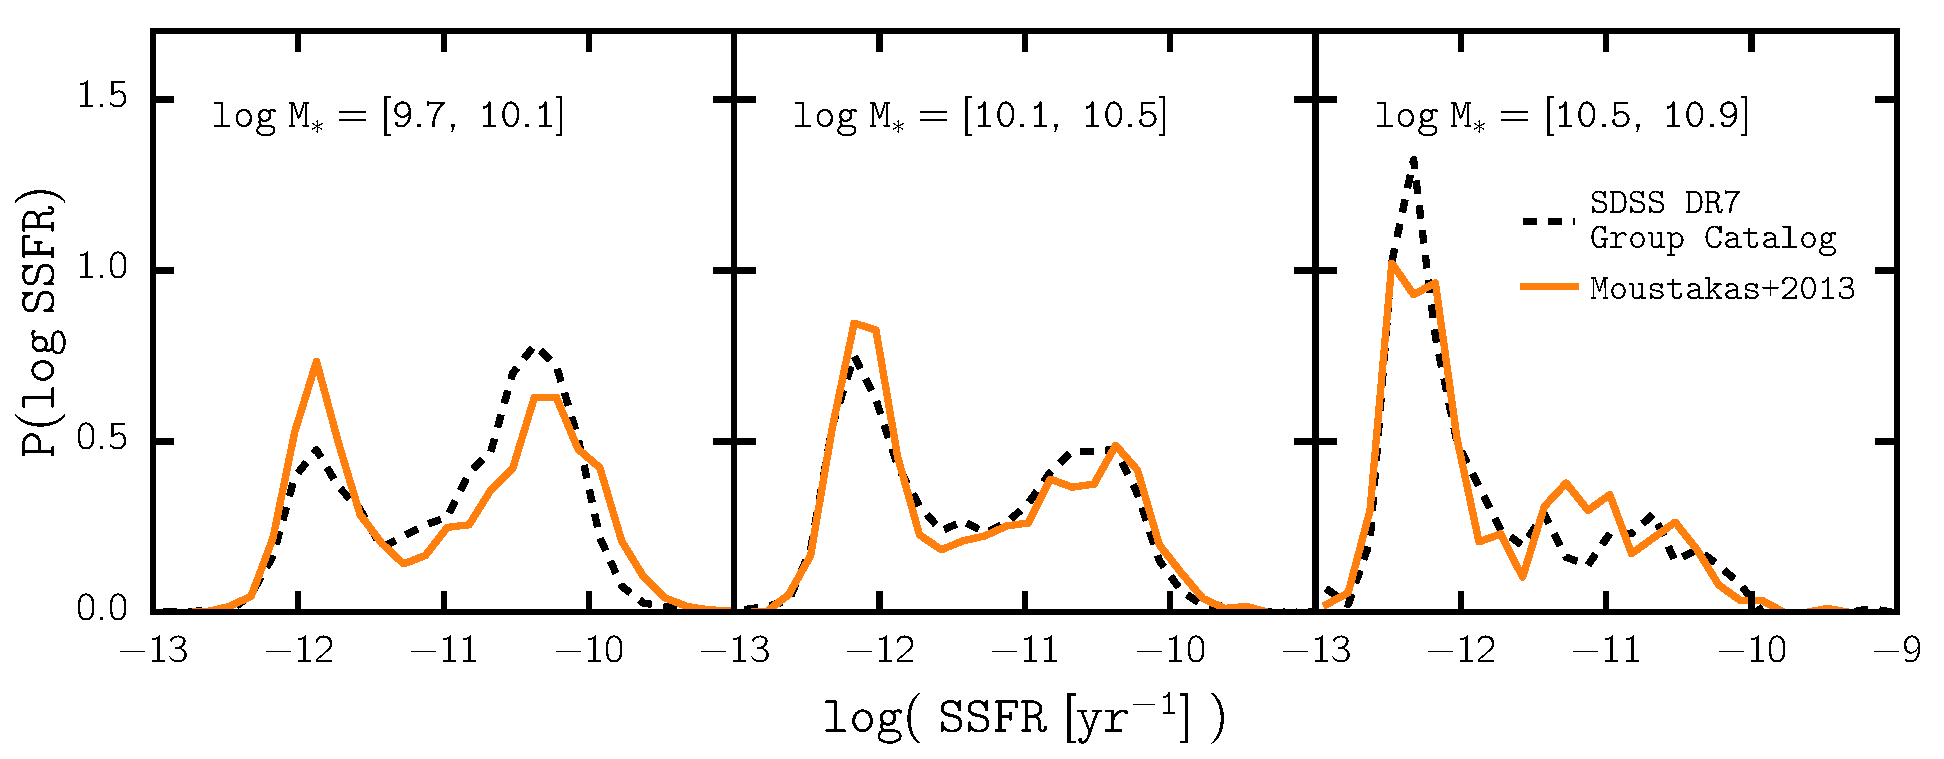
\includegraphics[width=\textwidth]{figs/cenq/Pssfr_comparison.pdf}
\caption{
Comparison of the SSFR distribution calculated using 
SSFRs from the SDSS DR7 group catalog (black dashed) versus
\cite{Moustakas:2013aa} (orange) for galaxies that are in 
both the SDSS DR7 group catalog and the \cite{Moustakas:2013aa} 
sample $z\sim0.1$ bin: $P(\mathrm{SSFR}^{\rm group})$ versus 
$P(\mathrm{SSFR}^{M2013})$. Galaxies are binned based on the
group catalog $\mathcal{M}_*$ for both distributions so that 
the same galaxies are examined in each bin. We impose SSFR 
bounds on $P(\mathrm{SSFR}^{M2013})$ for low SSFRs to reproduce 
the $P(\mathrm{SSFR}^{\rm group})$ quiescent peak (\S~\ref{sec:sdss}). 
We note that the M2013 sample does not contain a large number 
of galaxies within the group catalog's $z$ range at higher 
mass bins due its bright magnitude limit.
We find good overall agremeent between $P(\mathrm{SSFR}^{\rm group})$ 
and $P(\mathrm{SSFR}^{M2013})$. Furthermore, they have consistent 
green valley heights, which is the main feature of $P(SSFR)$ critical 
for constraining the central quenching timescale.
}
\label{fig:Pssfr_comp}
\end{center}
\end{figure*}



%%%% Bibliography %%%%%%%%%%%%%%%
\clearpage
\addcontentsline{toc}{chapter}{Bibliography}
\bibliography{thesis}


\end{document}
